\documentclass[a4paper,11pt,twoside]{mystyle}

\usepackage{amsmath, amsfonts, amsthm, amssymb, dsfont, stmaryrd}
% \usepackage[french]{babel}
\usepackage[latin1]{inputenc}
\usepackage[T1]{fontenc}

\usepackage{ae,aecompl}

\usepackage[left=1.5in,right=1.3in,top=1.1in,bottom=1.1in,includefoot,includehead,headheight=13.6pt]{geometry}
\renewcommand{\baselinestretch}{1.05}

% Nomenclature / List of symbols (double column)

\usepackage{nomencl}
\usepackage{etoolbox}
\usepackage{multicol}
\renewcommand{\nomname}{List of Symbols}
\newcommand{\nomunit}[1]{%
\renewcommand{\nomentryend}{\hspace*{\fill}#1}}
\renewcommand{\nompreamble}{\begin{multicols}{2}}
\renewcommand{\nompostamble}{\end{multicols}}
\makenomenclature

% Glossary / Index

%\usepackage{imakeidx}
%\makeindex

% My pdf code

\usepackage{ifpdf}

\ifpdf
  \usepackage[pdftex]{graphicx}
  \DeclareGraphicsExtensions{.pdf, .png, .jpg}
  \usepackage[pagebackref,hyperindex=true]{hyperref}
\else
  \usepackage{graphicx}
  \DeclareGraphicsExtensions{.ps,.eps}
  \usepackage[dvipdfm,pagebackref,hyperindex=true]{hyperref}
\fi

\usepackage[labelfont={small,bf},textfont={small}]{caption}
\usepackage{subcaption}
\captionsetup{compatibility=false}

% Table of contents for each chapter

\usepackage[nottoc, notlof, notlot]{tocbibind}
\usepackage{minitoc}
\setcounter{minitocdepth}{2}
\mtcindent=15pt
% Use \minitoc where to put a table of contents

\graphicspath{{.}{images/}}

% nicer backref links
\renewcommand*{\backref}[1]{}
\renewcommand*{\backrefalt}[4]{%
\ifcase #1 %
(Not cited.)%
\or
(Cited on page~#2.)%
\else
(Cited on pages~#2.)%
\fi}
\renewcommand*{\backrefsep}{, }
\renewcommand*{\backreftwosep}{ and~}
\renewcommand*{\backreflastsep}{ and~}

% Links in pdf
\usepackage{color}
\definecolor{linkcol}{rgb}{0,0,0.4} 
\definecolor{citecol}{rgb}{0.5,0,0} 

% Change this to change the informations included in the pdf file

% See hyperref documentation for information on those parameters

\hypersetup
{
bookmarksopen=true,
pdftitle="Design and Use of Anatomical Atlases for Radiotherapy",
pdfauthor="Olivier COMMOWICK", 
pdfsubject="Creation of atlases and atlas based segmentation", %subject of the document
%pdftoolbar=false, % toolbar hidden
pdfmenubar=true, %menubar shown
pdfhighlight=/O, %effect of clicking on a link
colorlinks=true, %couleurs sur les liens hypertextes
pdfpagemode=UseNone, %aucun mode de page
pdfpagelayout=SinglePage, %ouverture en simple page
pdffitwindow=true, %pages ouvertes entierement dans toute la fenetre
linkcolor=linkcol, %couleur des liens hypertextes internes
citecolor=citecol, %couleur des liens pour les citations
urlcolor=linkcol %couleur des liens pour les url
}

% definitions.
% -------------------

\setcounter{secnumdepth}{3}
\setcounter{tocdepth}{2}

% Some useful commands and shortcut for maths:  partial derivative and stuff

\def\argmax{\operatornamewithlimits{arg\,max}}
\def\argmin{\operatornamewithlimits{arg\,min}}
\def\diag{\operatorname{Diag}}
\newcommand{\eqRef}[1]{(\ref{#1})}

\usepackage{rotating}                    % Sideways of figures & tables
%\usepackage{bibunits}
%\usepackage[sectionbib]{chapterbib}          % Cross-reference package (Natural BiB)
%\usepackage{natbib}                  % Put References at the end of each chapter
                                         % Do not put 'sectionbib' option here.
                                         % Sectionbib option in 'natbib' will do.
\usepackage{fancyhdr}                    % Fancy Header and Footer

% \usepackage{txfonts}                     % Public Times New Roman text & math font
  
%%% Fancy Header %%%%%%%%%%%%%%%%%%%%%%%%%%%%%%%%%%%%%%%%%%%%%%%%%%%%%%%%%%%%%%%%%%
% Fancy Header Style Options

\pagestyle{fancy}                       % Sets fancy header and footer
\fancyfoot{}                            % Delete current footer settings

%\renewcommand{\chaptermark}[1]{         % Lower Case Chapter marker style
%  \markboth{\chaptername\ \thechapter.\ #1}}{}} %

%\renewcommand{\sectionmark}[1]{         % Lower case Section marker style
%  \markright{\thesection.\ #1}}         %

\fancyhead[LE,RO]{\bfseries\thepage}    % Page number (boldface) in left on even
% pages and right on odd pages
\fancyhead[RE]{\bfseries\nouppercase{\leftmark}}      % Chapter in the right on even pages
\fancyhead[LO]{\bfseries\nouppercase{\rightmark}}     % Section in the left on odd pages

\let\headruleORIG\headrule
\renewcommand{\headrule}{\color{black} \headruleORIG}
\renewcommand{\headrulewidth}{1.0pt}
\usepackage{colortbl}
\arrayrulecolor{black}

\fancypagestyle{plain}{
  \fancyhead{}
  \fancyfoot{}
  \renewcommand{\headrulewidth}{0pt}
}

\usepackage[chapter]{algorithm}
\usepackage[noend]{algorithmic}

%%% Clear Header %%%%%%%%%%%%%%%%%%%%%%%%%%%%%%%%%%%%%%%%%%%%%%%%%%%%%%%%%%%%%%%%%%
% Clear Header Style on the Last Empty Odd pages
\makeatletter

\def\cleardoublepage{\clearpage\if@twoside \ifodd\c@page\else%
  \hbox{}%
  \thispagestyle{empty}%              % Empty header styles
  \newpage%
  \if@twocolumn\hbox{}\newpage\fi\fi\fi}

\makeatother
 
%%%%%%%%%%%%%%%%%%%%%%%%%%%%%%%%%%%%%%%%%%%%%%%%%%%%%%%%%%%%%%%%%%%%%%%%%%%%%%% 
% Prints your review date and 'Draft Version' (From Josullvn, CS, CMU)
\newcommand{\reviewtimetoday}[2]{\special{!userdict begin
    /bop-hook{gsave 20 710 translate 45 rotate 0.8 setgray
      /Times-Roman findfont 12 scalefont setfont 0 0   moveto (#1) show
      0 -12 moveto (#2) show grestore}def end}}
% You can turn on or off this option.
% \reviewtimetoday{\today}{Draft Version}
%%%%%%%%%%%%%%%%%%%%%%%%%%%%%%%%%%%%%%%%%%%%%%%%%%%%%%%%%%%%%%%%%%%%%%%%%%%%%%% 

\newenvironment{maxime}[1]
{
\vspace*{0cm}
\hfill
\begin{minipage}{0.5\textwidth}%
%\rule[0.5ex]{\textwidth}{0.1mm}\\%
\hrulefill $\:$ {\bf #1}\\
%\vspace*{-0.25cm}
\it 
}%
{%

\hrulefill
\vspace*{0.5cm}%
\end{minipage}
}

\let\minitocORIG\minitoc
\renewcommand{\minitoc}{\minitocORIG \vspace{1.5em}}

\usepackage{multirow}
\usepackage{diagbox}

\newenvironment{bulletList}%
{ \begin{list}%
	{$\bullet$}%
	{\setlength{\labelwidth}{25pt}%
	 \setlength{\leftmargin}{30pt}%
	 \setlength{\itemsep}{\parsep}}}%
{ \end{list} }

\renewcommand{\epsilon}{\varepsilon}

% abstract for thesis
\newenvironment{theabstract}[1]%
{\markboth{#1}{#1}%
{\large\noindent\rule{1ex}{1ex}\hspace{\stretch{1}}%
{\textbf{\textit{#1}}}%
\hspace{\stretch{1}}\rule{1ex}{1ex}}
\addcontentsline{toc}{chapter}{#1}
\vskip 0.2in
\begin{large}}%
{\end{large}}

% abstract for each chapter
\newenvironment{chapabstract}[1]%
{\raggedright\leftskip1in\textbf{#1 }\itshape}%
{\\}

%% acknowledgments
%\newenvironment{acknowledgments}%
%{\section*{\huge Acknowledgments}%
%\addcontentsline{toc}{chapter}{Acknowledgments}%
%\markboth{Acknowledgments}{Acknowledgments}
%\vskip 0.2in
%\begin{large}}%
%{\end{large}}


%%%%%%%%%%%%%%%%%%%%%%%%%%%%%%%%%%%%%%%%
%           Page de garde              %
%%%%%%%%%%%%%%%%%%%%%%%%%%%%%%%%%%%%%%%%

\usepackage{array}
\usepackage{lmodern}
\usepackage{psl-cover}

%%%%%%%%%%%%%%%%%%%%%%%%%%%%%%%%%%%%%%%%
%           Ch intro                   %
%%%%%%%%%%%%%%%%%%%%%%%%%%%%%%%%%%%%%%%%

\newcommand{\XX}{\mathcal{X}}
\newcommand{\YY}{\mathcal{Y}}

%%%%%%%%%%%%%%%%%%%%%%%%%%%%%%%%%%%%%%%%
%           Ch kendall                 %
%%%%%%%%%%%%%%%%%%%%%%%%%%%%%%%%%%%%%%%%

\newcommand{\Sn}{\mathbb{S}_n}
\newcommand{\RR}{\mathbb{R}}
\newcommand {\br}[1]{\left(#1\right)}
\newcommand {\sqb}[1]{\left[#1\right]}
\newcommand {\cbr}[1]{\left\{#1 \right\}}
\newcommand{\xb}{\mathbf{x}}
\newcommand{\ub}{\mathbf{u}}
\newcommand{\wb}{\mathbf{w}}
\newcommand {\nm}[1]{\left\Vert #1 \right\Vert}
\newcommand {\abs}[1]{\left\vert #1 \right\vert}
\newcommand{\EE}{\mathbb{E}}
\newcommand{\wh}{\widehat{\wb}}
\newcommand{\Rh}{\widehat{R}}
\newcommand{\sgn}{\operatorname{sgn}}
\newcommand{\hollowone}{\mathds{1}}
\newcommand{\n}{\llbracket n \rrbracket}

\theoremstyle{plain}
\newtheorem{thm}{Theorem}[chapter]
\newtheorem{lemma}{Lemma}[chapter]


%%%%%%%%%%%%%%%%%%%%%%%%%%%%%%%%%%%%%%%%
%           Ch kemeny                  %
%%%%%%%%%%%%%%%%%%%%%%%%%%%%%%%%%%%%%%%%

\newcommand{\Sphere}{\mathbb{S}}
\newcommand{\innerprod}[1]{\langle #1 \rangle}
\newcommand{\DN}{\mathcal{D}_{N}}
\newcommand{\KN}{\mathcal{K}_{N}}
\newcommand{\CN}{\mathcal{C}_{N}}
\newcommand{\kmin}{k_{\min}}
\newcommand{\sigstar}{\sigma^{\ast}}

\theoremstyle{plain}
\newtheorem{proposition}{Proposition}[chapter]

\theoremstyle{definition}
\newtheorem{definition}{Definition}[chapter]
\newtheorem*{question*}{The Question} 	% use once only
\newtheorem*{method*}{The Method} 	% use once only

\theoremstyle{remark}
\newtheorem{example}{Example}[chapter]

%%%%%%%%%%%%%%%%%%%%%%%%%%%%%%%%%%%%%%%%
%           Ch wavelet                 %
%%%%%%%%%%%%%%%%%%%%%%%%%%%%%%%%%%%%%%%%

\newcommand{\GG}{\mathcal{G}}
\newcommand{\VV}{\mathcal{V}}
\newcommand{\EEc}{\mathcal{E}}
\newcommand{\fb}{\mathbf{f}}
\newcommand{\wsynspec}{w-synthesis (spec)}
\newcommand{\wanaspec}{w-analysis (spec)}
\newcommand{\wsynspecnorm}{w-synthesis (spec, norm)}
\newcommand{\wanaspecnorm}{w-analysis (spec, norm)}

%%%%%%%%%%%%%%%%%%%%%%%%%%%%%%%%%%%%%%%%
%           Ch hipathia                %
%%%%%%%%%%%%%%%%%%%%%%%%%%%%%%%%%%%%%%%%

\usepackage{tabularx}	% need for large tables
\usepackage{longtable}	% need for long tables


\title{Rank-based Survival Prediction and Network-guided Molecular Feature Selection for Breast Cancer Prognosis}

\author{Yunlong JIAO}

\supervisor{Jean-Philippe VERT}
\doctoralschool{Sciences des m�tiers de l'ing�nieur}{432}
\specialty{Bio-informatique}
\date{xx septembre 2017}

\jury{
  Mme Pr�nom Nom\\
  �tablissement, Pr�sident

  M Risi KONDOR\\
  University of Chicago, Rapporteur

  M St�phan CL�MEN�ON\\
  T�l�com ParisTech, Rapporteur

  M R�mi GRIBONVAL\\
  INRIA, Membre du jury

  M Pr�nom Nom\\
  �tablissement, Membre du jury

  M Jean-Philippe VERT\\
  MINES ParisTech, Membre du jury
}

{
\small
\frabstract{\section*{R�sum�}
\addcontentsline{toc}{chapter}{R�sum�}

Voil� le r�sum�!

Aussi pour chacun chapitre!!}
\enabstract{\section*{Abstract}
\addcontentsline{toc}{chapter}{Abstract}

The thesis work has been driven typically by the development and investigation of machine learning methods in genomic data analysis for improved breast cancer prognosis and for detecting robust genomic signatures related to cancer prognosis. Towards these goals, two directions in terms of methodologies have been explored for supervised survival prediction and structured feature selection, based on rank-based and network-guided approaches respectively, in the present thesis to address the computational challenges in genomic data analysis for cancer prognosis.}
\frkeyword{Bio-informatique}
\enkeyword{Breast Cancer, Prognosis, Genomic Data Analysis, Survival Prediction, Molecular Feature Selection}
}

\begin{document}

\maketitle

\pagenumbering{roman}

% abstract in english and french
\newpage\vspace*{\fill}
\begin{theabstract}{Abstract}%
\section*{Abstract}
\addcontentsline{toc}{chapter}{Abstract}

The thesis work has been driven typically by the development and investigation of machine learning methods in genomic data analysis for improved breast cancer prognosis and for detecting robust genomic signatures related to cancer prognosis. Towards these goals, two directions in terms of methodologies have been explored for supervised survival prediction and structured feature selection, based on rank-based and network-guided approaches respectively, in the present thesis to address the computational challenges in genomic data analysis for cancer prognosis.%
\end{theabstract}
\vskip 0.3in
\begin{theabstract}{R�sum�}%
\section*{R�sum�}
\addcontentsline{toc}{chapter}{R�sum�}

Voil� le r�sum�!

Aussi pour chacun chapitre!!%
\end{theabstract}
\vspace*{\fill}
\cleardoublepage

% acknowledgments
\section*{\huge Acknowledgments}
\addcontentsline{toc}{chapter}{Acknowledgments}
\vskip 0.2in
First and foremost, I would like to thank Jean-Philippe Vert for being an inspiring advisor and a supportive supervisor, for having welcomed me into CBIO with an amazing funding opportunity, for sharing his experience and ideas with me that have both consciously and unconsciously shaped my academic and communication skills, for setting an excellent example of a researcher with contagious enthusiasm and a group leader with motivational leadership, without whom I would simply never have completed this thesis.


During my PhD, I was fortunately offered the opportunity to work with Joaquin Dopazo, who proposed and led one of my doctoral projects and mentored me with encouragement and inspiration during my stay at CIPF, and Stefan Kobel, who patiently trained my presentation skills and enriched my background knowledge in biochemistry during my stay at Roche; both mentors have been huge influences to me, for which I cannot express enough gratitude.


Many other people have contributed, directly or indirectly, to the work presented in this thesis, and I would like to thank: Elsa Bernard, Erwan Scornet, V\'{e}ronique Stoven and Thomas Walter, for participating in the DREAM challenge as a team; Fabian Heinemann and Sven Dahlmanns, for the discussion on the project of analyzer failure prediction; Eric Sibony and Anna Korba, for suggesting and collaborating on the project of rank aggregation; Marta Hidalgo, Cankut \c{C}ubuk, Alicia Amadoz, Jos\'{e} Carbonell-Caballero and Rub\'{e}n S\'{a}nchez, for the comments and help on the project of network analysis; last but not least, Vincent Brunet, for always being so responsive and helpful whenever I had an embarrassingly trivial problem with the server.


I would also like to thank my thesis reading committee, Risi Kondor and St\'{e}phan Cl\'{e}men\c{c}on, for their time, interest and helpful comments, and other members on my defense committee, Chlo\'{e}-Agathe Azencott, Francis Bach, R\'{e}mi Gribonval and Joaquin Dopazo, for their time and insightful questions.


The few people who have been an immensely significant part of my professional and personal life during my PhD must be specially mentioned, in that my unexpected encounter with them and their involvement in my life afterwards can only be described by no better words than \textit{kizuna} (a special bond of friendship).


MeiMei channn, thank you for being the first person who ever talked to me at our first ITN summer school in T\"{u}bingen and then becoming one of my closest friends two years later at the fourth time we met, for those countless times of selflessly helping and teaching me with programming, biology and everything you know, for always being there for me caring every little thing happening around me, for listening to my joys and misery and also sharing happiness and frustration in life, for having never complained about my constant complaints and never been bored of my tedious stories, for every moment during the very few times we could meet that I cherish for the rest of my life, or simply for agreeing instantaneously to have more than two dinners until we got totally bloated every time we hang out.


Puppy Peeter, thank you for showing up in CBIO since when the lab just seemed to me a much different place to be in, for helping Google translate all the abstracts in this thesis into French together with lovely Lucile, for having the best taste in food, except for cheese, and sharing as much interest in burgers as I do, for being the first one and the only one in the lab for a long time who would think calling me by a different name was not an inappropriate thing, or simply for being so adorable to talk to, to be around with or just to look at.


Cankut, thank you for being such a great labmate, flatmate and frrriend during my stay in Valencia, for showing me around so many times that had made me fall in love with every bit of the city, for being one of the most truly selfless and genuinely sympathetic people I know, for having the cutest beagle in the world, MoMo, who would lick me every morning until I woke up, or simply for being one of the most important reasons that my stay in Spain was such an unforgettable experience that I keep going around telling everyone how much it means to me.


MI LOBE SE\~{N}ORITO, shank you for being Shpanish first of all, then for teaching me sho much matsch, including eigenvaluesh in particular, and influenshing me with your shrewd wishdom in life, for trushting me blindfolded and opening up to me sho easily that makesh me feel sho very shpecial, for making me shunny in a gloomy placshe without even having to try, for putting up with my shilliness and grumpiness and even being shilly and grumpy together, or shimply for running down with me to my favorite reshtaurant in Parish every Tueshday, but the one shing I am not at all shankful for is how late you came in my life when I will have to leave shoon.


jacoPoo, thank you for having made my last year in Paris so wOndErfUl, for bringing up the Italian soul in me by giving me an Italian name now everyone knows me by and teaching me how to speak with a hand, for showing me the aesthetic side of you that enlightens my capacity for art, for always understanding me and sticking with me under any circumstances, or simply for being my brother from another mother who made me leaving Paris so much harder than it should have been.


Ana! Thank you too for having made my last year in Paris so special, for having the unique personality of being the meanest on the outside and sweetest on the inside, for bringing the competition of being shameless to another level for me, for not only enduring but treasuring the superficiality and stupidity of me, or simply for being my sister from another mother who too made me leaving Paris so much harder than it should have been.


I would also like to thank all the former and current members of CBIO: Nelle, for having helped me a lot during and especially at the beginning of my PhD as an admirable \textit{senpai} (a senior colleague) to me, for giving me plenty of valuable advice on building a professional career, and for co-founding the CBOG (CBIO Beer Organizing Group); V\'{e}ronique, for being one of the most optimistic and delightful people I know who tells the funniest stories non-stop while being a respectable professor; Thomas, for being a determined researcher and a motivating character to me; Chlo\'{e}, for giving a lot of helpful comments and advice on learning with networks, and for setting up an outstanding example for me as a researcher with a successful career established at my age; Victor, for being the only other person in the lab who did not speak French for three years; Nino, for being so kind and encouraging all the time with whom I could talk about science, even comfortably in French; Marine, for having to sit in the same office with me with whom I could ``professionally'' and casually talk to from time to time at work; Beyrem, for being a funny guy; Xiwei, for so many pieces of important information that I managed to not have myself evicted by the French prefectures; Beno\^{i}t, for accomplishing the mission impossible that you had single-handedly changed what Paris and France meant to me; Joe, for being such an adorable human being I like to hang out a lot with but at the same time such an annoying yet weirdly charming one I can never really get mad at; and many others from CBIO I will apologetically skip naming, for the enjoyable moments and pleasant conversations over a cup of coffee or a pint of beer occasionally. Besides the regulars, Ramona, Ilaria and several other visitors brought appreciable dynamic to CBIO, for which I am very grateful.


During my secondments in Germany and in Spain, many people came across that made my short stay abroad much less lonely, and I would deeply thank: Kathrin, Miaolin and others colleagues from Roche, for their amiable company in Penzberg; Edgar, Carol, Pau, Kinza, Sema, Julen and other colleagues from CIPF, for their delightful friendship in Valencia, especially outside of the lab, and Javi, for hosting me in his apartment with enormous generosity and warm-heartedness when I went to Madrid for visa affairs.


Finally, this thesis is dedicated to the most important people in my life even though they would never have read this, my parents, for always believing in me since I was born, for having supported every single decision I made, for raising me up and providing everything I needed but never asking anything in return.


Funding-wise, my PhD was supported by the European Union 7th Framework Program through the Marie Curie Initial Training Network (ITN) Machine Learning for Personalized Medicine (MLPM) grant No. 316861, and by the European Research Council grant ERC-SMAC-280032.


\begin{flushright}
Yunlong
\\
July 2017, in Paris
\end{flushright}

\cleardoublepage

% contents
\dominitoc
\tableofcontents
\cleardoublepage

% list of figures
\listoffigures
\cleardoublepage

% list of tables
\listoftables
\cleardoublepage

% list of symbols
\renewcommand{\nomgroup}[1]{%
	\item[\bfseries
	\ifstrequal{#1}{A}{Learning Setup}{%
	\ifstrequal{#1}{B}{Permutation and Ranking}{%
	\ifstrequal{#1}{C}{Kernel Learning}{%
	\ifstrequal{#1}{D}{Learning on Graphs}{%
	\ifstrequal{#1}{E}{Kemeny Aggregation}{%
	\ifstrequal{#1}{F}{Other Notations}{%
	}}}}}}%
]}
\nomenclature[A, 01]{$\XX$}{Input Space}
\nomenclature[A, 02]{$\xb$}{Input Vector or Uncertain Ranking}
\nomenclature[A, 03]{$\YY$}{Output Space}
\nomenclature[A, 04]{$y$}{Output Response of Interest}
\nomenclature[A, 05]{$\mathcal{D}$}{Dataset}
\nomenclature[A, 06]{$m,N$}{Number of Observations}
\nomenclature[A, 07]{$n$}{Dimensionality}

\nomenclature[B, 01]{$\n$}{Item Set or $\{1, 2, \dots, n\}$}
\nomenclature[B, 02]{$\Sn$}{Symmetric Group on $\n$}
\nomenclature[B, 03]{$n_c$}{Number of Concordant Pairs}
\nomenclature[B, 04]{$n_d,d$}{Number of Discordant Pairs or Kendall Tau Distance}
\nomenclature[B, 05]{$\sigma,\pi,\tau$}{Permutation or Total Ranking}
\nomenclature[B, 06]{$R$}{Partial Ranking}
\nomenclature[B, 07]{$\mathbf{R}$}{Multivariate Ranking}

\nomenclature[C, 01]{$\mathcal{F}$}{Feature Space}
\nomenclature[C, 02]{$K$}{Positive Definite Kernel}
\nomenclature[C, 03]{$K_\tau$}{Kendall Kernel}
\nomenclature[C, 04]{$K_M$}{Mallows Kernel}
\nomenclature[C, 05]{$\Phi,\phi$}{Kendall Embedding}

\nomenclature[D, 01]{$\GG$}{Graph}
\nomenclature[D, 02]{$\VV$}{Vertex Set}
\nomenclature[D, 03]{$\EEc$}{Edge Set}
\nomenclature[D, 04]{$L$}{Graph Laplacian}
\nomenclature[D, 05]{$\Psi$}{Graph Wavelets}
\nomenclature[D, 06]{$\Omega$}{Graph Dual Wavelets}
\nomenclature[D, 07]{$P$}{Regularization or Penalty Function}
\nomenclature[D, 08]{$\beta$}{Linear Prediction Coefficients}

\nomenclature[E, 01]{$\sigstar$}{Kemeny Consensus}
\nomenclature[E, 02]{$\mathcal{K}$}{Set of Kemeny Consensuses}
\nomenclature[E, 03]{$\theta$}{Euclidean Angle}
\nomenclature[E, 04]{$r$}{Approximate Voting Rule}

\nomenclature[F, 01]{$\RR$}{Set of Real Numbers}
\nomenclature[F, 02]{$\mathbb{P}$}{Probability}
\nomenclature[F, 03]{$\EE$}{Expectation}

\printnomenclature
\cleardoublepage

% thesis
\mainmatter

\chapter{Introduction}
\label{chap:intro}

\begin{chapabstract}

\textrm{{\bf Abstract:}} Breast caner is the second most common cancer worldwide and one of the leading causes of women's death from cancer. Improving cancer prognosis has been one of the problems of primary interest towards better clinical management and treatment decision making for cancer patients. With the rapid advancement of genomic profiling technologies in the past decades in the era of data science, easy availability of a substantial amount of genomic data for medical research has been motivating the currently popular trend of using computational tools such as machine learning to discover molecular biomarkers regarding prognosis improvement. This chapter briefly summarizes the general background of breast cancer with a particular focus on breast cancer prognosis, reviews the prospects and challenges in genomic data analysis, and overviews the methodologies and contribution of the thesis work in this research area.
\linebreak
\vskip 0.1in
\noindent \textrm{{\bf R�sum�:}}

\end{chapabstract}

\section{General Background}

Breast cancer refers to a malignant tumor that has developed from cells in the breast. Uncontrolled growth of cancer cells can invade nearby healthy breast tissue over time, and if cancer cells get into the lymph nodes that are small organs that filter out foreign substances in the body, they could then have a system of spreading further into other parts of the body and form new tumors in distant organs or tissues, a process called distant metastasis that aggravates the situation to a significant extent. Breast cancer is the most common cancer in women worldwide and second most common cancer overall for both genders in terms of incidence rates (after lung cancer). It is one of the leading causes of women's death from cancer, and over 508,000 women worldwide were estimated to have died in 2011 due to breast cancer (Global Health Estimates, WHO 2013). Survival rates have in general been improving over the past decade as a result of increased awareness, earlier detection through screening, adequate medical care and cancer treatment advances, with the caveat that rates vary greatly worldwide and still remain quite low in less developed countries.


Diagnosis of cancer, determination of the presence (or extent) of the disease, is performed by means of (incisional) \textit{biopsy}, a medical test in which surgeons or interventional cardiologists extract sample cells or tissues for pathologists to examine under microscope or further analyze chemically. If diagnosed early, the initial treatment for breast cancer is usually accomplished by complete removal of tumor by surgery or radiation (without damage to the rest of the body). After the initial treatment (or in case that the initial treatment should not be applicable), many patients receive systemic treatment, including adjuvant chemotherapy, hormone therapy and targeted therapy, to lower the risk of relapse, that is the recurrence risk of cancer-related conditions, and/or to prevent metastasis. However, adjuvant chemotherapy, as the most common type of systemic treatment, usually involves cytotoxic drugs and has strong deleterious side effects, and the intake of such aggressive treatment should hence be minimized for those that will not necessarily benefit from it. Therefore, to identify those patients who should receive systemic treatments is of chief importance in improving the feasibility of treatment deployment in routine clinical management of cancer. The decision of whether to receive a systemic treatment or not is made based on prognosis of the cancer patient, that is the estimation of the risk of relapse or likely course of outcome if no systemic treatment is given after the initial treatment, and systemic treatments are considered most beneficial for patients with poor prognosis.\footnote{In fact, two questions need to be addressed in decision making for cancer treatment: prognosis that is the identification of those patients who are most likely to benefit from the systemic treatment, and prediction that is the determination on which specific treatment should be most responsive and effective for the patients. While prognosis and prediction are equally important and usually discussed together in literature, prediction will be omitted from discussion for ease of the presentation of the thesis.} In order to quantify prognosis results, a patient is usually categorized into prognostic groups of high or low risk corresponding to one of the four common types of survival risk: distant metastasis-free survival, (local or distant) recurrence-free survival, disease-free survival, overall survival. Note that the following discussion applies to any specific survival unless specified otherwise.


Conventionally, breast cancer prognosis is based solely on clinico-pathological information collected of patients and tumors. Several commonly used clinico-pathological parameters have been well-established to be indicative of likely prognosis of patients, and thus widely adopted in the clinical management of breast cancer. For example, it is known that breast cancer with cancer cells detected in lymph nodes has a higher risk of relapse than breast cancer \textit{in situ}, and thus requires to be treated with certain adjuvant chemotherapies that are usually more aggressive \cite{Moffat2014Clinical}. In fact, doctors most often evaluate the severity of breast cancer based on the Nottingham grading system, a score-based grading system using clinico-pathological parameters such as the size and shape of the nucleus in the tumor cells and how many dividing cells are present \cite{Cancer2010AJCC}. High-grade tumors look the most abnormal from normal cells and tend to be the most invasive, and are thus classified with poor prognosis. As another example, hormone receptors in breast cancer, estrogen-receptor (ER) and progesterone-receptor (PR), play an important role in normal glandular development and in breast cancer progression, and their status is therefore highly prognostic (as well as predictive to the responsiveness of hormone and endocrine therapies) \cite{Moffat2014Clinical}. Some online tools exist to perform prognosis of cancer patients and aid physicians weigh against the risks and benefits of adjuvant treatments, among which stands out the renowned \textit{Adjuvant! Online}\footnote{\url{https://www.adjuvantonline.com/}.}. Notably, the six predictors that are shown highly prognostic and used by \textit{Adjuvant! Online} to predict cancer-related mortality and relapse are: patient age, tumor size, grade, hormone receptor status, number of positive lymph nodes and comorbidity level.


Due to the intrinsic heterogeneity across breast cancer tumors, patients of similar clinico-pathological type can have remarkably different survival outcome. An example constituted by \cite{Veer2008Enabling} will be quoted here. Large meta-analyses show that recurrence is likely in 20--30\% of young women with early-stage (lymph node-negative) breast cancer, but in the United States 85--90\% of women with this type of cancer receive adjuvant chemotherapy, among whom 55--75\% therefore undergo a toxic therapy that they would very likely not benefit from but may experience the undesirable side effects. Since cancer is a inherently complex disease, the unwanted situation is mostly due to the fact that clinico-pathological information alone is far from sufficient to reliably identify those patients who are likely to relapse, let alone to accurately characterize the outcome of each particular case in order to personalize the best therapeutic option. It is recognized as an important yet challenging task to improve prognosis for each diseased individual and identify more efficient prognostic features, burgeoning the research of interest in interrogating breast cancer at the molecular level.




\section{Towards Molecular-level Breast Cancer Prognosis}

As \cite{Vogelstein2004Cancer} put it, who are pioneers in cancer molecular biology research:
\begin{quotation}
	\it ``The revolution in cancer research can be summed up in a single sentence: cancer is, in essence, a genetic disease.''
\end{quotation}
Among many theories on cancer biology, a widely accepted theory states that cancer is caused by genomic abnormalities, such as the accumulation of mutations or the dysregulation of gene expression involving tumor suppressor genes and oncogenes in cancer cells. For decades, the number of genes whose involvement in cancer development was established has been increasing significantly, and it has been appreciated that their biological functions are organized by a few principles, named \textit{the hallmarks of cancer}, which rationalize the complexities of cancer and are all underlaid by genome instability generating the genetic diversity \cite{Hanahan2000hallmarks, Hanahan2011Hallmarks}. It is now common knowledge that genomic features contain unique characteristics of each individual being and offer the opportunity of scrutinizing the individuality of each breast tumor. Often termed by \textit{biomarkers} are such molecular-level features, typically genes, whose abnormal presence or dysfunctional behavior characterizes the biological heterogeneity of tumours, leading to molecular subtyping of cancer, and can thus be indicative of prognosis. While biomarkers can be associated to any phenotype of interest in general, the discussion will be restricted to biomarkers related to breast cancer prognosis in accordance with the objective of the present thesis.


Many biomarkers related to breast cancer survival have been reported in literature. For example, somatic mutations in gene TP53 show association with worse survival, independent of other risk predictors, see for instance a meta-analysis by \cite{Pharoah1999Somatic}. Worse breast cancer survival of gene BRCA mutation carriers versus non-carriers have been confirmed by several meta-analyses \cite{Zhong2015Effects, Zhu2016BRCA}. Over-expression of gene HER2, pathologically termed as \textit{HER2-positive}, is linked to poorer outcome of node-negative breast cancers \cite{Chia2008Human}, a widely-observed association that has led to the advent of several HER2-directed therapies \cite{Arteaga2012Treatment}. Notably, major molecular subtypes of breast cancer are determined by the gene expression status, over- or under-expression, of hormone receptors and HER2, based on which physicians usually perform prognosis and plan treatments \cite{Schnitt2010Classification}. For a review on currently established and emerging biomarkers for breast cancer prognosis, see \cite{Weigel2010Current}.


The foundation of Human Genome Project (HGP) and the rapid advancement of genomic profiling technologies in the past decades have paved way to the advent of the current ``omics'' revolution. Nowadays, thousands up to millions of genomic features can be efficiently collected from biological samples available for medical research. Taking gene expression profiling as an example, DNA microarray, a hybridization-based technology, measures the relative expression activity of a predetermined list of target genes \cite{Lockhart1996Expression}. RNA-seq, a next-generation sequencing-based technology, was later invented to provide expression measurements of tens of thousands of gene sequences at lower cost and higher throughput (or larger genome coverage) with many advantages benchmarked against previous technologies \cite{Wang2009RNA}.


The revolution of gene expression profiling technologies fostered the development of multigene expression signatures for breast cancer prognosis, a group of biomarker genes whose combined expression pattern refines prognosis (usually with incremental value added to the use of standard clinico-pathological parameters). The research of prognostic signatures has resulted in many success stories \cite{Sotiriou2009Gene}. Notably, there exist at least six different prognostic multigene expression signatures commercially available to aid clinical decision making of breast cancer:\footnote{\url{http://www.breastcancer.org/symptoms/testing/types}.}
\begin{bulletList}
	\item MammaPrint\textsuperscript{\textregistered} (Agendia, Amsterdam, The Netherlands) \cite{Veer2002Gene} is a 70-gene microarray-based expression profile for stratifying breast cancer into high- or low-risk prognostic groups. As one of the earliest success stories, it was the first test approved by the Food and Drug Administration (FDA) in the United States and by regulators in the European Union as an adjunct prognostic assay for breast cancer patients younger than 61 years of age with stage I/II, lymph node-negative or one to three lymph node-positive disease. The prognostic risk discrimination is good among ER-positive cancers but has limited value for ER-negative cancers.
	\item Prosigna\textsuperscript{\textregistered} Breast Cancer Prognostic Gene Signature Assay or PAM50 (Nanostring Technologies, Seattle, WA, USA) \cite{Parker2009Supervised} is a 50-gene assay for classifying breast tumors into five intrinsic subtypes (luminal A, luminal B, HER2-enriched, basal-like, normal-like) that are prognostic independent of standard clinico-pathological parameters. It is the second FDA-approved test in the United States to estimate distant recurrence risk for stage I/II (including one to three positive nodes), ER-positive breast cancer in postmenopausal women treated with adjuvant endocrine therapy, and it also received clearance in the European Union.
	\item Oncotype DX\textsuperscript{\textregistered} (Genomic Health, Redwood City, CA, USA) \cite{Paik2004multigene} is a 21-gene signature for categorizing adjuvant-tamoxifen-treated breast cancer patients into groups of low-, intermediate- or high-risk recurrence. It is the most widely used prognostic assay for ER-positive cancers in the United States.
	\item MapQuant Dx\textsuperscript{TM} Genomic Grade Index (Ipsogen, France) \cite{Sotiriou2006Gene} is a microarray-based 97-gene assay for reclassifying histologically intermediate-grade ER-positive cancers into high or low molecular grade with significantly different prognosis.
	\item Breast Cancer Index\textsuperscript{SM} (BioTheranostics, San Diego, CA, USA) \cite{Ma2008five} is comprised of two signatures, a 5-gene molecular grade index and the ratio of two independent biomarkers HOXB13:IL17BR, and can predict the risk of distant recurrence in ER-positive, lymph node-negative breast cancers.
	\item EndoPredict\textsuperscript{\textregistered} (Sividon Diagnostics GmbH, Koln, Germany) \cite{Filipits2011new} is a 11-gene signature for stratifying patients with ER-positive cancer into high or low risk of recurrence if treated with adjuvant endocrine therapy alone.
\end{bulletList}
More details about these signatures are found in \cite{Gyorffy2015Multigene}. Notably, another rather famous 76-gene signature (Veridex LLC, a Johnson \& Johnson company, San Diego, CA, USA) \cite{Wang2005Gene} could be used to predict the development of distant metastases within 5 years in lymph node-negative primary breast cancer patients (irrespective of age and tumor size) who did not receive systemic treatment, which was later confirmed in multiple independent studies on patient data obtained from different institutions \cite{Foekens2006Multicenter, Desmedt2007Strong, Zhang200976}.




\section{Genomic Data Analysis: Prospects and Challenges}

In order to study the substantial amount of genomic data available for medical research, the use of computational tools such as machine learning has become a popular trend \cite{Barillot2012Computational}. In fact, machine learning is particularly suitable for analyzing genomic data by developing algorithms or building models to discover unseen patterns, identify complex relationships and predict for phenotypic phenomenon of interest. While genomic data analysis of cancer is a research field encompassing a broad range of topics, the present thesis is specifically devoted to breast cancer prognosis and related biomarker discovery. In the language of machine learning, \textit{cancer prognosis} is usually formulated as \textit{predictive modeling} (or discriminative modeling succeeding supervised learning) and \textit{biomarker discovery} is formalized as \textit{feature selection}. In fact, an extensive body of findings in the genre of genomic data analysis are inferred from empirical evidence of relationship between the genomic features and the survival information collected over large population of patients. Given a set of $m$ observations $\mathcal{D} := \{ (\xb_1 , y_1), \dots, (\xb_m , y_m) \},$ where $\xb_i \in \XX$ denotes the feature vector of the $i$-th sample, typically the expression measurements of $n$ genes in gene expression data analysis when $\XX = \RR^n$, and $y_i \in \YY$ denotes the outcome of the $i$-th sample, typically the survival time when $\YY = \RR \times \{0,1\}$ of (positive) survival observation with a right-censoring flag, or the prognostic group when $\YY = \{1,\dots,K\}$ of $K \geq 2$ groups categorized by thresholding the observed survival time, the objective is then to infer a predictive function $h : \XX \to \YY$ which can then be used to predict survival risk or classify prognostic group for any new sample. These two learning tasks are termed respectively as \textit{survival analysis} and \textit{classification} in machine learning literature.


Survival analysis is generally referred to a set of methods for analyzing data where the outcome variable is the time until the occurrence of an event of interest, hereby referring to the survival time when $\YY = \RR \times \{0,1\}$. In clinical management of cancer, patients are usually followed for a specified time period and the focus is on the time at which the event of interest occurs such as metastasis, recurrence or death. If the event had occurred during the follow-up, the survival time is documented by the observed time to event; if the event had not occurred by the end of the follow-up (or the patient dropped out of the study), the event had not yet been observed and the survival time is documented by the follow-up (or drop-out) time with a flag, meaning that survival time can only be considered at least as long as the duration of follow-up. A survival observation is called right-censored if it is incomplete as in the latter case. Survival time is therefore a variable consisting of two components: the documented survival time (usually measured in days) and a right-censoring flag indicating whether the survival is exact or lower-bounded, leading to $\YY = \RR \times \{0,1\}$ in survival analysis. A number of methods are available in literature to analyze the relationship of the feature vector with the survival time, among which two are worth special mention. Kaplan-Meier method \cite{Kaplan1958Nonparametric} is a nonparametric estimator and graphical method of depicting survival probabilities as a function of time. It is widely used to obtain descriptive statistics for survival observations that can be further combined with statistical tests to compare the survival experience for two or more groups of patients\footnote{Patients are usually grouped by molecular subtypes typically by clustering approaches based on their genomic features.}. Cox proportional hazards model \cite{Cox1972Regression} is a popular regression model for analyzing survival data that builds an easily interpretable model associating the relationship of the survival hazards to predictive features in order to describe the likely course of outcome. For a textbook-oriented overview of survival analysis, see \cite{Hosmer1999Applied}.


Classification is another classical topic in machine learning and statistics where the outcome variable belongs to one of a few predetermined categories, specifically $\YY =  = \{1,\dots,K\}$ representing $K \geq 2$ prognostic groups. Based on their clinical records of survival time, cancer patients can be categorized into high-risk and low-risk (and sometimes a third intermediate-risk) groups typically by binarizing the continuous survival time at a 5-year threshold. In fact, deployment of cancer treatment usually relies on such manageable categorization of patients into prognostic groups. Compared to survival analysis, classification bypasses the difficulty in accurately depicting the course of survival outcome but instead seeks a coarse yet clinically meaningful description of survival outcome. Popular classification methods include Fisher's linear discriminant \cite{Fisher1936use}, logistic regression \cite{Cox1958Regression}, decision trees \cite{Breiman1984Classification}, Support Vector Machines \cite{Cortes1995Support}, Random Forests \cite{Breiman2001Random}, Gradient Boosting Machines \cite{Friedman2001Greedy}, see \cite{Hastie2009Elements} for details and many other algorithms for classification.


The predictive modeling framework discussed above assumes that a representation of all sample vectors consisting of $n$ genomic features is already determined and will be included in building a predictive model. In the era where we have easy access to thousands up to millions of genomic features for a biological sample albeit most of which can be irrelevant or redundant for the inference task under consideration, it is crucial to determine which features to be incorporated in the model, a question usually termed as \textit{feature selection} in machine learning or \textit{biomarker discovery} in computational biology. On one hand, inferring a predictive model with a large number of features from a relatively small number of samples, which is usually the case in biomedical applications, is essentially difficult from the viewpoint of statistical inference, a phenomenon referred to as \textit{the curse of dimensionality}, which often leads to unreliable models that overfit the observed samples and generalize poorly when used to predict for future samples. Reducing the number of features representing each sample by selecting only a few important features has proven an efficient way to limit this difficulty.\footnote{Besides feature selection, another efficient approach of dimensionality reduction is via feature extraction such as principal component analysis. While feature selection finds a subset of informative features \textit{as is} without altering the original representation of data, feature extraction attempts to transform the data in the high-dimensional feature space to a space of lower dimension.} On another hand, the identification of a few informative genomic features helps suggest discerning interpretation and key insights into molecular cancer biology. Further, a few identified biomarkers can facilitate the design of more affordable prognostic gene signatures as it is still cheaper and faster to measure the activity of a few targeted genes nowadays.


Many feature selection techniques exist and are organized into three categories, depending on how they are combined with the construction of the predictive model: filter methods, wrapper methods and embedded methods. (Univariate) filter methods select a list of relevant features from the entire feature set independent from the predictive models used, by assessing the relevance of each feature to the response of interest with an importance score, typically by applying some statistical test such as $\chi^2$-test or calculating some information measure univariately such as Information Gain \cite{Xing2001Feature}, and removing those low-scoring ones. Being the computationally fastest methods, filter methods can easily scale to a large number of features and accommodate any predictive model, whereas they usually ignore the interaction between features and special attributes of the predictive model considered. Taking into account the dependencies between features and the hypothesis of the predictive model, wrapper methods aim to directly find the best combination of features by evaluating all possible feature subsets as input to the model and picking the one with which the resulting model performs the best. Due to the fact that the space of feature subsets grows exponentially with the number of features, exhaustive search over the full space of feature subsets is in general computationally impossible, and hence heuristic or greedy algorithms are often adopted to guide the search for a satisfactory candidate of feature subset. Popular wrapper methods include simulated annealing \cite{Kirkpatrick1983Optimization} and sequential elimination such as stepwise regression \cite{Hocking1976analysis}. Embedded methods enable feature selection during the process of constructing a predictive model, and as these methods are usually tailored to each specific model utilized, they are therefore far less computationally intensive than wrapper methods. Popular embedded methods include a wealth of regularization methods such as the lasso \cite{Hastie2009Elements} and recursive feature elimination embedded in Support Vector Machines \cite{Guyon2002Gene}. For an overview of feature selection methods, see \cite{Guyon2003introduction, Li2016Feature} for an introductory review from the methodological viewpoint of machine learning and \cite{Saeys2007review, Hira2015review} with a particular emphasis on applications in bioinformatics.


While survival analysis, classification and feature selection are themselves extensively studied and still active research areas of machine learning research, their applications in genomic data analysis are a particularly demanding task. In fact, it has been widely recognized as a challenging problem to extract potentially valuable information from genomic data for reasons of multiple folds. To start with, cancer is intrinsically a highly complex disease and consequently the heterogeneity underlying cancer patients renders inevitable obstacle in analyzing cancer data, in other words, high-throughput experimental data are noisy by nature leading to a decline in the informativeness of such data. In addition, from the viewpoint of machine learning, a relatively small number of clinical samples (typically at the scale of $10^2 \sim 10^3$) versus a large number of genomic features (typically at the scale of $10^3 \sim 10^6$) adds difficulty in making reliable inference from analyzing observed samples that could generalize well to future samples and in identifying prognostic biomarkers reusable for future patients. Another major concern specially regarding biomarker discovery is the \textit{a posteriori} interpretation of the computational findings in terms of biological relevance to the mechanism of cancer. To address the challenges in genomic data analysis, there is a pressing need for the development of bioinformatics-oriented methods built upon state-of-the-art machine learning algorithms as a stepping stone.


Despite the computational challenges confronted by machine learning applications in cancer prognosis, many success stories are prominent. For example, the above-mentioned PAM50 test, the 50-gene classifier for subtyping breast cancer, is constructed upon a learning algorithm called the nearest shrunken centroid method \cite{Tibshirani2002Diagnosis}. Another example comes from the \textit{DREAM 7 --- Sage Bionetworks--DREAM Breast Cancer Prognosis Challenge} \cite{Margolin2013Systematic}, a competition-based crowd-source effort that systematically assessed and confirmed the potential of computational models designed to predict breast cancer survival by combining various types of molecular features with standard clinico-pathological parameters to improve prognosis performance \cite{Bilal2013Improving}. Notably, the best-performing model of the competition \cite{Cheng2013Development} was built upon, in addition to clinico-pathological features, such molecular features called \textit{attractor metagenes} that are pan-cancer signatures of coexpressed genes previously identified in rich gene expression datasets by an iterative attractor-finding algorithm \cite{Cheng2013Biomolecular}. For a recent survey on machine learning applications in cancer prognosis, see \cite{Kourou2015Machine}. Worth special mention are two lines of ideas to address the difficulty in cancer prognosis and biomarker discovery, which have primarily motivated the thesis work.


Since high-throughput high-dimensional gene expression data are often subject to high measurement noise, the ranking of the expression levels of multiple genes are presumably more robust predictors, in the sense that they can be less sensitive to noise, than their real-valued measurements. This can be particularly beneficial in many biomedical applications when the informativeness (or signal-to-noise ratio) in data is low. Pioneering the exploration of these ideas is the top scoring pairs (TSP) \cite{Geman2004Classifying}, an algorithm for classifying gene expression profiles by pairwise microarray comparison, together with successive extensions and further investigations by \cite{Tan2005Simple, Xu2005Robust, Lin2009ordering}. These methods generate simple and accurate decision rules to discriminate cancer samples from normal ones based on the relative reversals of pairwise ordering comparing the expression of a few genes. However, when it comes to biomedical classification on difficult tasks such as cancer prognosis that usually involves the collaborative functional activities of a relatively large number of gene, the performance of TSP-family classifiers degrades drastically, probably due to the naively simple majority voting scheme adopted by those classifiers. In order to improve cancer outcome prediction, many attempts have employed the possibility of using TSP algorithm as a feature selection technique that is further embedded into more complex classification methods such as Support Vector Machines \cite{Shi2011Top} or decision trees \cite{Czajkowski2011Top} in microarry data analysis.


Cancer is a ``network disease''. In fact, it has already been quoted above that cancer is a genetic disease. As more and more cancer-related genes were identified and arranged into signaling pathways through which they act, it became apparent that these pathways are interconnected and present crossroads at different levels \cite{Vogelstein2004Cancer}, indicating that tumor progression is the consequence of network-level dysregulation of interactions between genes, RNAs, proteins and other molecules that control at least the hallmarks of cancer \cite{Hanahan2011Hallmarks}. Moreover, biological networks, including protein-protein interaction, coexpression and regulatory networks, or metabolic and signaling pathways, are a common way of depicting functional relationships between genes that have been accumulated from decades of biomedical research, and they can be potentially valuable when incorporated as domain-specific knowledge during the process of the computational analysis of genomic data so as to, for instance, improve stability and interpretability of biomarker discovery. Approaches to pathway and network analysis techniques range broadly, including gene set enrichment analysis that identifies genes of interest appearing in pathways more frequently than expected by chance \cite{Subramanian2005Gene}, network modeling that infers the activities and interactions of various genetic components in pathway or networks, see for instance \cite{Tarca2008novel, Drier2013Pathway, Vandin2011Algorithms, Hidalgo2017High}, network-guided predictive modeling that consults the structure of \textit{a priori} known network and constrains the predictive modeling procedures discussed above so that the ``ideal'' model should be coherent with the network, see for instance \cite{Li2010Variable, Rapaport2007Classification, Jacob2009Group}. For a recent review of pathway and network analysis of cancer genomes, see \cite{Creixell2015Pathway} with a focus on approaches applied to somatic single nucleotide variants (SNVs) and altered RNA expression and \cite{Azencott2016Network} with a particular emphasis on network-guided biomarker discovery.




\section{Contribution of the Thesis}

The thesis work is conceived following the two lines of ideas intended to address two major questions from the methodological standpoint of machine learning: rank-based approaches for improved cancer prognosis and network-guided approaches for enhanced biomarker discovery. The present thesis will be organized by projects, each presented in one chapter.

\paragraph{Rank-based Approaches for Improved Cancer Prognosis.}

The first line of ideas is to perform gene expression data analysis based on exploiting exclusively the ranking of the expression levels of multiple genes while their real-valued measurements are disregarded, which integrates the idea of relative reversals of pairwise ordering inherited from TSP-family classifiers in the paradigm of kernel learning. From the point view of machine learning, the problem reduces to the study of a particular type of structured data, specifically rankings. It is well-known that kernel methods have found many successful applications where the input data are discrete or structured including strings and graphs \cite{Gaertner2004Kernels}. The first project of my doctoral studies was focused on proposing computationally attractive kernels for rank data and applying kernel methods to problems involving rankings. Central to this work was the observation that the widely used Kendall tau correlation and the Mallows similarity measure are indeed positive definite kernels for total rankings. These kernels were further tailored to more complex types of rank data that prevail in real-world applications, especially uncertain rankings which are converted from real-valued vectors by keeping simply the relative ordering of the values of multiple features thereof. Thanks to these kernels, many off-the-shelf kernel machines are available to solve various problems at hand \cite{Shawe-Taylor2004Kernel, Schoelkopf2004Kernel}. It is worth special mention that, despite that the project was initially motivated by biomedical applications, the prospective contribution of this work concerns applications from many fields of machine learning pertaining to learning from rankings, or learning to rank. This study will be presented in Chapter \ref{chap:kendall}.


The study of the Kendall kernel for rankings has paved an unprecedented way towards a deeper understanding of a classical problem called Kemeny aggregation \cite{Kemeny1959Mathematics} from the field of social choice theory. Kemeny aggregation searches for a consensus ranking that best represents a collection of individual rankings in the sense that the sum of the Kendall tau distance between each ranking and the consensus is minimized. Although Kemeny aggregation is often considered to provide the ``golden'' solution among all ranking aggregation criteria, the Kemeny consensus is known to be NP-hard to find \cite{BartholdiIII1989Voting}. Many tractable approximations to the Kemeny consensus have therefore been proposed and extensively studied, see for instance \cite{Ali2012Experiments}. Since the Kendall kernel derives from an inner product of a Euclidean space, the Kendall tau distance derives from a squared Euclidean distance. As a result, the combinatorial problem of Kemeny aggregation is endowed with an intuitive interpretation from a geometric point of view. Based on this observation, a tractable upper bound of the estimation error in terms of the distance between the exact Kemeny consensus and an approximate solution is established. This upper bound requires little assumption on the approximation procedure or the collection of rankings to aggregate. Due to its remote connection to cancer prognosis or the primary objective of the present thesis, this study will be presented in Appendix \ref{chap:kemeny}.


\paragraph{Network-guided Approaches for Enhanced Biomarker Discovery.}

The second line of ideas of performing genomic data analysis for cancer prognosis is to consult biological networks as prior knowledge in order to improve the selection efficacy of biomarkers. Two projects were initiated on network-guided analysis of genomic data for the identification of genomic signatures related to cancer survival.


In one project, we focused on the study of structured regularization in generalized linear models \cite{McCullagh1989Generalized} and the Cox proportional hazards model \cite{Cox1972Regression} where the regularization method is designed so that genes closer on the biological network are encouraged to be selected simultaneously as prognostic biomarkers. In fact, in order to achieve simultaneous modularity and sparsity coherent with the presumed network structure, a popular method called network-based wavelet smoothing has been successfully applied in many applications from the field of signal processing \cite{Shuman2013emerging}. Therefore, we were intrigued to investigate the potential of this method in survival analysis of breast cancer with a gene expression dataset guided by a protein-protein interaction network, albeit the methodology is generally applicable to various types of genomic data and biological networks. In particular, the method allows to designate prognostic genes in form of gene modules with intra-collaborative functionality rendering readily interpretable insights related to cancer survival. Numerical results demonstrated that, compared to several network-free and some established network-based regularization methods, network-based wavelet smoothing was able to improve the selection efficacy of prognostic genes in terms of stability, connectivity and interpretability, while achieving competitive performance of survival risk prediction. This study will be presented in Chapter \ref{chap:wavelet}.


In another project, we focused on a particular type of biological network namely signaling pathway network. Based on a modeling framework of cell signaling proposed by \cite{Hidalgo2017High}, gene expression profiles can be translated into personalized profiles of signaling pathway activities by integrating known signaling pathways. When gene-level profiles are replaced by these derived pathway-level profiles as input to many off-the-shelf computational tools, a simple scheme emerges where gene-level analysis is easily promoted to pathway-level analysis of gene expression data. The advantage is remarkable in that, when combined with feature selection methods, the proposed scheme enables direct identification of pathway-level mechanistic signatures as an alternative to conventional gene-based signatures, which provides more informative insights into the cellular functions and biological processes involved in cancer. This study will be presented in Chapter \ref{chap:hipathia}.


\paragraph{Other Contribution.}

During the course of my doctoral studies, I have undertaken some other projects as well. In 2013, Elsa Bernard, Erwan Scornet, V\'{e}ronique Stoven, Thomas Walter, Jean-Philippe Vert from our laboratory and I participated in the \textit{DREAM 8 NIEHS--NCATS--UNC Toxicogenetics Challenge}, an international bioinformatics competition where participants were asked to predict the response of human cell lines exposed to various toxic chemical compounds based on the molecular characterization of chemicals and the transcriptome of cell lines. Finally our team won second place with a kernel bilinear regression model. Oral presentation was accepted to \textit{NIPS Workshop on Machine Learning in Computational Biology (MLCB)} and later invited to \textit{RECOMB Conference on Regulatory and Systems Genomics}. This work has been published as part of the crowd-source collaboration as a result of the competition \cite{Eduati2015Prediction} but will be excluded from the present thesis.


During the spring of 2015 when I was interning at Roche Diagnostics, Penzberg, Germany, I worked on failure state prediction for automated analyzers for analyzing biological samples, and a European patent regarding the application was filed by Roche Diagnostics GmbH, F. Hoffmann--La Roche AG in December 2016 and is currently pending approval \cite{Jiao2016Failure}. Due to corporate confidentiality policies, this study will not be included in the present thesis.

\cleardoublepage

\chapter{The Kendall and Mallows Kernels for Permutations}
\label{chap:kendall}

\begin{chapabstract}

\textrm{{\bf Abstract:}} We show that the widely used Kendall tau correlation coefficient, and the related Mallows kernel, are positive definite kernels for permutations. They offer computationally attractive alternatives to more complex kernels on the symmetric group to learn from rankings, or learn to rank. We show how to extend these kernels to partial rankings, multivariate rankings and uncertain rankings. Examples are presented on how to formulate typical problems of learning from rankings such that they can be solved with state-of-the-art kernel algorithms. We demonstrate promising results on clustering heterogeneous rank data and high-dimensional classification problems in biomedical applications. This study has been published as joint work with Jean-Philippe Vert \cite{Jiao2015Kendall,Jiao2017Kendall}.
\linebreak
\vskip 0.1in
\noindent \textrm{{\bf R�sum�:}}

\end{chapabstract}

\section{Introduction}
\label{sec2:introduction}

A permutation is a 1-to-1 mapping from a finite set into itself. Assuming the finite set is ordered, a permutation can equivalently be represented by a total ranking of the elements of the set. Permutations are ubiquitous in many applications involving preferences, rankings or matching, such as modeling and analyzing data describing the preferences or votes of a population \cite{Diaconis1988Group, Marden1996Analyzing}, learning or tracking correspondences between sets of objects \cite{Huang2009Fourier}, or estimating a consensus ranking that best represents a collection of individual rankings \cite{Dwork2001Rank,Ailon2008Aggregating,Arrow2012Social}. Another potentially rich source of rank data comes from real-valued vectors in which the relative ordering of the values of multiple features is more important than their absolute magnitude. For example, in the case of high-dimensional gene expression data, \cite{Geman2004Classifying} showed that simple classifiers based on binary comparisons between the expression of different genes in a sample show competitive prediction accuracy with much more complex classifiers built on quantitative gene expression levels, a line of thoughts that have been further investigated by \cite{Tan2005Simple, Xu2005Robust, Lin2009ordering}. In these approaches, an $n$-dimensional feature vector is first transformed into a vector of ranks by sorting its entries, which are presented as input to training a classifier. 

Working with permutations is, however, computationally challenging. There are $n!$ permutations over $n$ items, suggesting that various simplifications or approximations are necessary in pursuit of efficient algorithms to analyze or learn permutations. Such simplifications include for example, reducing ranks to a series of binary decisions \cite{Ailon2008Aggregating, Balcan2008Robust}, or estimating a parametric distribution over permutations \cite{Lebanon2008Non, Helmbold2009Learning, Huang2009Fourier}. 


Kernel algorithms form a class of methods that have been proved successful in numerous applications and enjoy great popularity in the machine learning community \cite{Cortes1995Support,Vapnik1998Statistical,Schoelkopf2002Learning,Shawe-Taylor2004Kernel}. The essential idea behind these methods is to define a symmetric positive definite kernel $K:\mathcal{X}\times \mathcal{X} \to \mathbb{R}$ over an input space $\mathcal{X}$, which expresses our belief of similarities between pairs of points in the input space, and which implicitly defines an embedding $\Phi:\mathcal{X}\to \mathcal{F}$ of the input space $\mathcal{X}$ to a Hilbert space $\mathcal{F}$ in which the kernel becomes an inner product:
\begin{equation*}
\forall \xb,\xb'\in\mathcal{X},\quad	K(\mathbf{x},\mathbf{x}')=\langle \Phi(\mathbf{x}),\Phi(\mathbf{x}') \rangle_{\mathcal{F}} \,.
\end{equation*}
Key to kernel methods is the fact that kernel algorithms only manipulate data through evaluation of the kernel function, allowing to work implicitly in the potentially high- or even infinite-dimensional space $\mathcal{F}$. This \emph{kernel trick} is particularly interesting when $K(\xb,\xb')$ is inexpensive to evaluate, compared to $\Phi(\xb)$ and $\Phi(\xb')$. In particular, kernel methods have found many applications where the input data are discrete or structured, such as strings or graphs, thanks to the development of numerous kernels for these data \cite{Haussler1999Convolution,Kashima2003Marginalized,Gaertner2004Kernels,Shawe-Taylor2004Kernel,Schoelkopf2004Kernel,Vishwanathan2009Graph}.


In this context, it is surprising that relatively little attention has been paid to the problem of defining positive definite kernels between permutations, which could pave the way to benefiting from computationally efficient kernel methods in problems involving permutations. A notable exception is the work of \cite{Kondor2008Group,Kondor2010Ranking}, who exploit the fact that the right-invariant positive definite kernels on the symmetric group are fully characterized by Bochner's theorem \cite{Kondor2008Group,Fukumizu2008Characteristic}. They derive interesting kernels, such as a diffusion kernel for rankings or partial rankings, and demonstrate that kernel methods are flexible to handle rank data of diverse types. However, the kernels proposed in their papers have typically a computational complexity that grows exponentially with the number of items to rank, and remain prohibitive to compute for more than a few items.


Here we study new computationally attractive positive definite kernels for permutations and rankings. Our main contribution is to show that two widely-used and computationally efficient measures of similarity between permutations, the Kendall tau correlation coefficient and the Mallows kernel, are positive definite. Although these measures compare two permutations of $n$ items in terms of $n\choose 2$ pairwise comparisons, they can be computed in $O(n \log n)$, which allows us to use kernel methods for problems involving rank data over a large number of items. We show how these kernels can be extended to partial rankings, multivariate rankings, and uncertain rankings which are particularly relevant when the rankings are obtained by sorting a real-valued vector where ties or almost-ties occur. We illustrate the benefit of kernel learning with the new kernels on two applications, one concerning the unsupervised clustering of rank data with kernel $k$-means, one focusing on the supervised classification of genomic data with Support Vector Machines (SVMs), reaching in both cases state-of-the-art performances. 

The chapter is organized as follows. In Section \ref{sec2:kernel}, we prove our main theorem showing that the Kendall and Mallows kernels are positive definite. We extend them to partial, multivariate and uncertain rankings respectively in Section \ref{sec2:partial}, \ref{sec2:multivariate} and \ref{sec2:uncertain}. We highlight the relation to the diffusion kernel of \cite{Kondor2010Ranking} in Section \ref{sec2:group}. Finally we illustrate the relevance of kernel methods for unsupervised (Section \ref{sec2:clustering}) and supervised (Section \ref{sec2:classification}) tasks. Data and \texttt{R} codes for generating all the plots in this chapter and reproducing more experiments are available via \url{https://github.com/YunlongJiao/kendallkernel_demo}. I have also developed \texttt{kernrank}, an \texttt{R} package implementing kernel functions and kernel methods for analyzing rank data, publicly available at \url{https://github.com/YunlongJiao/kernrank}.





\section{The Kendall and Mallows Kernels for Permutations}
\label{sec2:kernel}

Let us first fix some notations. Given a list of $n$ items $\{x_1,x_2,\dots,x_n\}$, a \emph{total ranking} is a strict ordering on the $n$ items of the form
\begin{equation}\label{eq2:totalranking}
	x_{i_1} \succ x_{i_2} \succ \cdots \succ x_{i_n} \,,
\end{equation}
where $\{i_1,\dots,i_n\}$ are distinct indices in $\{1,2,\dots,n\}=:\n$. A \emph{permutation} is a 1-to-1 mapping from a finite set into itself, i.e., $\sigma: \n \to \n$ such that $\sigma(i)\neq \sigma(j)$ for $i\neq j$. Each total ranking can be equivalently represented by a permutation $\sigma$ in the sense that $\sigma(i) = j$ indicates that a ranker assigns rank $j$ to item $i$ where higher rank coincides higher preference. For example, the ranking $x_2 \succ x_4 \succ x_3 \succ x_1$ is associated to the permutation
$\sigma = \left(\begin{array}{llll}
1 & 2 & 3 & 4 \\
1 & 4 & 2 & 3
\end{array}\right),$
meaning $\sigma(1)=1$, $\sigma(2)=4$, $\sigma(3)=2$ and $\sigma(4)=3$. There are $n!$ different total rankings, and we denote by $\Sn$ the set of all permutations over $n$ items. Endowed with the composition operation $(\sigma_1 \sigma_2)(i) = \sigma_1 (\sigma_2(i))$, $\Sn$ is a group called the \emph{symmetric group}.

Given two permutations $\sigma,\sigma'\in\Sn$, the number of concordant and discordant pairs between $\sigma$ and $\sigma'$ are respectively
\begin{equation*}
	\label{eq2:kdtnc}
	\begin{split}
	n_c(\sigma,\sigma') & =  \sum_{i<j} \big[\hollowone_{\{\sigma(i)<\sigma(j)\}} \hollowone_{\{\sigma'(i)<\sigma'(j)\}}
	+ \hollowone_{\{\sigma(i)>\sigma(j)\}}\hollowone_{\{\sigma'(i)>\sigma'(j)\}}\big]\,, \\
	n_d(\sigma,\sigma') & =  \sum_{i<j} \big[\hollowone_{\{\sigma(i)<\sigma(j)\}} \hollowone_{\{\sigma'(i)>\sigma'(j)\}} 
	+ \hollowone_{\{\sigma(i)>\sigma(j)\}}\hollowone_{\{\sigma'(i)<\sigma'(j)\}}\big] \,.
\end{split}
\end{equation*}
As their names suggest, $n_c(\sigma,\sigma')$ and $n_d(\sigma,\sigma')$ count how many pairs of items are respectively in the same or opposite order in the two rankings $\sigma$ and $\sigma'$. $n_d$ is frequently used as a distance between permutations, often under the name \emph{Kendall tau distance}, and underlies two popular similarity measures between permutations:
\begin{bulletList}
\item The \emph{Mallows kernel} defined for any $\lambda\geq 0$ by
\begin{equation}\label{eq2:mallows}
K_{M}^\lambda(\sigma,\sigma') =  e^{-\lambda n_d(\sigma,\sigma')} \,,
\end{equation}
\item The \emph{Kendall kernel} defined as
\begin{equation}\label{eq2:kendall}
K_\tau(\sigma,\sigma') = \frac{n_c(\sigma,\sigma') - n_d(\sigma,\sigma')}{ {n \choose 2}}\,.
\end{equation}
\end{bulletList}
The Mallows kernel plays a role on the symmetric group similar to the Gaussian kernel on Euclidean space, for example for statistical modeling of permutations \cite{Mallows1957Non, Critchlow1985Metric, Fligner1986Distance, Meila2007Consensus} or nonparametric smoothing \cite{Lebanon2008Non}, and the Kendall kernel \cite{Kendall1938new, Kendall1948Rank} is probably the most widely-used measure of rank correlation coefficient. In spite of their pervasiveness, to the best of our knowledge the following property has been overlooked:

\begin{thm}\label{thm2:main}
The Mallows kernel $K_{M}^\lambda$, for any $\lambda\geq 0$, and the Kendall kernel $K_\tau$ are positive definite.
\end{thm}

\begin{proof}
Consider the Kendall mapping $\Phi:\Sn \rightarrow \RR^{{n \choose 2}}$ defined by
$$
\Phi(\sigma)=\bigg( \frac{1}{\sqrt{{n \choose 2}}} (\hollowone_{\{\sigma(i)>\sigma(j)\}}-\hollowone_{\{\sigma(i)<\sigma(j)\}}) \bigg)_{1\leq i < j \leq n} \,.
$$
Then one immediately sees that, for any $\sigma,\sigma'\in\Sn$,
$$
K_\tau(\sigma,\sigma') = \Phi(\sigma)^\top \Phi(\sigma')\,,
$$
showing that $K_\tau$ is positive definite, and that
\begin{equation}\label{eq2:distance}
\begin{split}
	\| \Phi (\sigma) - \Phi(\sigma') \|^2 & = K_\tau(\sigma,\sigma) + K_\tau(\sigma',\sigma') - 2 K_\tau(\sigma,\sigma') \\
	& = 1 + 1 - 2 \Big(\frac{n_c(\sigma,\sigma')-n_d(\sigma,\sigma')}{{n \choose 2}}\Big)\\
	& = \frac{4}{{n \choose 2}} n_d(\sigma,\sigma') \,,
\end{split}
\end{equation}
showing that $n_d$ is conditionally positive definite and therefore that $K_{M}^\lambda$ is positive definite for all $\lambda\geq 0$ \cite{Schoenberg1938Metric}.
\end{proof}

Although the Kendall and Mallows kernels correspond respectively to a linear and Gaussian kernel on an $n \choose 2$-dimensional embedding of $\Sn$ such that they can in particular be computed in $O(n^2)$ time by a naive implementation of pair-by-pair comparison, it is interesting to notice that more efficient algorithms based on divide-and-conquer strategy can significantly speed up the computation, up to $O(n \log n)$ using a technique based on Merge Sort algorithm \cite{Knight1966computer}. Computing in $O(n \log n)$ a kernel corresponding to an $O(n^2)$-dimensional embedding of $\Sn$ is a typical example of the kernel trick, which allows to scale kernel methods to larger values of $n$ than what would be possible for methods working with the explicit embedding. 






\section{Extensions of the Kendall Kernel to Rank Data}


\subsection{Extension to Partial Rankings}
\label{sec2:partial}

In this section we show how the Kendall and Mallows kernels can efficiently be adapted to partial rankings, a situation frequently encountered in practice. For example, in a movie recommender system, each user only grades a few movies that he has watched based on personal interest. As another example, in a chess tournament, each game results in a relative ordering between two contestants, and one would typically like to find a single ranking of all players that globally best represents the large collection of binary outcomes.


As opposed to a total ranking \eqref{eq2:totalranking}, \emph{partial rankings} arise in diverse form which can be generally described by
$$X_1 \succ X_2 \succ \cdots \succ X_k,$$ 
where $X_1,\dots,X_k$ are $k$ disjoint subsets of $n$ items $\{x_1,\dots,x_n\}.$ For example, $\cbr{x_2,x_4} \succ x_6 \succ \cbr{x_3,x_8}$ in a social survey could represent the fact that items $2$ and $4$ are ranked higher by an interviewee than item 6, which itself is ranked higher than items 3 and 8. Note that it is uninformative of the relative order between items 2 and 4, nor of how item 1 is rated. For ease of analysis, a partial ranking is often associated with a subset $R \subset \Sn$ of permutations which are compatible with all partial orders described by the partial ranking. In this study, two particularly interesting types are:

\noindent {\bf (i) Interleaving partial rankings.} Such a partial ranking is of the form
\begin{equation*}
	x_{i_1} \succ x_{i_2} \succ \cdots \succ x_{i_k}, \quad k\leq n,
\end{equation*}
where we have a total ranking for $k$ out of $n$ items. This type of partial ranking is frequently encountered in real life, for example in a social survey an interviewer is inexperienced to rank all items listed so that there exist interleaved inaccessible values. The interleaving partial ranking corresponds to the set of permutations compatible with it:
\begin{equation}\label{eq2:interleavingpartial}
	A_{i_1,\dots,i_k}=\{\sigma\in\mathbb{S}_n | \sigma(i_a)>\sigma(i_b) \textrm{ if } a<b,a,b\in[1,k]\}.
\end{equation}

\noindent {\bf (ii) Top-$k$ partial rankings.}  Such a partial ranking is of the form
\begin{equation*}
	x_{i_1} \succ x_{i_2} \succ \cdots \succ x_{i_k} \succ X_{\textrm{rest}}, \quad k\leq n,
\end{equation*}
where we have a total ranking for $k$ out of $n$ items and also know that these $k$ items are ranked higher than all the other items. For example, the top $k$ hits returned by a search engine leads to a top $k$ partial ranking; under a voting system in election, voters express their vote by ranking some (or all) of the candidates in order of preference. The top-$k$ partial ranking corresponds to the set of compatible permutations:
\begin{equation}\label{eq2:topkpartial}
	B_{i_1,\dots,i_k} = \{\sigma\in\mathbb{S}_n |\sigma(i_a)=n+1-a,a \in [1,k]\}.
\end{equation}

To extend any kernel $K$ over $\Sn$ to a kernel over the set of partial rankings, we propose to represent a partial ranking by its compatible subset $R \subset \Sn$ of permutations, and define a kernel between two partial rankings $R$ and $R'$ by adopting the \emph{convolution kernel}, written with a slight abuse of notations as
\begin{equation}
	\label{eq2:partialranking}
	K(R,R')=\frac{1}{|R||R'|} \sum_{\sigma\in R} \sum_{\sigma'\in R'}K(\sigma, \sigma').
\end{equation}
As a convolution kernel, it is positive definite as long as $K$ is positive definite \cite{Haussler1999Convolution}. However, a naive implementation to compute \eqref{eq2:partialranking} typically requires $O((n-k)!(n-k')!)$ operations when the number of observed items in partial rankings $R,R'$ is respectively $k,k'<n$, which can quickly become prohibitive. Fortunately Theorem \ref{thm2:partial} guarantees that we can circumvent the computational burden of naively implementing \eqref{eq2:partialranking} with the Kendall kernel $K_{\tau}$ on at least the two particular cases of partial rankings \eqref{eq2:interleavingpartial} or \eqref{eq2:topkpartial}.


\begin{thm}\label{thm2:partial}
The Kendall kernel $K_{\tau}$ between two interleaving partial rankings of respectively $k$ and $m$ observed items, or between a top-$k$ partial ranking and a top-$m$ partial ranking, of form \eqref{eq2:partialranking} can be computed in $O(k \log k + m \log m)$ operations.
\end{thm}


\begin{proof}
The proof is constructive. We show here explicitly how to compute the Kendall kernel between two interleaving partial rankings while the idea remains similar for the case of top-$k$ partial rankings. Denote by $\n$ the item set to be ranked and by $A_{i_1,\dots,i_k},A_{j_1,\dots,j_m}\subset \mathbb{S}_n$ two interleaving partial rankings of size $k,m$ respectively, whose subsets of item indices are denoted by $I:=\{i_1,\dots,i_k\}$ and $J:=\{j_1,\dots,j_m\}$. We will lighten the notation by writing $A_I := A_{i_1,\dots,i_k}$ and $A_J := A_{j_1,\dots,j_m}$ and recall that by definition,
\begin{equation*}
\begin{split}
	A_I & = \{\pi\in\Sn|\pi(i_a)>\pi(i_b) \mbox{ if } a<b,a,b\in[1,k]\} \,, \\
	A_J & = \{\pi'\in\Sn|\pi'(j_a)>\pi'(j_b) \mbox{ if } a<b,a,b\in[1,m]\} 
\end{split}
\end{equation*}
are subsets of $\Sn$ compatible with the two partial rankings respectively. In particular, $|A_I| = n!/k!$ and $|A_J| = n!/m!$. Note that every item that does not appear in the partial ranking corresponding to $A_I$ (or $A_J$) can be interleaved at any possible order with the other items for some permutation in that set.

Key observation to our proof is the ``symmetry'' of $A_I$ (or $A_J$) in the sense that (i) for every item pair $\{i,j\}$ such that $i,j \in I$, all permutations in $A_I$ are identical on the relative order of items $i$ and $j$; (ii) for every item pair $\{i,j\}$ such that $i,j \in I^\complement$, there exists a unique permutation $\rho = (i,j)\circ\pi\in A_I$ for each $\pi\in A_I$ by swapping the ranks of items $i,j$ in $\pi$ such that $(\pi(i) - \pi(j))(\rho(i) - \rho(j))<0$ and $\rho$ is identical with $\pi$ on the absolute ranks of all the other items.

By the definition of convolution kernel and Theorem \ref{thm2:main}, we have
\begin{multline}\label{eq2:kdtpartial}
	K_\tau (A_I, A_J) = \frac{1}{|A_I| |A_J|} \sum_{\substack{\pi \in A_I \\ \pi' \in A_J}}
	\frac{1}{{n\choose 2}} \sum_{1\leq i < j \leq n} \sgn(\pi(i)-\pi(j)) \sgn(\pi'(i)-\pi'(j)) \\
	= \!\! \sum_{1 \leq i < j \leq n} \!\! \frac{k!m!}{(n!)^2{n \choose 2}} \!\! \sum_{\substack{\pi \in A_I \\ \pi' \in A_J}} \!\! \sgn(\pi(i)-\pi(j)) \sgn(\pi'(i)-\pi'(j)) \,.
\end{multline}
As we will always regard the item set $\n$ as the universe, we will write the complement of set $S \subset \n$ as $S^\complement := \n\setminus S$. Since the item set can be divided into four disjoint subsets that are $\n = (I \cap J) \sqcup (I \setminus J) \sqcup (J \setminus I) \sqcup (I \cup J)^\complement$, any (unordered) item pair $\{i,j\}$ can be categorized uniquely into one out of ten cases:
\begin{bulletList}
	\item[1.] both items in $I \cap J$.
	\item[2.] one item in $I \cap J$, the other in $I \setminus J$.
	\item[3.] one item in $I \cap J$, the other in $J \setminus I$.
	\item[4.] one item in $I \cap J$, the other in $(I \cup J)^\complement$.
	\item[5.] one item in $I \setminus J$, the other in $J \setminus I$.
	\item[6.] both items in $I \setminus J$.
	\item[7.] both items in $J \setminus I$.
	\item[8.] both items in $(I \cup J)^\complement$.
	\item[9.] one item in $I \setminus J$, the other in $(I \cup J)^\complement$.
	\item[10.] one item in $J \setminus I$, the other in $(I \cup J)^\complement$.
\end{bulletList}
Now we can split and case-by-case regroup the additive terms in \eqref{eq2:kdtpartial} into ten parts. We denote by $s_1$ to $s_{10}$ the subtotal corresponding to cases 1 to 10, i.e.,
\begin{multline*}
	K_\tau (A_I,A_J) = \sum_{l=1}^{10} s_l := \sum_{l=1}^{10} \Big\{ \sum_{\substack{\{i,j\} \mbox{ in}\\ \mbox{case } l}} \frac{k!m!}{(n!)^2{n \choose 2}} \\
	 \times \sum_{\substack{\pi \in A_I \\ \pi' \in A_J}} \sgn(\pi(i)-\pi(j)) \sgn(\pi'(i)-\pi'(j)) \Big\} \,.
\end{multline*}

It is straightforward to see that $s_6$ to $s_{10}$ are all equal to $0$ due to the symmetry of $A_I$ and/or $A_J$. For example for every item pair $\{i,j\}$ in case 6, since both items $i$ and $j$ appear in $I$, their relative order is fixed in the sense that $\sgn(\pi(i)-\pi(j))$ remains constant for all $\pi \in A_I$; since both items are absent from $J$, we can pair up permutations $\pi', \rho' \in A_J$ such that $\sgn(\pi'(i)-\pi'(j)) = -\sgn(\rho'(i)-\rho'(j))$. As a result all additive terms in $s_6$ cancel out each other and thus $s_6=0$.

Now we will take efforts to compute $s_1$ to $s_5$. For every item pair $\{i,j\}$ in case 1 such that $i,j \in I \cap J$, since $i,j\in I$, their relative order remains unchanged for all $\pi \in A_I$ and let us denote by $\tau \in \mathbb{S}_{|I\cap J|}$ the total ranking of the observed items indexed by $I \cap J$ with respect to $A_I$. Since also $i,j\in J$, we can denote by $\tau' \in \mathbb{S}_{|I\cap J|}$ the total ranking of the observed items indexed by $I \cap J$ with respect to $A_J$. Therefore we have
\begin{equation*}
\begin{split}
	s_1 & = \!\!\!\! \sum_{\substack{1 \leq i < j \leq n \\ i,j \in I \cap J}} \!\! \frac{k!m!}{(n!)^2{n \choose 2}} \!\! \sum_{\substack{\pi \in A_I \\ \pi' \in A_J}} \!\! \sgn(\pi(i)-\pi(j)) \sgn(\pi'(i)-\pi'(j)) \\
	& = \frac{1}{{n \choose 2}} \sum_{\substack{1 \leq i < j \leq n \\ i,j \in I \cap J}} \sgn(\tau(i)-\tau(j)) \sgn(\tau'(i)-\tau'(j)) \\
	& = \frac{{|I \cap J| \choose 2}}{{n \choose 2}} K_\tau (\tau,\tau') \,,
\end{split}
\end{equation*}
where the last line is by the definition of Kendall kernel between $\tau$ and $\tau'$ on the common items in $I \cap J$.

For every item pair $\{i,j\}$ in case 2, we may assume without loss of generality that $i \in I \cap J, j \in I \setminus J$, or equivalently $i,j \in I$ and $i \in J,j \notin J$. The relative order of $i,j$ in $\pi \in A_I$ is thus determined by $\tau$ but not fixed for all $\pi' \in A_J$. Let us denote by $\sigma\in\mathbb{S}_k$ the total ranking corresponding to the $k$ observed items in $A_I$ and by $\sigma'\in\mathbb{S}_m$ the total ranking of the $m$ observed items in $A_J$. In fact, there are $(m+1)$ possible positions for $j$ to interleave in some $\pi' \in A_J$ and the number of positions with a lower relative order of $j$ to $i$ is $\sigma'(i)$. Therefore we have
\begin{equation*}
\begin{split}
	s_2 & = \!\! \sum_{\substack{i \in I \cap J \\ j \in I \setminus J}} \! \frac{k!m!}{(n!)^2{n \choose 2}} \!\! \sum_{\substack{\pi \in A_I \\ \pi' \in A_J}} \!\! \sgn(\pi(i)-\pi(j)) \sgn(\pi'(i)-\pi'(j)) \\
	& = \!\! \frac{1}{{n \choose 2}} \! \sum_{\substack{i \in I \cap J \\ j \in I \setminus J}} \sgn(\tau(i)-\tau(j)) \frac{m!}{n!} \sum_{\pi' \in A_J} \sgn(\pi'(i)-\pi'(j)) \\
	& \begin{split} 
		= \frac{1}{{n \choose 2}} \sum_{i \in I \cap J} \sum_{j \in I \setminus J} & \Big\{ \sgn(\tau(i)-\tau(j)) \frac{m!}{n!} \\ 
		\times & \frac{n!}{(m+1)!} \big[ \sigma'(i) - ((m+1) - \sigma'(i)) \big] \Big\}
	\end{split} \\
	& = \!\! \frac{1}{{n \choose 2}(m+1)} \!\! \sum_{i \in I \cap J} \!\! \big[ 2\sigma'(i) - m - 1 \big] \!\! \sum_{j \in I \setminus J} \!\! \sgn(\tau(i)-\tau(j)) \\
	& \begin{split}
		= \frac{1}{{n \choose 2}(m+1)} & \sum_{i \in I\cap J} \Big\{ \big[2\sigma'(i) - m - 1\big] \\
		& \times \big[2(\sigma(i)-\tau(i)) - k + |I\cap J| \big] \Big\} \,,
	\end{split}
\end{split}
\end{equation*}
where the last line concludes from basic deductive calculation. Similarly we have for case 3,
\begin{equation*}
\begin{split}
	s_3 = \frac{1}{{n \choose 2}(k+1)} &\sum_{i \in I\cap J} \Big\{ \big[2\sigma(i) - k - 1\big] \\
	& \times\big[2(\sigma'(i)-\tau'(i)) - m + |I\cap J| \big] \Big\}\,.
\end{split}
\end{equation*}

For every item pair $\{i,j\}$ in case 4, we may assume without loss of generality that $i \in I \cap J, j \in (I \cup J)^\complement$. As $j$ is absent from $I$ (or $J$ respectively), there are $(k+1)$ (or $(m+1)$ resp.) possible positions for $j$ to interleave in some $\pi \in A_I$ (or $\pi' \in A_J$ resp.) and the number of positions with a lower relative order of $j$ to $i$ is $\sigma(i)$ (or $\sigma'(i)$ resp.). The times we get $(\pi(i)-\pi(j)) (\pi'(i)-\pi'(j)) > 0$ for all possible interleaved positions of $j$ in some $\pi \in A_I,\pi' \in A_J$ is in total $[\sigma(i)\sigma'(i) + (k+1-\sigma(i))(m+1-\sigma'(i))]$, and the times we get $(\pi(i)-\pi(j)) (\pi'(i)-\pi'(j)) < 0$ is in total $[\sigma(i)(m+1-\sigma'(i)) + \sigma'(i)(k+1-\sigma(i))]$. Therefore we have
\begin{equation*}
\begin{split}
	s_4 & = \!\!\!\!\!\! \sum_{\substack{i \in I \cap J \\ j \in (I \cup J)^\complement}} \!\!\!\! \frac{k!m!}{(n!)^2{n \choose 2}} \!\! \sum_{\substack{\pi \in A_I \\ \pi' \in A_J}} \!\! \sgn(\pi(i)-\pi(j)) \sgn(\pi'(i)-\pi'(j)) \\
	& \begin{split}
			= \sum_{i \in I \cap J} & \frac{k!m!}{(n!)^2{n \choose 2}} \frac{(n!)^2}{(k+1)!(m+1)!} |(I \cup J)^\complement| \\
			\times & \Big\{ \big[ \sigma(i)\sigma'(i) + (k+1-\sigma(i))(m+1-\sigma'(i)) \big] \\
			& - \big[ \sigma(i)(m+1-\sigma'(i)) + \sigma'(i)(k+1-\sigma(i)) \big] \Big\}
	\end{split} \\
	& \begin{split} 
		= \frac{|(I\cup J)^\complement|}{{n \choose 2}(k+1)(m+1)} & \\
		\times \sum_{i\in I\cap J} & \big[ 2\sigma(i) - k - 1 \big] \big[ 2\sigma'(i) - m - 1 \big] \,.
	\end{split}
\end{split}
\end{equation*}

For case 5, similar derivation (as case 4) with interleaving $i$ in $A_J$ and interleaving $j$ in $A_I$ leads to
\begin{equation*}
\begin{split}
	s_5 & = \!\! \sum_{\substack{i \in I \setminus J \\ j \in J \setminus I}} \!\! \frac{k!m!}{(n!)^2{n \choose 2}} \!\! \sum_{\substack{\pi \in A_I \\ \pi' \in A_J}} \!\! \sgn(\pi(i)-\pi(j)) \sgn(\pi'(i)-\pi'(j)) \\
	& \begin{split}
			= \sum_{i \in I \setminus J} & \sum_{j \in J \setminus I} \frac{k!m!}{(n!)^2{n \choose 2}} \frac{(n!)^2}{(k+1)!(m+1)!} \\
			\times & \Big\{ \big[ \sigma(i)(m+1-\sigma'(j)) + \sigma'(j)(k+1-\sigma(i)) \big] \\
			& - \big[ \sigma(i)\sigma'(j) + (k+1-\sigma(i))(m+1-\sigma'(j)) \big] \Big\}
	\end{split} \\
	& \begin{split} 
		= & \frac{-1}{{n \choose 2}(k+1)(m+1)} \\
		& \times \sum_{i\in I\setminus J} \big[ 2\sigma(i) - k - 1 \big] \sum_{j\in J\setminus I} \big[ 2\sigma'(j) - m - 1 \big] \,.
	\end{split}
\end{split}
\end{equation*}
Finally $K_\tau (A_{i_1,\dots,i_k},A_{j_1,\dots,j_m})=s_1+s_2+s_3+s_4+s_5$ concludes the proof. The algorithms are summarized in Algorithm \ref{alg:kdtpartial} for interleaving partial rankings and Algorithm \ref{alg:kdttop} for top-$k$ rankings. Note that in both algorithms, the first step is the computationally most intensive one, where we need to identify the total ranking restricted to the items present in the partial rankings. This can be achieved by any sorting algorithm, leading the algorithms to a time complexity $O(k\log k + m\log m)$.
\end{proof}

\begin{algorithm}[!htbp]
\caption{Kendall kernel for two interleaving partial rankings.}
{\bfseries Input:}  two partial rankings $A_{i_1,\dots,i_k},A_{j_1,\dots,j_m}\subset \mathbb{S}_n$, corresponding to subsets of item indices $I:=\{i_1,\dots,i_k\}$ and $J:=\{j_1,\dots,j_m\}$.
\begin{algorithmic}[1]
 \STATE  Let $\sigma\in\mathbb{S}_k$ be the total ranking corresponding to the $k$ observed items in $A_{i_1,\dots,i_k}$, and $\sigma'\in\mathbb{S}_m$ be the total ranking corresponding to the $m$ observed items in $A_{j_1,\dots,j_m}$.
 \STATE Let $\tau\in \mathbb{S}_{|I\cap J|}$ be the total ranking of the observed items indexed by $I\cap J$ in $A_{i_1,\dots,i_k}$, and $\tau'\in \mathbb{S}_{|I\cap J|}$ the total ranking of the observed items indexed by $I\cap J$ in partial ranking $A_{j_1,\dots,j_m}$.
 \STATE Initialize $s_1=s_2=s_3=s_4=s_5=0$.
 \STATE If $|I\cap J|\geq 2$, update
	\begin{equation*}
		s_1 = \frac{{|I\cap J| \choose 2}}{{n \choose 2}} K_\tau(\tau,\tau').
	\end{equation*}

\STATE If $|I\cap J|\geq 1$ and $|I \setminus J|\geq 1$, update
	\begin{equation*}
	\begin{split}
		s_2 = \frac{1}{{n \choose 2}(m+1)} &\sum_{i \in I\cap J} \Big\{ \big[2\sigma'(i) - m - 1\big] \\
		&\times\big[2(\sigma(i)-\tau(i)) - k + |I\cap J| \big] \Big\}\,.
		\end{split}
	\end{equation*}

\STATE If $|I\cap J|\geq 1$ and $|J \setminus I|\geq 1$, update
	\begin{equation*}
	\begin{split}
		s_3 = \frac{1}{{n \choose 2}(k+1)} &\sum_{i \in I\cap J} \Big\{ \big[2\sigma(i) - k - 1\big] \\
		&\times\big[2(\sigma'(i)-\tau'(i)) - m + |I\cap J| \big] \Big\}\,.
		\end{split}
	\end{equation*}

\STATE If $|I\cap J|\geq 1$ and $|(I\cup J)^\complement|\geq 1$, update
	\begin{equation*}
	\begin{split}
		s_4 = &\frac{|(I\cup J)^\complement|}{{n \choose 2}(k+1)(m+1)} \\
		&\times \sum_{i\in I\cap J} \big[ 2\sigma(i) - k - 1 \big] \big[ 2\sigma'(i) - m - 1 \big] \,.
		\end{split}
	\end{equation*}

\STATE If $|I\setminus J|\geq 1$ and $|J\setminus I|\geq 1$, update
	\begin{equation*}
	\begin{split}
		s_5 &= \frac{-1}{{n \choose 2}(k+1)(m+1)} \\
		&\times \sum_{i\in I\setminus J} \big[ 2\sigma(i) - k - 1 \big] \sum_{j\in J\setminus I} \big[ 2\sigma'(j) - m - 1 \big] \,.
		\end{split}
	\end{equation*}
\end{algorithmic}
{\bfseries Output:} $K_\tau (A_{i_1,\dots,i_k},A_{j_1,\dots,j_m})=s_1+s_2+s_3+s_4+s_5.$
\label{alg:kdtpartial}
\end{algorithm}



\begin{algorithm}[!htbp]
\caption{Kendall kernel for a top-$k$ partial ranking and a top-$m$ partial ranking.}
{\bfseries Input:} a top-$k$ partial ranking and a top-$m$ partial ranking $B_{i_1,\dots,i_k},B_{j_1,\dots,j_m}\subset \mathbb{S}_n,$ corresponding to subsets of item indices $I:=\{i_1,\dots,i_k\}$ and $J:=\{j_1,\dots,j_m\}$.
\begin{algorithmic}[1]
 \STATE  Let $\sigma\in\mathbb{S}_k$ be the total ranking corresponding to the $k$ observed items in $B_{i_1,\dots,i_k}$, and $\sigma'\in\mathbb{S}_m$ be the total ranking corresponding to the $m$ observed items in $B_{j_1,\dots,j_m}$.
 \STATE Let $\tau\in \mathbb{S}_{|I\cap J|}$ be the total ranking of the observed items indexed by $I\cap J$ in $B_{i_1,\dots,i_k}$, and $\tau'\in \mathbb{S}_{|I\cap J|}$ the total ranking of the observed items indexed by $I\cap J$ in partial ranking $B_{j_1,\dots,j_m}$.
 \STATE Initialize $s_1=s_2=s_3=s_4=s_5=0$.
 \STATE If $|I\cap J|\geq 2$, update
	\begin{equation*}
		s_1 = \frac{{|I\cap J| \choose 2}}{{n \choose 2}} K_\tau(\tau,\tau') \,.
	\end{equation*}

\STATE If $|I\cap J|\geq 1$ and $|I \setminus J|\geq 1$, update
	\begin{equation*}
		s_2 = \frac{1}{{n \choose 2}} \sum_{i \in I\cap J} \big[2(\sigma(i)-\tau(i)) - k + |I\cap J| \big] \,.
	\end{equation*}
	
\STATE If $|I\cap J|\geq 1$ and $|J \setminus I|\geq 1$, update
	\begin{equation*}
		s_3 = \frac{1}{{n \choose 2}} \sum_{i \in I\cap J} \big[2(\sigma'(i)-\tau'(i)) - m + |I\cap J| \big] \,.
	\end{equation*}

\STATE If $|I\cap J|\geq 1$ and $|(I\cup J)^\complement|\geq 1$, update
	\begin{equation*}
		s_4 = \frac{|I\cap J| \cdot |(I\cup J)^\complement|}{{n \choose 2}} \,.
	\end{equation*}

\STATE If $|I\setminus J|\geq 1$ and $|J\setminus I|\geq 1$, update
	\begin{equation*}
		s_5 = \frac{- |I\setminus J| \cdot |J\setminus I|}{{n \choose 2}} \,.
	\end{equation*}
\end{algorithmic}
{\bfseries Output:} $K_\tau (B_{i_1,\dots,i_k},B_{j_1,\dots,j_m})=s_1+s_2+s_3+s_4+s_5.$
\label{alg:kdttop}
\end{algorithm}


Note that the convolution kernel \eqref{eq2:partialranking} taking the Mallows kernel $K_{M}^{\lambda}$ is not straightforward to evaluate, which will be further discussed in Section \ref{sec2:group}. However, since we have extended the Kendall kernel to partial rankings, an exponential kernel can be constructed trivially following \eqref{eq2:distance}, for which the computation remains just as simple as the extended Kendall kernel. Since this technique also applies in following sections, we focus mainly on extending Kendall kernel henceforth.


\subsection{Extension to Multivariate Rankings}
\label{sec2:multivariate}


In contrast to the rankings defined in previous sections, a \emph{multivariate ranking} can be seen as a collection of multiple (univariate) partial/total rankings from the same ranker based on different sources. For example, a commercial survey is designed to analyze the preference routines of a customer based on various categories such as music, movies and novels, where the item sets are generally incomparable in crossing categories; an electoral system asks a voter to express his opinion in consecutive sessions across years, where the candidates are usually different across elections. In that case, it is desirable to process and integrate the rank data from different sources when extensively comparing the similarity between two rankers. Known as ``data fusion'', this problem is well studied in the kernel learning literature \cite{Lanckriet2004statistical,Schoelkopf2004Kernel}.


Let us now denote that a ranker is represented by a multivariate ranking $\mathbf{R} = (R_1, \dots, R_p)$, in which each component $R_j$ for $1\leq j \leq p$ is a partial ranking over $n_j$ items, i.e., a subset of permutations (or exactly one permutation when all $n_j$ items are totally ranked) in $\mathbb{S}_{n_j}$. Suppose $K$ is any kernel for univariate rankings, a kernel for multivariate rankings that integrates information from several variates can be constructed by a weighted average of the kernels evaluated individually for each variate, written with a slight abuse of notations as
\begin{equation}\label{eq2:multivariate}
	K(\mathbf{R},\mathbf{R}') = \sum_{j=1}^p \mu_j K(R_j, R_j') \quad \mbox{ s.t. } \sum_{j=1}^p \mu_j = 1 \,,
\end{equation}
where a kernel $K$ for partial rankings has been defined in \eqref{eq2:partialranking}. A practically simple approach would be to set the weights $\mu_j = 1/p$ for $1\leq j \leq p$ in \eqref{eq2:multivariate}, but the weights can be learned as well through multiple kernel learning under appropriate setting \cite{Lanckriet2004Learning,Bach2004Multiple,Sonnenburg2006Large,Goenen2011Multiple}.






\subsection{Extension to Uncertain Rankings}
\label{sec2:uncertain}

When data to analyze are $n$-dimensional real-valued quantitative vectors, converting them to permutations in $\Sn$ by ranking their entries can be beneficial in cases where we trust more the relative ordering of the values than their absolute magnitudes. For example in social surveys or recommender systems, users are sometimes asked to rate a score for each item individually instead of providing a preference order on the item set. The scale of ratings usually varies according to personal preference of each user and it can therefore be safer to adopt ranking-based methods to analyze such score-based rating data \cite{Kamishima2003Nantonac}. As another example, an interesting line of work in the analysis of gene expression data promotes the development of classifiers based on relative gene expression within a sample, based on the observations that gene expression measurements are subject to various measurement errors such as technological biases and normalization issues, while assessing whether a gene is more expressed than another gene is generally a more robust task \cite{Geman2004Classifying,Tan2005Simple,Xu2005Robust,Lin2009ordering}. This suggests that the Kendall kernel can be relevant for analyzing quantitative vectors.


The Kendall kernel for quantitative vectors now takes exactly the same form as for permutations, i.e.,
\begin{equation}
	\label{eq2:kdtALL}
	K_\tau(\mathbf{x},\mathbf{x}') = \Phi(\mathbf{x})^\top \Phi(\mathbf{x}') \,,
\end{equation}
where $\Phi: \mathbb{R}^n \to \mathbb{R}^{n \choose 2}$ is defined for $\xb=\br{x_1,\ldots,x_n}^\top \in\RR^n$ by
\begin{equation}
	\label{eq2:kdtmapping}
	\Phi(\xb) = \bigg( \frac{1}{\sqrt{{n \choose 2}}} (\hollowone_{\{x_i>x_j\}}-\hollowone_{\{x_i<x_j\}}) \bigg)_{1\leq i < j \leq n}\,.
\end{equation}
In this case, the interpretation of the Kendall kernel in terms of concordant and discordant pairs \eqref{eq2:kendall} is still valid, with the caveats that in the presence of ties between entries of $\xb$, say two coordinates $i$ and $j$ such that $x_i=x_j$, the tied pair $\{x_i,x_j\}$ will be neither concordant nor discordant. This implies in particular that if $\xb$ has ties or so does $\xb'$, then $|K_\tau(\xb,\xb')|<1$ strictly. Notably in the presence of ties, the fast implementation of Kendall kernel still applies to quantitative vectors in $O(n\log n)$ time \cite{Knight1966computer}. However, feature mapping \eqref{eq2:kdtmapping} is by construction very sensitive to the presence of entry pairs that are ties or almost-ties. In fact, each entry of $\Phi(\xb)$ is, up to a normalization constant, the Heaviside step function which takes discrete values in $\cbr{-1,0,+1}$, and thus can change abruptly even when $\xb$ changes slightly but reverses the ordering of two entries whose values are close. In addition to pairwise relative ordering as defined in \eqref{eq2:kdtmapping}, it can be wise to also exploit the information given by pairwise absolute difference in the feature values.


We propose to make the mapping more robust by assuming a random noise $\epsilon \sim \mathcal{P}$ added to the feature vector $\xb$ and checking where $\Phi(\xb+\epsilon)$ is on average (similarly to, e.g., \cite{Muandet2012Learning}). In other words, we consider a smoother mapping $\Psi: \mathbb{R}^n \to \mathbb{R}^{n \choose 2}$ defined by
\begin{equation}\label{eq2:Gkernel}
	\Psi(\xb) = \mathbb{E}\Phi(\mathbf{x}+\epsilon) =: \mathbb{E}\Phi(\tilde{\xb}),
\end{equation}
where $\epsilon$ is an $n$-dimensional random noise and $\tilde{\xb} := \xb+\epsilon$ denotes the random-jittered vector of $\xb$. The corresponding kernel is the underlying dot product as usual:
\begin{equation}\label{eq2:G}
G\br{\xb,\xb'} = \Psi(\xb)^\top \Psi(\xb') = \mathbb{E}\Phi(\tilde{\xb})^\top  \mathbb{E}\Phi(\tilde{\xb}') =  \mathbb{E} K_\tau(\tilde{\xb},\tilde{\xb}')\,,
\end{equation}
where $\tilde{\xb}$ and $\tilde{\xb}'$ are independently noise-perturbed versions of $\xb$ and $\xb'$. In fact, we can deduce from \eqref{eq2:kdtmapping} that $\Psi$ is equivalently written as
\begin{equation*}
	%\label{eq2:psimapping}
	\Psi(\xb) = \bigg( \frac{1}{\sqrt{{n \choose 2}}} (\mathbb{P}\br{\tilde{x}_i>\tilde{x}_j}-\mathbb{P} \br{\tilde{x}_i<\tilde{x}_j}) \bigg)_{1\leq i < j \leq n}\,.
\end{equation*}
Depending on the noise distribution, various kernels are thus obtained. For example, assuming specifically that $\epsilon\sim (\mathcal{U}[-\frac{a}{2},\frac{a}{2}])^n$ the $n$-dimensional uniform noise of window size $a$ centered at $0$, the $(i,j)$-th entry of $\Psi(\xb)$ for all $i<j$ becomes
\begin{equation}\label{eq2:smoothmap}
\Psi_{ij}(\xb) = \frac{1}{\sqrt{{n \choose 2}}} g_a(x_i - x_j)\,,
\end{equation}
where
\begin{equation*}
	g_a(t) 
		:=  \left\{\begin{array}{ll}
		1 & t \geq a \\
		2(\frac{t}{a})-(\frac{t}{a})^2 & 0\leq t \leq a \\
		2(\frac{t}{a})+(\frac{t}{a})^2 & -a\leq t \leq 0\\
		-1 & t \leq -a
		\end{array}
	\right.\,.
\end{equation*}
Note that $g_a$ is odd, continuous, piecewise quadratic between $[-a,a]$ and constant elsewhere at $\pm 1$, and thus can be viewed as smoothed version of the Heaviside step function to compare any two entries $x_i$ and $x_j$ from their difference $x_i-x_j$ (Figure \ref{fig2:smoothheaviside}).
\begin{figure}[!htbp]
\begin{center}
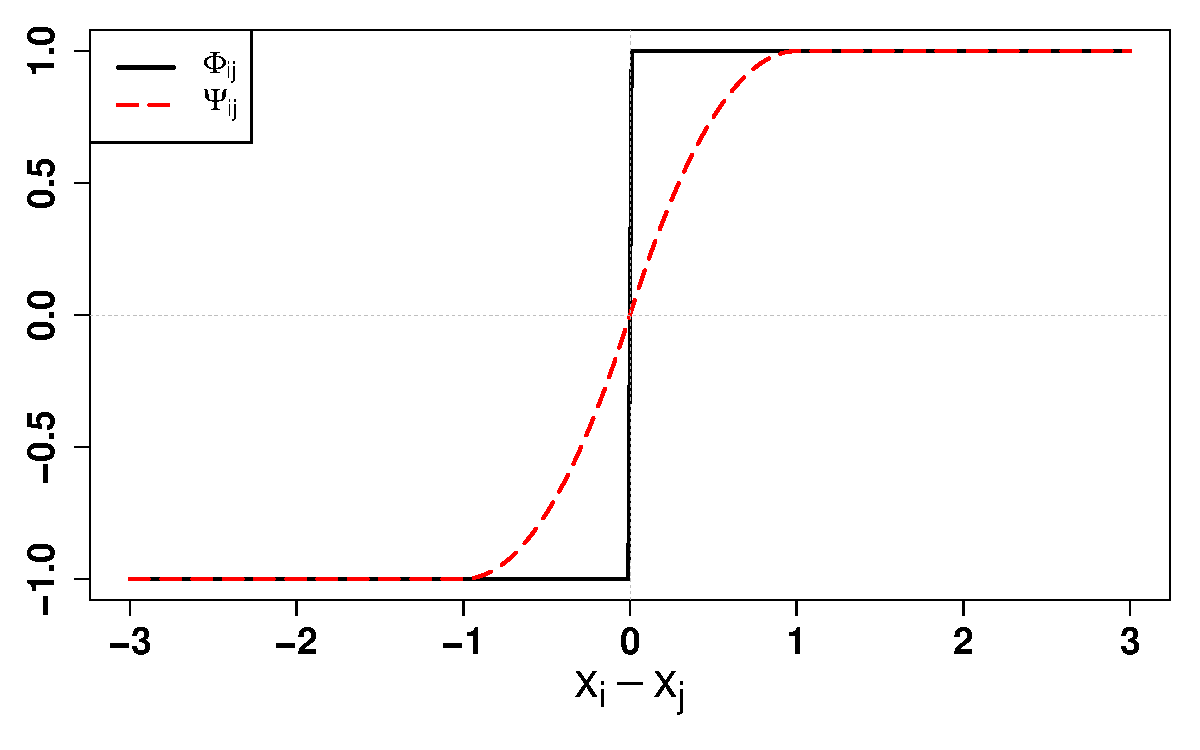
\includegraphics[width=0.6\textwidth]{ch-kendall/figures/smoothheaviside}
\caption{Smooth approximation (in red) of the Heaviside function (in black) used to define the mapping \eqref{eq2:smoothmap} for $a=1$.}
\label{fig2:smoothheaviside}
\end{center}
\end{figure} 


Although the smoothed kernel \eqref{eq2:G} can be an interesting alternative to the Kendall kernel \eqref{eq2:kdtALL}, we unfortunately lose for $G$ the computational trick that allows to compute $K_\tau$ in $O(n\log n)$. Specifically, we have two ways to compute $G$:

\noindent {\bf (i) Exact evaluation.} The first alternative is to compute explicitly the $n\choose 2$-vector representation $\Psi$ in the feature space, and then take the dot product to obtain $G$. While the kernel evaluation is exact, an analytic form of the smoothed mapping \eqref{eq2:Gkernel} is required and the computational cost is linear with the dimension of the feature space, i.e., $O(n^2)$.

\noindent {\bf (ii) Monte Carlo approximation.} The second alternative requires the observation that the smoothed mapping $\Psi(\xb) = \mathbb{E}\Phi(\tilde{\xb})$ appears in the form of expectation and can thus be  approximated by a $D$-sample mean of jittered points mapped by $\Phi$ into the feature space:
\begin{equation*}\label{eq2:mcpsi}
\Psi_D(\xb) = \frac{1}{D}\sum_{j=1}^D \Phi(\tilde{\xb}^j) \,,
\end{equation*}
where $\tilde{\xb}^1,\ldots,\tilde{\xb}^D$ are i.i.d. noisy versions of $\xb$. The dot product induces a kernel:
\begin{equation}\label{eq2:mc}
G_D(\xb,\xb') = \Psi_D(\xb)^\top \Psi_D(\xb') = \frac{1}{D^2} \sum_{i=1}^D \sum_{j=1}^D K_\tau\br{\tilde{\xb}^i , \tilde{\xb}'^j}\,,
\end{equation}
which is a $D^2$-sample empirical estimate of $G(\xb,\xb') = \mathbb{E} K_\tau(\tilde{\xb},\tilde{\xb}')$ when $\xb,\xb'$ are independently jittered with identically distributed noise. Since $K_\tau$ is of computational complexity $O(n\log n)$, computing $G_D$ requires $O(D^2 n \log n)$.


Note that the second alternative is faster to compute than the first one as long as, up to constants, $D^2 < n / \log n$, and small values of $D$ are thus favored on account of computational consideration. In that case, however, the approximation performance can be unappealing. To better understand the trade-off between the two alternatives, the question should be addressed upon how large $D$ should be so that the approximation error is not detrimental to the performance of a learning algorithm if we use the approximate kernel $G_D$ instead of $G$. Lemma \ref{lem2:concentration} provides a first answer to this question, showing that the approximation error of the kernel is upper bounded by $O(1/\sqrt{D})$ with high probability:
\begin{lemma}\label{lem2:concentration}
For any $0<\delta<1$, the following holds:

\noindent (a) For any $\xb\in\RR^n$, with probability greater than $1-\delta$,
$$
\nm{\Psi_D(\xb) - \Psi(\xb)} \leq \frac{1}{\sqrt{D}} \br{ 2+ \sqrt{8\log\frac{1}{\delta}}}\,.
$$

\noindent (b) For any $\xb_1, \ldots, \xb_m \in \RR^n$, with probability greater than $1-\delta$,
$$
\sup_{i=1,\ldots,m}\nm{\Psi_D(\xb_i) - \Psi(\xb_i)} \leq \frac{1}{\sqrt{D}} \br{ 2+ \sqrt{8\log\frac{m}{\delta}}}\,.
$$
\end{lemma}

\begin{proof}
For any $\xb\in\RR^n$, note that $\nm{\Phi(\xb)} \leq 1$. We can therefore apply \cite[Example 6.3]{Boucheron2013Concentration} to the random vector $X_j = \Phi(\tilde{\xb}^j) - \Psi(\xb)$ that satisfies $\EE X_j = 0$ and $\nm{X_j}\leq 2$ a.s. to get, for any $u\geq 2/\sqrt{D}$,
$$
\mathbb{P}\br{\nm{\Psi_D(\xb) - \Psi(\xb)} \geq u} \leq \exp \Bigg(-\frac{\br{u\sqrt{D}-2}^2}{8}\Bigg)\,.
$$
We recover (a) by setting the right-hand side equal to $\delta$ and solving for $u$. (b) then follows by a simple union bound.
\end{proof}

The uniform approximation bound of Lemma \ref{lem2:concentration} in turn implies that learning with the approximate kernel $G_D$ can be almost as good with the kernel $G$, as we now discuss. For that purpose, let us consider for example the case where the smoothed kernel $G$ is used to train a Support Vector Machine (SVM) from a training set $\mathcal{D}=\{(\mathbf{x}_i,y_i)\}_{i=1}^m\subset (\RR^n \times \{-1,+1\})^m$, specifically to estimate a function $h(\mathbf{x})=\mathbf{w}^\top \Psi(\mathbf{x})$ by solving
\begin{equation}
\label{eq2:svm}
\min_{\mathbf{w}} F(\mathbf{w})=\frac{\lambda}{2} \|\mathbf{w}\|^2 + \widehat{R}(\mathbf{w}),
\end{equation}
where $\widehat{R}(\mathbf{w})=\frac{1}{m}\sum_{i=1}^m \ell(y_i \mathbf{w}^\top \Psi(\mathbf{x}_i))$ is the empirical loss, with $\ell(y_i \mathbf{w}^\top \Psi(\mathbf{x}_i))=\max(0, 1-y_i \mathbf{w}^\top \Psi(\mathbf{x}_i))$ the hinge loss associated to the $i$-th point, $\lambda$ the regularization parameter. Now suppose that instead of training the SVM with smoothed feature mapping on the original points $\{\Psi(\xb_i)\}_{i=1,\dots,m}$, we first randomly jitter $\{\xb_i\}_{i=1,\dots,m}$ $D$ times at each point, resulting in $\{\tilde{\xb}_i^j\}_{i=1,\dots,m;j=1,\dots,D}$, and then replace each $\Psi(\xb_i)$ by the $D$-sample empirical average of jittered points mapped by $\Phi$ into the feature space, that is
$$
\Psi_D(\xb_i) := \frac{1}{D}\sum_{j=1}^D \Phi(\tilde{\xb}_i^j)\,.
$$
Note that $ \Psi_D(\xb_i)^\top \Psi_D(\xb_j)=G_D(\xb_i,\xb_j)$, hence training an SVM with the Monte Carlo approximate $G_D$ instead of exact version $G$ is equivalent to solving \eqref{eq2:svm} with $\{\Psi_D(\xb_i)\}_{i=1,\dots,m}$ in the hinge loss instead of $\{\Psi(\xb_i)\}_{i=1,\dots,m}$. Theorem \ref{thm2:approx} quantifies the approximation performance in terms of objective function $F$ which helps to answer the question on the trade-off between $G$ and $G_D$ in computational complexity and learning accuracy.


\begin{thm}\label{thm2:approx}
For any $0\leq\delta\leq 1$, the solution $\wh_D$ of the SVM trained with the Monte Carlo approximation \eqref{eq2:mc} with $D$ random-jittered samples for each training point satisfies, with probability greater than $1-\delta$,
$$
F(\wh_D) \leq \min_{\mathbf{w}} F(\mathbf{w}) +  \sqrt{\frac{8}{\lambda D}} \br{ 2+ \sqrt{8\log\frac{m}{\delta}}}\,.
$$
\end{thm}

\begin{proof}
Let $\wh$ be a solution to the original SVM optimization problem, and $\wh_D$ a solution to the perturbed SVM, i.e., a solution of
\begin{equation}
\label{eq2:svmD}
\min_{\mathbf{w}} F_D(\mathbf{w})=\frac{\lambda}{2} \|\mathbf{w}\|^2 + \widehat{R}_D(\mathbf{w}),
\end{equation}
with $\widehat{R}_D(\mathbf{w})=\frac{1}{m}\sum_{i=1}^m \ell(y_i \mathbf{w}^\top \Psi_D(\mathbf{x}_i))$. Since the hinge loss is $1$-Lipschitz, i.e., $|\ell(a)-\ell(b)|\leq |a-b|$ for any $a,b\in\RR$, we obtain that for any $\ub\in\RR^{n\choose 2}$: 
\begin{equation}\label{eq2:risklipschitz}
\begin{split}
\abs{\Rh(\ub)-\Rh_D(\ub)} &\leq \frac{1}{m}\sum_{i=1}^m \abs{\ub^\top\br{\Psi(\xb_i) - \Psi_D(\xb_i)}} \\
& \leq \nm{\ub} \sup_{i=1,\ldots,m}\nm{\Psi_D(\xb_i) - \Psi(\xb_i)}\,.
\end{split}
\end{equation}
Now, since $\wh_D$ is a solution of \eqref{eq2:svmD}, it satisfies
$$
\nm{\wh_D} \leq \sqrt{\frac{2F_D(\wh_D)}{\lambda}} \leq \sqrt{\frac{2F_D(0)}{\lambda}} = \sqrt{\frac{2}{\lambda}}\,,
$$
and similarly $\nm{\wh} \leq \sqrt{2/\lambda}$ because $\wh$ is a solution of the original SVM optimization problem. Using \eqref{eq2:risklipschitz} and these bounds on $\nm{\wh_D}$ and $\nm{\wh}$, we get
\begin{equation*}
\begin{split}
F(\wh_D) & - F(\wh) \\
& = F(\wh_D) - F_D(\wh_D) + F_D(\wh_D) - F(\wh)\\
&\leq F(\wh_D) - F_D(\wh_D) + F_D(\wh) - F(\wh)\\
&= \Rh(\wh_D)-\Rh_D(\wh_D) + \Rh_D(\wh) -\Rh(\wh)\\
& \leq \br{\nm{\wh_D} + \nm{\wh}} \sup_{i=1,\ldots,m}\nm{\Psi_D(\xb_i) - \Psi(\xb_i)}\\
& \leq \sqrt{\frac{8}{\lambda}} \sup_{i=1,\ldots,m}\nm{\Psi_D(\xb_i) - \Psi(\xb_i)} \,.
\end{split}
\end{equation*}
Theorem \ref{thm2:approx} then follows from Lemma \ref{lem2:concentration}.
\end{proof}


It is known that compared to the exact solution of \eqref{eq2:svm}, an $O(m^{-1/2})$-approximate solution is sufficient to reach the optimal statistical accuracy \cite{Bottou2008Tradeoffs}. This accuracy can be attained in our analysis when $D = O(m/\lambda)$, and since typically $\lambda \sim m^{-1/2}$ \cite{Steinwart2005Consistency}, this suggests that it is sufficient to take $D$ of order $m^{3/2}$. Going back to the comparison strategy of the two alternatives $G$ and $G_D$, we see that the computational cost of computing the full $m\times m$ Gram matrix with the exact evaluation is $O(m^2 n^2)$, while the cost of computing the approximate Gram matrix with $D=O(m^{3/2})$ random samples is $O(m^2 D^2 n \log n) = O(m^5 n \log n)$. This shows that, up to constants and logarithmic terms, the Monte Carlo approximation is interesting when $m = o(n^{1/3})$, otherwise the exact evaluation using explicit computation in the feature space is preferable.

Interestingly we can look at the extended Kendall kernel \eqref{eq2:G} to uncertain rankings from the perspective of Hilbert space embeddings of probability distributions \cite{Smola2007Hilbert}. In fact, for $x$ fixed, the smoothed mapping $\Psi(\xb) = \EE \Phi(\xb+\epsilon)$ is exactly an embedding for the distribution $\mathcal{P}$ of an additive noise $\epsilon$ in the reproducing kernel Hilbert space (RKHS) associated with Kendall kernel. As a consequence, the idea of smoothed kernel $G(\xb,\xb')$ for $\xb,\xb'\in \mathcal{X}$ is essentially equivalent to how \cite[Lemma 4]{Muandet2012Learning} defines kernels on two probability distributions from $\{\mathcal{P}+\xb | \xb \in \mathcal{X} \}$ using the Kendall kernel as the level-1 embedding kernel and linear inner product as the level-2 kernel in the feature space. As a result, given a fixed training set $\mathcal{D}$, training an SVM with $G$ in place of $K_\tau$ is equivalent to training a Flex-SVM instead of an ordinary SVM with $K_\tau$ \cite{Muandet2012Learning}. In this case, Theorem \ref{thm2:approx} provides an error bound in terms of the optimal accuracy for cases when training a Flex-SVM if exact evaluation of $G$ is intractable and its Monte Carlo approximate $G_D$ is employed. This serves to obtain a trade-off between computation complexity and approximation accuracy which is particularly interesting when we are working in high dimensions.








\section{Relation of the Mallows Kernel and the Diffusion Kernel on $\mathbb{S}_n$}
\label{sec2:group}

It is interesting to relate the Mallows kernel \eqref{eq2:mallows} to the diffusion kernel on the symmetric group proposed by \cite{Kondor2010Ranking}, which is the diffusion kernel \cite{Kondor2002Diffusion} on the Cayley graph of $\Sn$ generated by adjacent transpositions with left-multiplication. This graph, illustrated for a specific case of $n=4$ in Figure \ref{fig2:permutahedron}, is defined by $\mathcal{G}=(\mathcal{V},\mathcal{E})$ with $\mathcal{V}=\mathbb{S}_n$ as vertices, and undirected edge set $\mathcal{E}=\big\{ \{\sigma,\pi\sigma\} : \sigma\in \mathbb{S}_n,\pi\in Q \big\}$, where $Q=\{(i,i+1)|i=1,\dots,n-1\}$ the set of all adjacent transpositions. Note $Q$ is symmetric in the sense that $\pi\in Q \Leftrightarrow \pi^{-1}\in Q$, and the graph adjacency relation is a right-invariant relation, that is $\sigma \sim \sigma' \Leftrightarrow \sigma'\sigma^{-1}\in Q$. The corresponding graph Laplacian is the matrix $\Delta$ with
\begin{equation*}
	\Delta_{\sigma,\sigma'} = \left\{
		\begin{array}{ll}
			1 & \textrm{if } \sigma \sim \sigma' \\
			-(n-1) & \textrm{if } \sigma = \sigma' \\
			0 & \textrm{otherwise}
		\end{array}
	\right. ,
\end{equation*}
where $n-1$ is the degree of vertex $\sigma$ (number of edges connected with vertex $\sigma$), and the \emph{diffusion kernel} on $\Sn$ is finally defined as
\begin{equation}
	\label{eq2:diffusionkernel}
	K_{\textrm{dif}}^{\beta} (\sigma,\sigma') = [e^{\beta \Delta}]_{\sigma,\sigma'}
\end{equation}
for some diffusion parameter $\beta \in \mathbb{R}$, where $e^{\beta \Delta}$ is the matrix exponential. $K_{\textrm{dif}}^{\beta}$ is a right-invariant kernel on the symmetric group \cite[Proposition 2]{Kondor2010Ranking}, and we denote by $\kappa_{\textrm{dif}}^\beta$ the positive definite function induced by $K_{\textrm{dif}}^{\beta}$ such that $K_{\textrm{dif}}^{\beta}(\sigma,\sigma') = \kappa_{\textrm{dif}}^\beta (\sigma'\sigma^{-1}).$ Since the Mallows kernel $K_M^\lambda$ is straightforwardly right-invariant, we denote by $\kappa_M^\lambda$ the positive definite function induced by the Mallows kernel $K_M^\lambda$ such that $K_M^\lambda(\sigma,\sigma') = \kappa_M^\lambda (\sigma'\sigma^{-1}).$ One way to interpret the diffusion kernel \eqref{eq2:diffusionkernel} is by the heat equation on the Cayley graph
\begin{equation*}
	\frac{d}{d \beta} K_{\textrm{dif}}^{\beta} = \Delta K_{\textrm{dif}}^{\beta} \quad \mbox{ s.t. } K_{\textrm{dif}}^{\beta}|_{\beta=0}=I.
\end{equation*}
$K_{\textrm{dif}}^{\beta}$ is thus the product of a continuous process, expressed by the graph Laplacian $\Delta$, gradually transforming local structure $K_{\textrm{dif}}^{\beta}|_{\beta=0}=I$ to a kernel with stronger and stronger off-diagonal effects as $\beta$ increases.





\begin{figure}[!htbp]
\begin{center}
\centerline{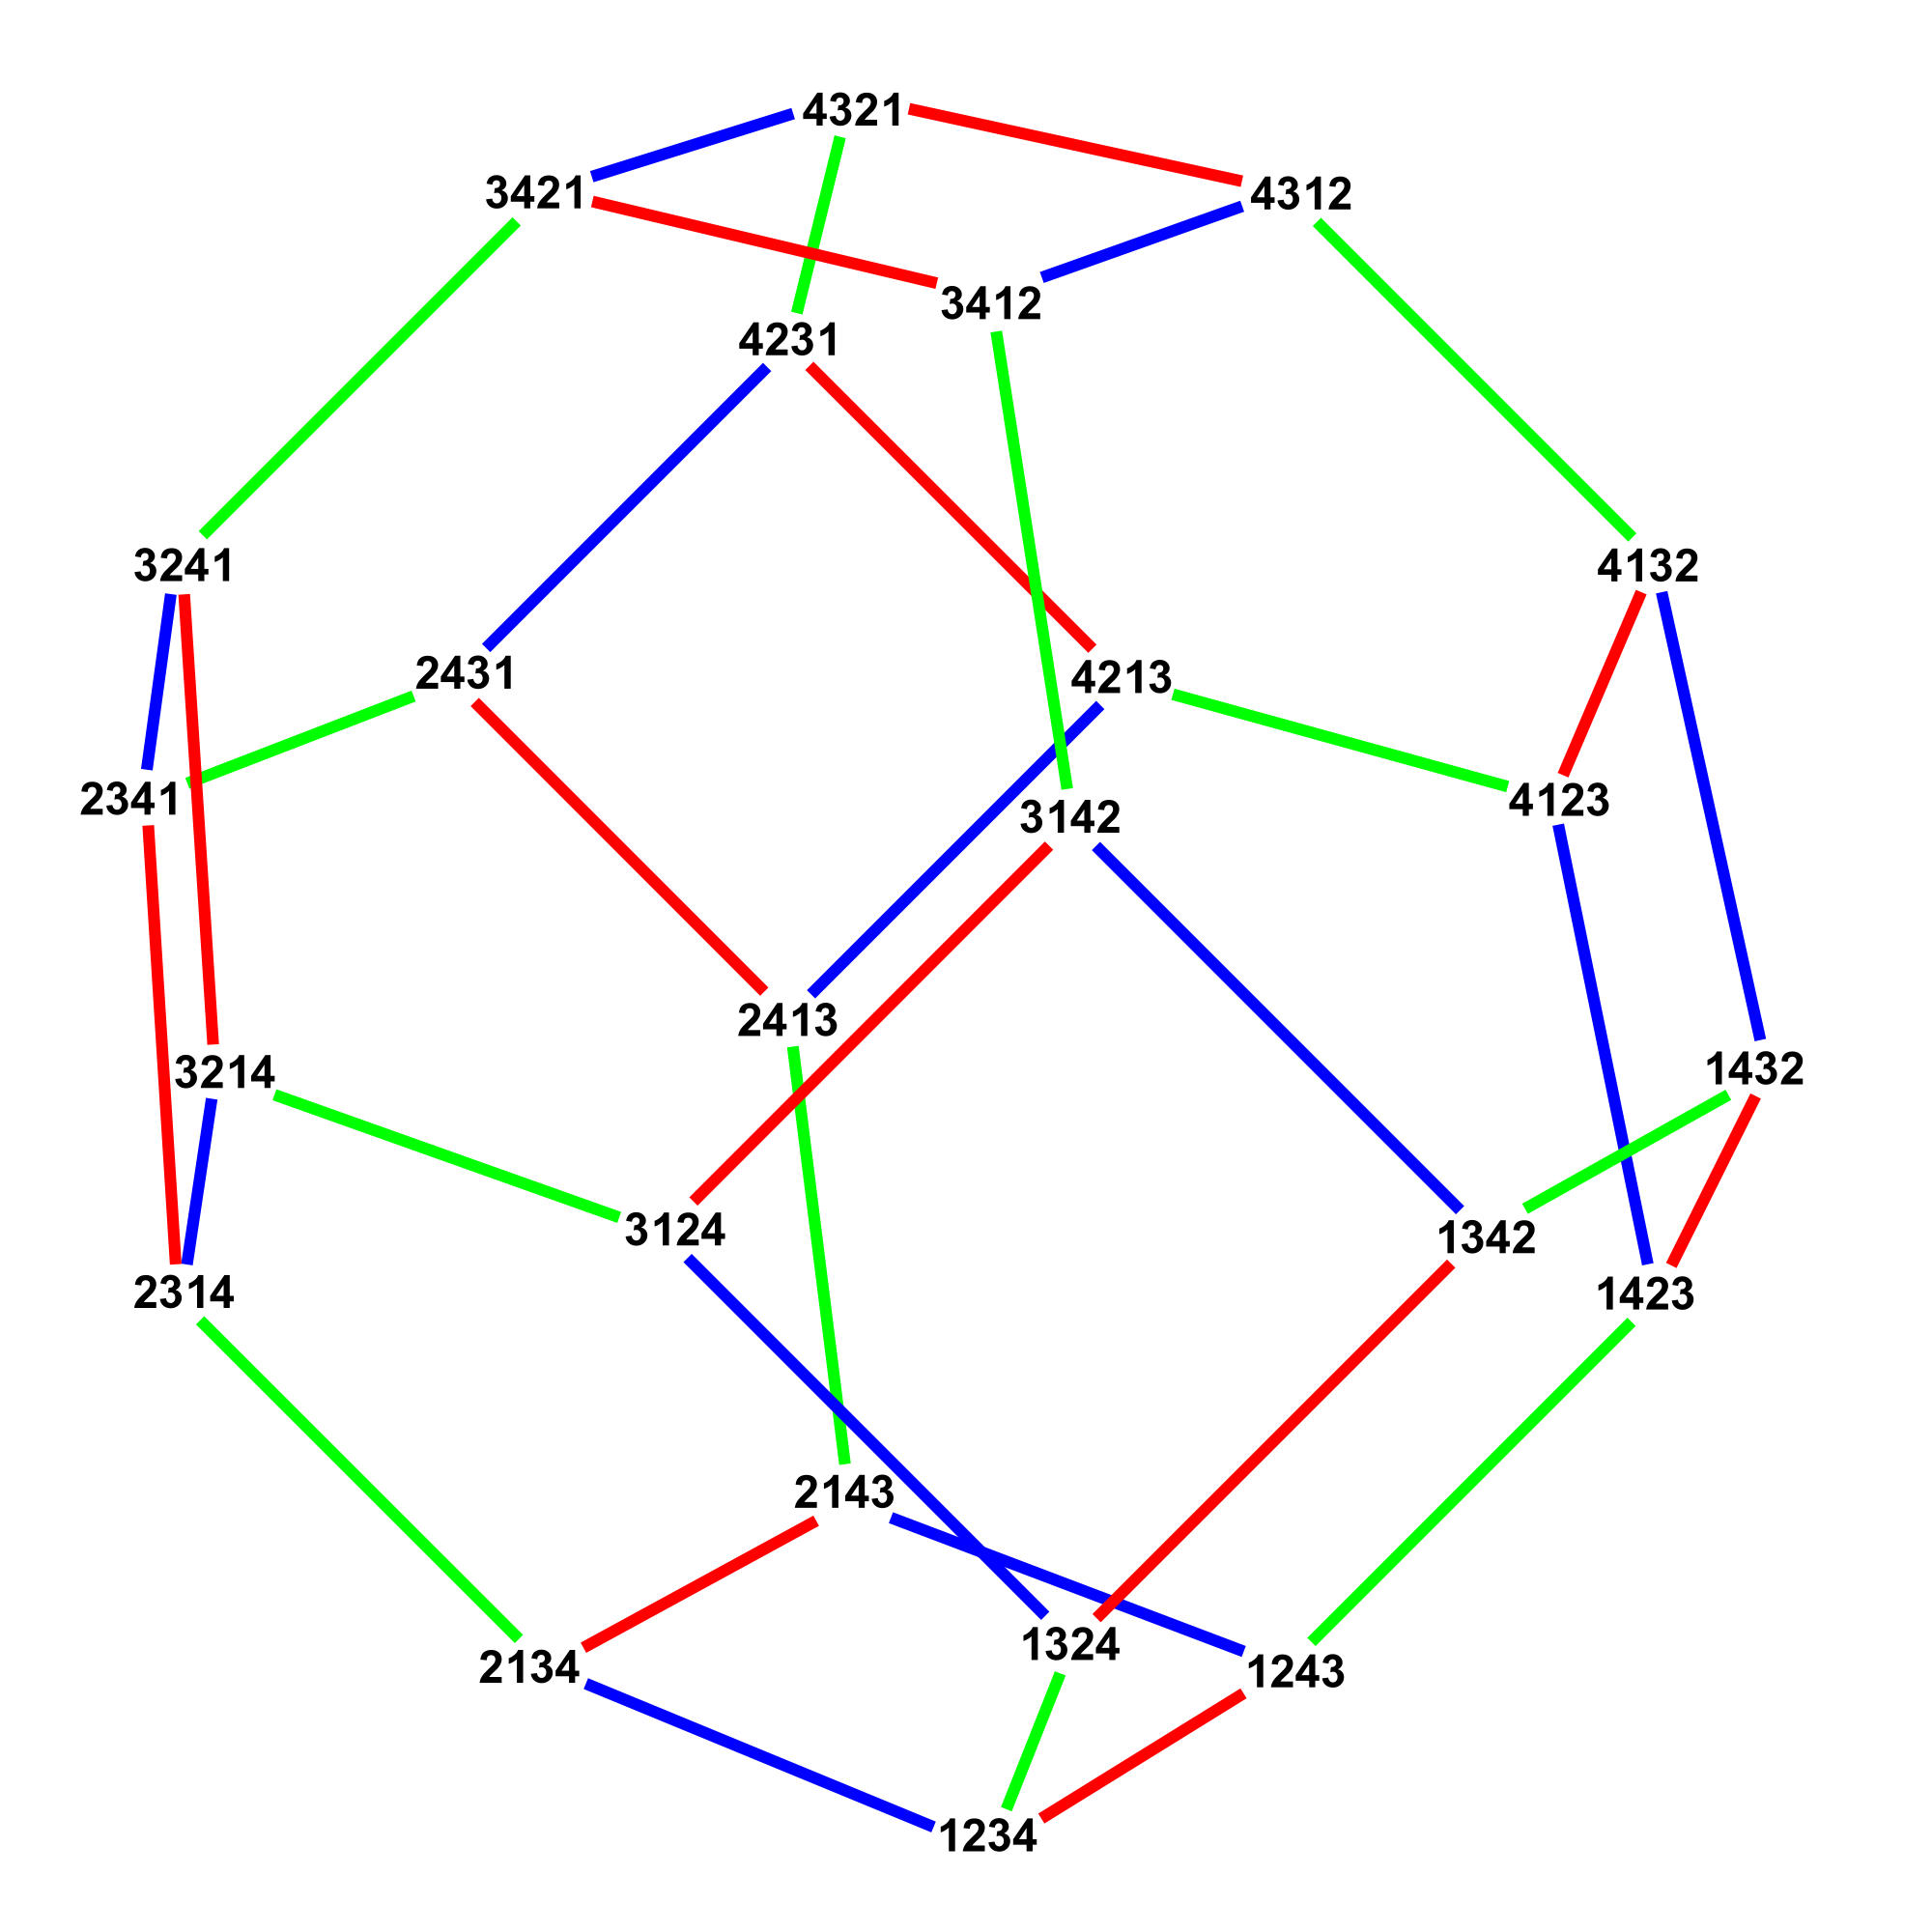
\includegraphics[width=0.6\textwidth]{ch-kendall/figures/permutahedron}}
\caption{Cayley graph of $\mathbb{S}_4$, generated by the transpositions (1 2) in blue, (2 3) in green, and (3 4) in red.}
\label{fig2:permutahedron}
\end{center}
\end{figure} 




Interestingly, the Mallows kernel can also be interpreted with the help of the Cayley graph. Indeed, it is well-known that the Kendall tau distance $n_d(\sigma,\sigma')$ is the minimum number of adjacent swaps required to bring $\sigma$ to $\sigma'$, i.e. $n_d(\sigma,\sigma')$ equals to the shortest path distance on the Cayley graph \cite[Exercise 7.73]{Drutu2017Geometric}, or simply written
\begin{equation*}
n_d(\sigma,\sigma')=d_{\mathcal{G}}(\sigma,\sigma') \,.
\end{equation*}
Different from the diffusion kernel for which communication between permutations is a diffusion process over the graph, the Mallows kernel 
$$K_{M}^{\lambda}(\sigma,\sigma')=e^{-\lambda n_d(\sigma,\sigma')}=e^{-\lambda d_{\mathcal{G}}(\sigma,\sigma')}$$ 
considers exclusively the shortest path over the graph when expressing the similarity between permutations $\sigma,\sigma'$. 






A notable advantage of the Mallows kernel over the diffusion kernel is that the Mallows kernel enjoys faster evaluation. On one hand if data instances are total rankings, i.e. $\sigma,\sigma'\in \mathbb{S}_n$, evaluating $K_{\textrm{dif}}^{\beta}(\sigma,\sigma')$ would require exponentiating an $n!$-dimensional Laplacian matrix by naive implementation, and can reduce to exponentiating matrices of smaller sizes by careful analysis in the Fourier space, which still remains problematic if working dimension $n$ is large \cite{Kondor2010Ranking}. However, evaluating $K_{M}^{\lambda}(\sigma,\sigma')$ only takes $O(n\log n)$ time. On the other hand if data instances are partial ranking of size $k\ll n$, i.e. $R,R'\subset \mathbb{S}_n$, and we take convolution kernel \eqref{eq2:partialranking} to extend the two kernels, the analysis of exploring the sparsity of the Fourier coefficients of the group algebra of partial rankings $R,R'$ of size $k$ reduces the evaluation of both the diffusion kernel and the Mallows kernel to $O((2k)^{2k+3})$ time, provided that the exponential kernel Fourier matrices $[\hat{\overline{\kappa}}(\mu)]_{\geq [\dots]_{n-k}}$ are precomputed before any kernel evaluations take place \cite[Theorem 13]{Kondor2010Ranking}.









\section{Application: Clustering and Modeling Rank Data}
\label{sec2:clustering}

In this section we illustrate the potential benefit of kernel-based algorithms using the Kendall and Mallows kernels for the purpose of unsupervised cluster analysis, i.e., partitioning a collection of rank data into sub-groups and/or estimating densities of a collection of rank data. This is in particular of great practical interest in social choice theory in order to explore the heterogeneity and identify typical sub-groups of voters with a common behavior to understand, for example, their political support for various parties \cite{Gormley2006Analysis,Gormley2008Exploring,Marden1996Analyzing}.


\subsection{Clustering with Kernel $k$-means}
\label{sec2:clusterkmeans}

Let $\cbr{\sigma_i}_{i=1}^m \subset \Sn$ be a collection of $m$ permutations representing, say, the preferences of customers over $n$ products or the votes of electorate over $n$ candidates. We aim at partitioning these permutations into $c \leq m$ clusters $\cbr{S_j}_{j=1}^c$. One approach to cluster rank data is to follow a method similar to $k$-means in the symmetric group. Assuming that each cluster $S_j$ has a ``center'' $\pi_j \in\Sn$ serving as a prototype permutation of that cluster, the classic $k$-means clustering attempts to put each point in the cluster with the nearest center so as to minimize the sum of Kendall tau distance of each permutation to the corresponding center of its cluster. Specifically, when the number of clusters $c$ is fixed, the objective is to find:
\begin{equation}\label{eq2:kmeans}
\underset{\cbr{S_j,\pi_j\in\Sn}}{\arg\min} \sum_{j=1}^c \sum_{i:\sigma_i\in S_j} n_d(\sigma_i,\pi_j) \,.
\end{equation}
Note that \eqref{eq2:kmeans} reduces to a single-ranking aggregation problem when $c=1$, where the center $\pi$ is commonly known as Kemeny consensus \cite{Kemeny1962Mathematical} which is NP-hard to find \cite{BartholdiIII1989Voting}. With the objective in \eqref{eq2:kmeans} being non convex, Lloyd's algorithm is usually employed to find local minima in an iterative manner consisting of two steps: the \emph{assignment step} assigns each point to its closest cluster, and the \emph{update step} updates each of the $c$ cluster centers using the points assigned to that cluster; the algorithm repeats until all the cluster centers remain unchanged in an iteration. While the assignment step is usually fast, the update step is indeed equivalent to solving a Kemeny consensus problem for each cluster, i.e., $\arg\min_{\pi_j\in\Sn} \sum_{i:\sigma_i\in S_j} n_d(\sigma_i,\pi_j)$. Since the exact Kemeny-optimal ranking is difficult to find, approximate techniques are usually employed in practice such as Borda Count \cite{Borda1781Memoire} or Copeland's method \cite{Copeland1951reasonable}.

As the Kendall tau distance is conditionally positive definite, we can propose as an alternative to use the kernel $k$-means approach \cite{Girolami2002Mercer,Zhang2002large} that relaxes the assumption that the cluster center are permutations, and instead works implicitly in the feature space where cluster centers can be any vector in $\RR^{{n\choose 2}}$ by considering the problem:
\begin{equation*}\label{eq2:kernelkmeans}
\underset{\big\{S_j,\mu_j\in\RR^{{n\choose 2}}\big\}}{\arg\min} \sum_{j=1}^c \sum_{i:\sigma_i\in S_j} \nm{\Phi(\sigma_i) - \mu_j}^2 \,,
\end{equation*}
for which local minima can be found efficiently by Algorithm \ref{alg:kernelkmeans}. Note that $\mu_j$ does not match a true permutation $\pi_j\in\Sn$ in general, and the Kemeny consensus problem in the update step is thus bypassed. It is worthwhile to note that the algorithm is not exclusive for clustering permutations, kernel $k$-means clustering can be applied respectively to total/partial/multivariate/uncertain rankings with appropriate kernels defined.

\begin{algorithm}[!htbp]
\caption{Kernel $k$-means for clustering heterogeneous rank data.}
{\bfseries Input:} a collection of permutations $\cbr{\sigma_i}_{i=1}^m$ and a kernel function $K$ over $\Sn$, or a kernel matrix evaluated between pairwise data points $\mathbf{K} = (K(\sigma_i,\sigma_j))_{1 \leq i,j \leq m}$; the number of clusters $c\leq m$.
\begin{algorithmic}[1]
 \STATE Randomly initialize cluster assignment for each data points and form $c$ clusters $S_1,\dots,S_c$.
 \STATE For each data point, find its new cluster assignment, i.e., for $i=1,\dots,m,$ 
 	$$j^*(\sigma_i) = \arg\min_j d_{ij} \,,$$
 	where
 	\begin{multline*}
 	d_{ij} := \nm{\Phi(\sigma_i) - \frac{1}{|S_j|} \sum_{\sigma_\ell\in S_j} \Phi(\sigma_\ell)}^2 \\
 	= K(\sigma_i,\sigma_i) - \frac{2}{|S_j|} \sum_{\sigma_\ell\in S_j} K(\sigma_i,\sigma_\ell)
 	+ \frac{1}{|S_j|^2} \sum_{\sigma_v,\sigma_\ell\in S_j} K(\sigma_v,\sigma_\ell) \,.
 	\end{multline*}
 \STATE Form updated clusters, i.e., for $j=1,\dots,c,$ 
 	$$S_j=\cbr{\sigma_i : j = j^*(\sigma_i), i=1,\dots,m} \,.$$
 \STATE Repeat 2-3 until all cluster assignments remain unchanged in an iteration.
\end{algorithmic}
{\bfseries Output:} Cluster assignments $\cbr{S_j}_{j=1}^c.$
\label{alg:kernelkmeans}
\end{algorithm}



\subsection{Mallows Mixture Model with Kernel Trick}
\label{sec2:clustermallows}

An alternative to $k$-means clustering is to consider mixture models, which provide a method for modeling heterogeneous population in data by assuming a mixture of standard models for rankings in each homogeneous sub-population. Mixture models not only allow to cluster data, but more generally to estimate a distribution on the space of permutation that can then be used for other purposes, such as combining evidences. One popular choice of probabilistic distribution over $\Sn$ is the Mallows model \cite{Mallows1957Non}, which takes the form in expressing the occurring probability of $\sigma$ by 
\begin{equation}\label{eq2:mallowspdf}
f(\sigma|\pi,\lambda) = C(\lambda) \exp[-\lambda n_d(\sigma,\pi)] \,,
\end{equation}
where the central ranking $\pi\in\Sn$ and the precision $\lambda\geq 0$ are model parameters, and the normalization constant $C(\lambda) = 1 / \sum_{\sigma'\in\Sn} \exp[-\lambda n_d(\sigma',\pi)]$ is chosen so that $f(\cdot|\pi,\lambda)$ is a valid probability mass function over $\Sn$. Notably, $C(\lambda)$ does not depend on the center $\pi$ due to the symmetry of $\Sn$. 


We follow the mixture modeling setup in \cite{Murphy2003Mixtures}. Now suppose that a population consists of $c$ sub-populations, a Mallows mixture model assumes that an observation comes from group $j$ with probability $p_j\geq 0$ for $j=1,\dots,c$ and, given that the observation belongs to sub-population $j$, it is generated from a Mallows model with central ranking $\pi_j$ and precision $\lambda_j$, i.e., the occurring probability of $\sigma$ in the Mallows mixture model is written as
\begin{equation}\label{eq2:mallowsf}
f(\sigma) = \sum_{j=1}^c p_j f(\sigma|\pi_j,\lambda_j) = \sum_{j=1}^c p_j C(\lambda_j) \exp[-\lambda_j n_d(\sigma,\pi_j)] \,.
\end{equation}
Denoting $\underline{\pi} = \cbr{\pi_j}_{j=1}^c$, $\underline{\lambda}=\cbr{\lambda_j}_{j=1}^c$, $\underline{p}=\cbr{p_j}_{j=1}^c$ such that $\sum_{j=1}^c p_j=1$, the log-likelihood of a collection of $m$ i.i.d. permutations $\underline{\sigma}=\cbr{\sigma_i}_{i=1}^m$ is therefore:
\begin{equation}\label{eq2:mallowsL}
L(\underline{\pi},\underline{\lambda},\underline{p}|\underline{\sigma}) = \sum_{i=1}^m \log f(\sigma_i)
= \sum_{i=1}^m \log \cbr{\sum_{j=1}^c p_j C(\lambda_j) \exp[-\lambda_j n_d(\sigma_i,\pi_j)]} \,.
\end{equation}
The Mallows mixture model is usually fitted by maximum likelihood using the EM algorithm. Specifically, by introducing latent (membership) variables $\underline{z} = \cbr{z_{ij}:i=1,\dots,m,j=1,\dots,c}$ where $z_{ij} = 1$ if $\sigma_i$ belongs to group $j$ and $0$ otherwise, the complete log-likelihood of data is
\begin{equation*}
L_C(\underline{\pi},\underline{\lambda},\underline{p}|\underline{\sigma},\underline{z}) = \sum_{i=1}^m \sum_{j=1}^c z_{ij}[\log p_j + \log C(\lambda_j) - \lambda_j n_d(\sigma_i,\pi_j)] \,.
\end{equation*}
The EM algorithm can be implemented to find local maximum likelihood estimates following two steps iteratively until convergence: the \emph{E-step} calculates the expected value of membership variables $\underline{\hat{z}}$ conditioned on the current estimates of the model parameters $\underline{\pi},\underline{\lambda},\underline{p}$, and the \emph{M-step} updates the model parameters $\underline{\pi},\underline{\lambda},\underline{p}$ by maximizing the expected complete log-likelihood $\hat{L}_C = L_C(\underline{\pi},\underline{\lambda},\underline{p}|\underline{\sigma},\underline{\hat{z}})$ where membership variables are replaced by their expected values. The final estimate $\hat{z}_{ij}$ amounts to our belief of $\sigma_i$ belonging to group $j$, and can thus be used to form clusters $\cbr{S_j}_{j=1}^c$ serving a partition of data where
\begin{equation}\label{eq2:mallowscluster}
S_j=\cbr{\sigma_i : \hat{z}_{ij} = \max_{\ell} \hat{z}_{i\ell}, i=1,\dots,m} \,.
\end{equation}


A closer look at the EM algorithm reveals that optimizing $\hat{L}_C$ with respect to $\underline{\pi}$ alone in the M-step is indeed equivalent to finding a (weighted) Kemeny consensus for each group, i.e., solving $\arg\min_{\pi_j\in\Sn} \sum_{i=1}^m \hat{z}_{ij} n_d(\sigma_i,\pi_j),$ for which exact solution is difficult as above-mentioned in the context of $k$-means clustering. Similarly to the idea of kernel $k$-means in contrast to classic $k$-means, we propose to seek ways to bypass the Kemeny consensus problem by working in the feature space instead. Note that the Mallows probability mass function \eqref{eq2:mallowspdf} is equivalently written as $f(\sigma|\pi,\lambda) \propto \exp \sqb{-\lambda \nm{\Phi(\sigma)-\Phi(\pi)}^2}$ up to a constant scaling on $\lambda$ by using \eqref{eq2:distance}, we propose to relax the constraint that the center has to match a true permutation $\pi\in\Sn$ and consider the following two alternatives in place of $f$ following the mixture modeling approach stated above:

\noindent {\bf (i) Kernel Mallows.} The Mallows probability mass function over $\Sn$ \eqref{eq2:mallowspdf} is generalized to admit any point in the feature space $\mu\in\RR^{{n\choose 2}}$ to be the population center, i.e.,
\begin{equation}\label{eq2:kernelmallows}
g(\sigma|\mu,\lambda) = C(\mu,\lambda) \exp \sqb{-\lambda \nm{\Phi(\sigma)-\mu}^2} \,,
\end{equation}
where the normalization constant $C(\mu,\lambda) = 1 / \sum_{\sigma'\in\Sn} \exp \sqb{-\lambda \nm{\Phi(\sigma')-\mu}^2}$ is chosen so that $g(\cdot|\mu,\lambda)$ is a valid probability mass function over $\Sn$. Notably, $C(\mu,\lambda)$ now depends on the center $\mu$ as well.

If we replace the probability mass function of classic Mallows $f$ in \eqref{eq2:mallowsL} by that of kernel Mallows $g$, the Kemeny consensus problem is averted when the EM algorithm is used to fit a local maximum likelihood estimate. However, another computational setback arises that the expected complete log-likelihood $\hat{L}_C$ to maximize in the M-step of the EM algorithm is separately concave with respect to $\mu$ or $\lambda$, but not jointly concave. Hence alternating optimization is often used in practice with the caveats of intensive computation and no guarantee to attain global optima for the M-step optimization at each iteration.


\noindent {\bf (ii) Kernel Gaussian.} Note that \eqref{eq2:kernelmallows} has a similar form to the Gaussian density, therefore we consider for $\sigma\in\Sn$,
\begin{equation}\label{eq2:kernelgaussian}
g^{\dagger} (\sigma|\mu,\lambda) = \sqrt{\br{\frac{\lambda}{\pi}}^{{n\choose 2}}} \exp \sqb{-\lambda \nm{\Phi(\sigma)-\mu}^2} \,,
\end{equation}
which is exactly $\mathcal{N}(\Phi(\sigma) | \mu, (2\lambda)^{-1} I )$, i.e., the ${n\choose 2}$-dimensional Gaussian distribution with mean $\mu$ and isotropic covariance matrix $(2\lambda)^{-1} I$ injected by $\Phi(\sigma)$. Notably, $g^{\dagger} (\cdot|\mu,\lambda)$ is not a valid probability mass function over $\Sn$.

The mixture modeling approach stated above using $g^{\dagger}$ instead of $f$ is in fact equivalently stated in Algorithm \ref{alg:kernelgaussian}. It is worthwhile to note that the algorithm also applies to total/partial/multivariate/uncertain rankings with appropriate kernels defined as \cite[Table 2]{Wang2003Kernel} provides the counterpart of Algorithm \ref{alg:kernelgaussian} in case that a kernel matrix evaluated between data points is given instead. However, since $g^{\dagger}$ itself is not a valid probability mass function over $\Sn$, an evident drawback is that we now lose the probabilistic interpretation of the mixture distribution as in \eqref{eq2:mallowsf}.


\begin{algorithm}[!htbp]
\caption{Kernel trick embedded Gaussian mixture model for clustering heterogeneous rank data.}
{\bfseries Input:} a collection of permutations $\cbr{\sigma_i}_{i=1}^m$ and a kernel function $K$ over $\Sn$; the number of clusters $c\leq m$.
\begin{algorithmic}[1]
 \STATE Compute feature points $\Phi(\sigma_i) \in \RR^{{n \choose 2}}$ mapped by the Kendall embedding.
 
 \STATE Fit a Gaussian mixture model for $\cbr{\Phi(\sigma_i)}_{i=1}^m$ in $\RR^{{n \choose 2}}$ using maximum likelihood with the EM algorithm under the constraint of isotropic covariance matrix, i.e., $\Sigma=(2\lambda)^{-1}I$.
 
 \STATE Use the membership estimates $\underline{\hat{z}}$ to form clusters by \eqref{eq2:mallowscluster}.
\end{algorithmic}
{\bfseries Output:} Cluster assignments $\cbr{S_j}_{j=1}^c.$
\label{alg:kernelgaussian}
\end{algorithm}



\subsection{Experiments}
\label{sec2:clusterexp}


\noindent {\bf Clustering 1980 APA election data.} In the 1980 American Psychological Association (APA) presidential election, voters were asked to rank $5$ candidates in order of preference, and $5738$ votes in form of total rankings were reported and thus used in our experiment. The dataset was thoroughly studied by \cite{Diaconis1988Group}.



We first use $k$-means approaches to cluster the data. We compare the proposed kernel $k$-means algorithm (Algorithm \ref{alg:kernelkmeans} with Kendall kernel $K_{\tau}$) to the classic $k$-means algorithm formulated as \eqref{eq2:kmeans}. For the classic $k$-means where cluster centers are required to be a prototype permutation, three methods are employed in the center-update step for each iteration: brute-force search of Kemeny-optimal ranking, approximate ranking induced by Borda Count and Copeland's method. In each case, we vary the number of clusters ranging from $2$ to $10$ and the algorithm is repeated $50$ times with randomly initialized configurations for each fixed number of clusters. We observe from Figure \ref{fig2:kmeans-time} that the kernel $k$-means or classic $k$-means with approximate centers runs much faster than optimal $k$-means for which the Kemeny-optimal ranking is time-consuming to find by a brute-force search. Further, Figure \ref{fig2:kmeans-silhouette} shows that the kernel $k$-means outperforms all three methods based on classic $k$-means in terms of the average silhouette scores of the clustering results, which justifies that the kernel $k$-means splits the data into more consistent sub-groups in the sense that instances, measured by Kendall tau distance on average, are more similar in the same cluster and more dissimilar in different clusters.



\begin{figure}[!htbp]
\centering
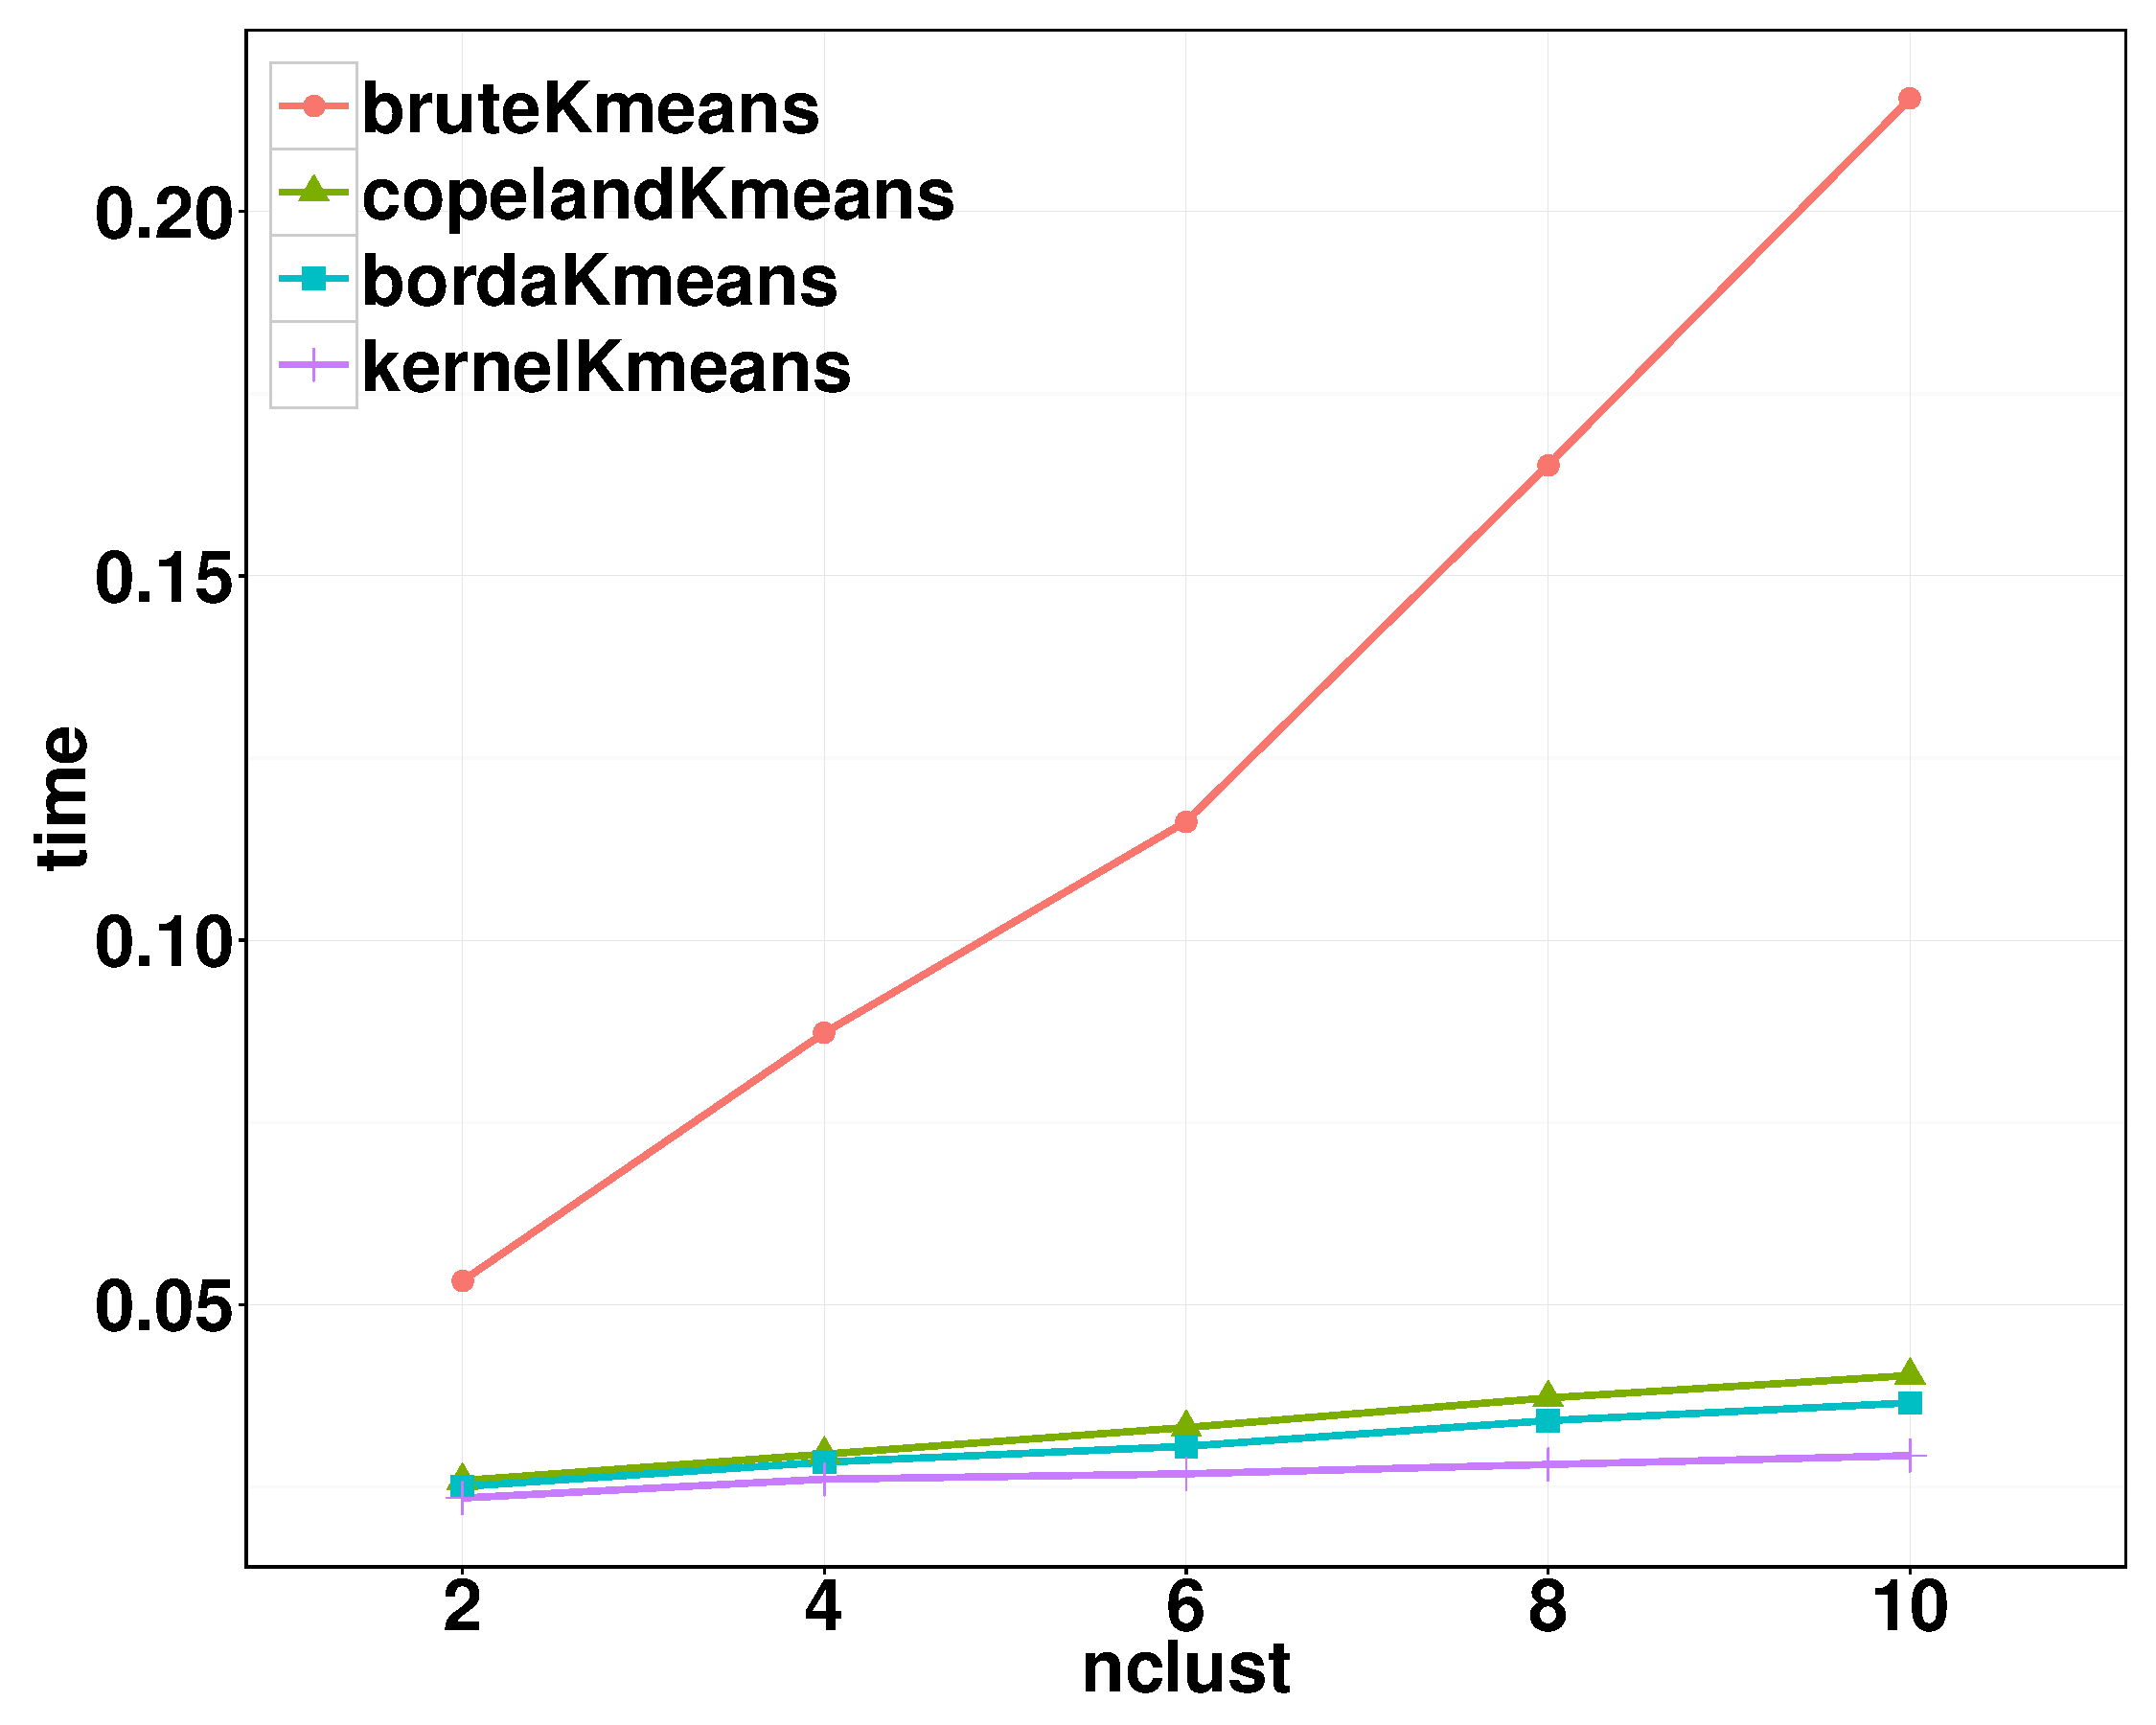
\includegraphics[width=0.6\textwidth]{ch-kendall/cluster_results/kmeans-time}\caption{Computational time (in seconds) of $k$-means algorithms per run across different number of clusters.}
\label{fig2:kmeans-time}
\end{figure}

\begin{figure}[!htbp]
\centering
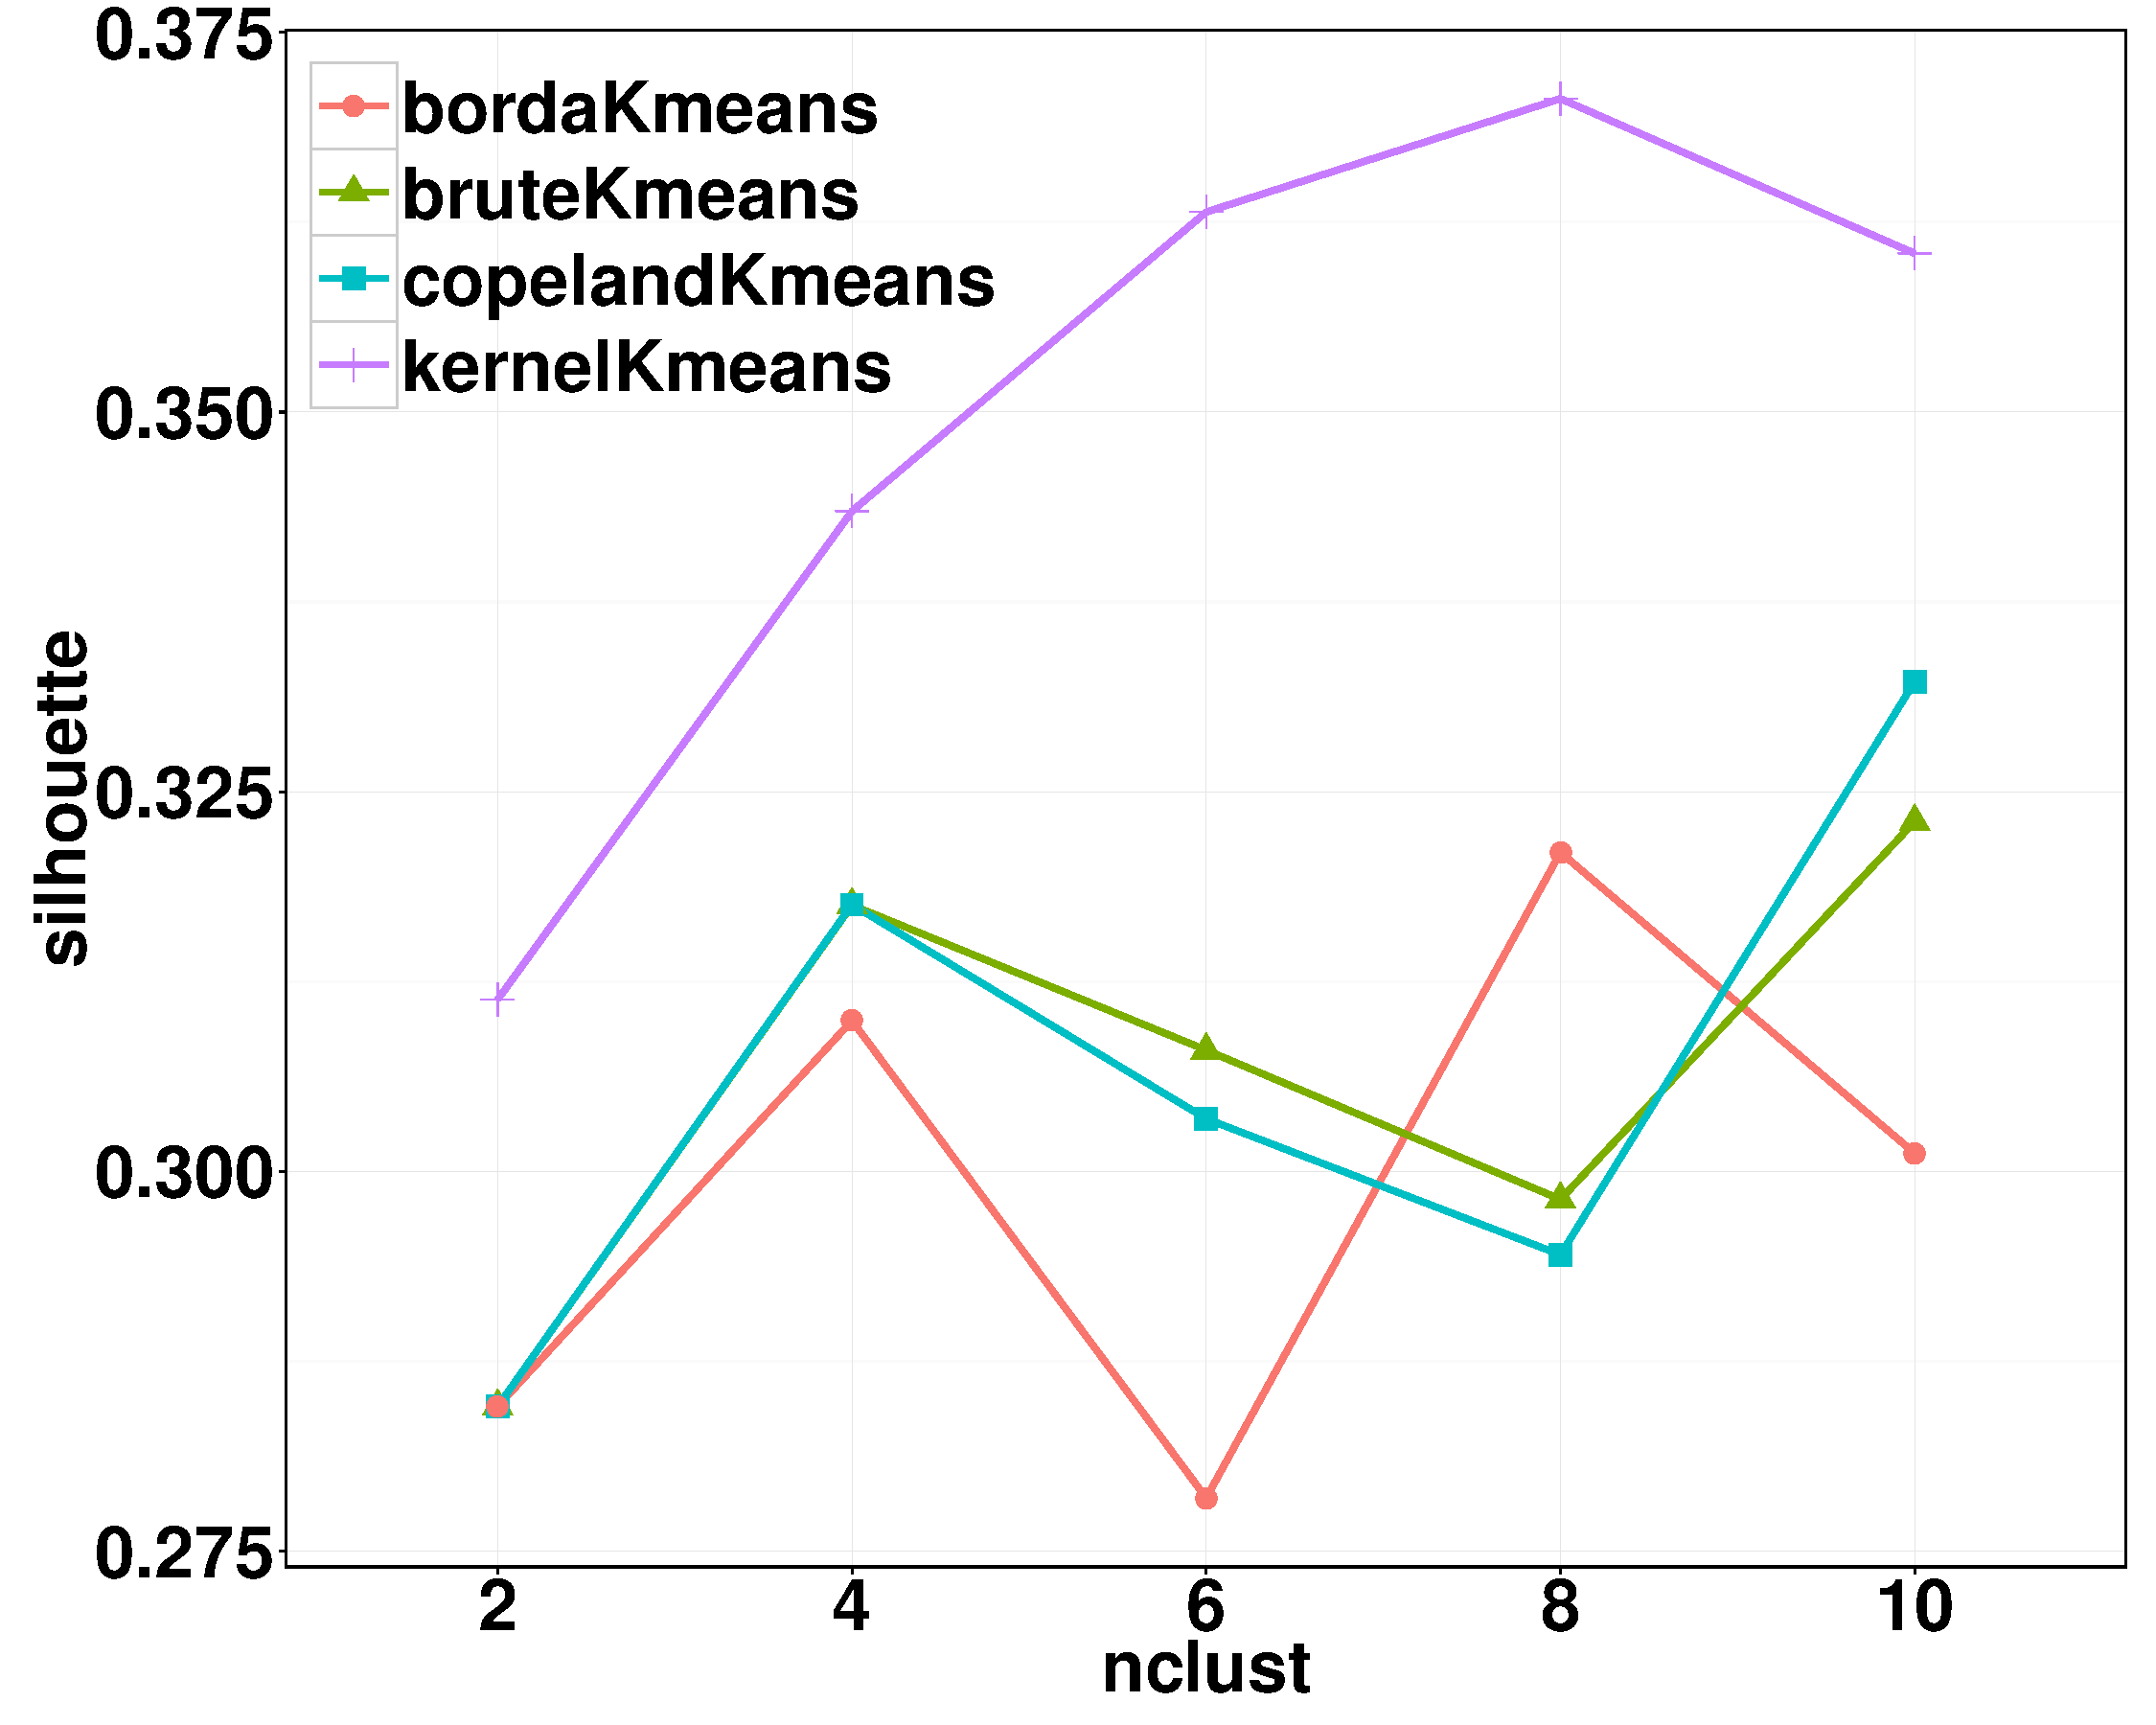
\includegraphics[width=0.6\textwidth]{ch-kendall/cluster_results/kmeans-silhouette}
\caption{Average silhouette scores of $k$-means methods across different number of clusters.}
\label{fig2:kmeans-silhouette}
\end{figure}



Further, good clustering algorithms are supposed be robust to ``perturbation'' in data, in the sense that clusters formed by running an algorithm on bootstrap replicas of the original data should be similar. In other words, if we bootstrap the complete dataset twice and form a clustering with respect to each, the two clustering assignments should be close to each other. Note that in order to measure the similarity of two clustering assignments, we use the (adjusted) Rand index defined by the percentage of instance pairs falling in the same or in different clusters by the two assignments \cite{Hubert1985Comparing}. We now compare the stability performance of the proposed kernel $k$-means and other $k$-means algorithms. Specifically, for each fixed number of clusters, we repeatedly use a bootstrap replica of the dataset to search for centroids returned by running $k$-means algorithms, and partition the original dataset with these identified centroids. The Rand index for two such clustering assignments is computed and the computation is repeated for 100 times accounting for the random process of bootstrapping. Results are shown in Figure \ref{fig2:kmeans-stability}. We observe that, for each fixed number of clusters, kernel $k$-means has higher stability scores than the classic $k$-means algorithms in general. Notably, the discrepancy between kernel $k$-means and the others in terms of their stability performance is even sharper when the number of clusters becomes large. In conclusion, evidence advocates again the use of kernel $k$-means over classic $k$-means algorithms in clustering rank data.


\begin{figure}[!htbp]
\begin{center}
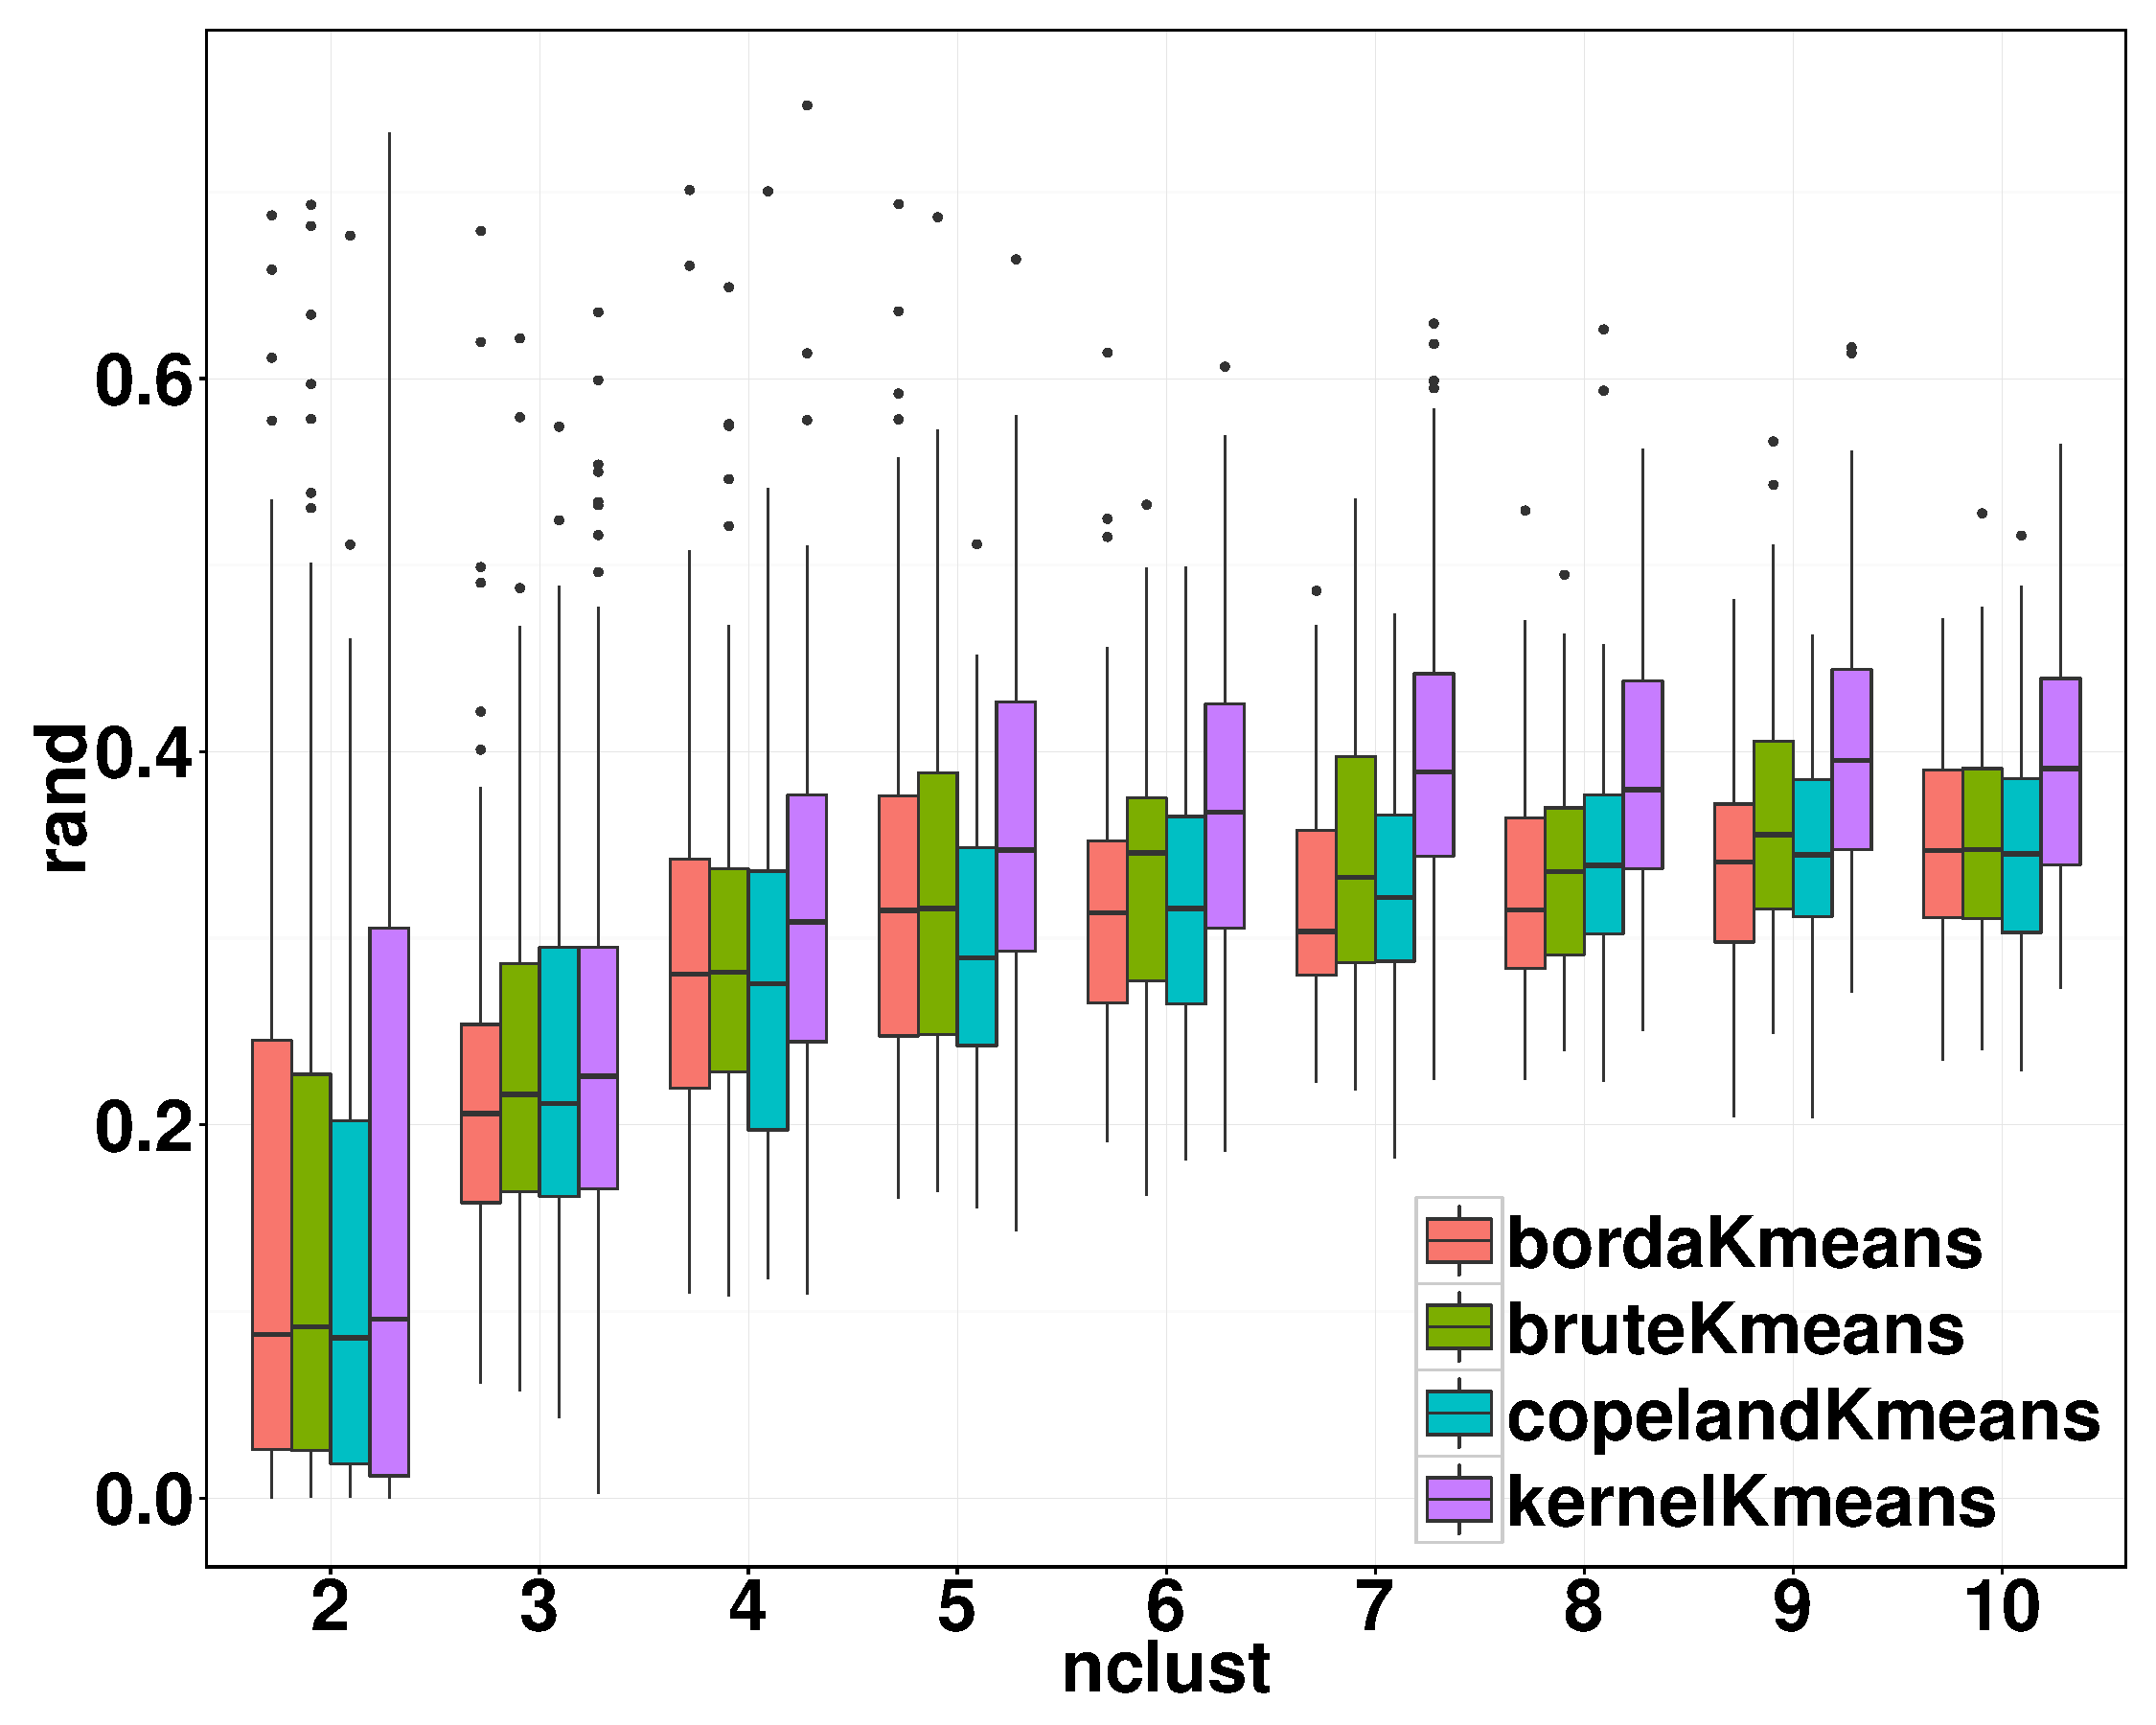
\includegraphics[width=0.6\textwidth]{ch-kendall/cluster_results/kmeans-stability}
\caption{Across different number of clusters, Rand index between clustering assignments by running $k$-means algorithm on bootstrap replicas of the 1980 APA election data. For each fixed number of clusters, the boxplot represents the variance over 100 repeated runs.}
\label{fig2:kmeans-stability}
\end{center}
\end{figure} 


Mixture modeling is then used to fit the data and a partition of the votes is converted from the fitted models forming a clustering result. Baseline models are the Mallows mixture models fitted by the EM algorithm \cite{Murphy2003Mixtures} using three different center-update algorithms at each iteration: brute-force search for Kemeny-optimal ranking, approximate ranking induced by Borda Count and Copeland's method. As proposed in this chapter, we embed the kernel trick in Mallows mixture modeling with two alternatives $g$ \eqref{eq2:kernelmallows} and $g^{\dagger}$ \eqref{eq2:kernelgaussian} in place of $f$ \eqref{eq2:mallowspdf}. In each case, we vary the number of clusters ranging from $2$ to $10$ and the algorithm is repeated $50$ times with randomly initialized configurations for each fixed number of clusters. As shown in Figure \ref{fig2:mallows-silhouette}, modeling a Gaussian mixture to data in the feature space, or equivalently using $g^{\dagger}$ instead of $f$, provides a preferable split of the data into sub-groups with higher average silhouette scores across different number of clusters selected \emph{a priori}.


\begin{figure}[!htbp]
\centering
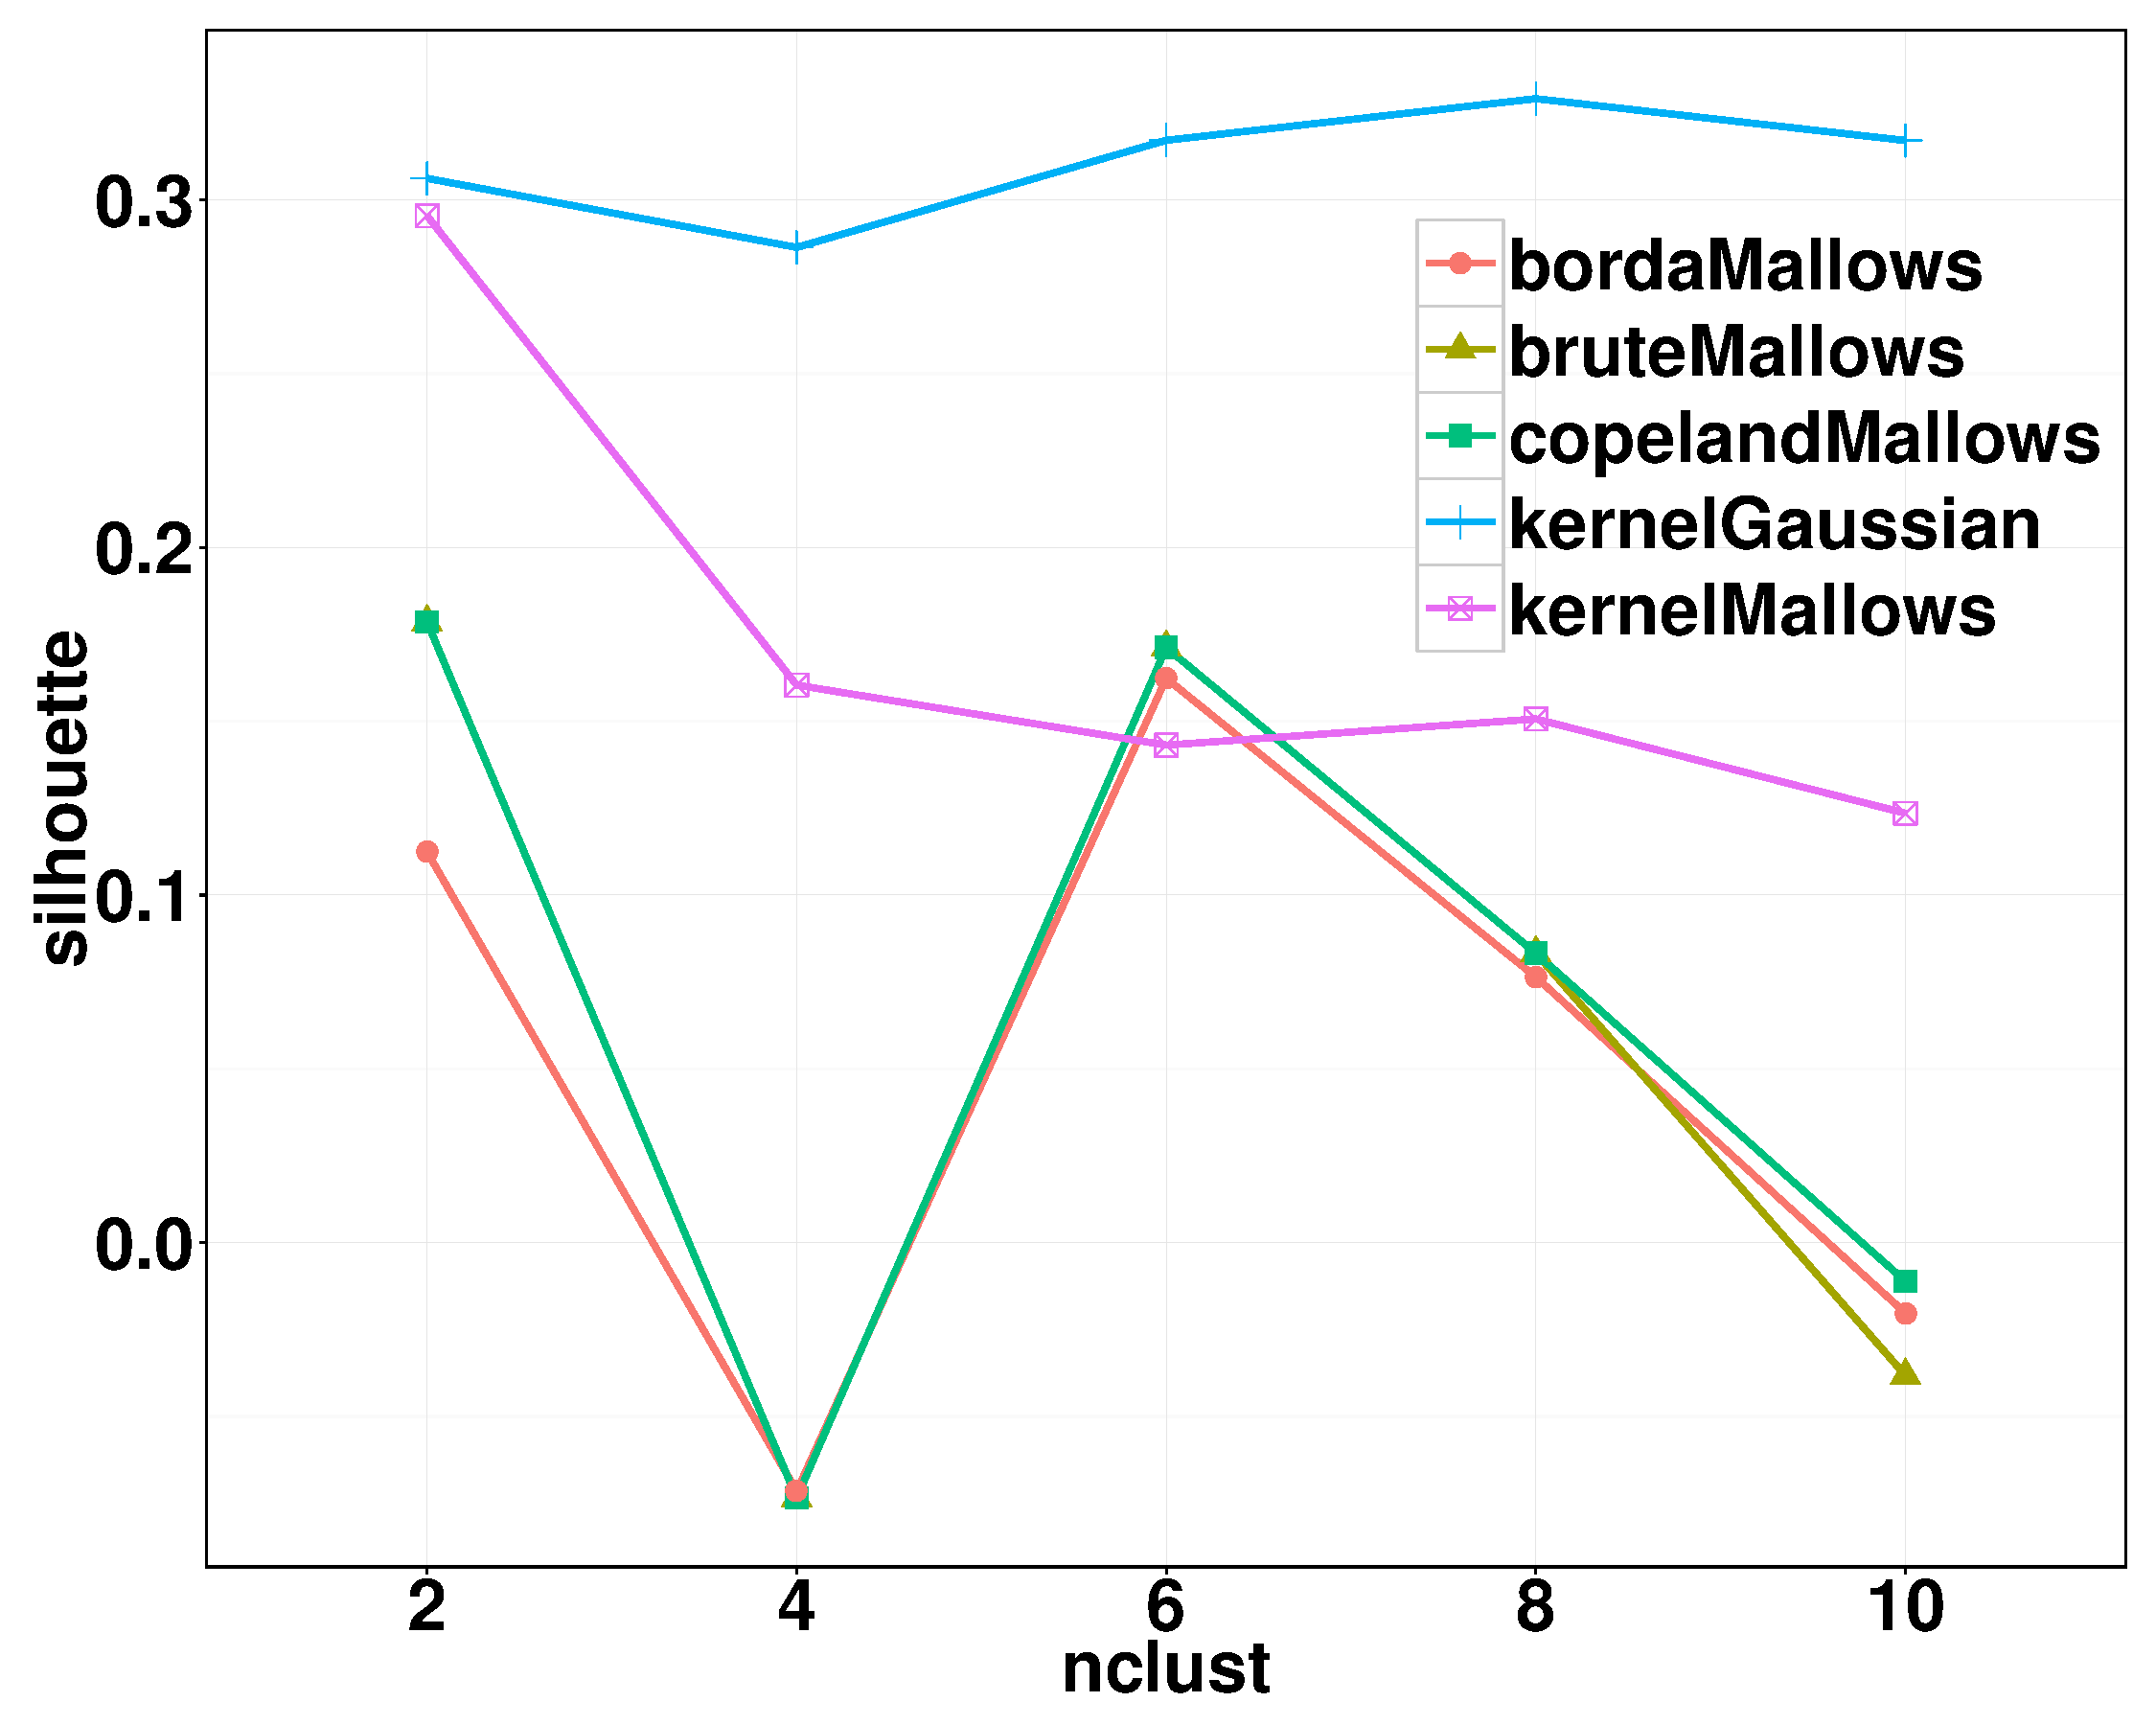
\includegraphics[width=0.6\textwidth]{ch-kendall/cluster_results/mallows-silhouette}
\caption{Average silhouette scores of Mallows mixture modeling methods across different number of clusters.}
\label{fig2:mallows-silhouette}
\end{figure}


\noindent {\bf Clustering ESC voting data.} We finally perform clustering on a dataset of multivariate partial rankings. In the finale of Eurovision Song Contest (ESC), each participating country casts one top-$k$ vote over the finalists who represent their home country. Taken from \cite{Jacques2014Model}, the dataset consists of $34$ multivariate ranking instances, each being a series of $6$ partial votes over top $8$ finalists from 2007 to 2012 respectively.



In comparison with the mixture of Insertion Sorting Rank (ISR) model for clustering multivariate partial rank data proposed by \cite{Jacques2014Model}, we implement the kernel $k$-means algorithm (Algorithm \ref{alg:kernelkmeans}) with the extended Kendall kernel to multivariate rankings \eqref{eq2:multivariate} and equal weights $\mu_j=1/p$ where $p=6$ corresponding to the six contests across years. For each fixed number of clusters, the kernel $k$-means algorithm is repeated $100$ times with randomly initialized configurations while $10$ times for the ISR mixture modeling approach. We vary the number of clusters ranging from $2$ to $6$, and the optimal number is selected to be $2$ for kernel $k$-means with respect to highest average silhouette score while $5$ for the ISR mixture model with respect to highest BIC value. It consumes $2$ hours in total to fit the ISR mixture model in order for clustering while it only takes less than $10$ seconds to form the partition of data with kernel $k$-means. Although it is beyond the scope of this study to further explore the meaningful voting blocs, the colored map of Asia-Europe in terms of clustering results of participating countries to the ESC according to their voting behavior (Figure \ref{fig2:eurovision}, Left) depicts that there exists interesting geographical alliances between countries in the voting data. For example, country-clusters returned by both algorithms present a sign of strong amity within Eastern Europe. Silhouette plots for both algorithms are shown in Figure \ref{fig2:eurovision} (Right). Despite a relatively small number of clusters selected for the kernel $k$-means, the silhouette plot (Figure \ref{fig2:eurovision-kkmeans}, Right) attests that the underlying clusters are well formed. Note that both silhouette plots opt for the same distance used by kernel $k$-means, which may show bias against a clustering scheme based on probabilistic modeling with ISR mixtures. However, the two approaches behave distinctly in identifying subgroups. For example, the ISR mixture model distinguishes Portugal as a singleton among all countries, while interpreting such clustering results remains to be studied. On the other hand, the $k$-means based approach tends to find more evenly distributed subgroups, in the sense that the number of individuals in each subgroup is more consistent. Therefore kernel $k$-means clustering is favored if the study of interest lies in populous behaviors in voting despite of potential outlier individuals. Notably the detection of outliers can be done by other kernel algorithms (Section \ref{sec2:discussion}).

\begin{figure}[!htbp]

\begin{subfigure}{\textwidth}
\centering
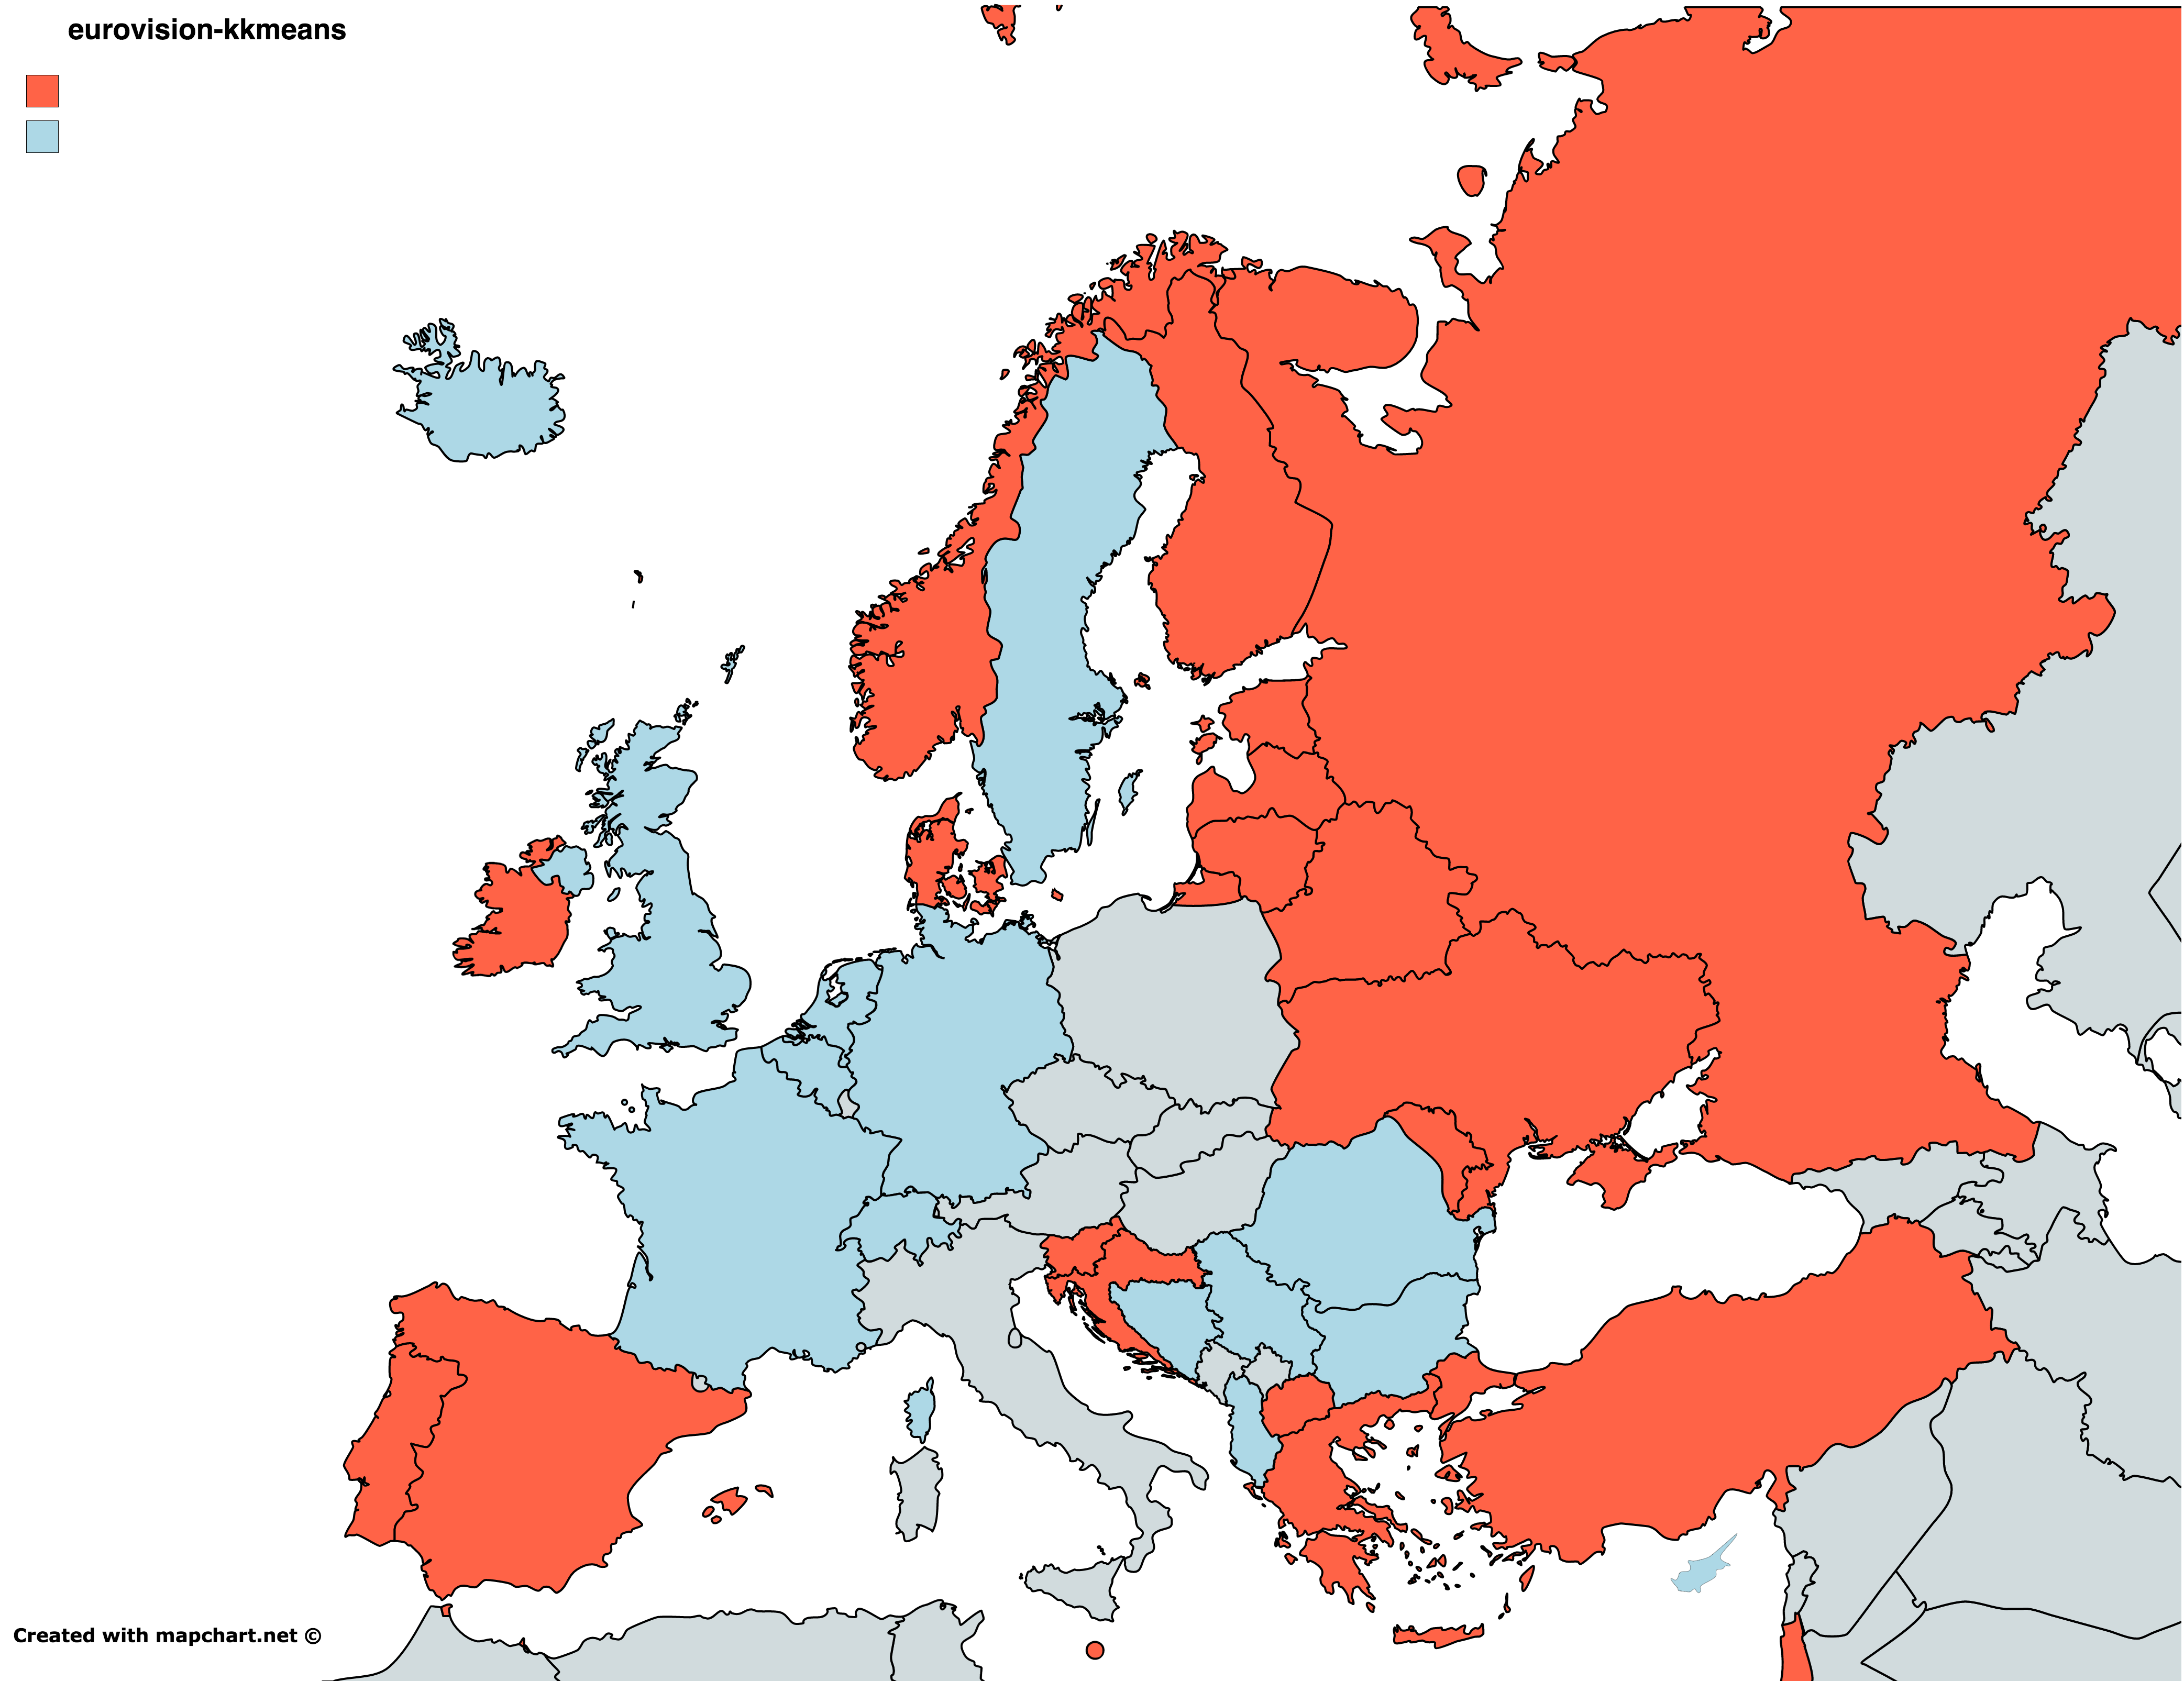
\includegraphics[width=0.45\textwidth]{ch-kendall/cluster_results/eurovision-kkmeans}%
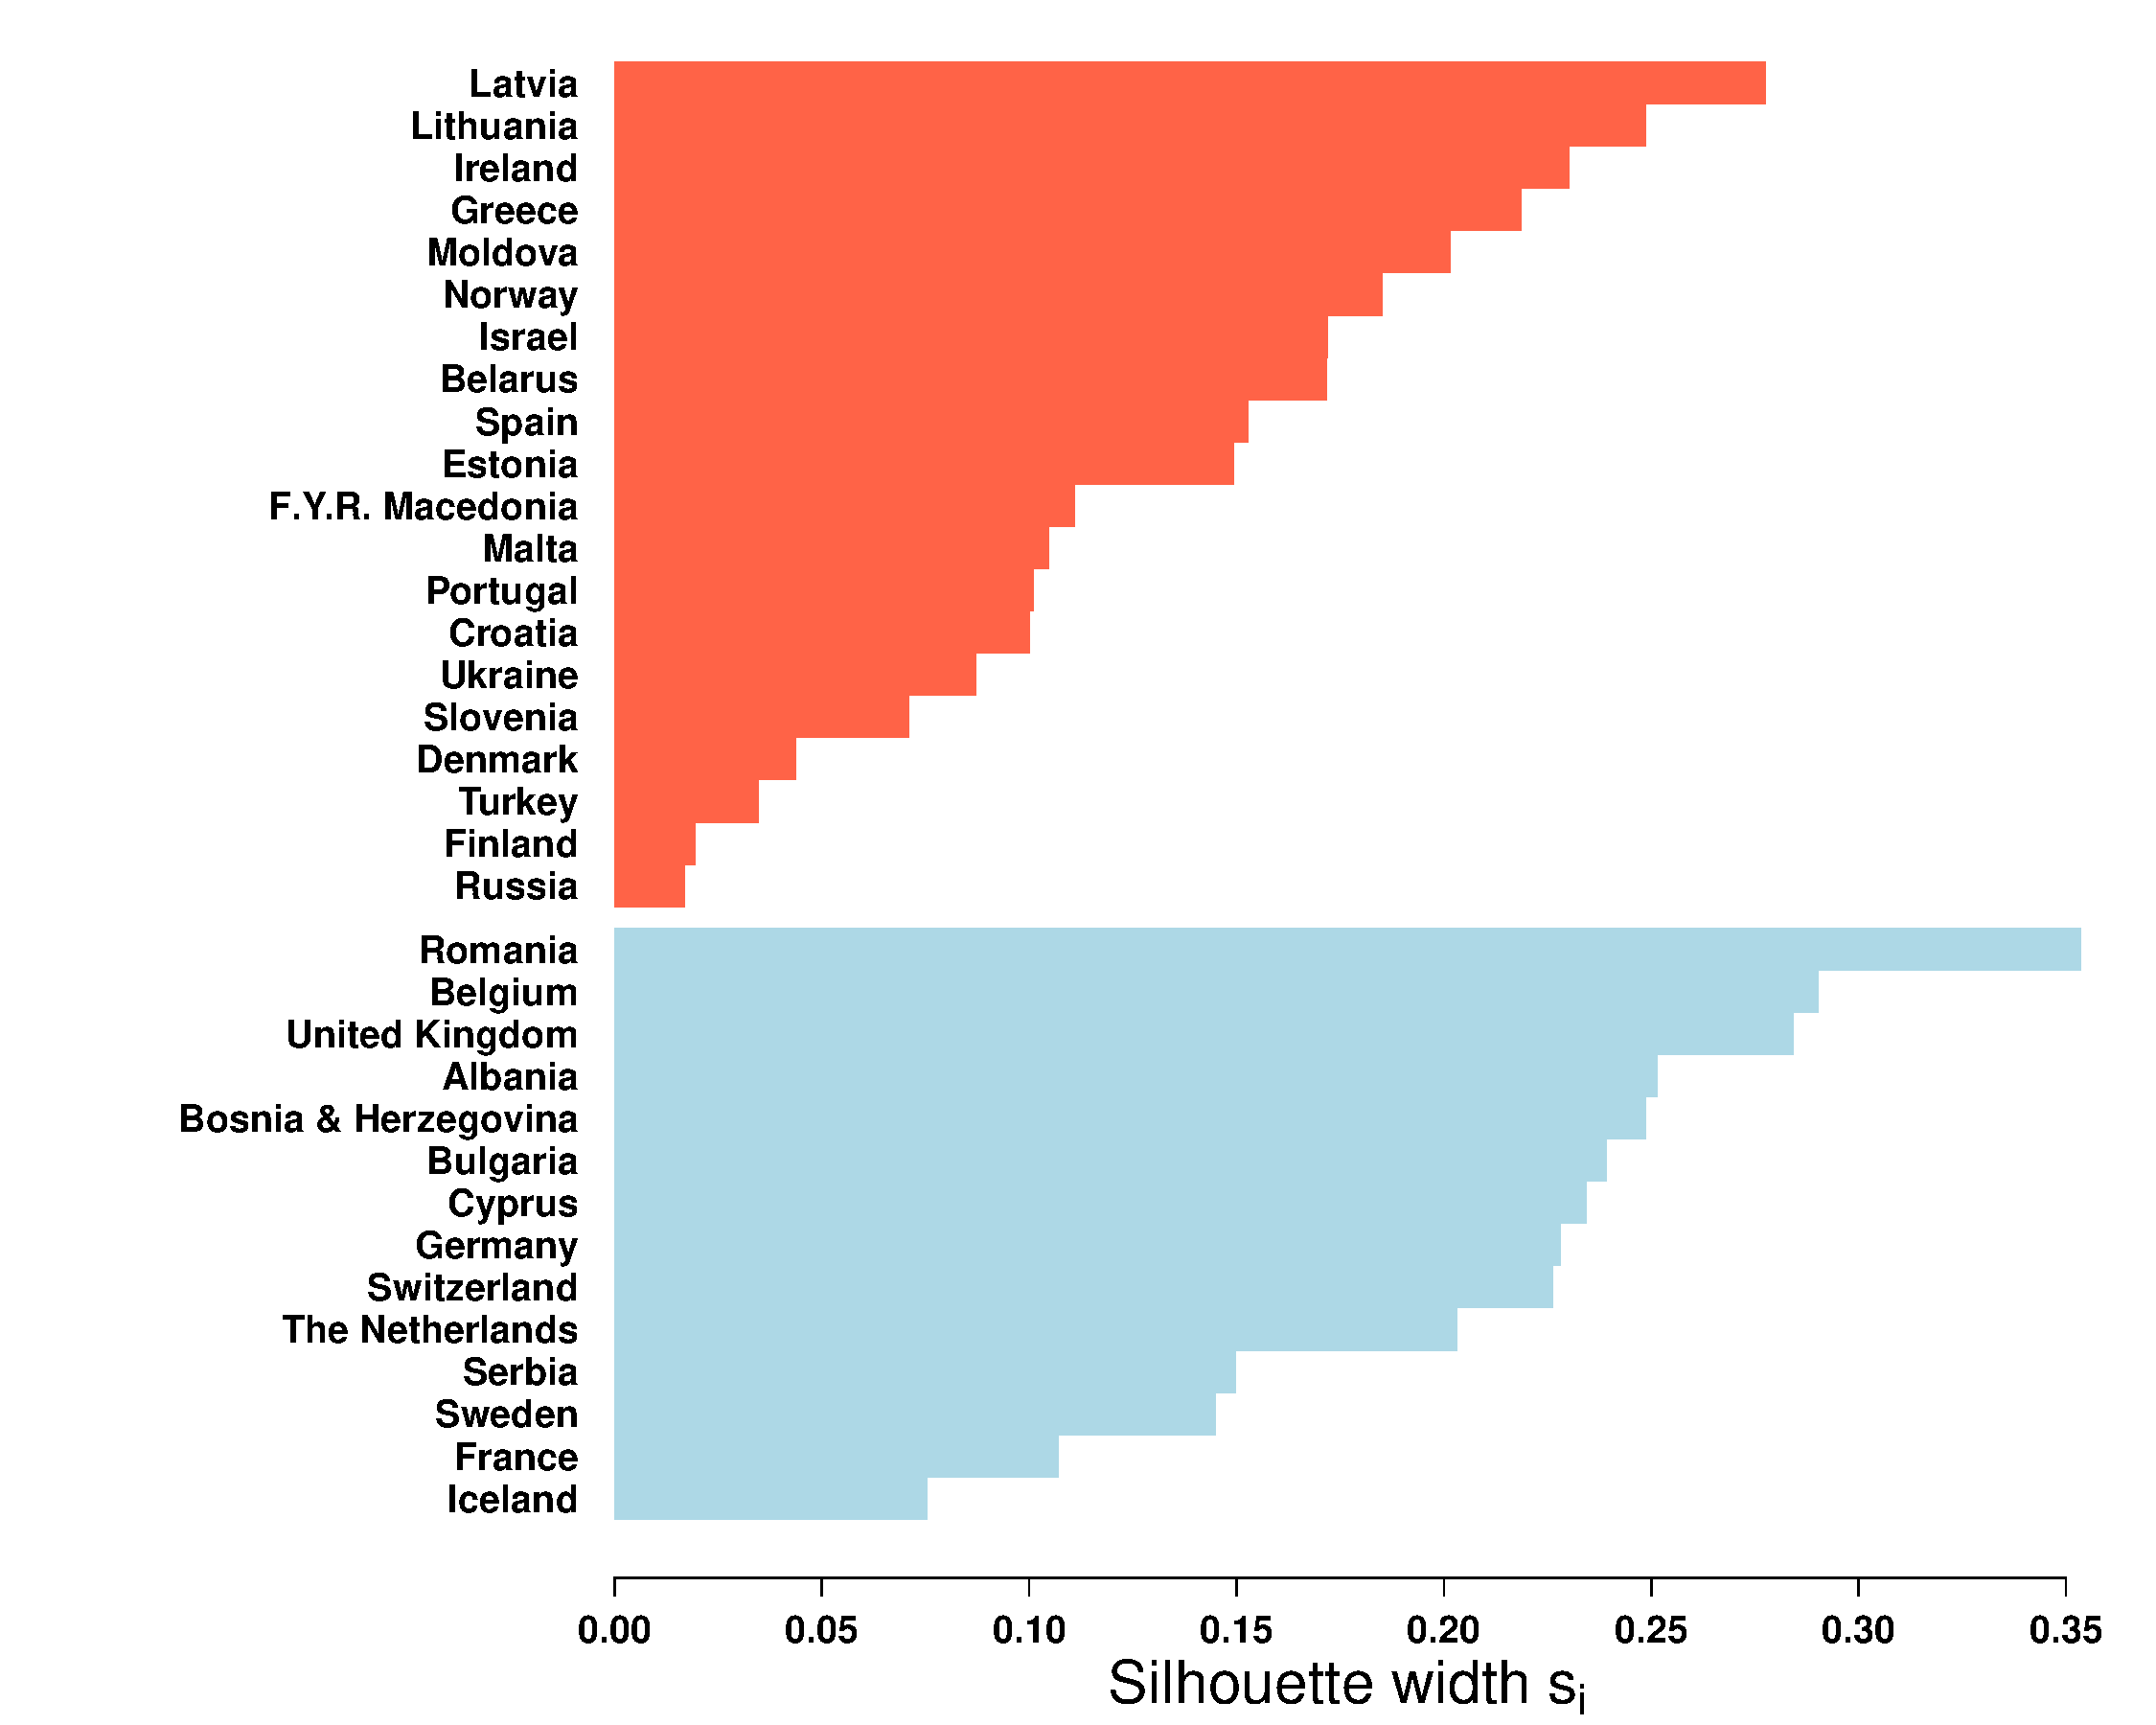
\includegraphics[width=0.45\textwidth]{ch-kendall/cluster_results/eurovision-silhouette-kkmeans}
\caption{Country-clusters returned by kernel $k$-means, where the number of clusters $2$ is selected with respect to highest silhouette score averaged over all countries.}
\label{fig2:eurovision-kkmeans}
\end{subfigure}

\begin{subfigure}{\textwidth}
\centering
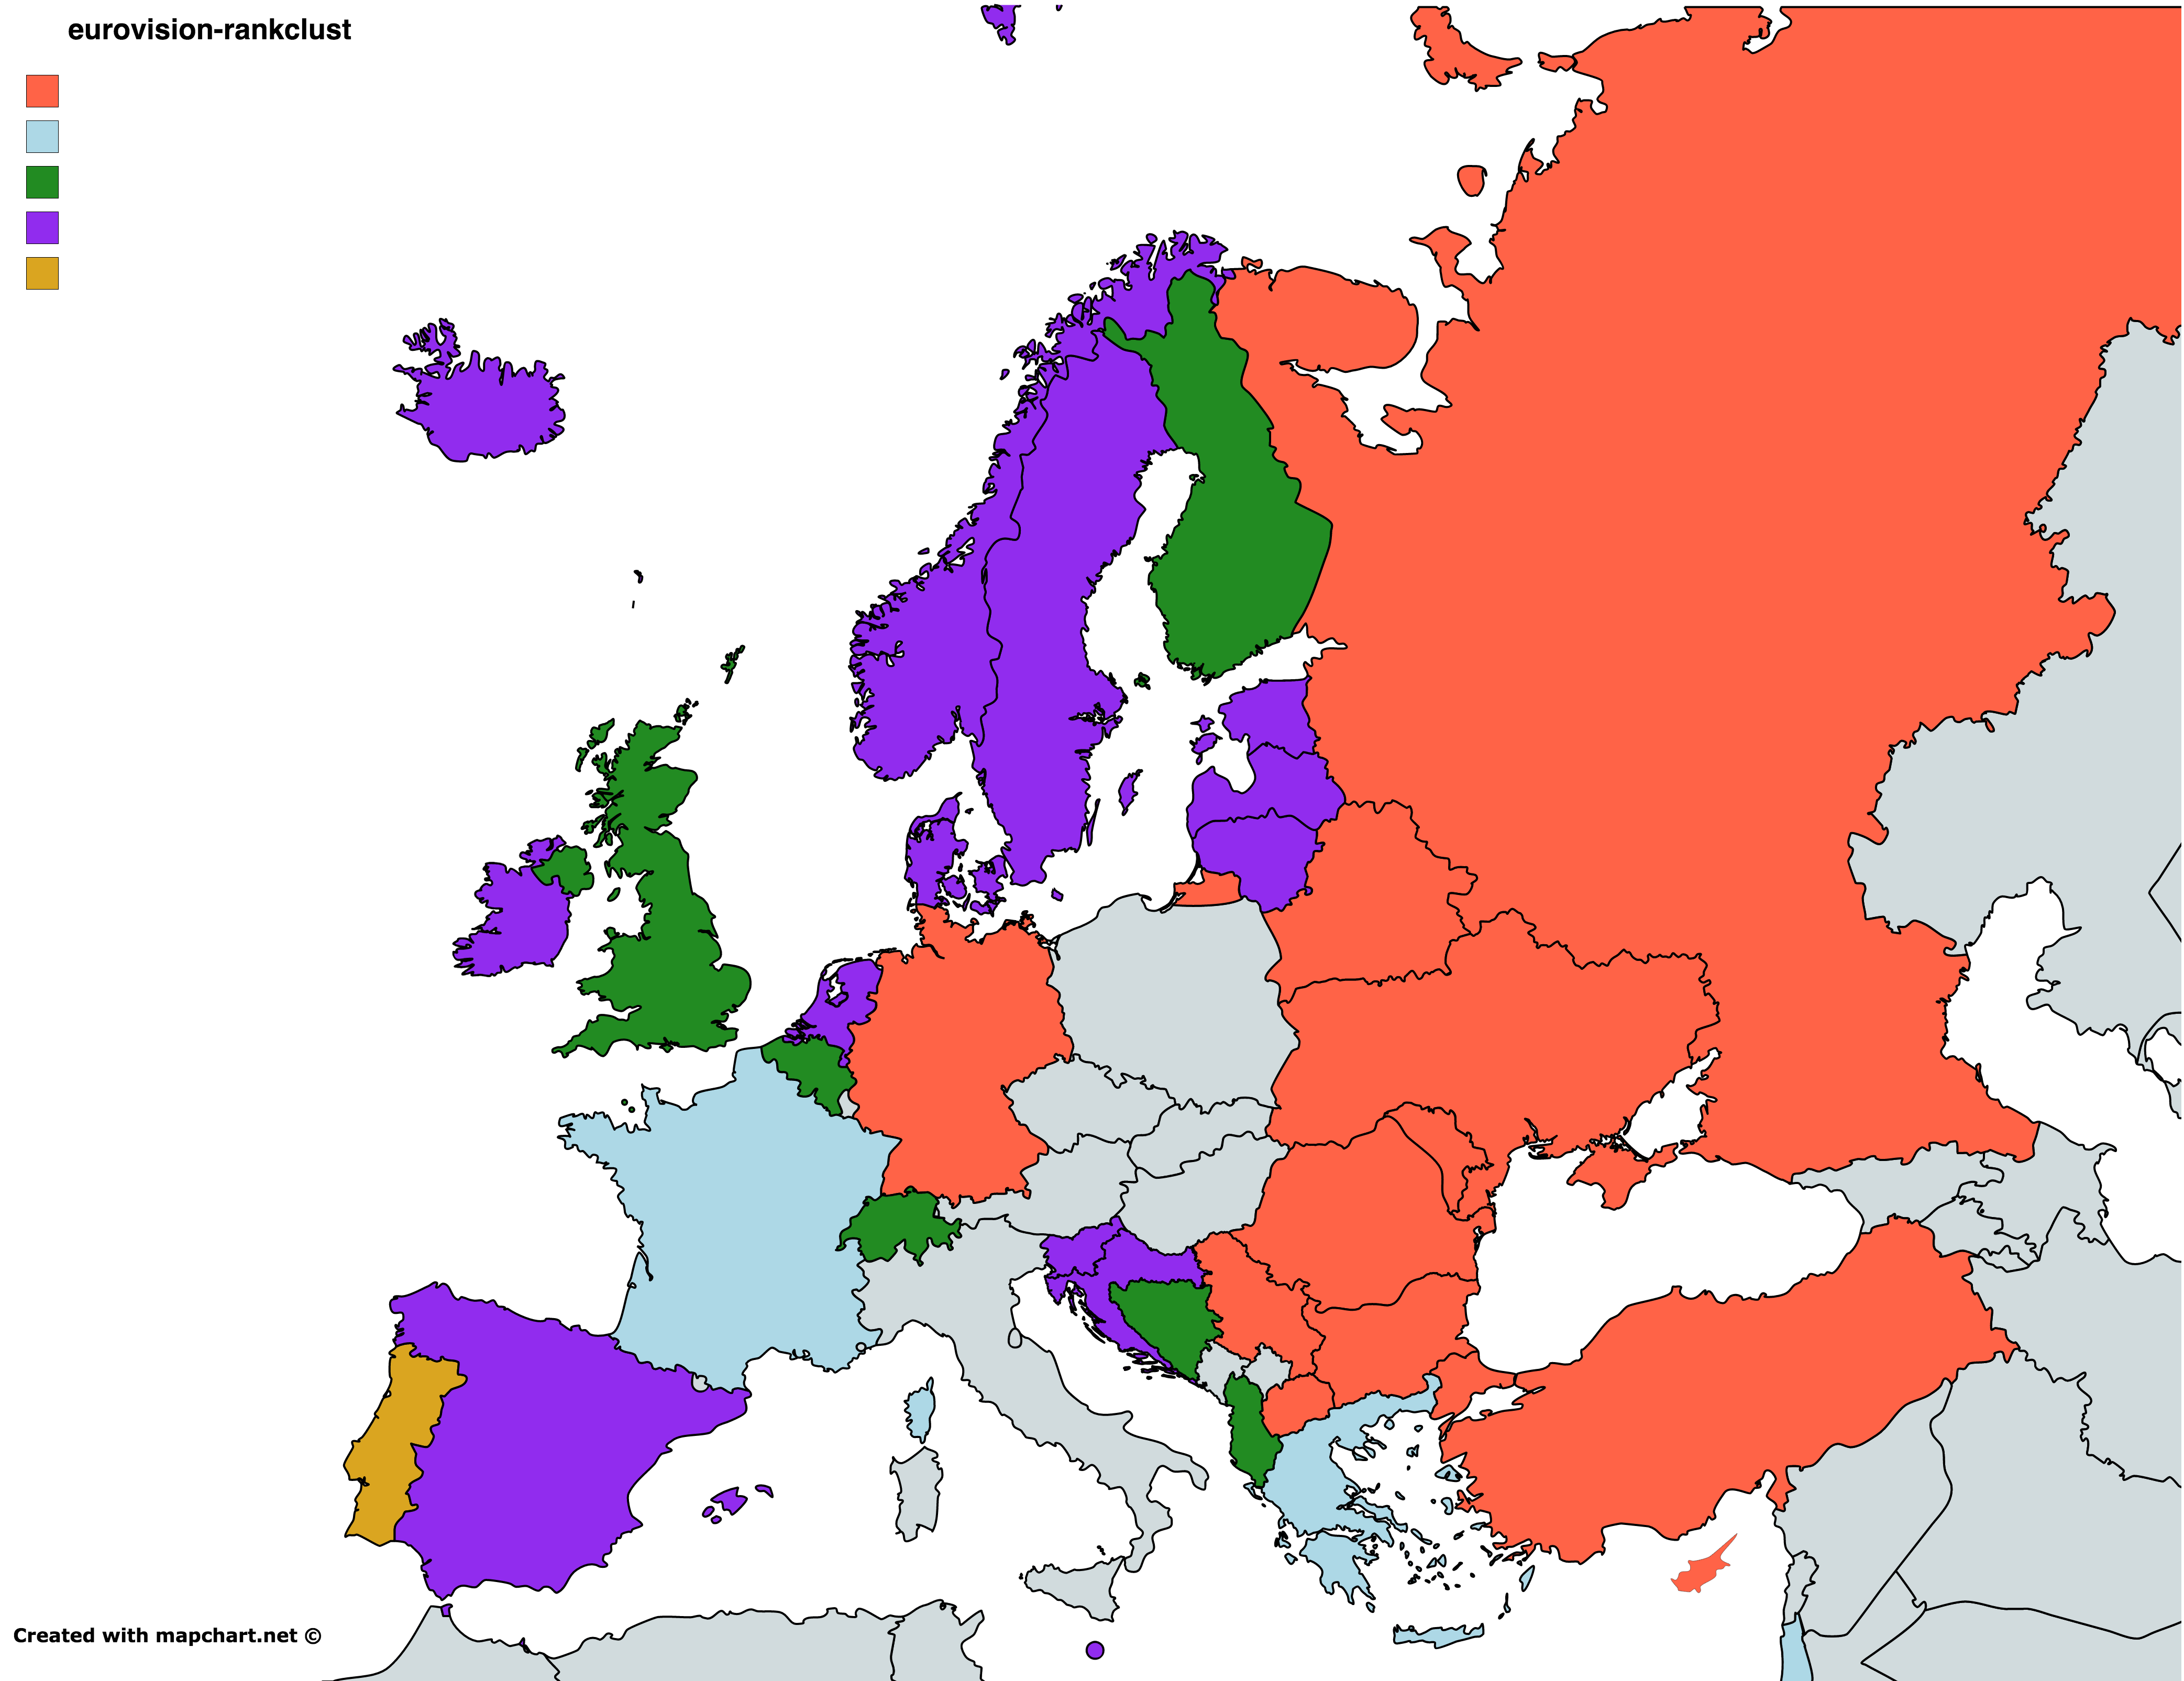
\includegraphics[width=0.45\textwidth]{ch-kendall/cluster_results/eurovision-rankclust}%
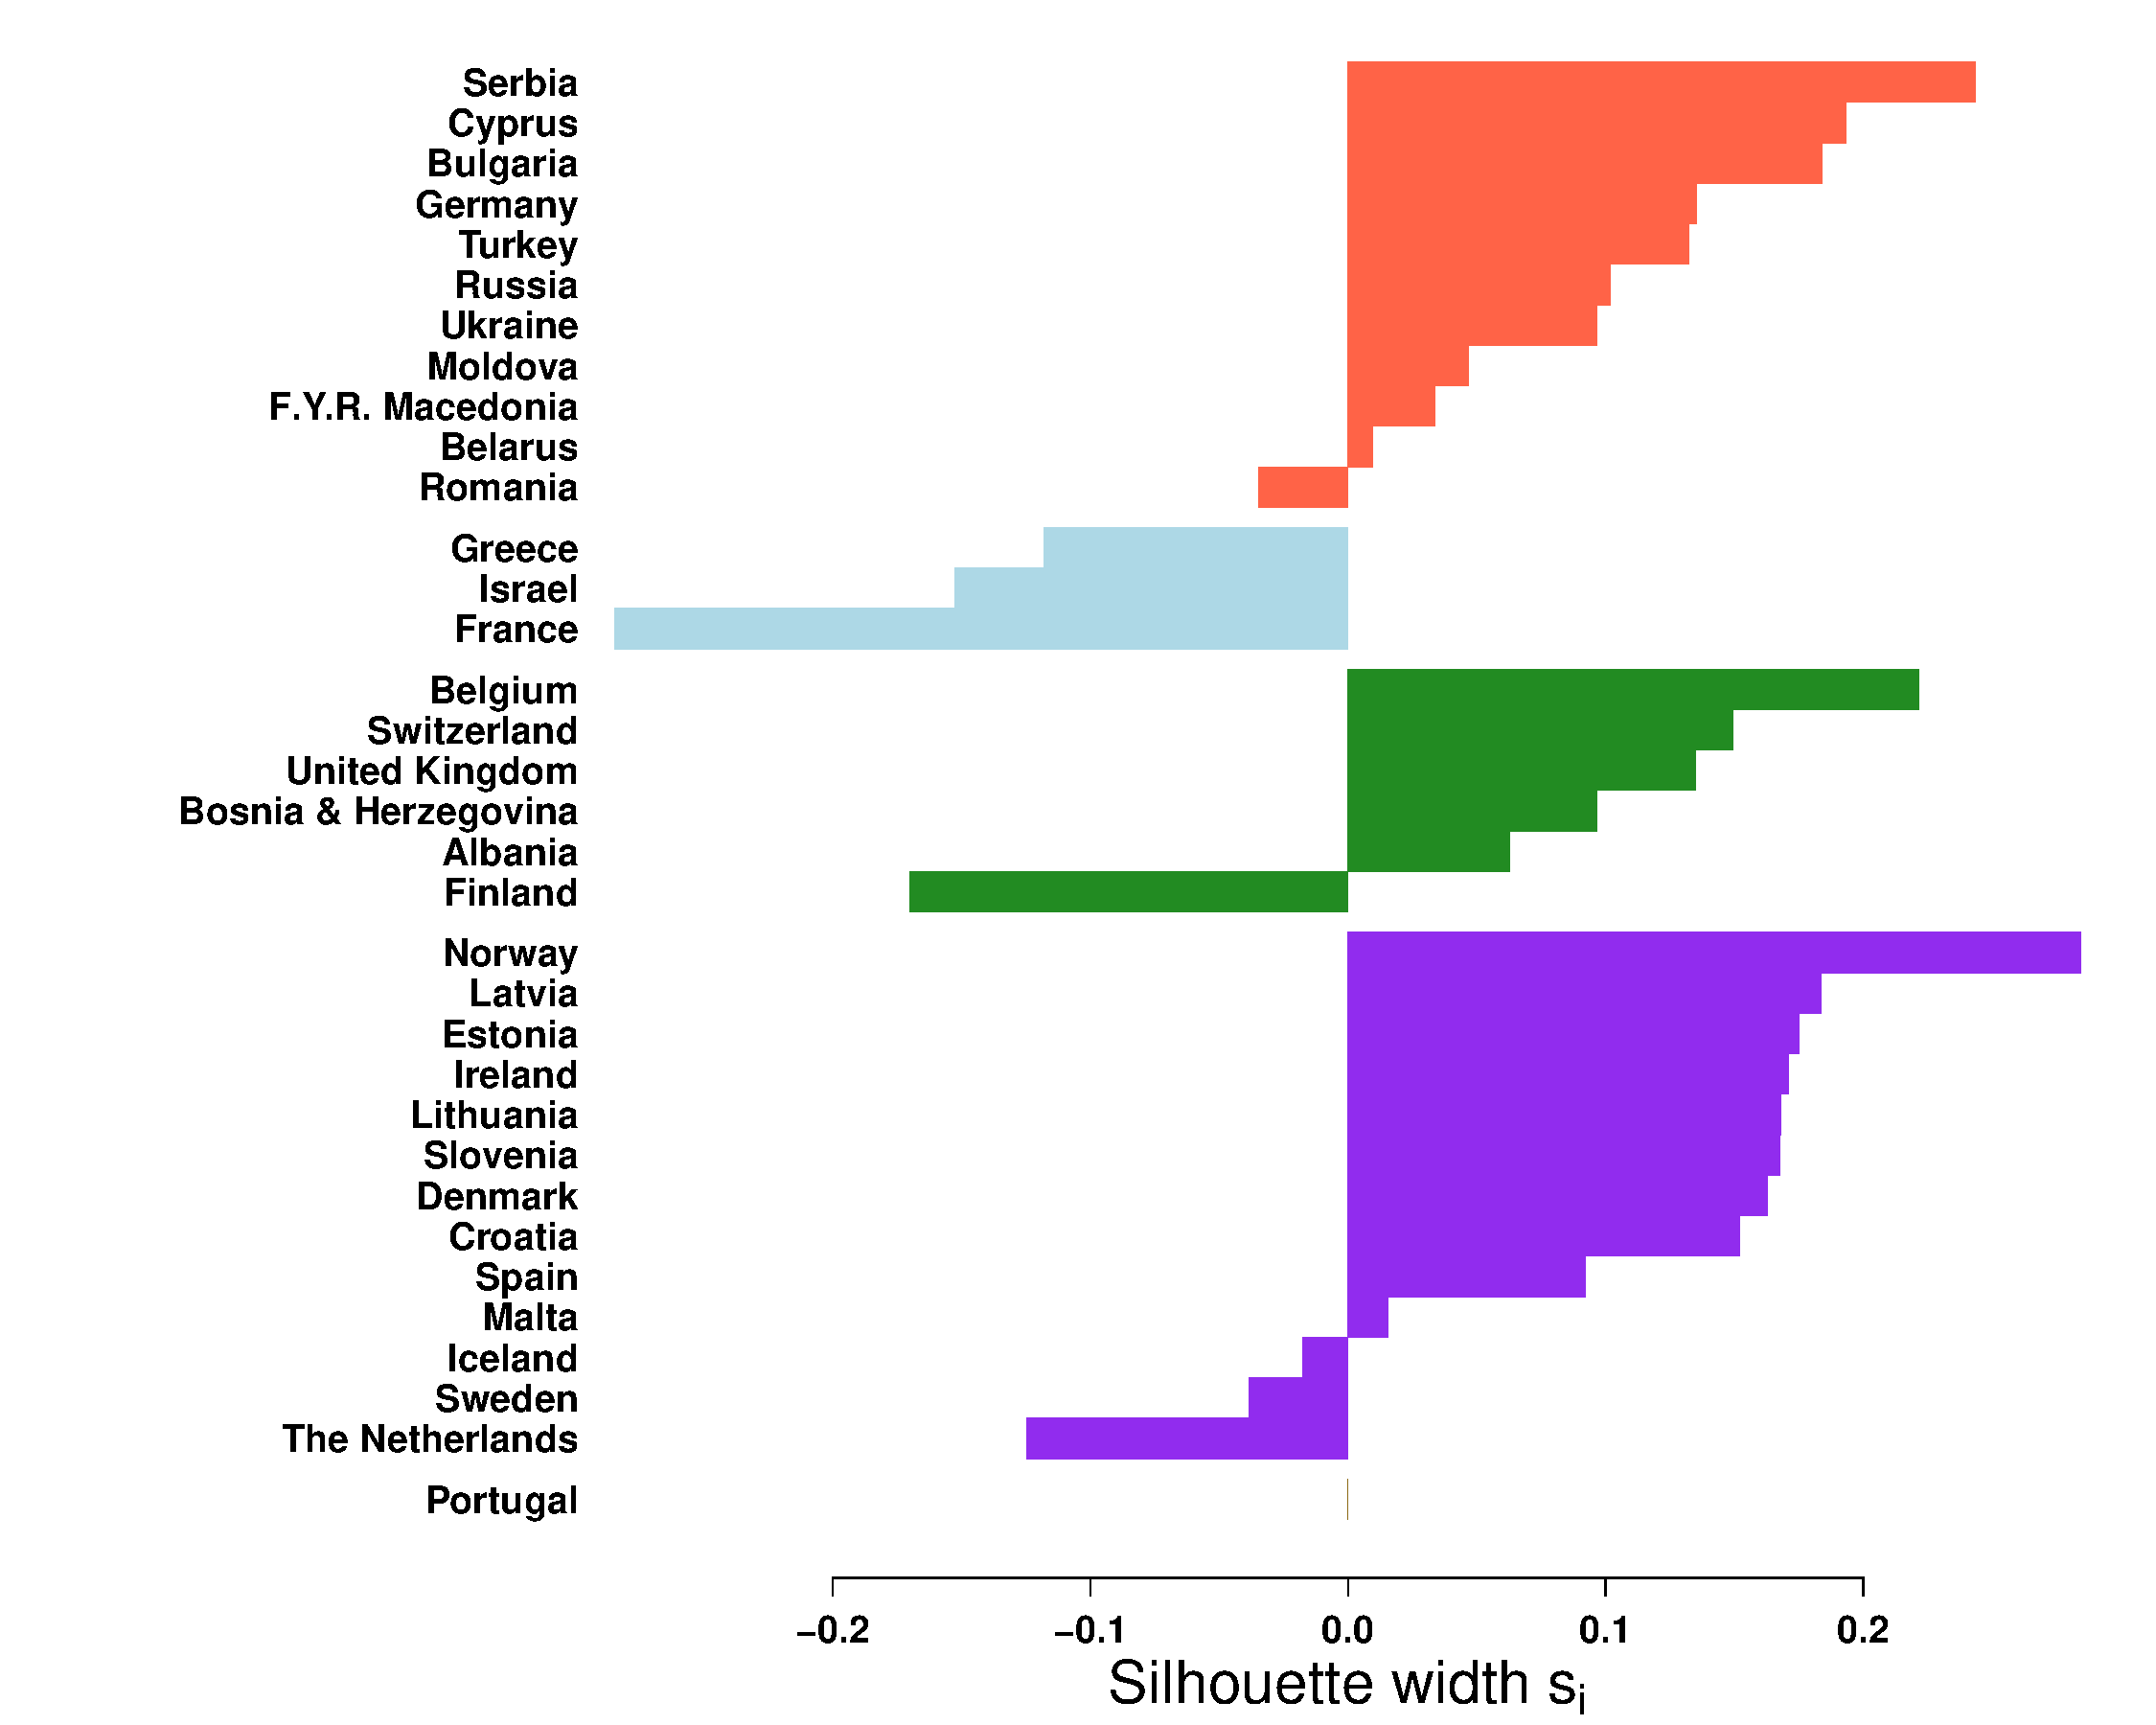
\includegraphics[width=0.45\textwidth]{ch-kendall/cluster_results/eurovision-silhouette-rankclust}
\caption{Country-clusters returned by ISR mixture modeling, where the number of clusters $5$ (including in particular ``Portugal'' as a singleton) is selected with respect to highest fitted BIC value.}
\label{fig2:eurovision-rankclust}
\end{subfigure}

\caption{Clustering results of participating countries to the ESC according to their voting behavior illustrated by geographic map and silhouette plot.}
\label{fig2:eurovision}
\end{figure}



\section{Application: Supervised Classification of Biomedical Data}
\label{sec2:classification}



In this section we illustrate the relevance of supervised classification of rank data with an SVM using the Kendall kernel, when the ranking are derived from a high-dimensional real-valued vector. More precisely, we investigate the performance of classifying high-dimensional biomedical data, motivated by previous work demonstrating the relevance of replacing numerical features by pairwise comparisons in this context \cite{Geman2004Classifying,Tan2005Simple,Xu2005Robust,Lin2009ordering}. 



For that purpose, we collected 10 datasets related to human cancer research publicly available online \cite{Li2003Mean,Schroeder2011breastCancerTRANSBIG,Shi2011Top}, as summarized in Table \ref{tab2:exprdataset}. The features are proteomic spectra relative intensities for the \emph{Ovarian Cancer} dataset and gene expression levels for all the others. The contrasting classes are typically ``Non-relapse v.s. Relapse'' in terms of cancer prognosis, or ``Normal v.s. Tumor'' in terms of cancer identification. The datasets have no missing values, except the \emph{Breast Cancer 1} dataset for which we performed additional preprocessing to remove missing values as follows: first we removed two samples (both labeled ``relapse'') from the training set that have around 10\% and 45\% of missing gene values; next we discarded any gene whose value was missing in at least one sample, amounting to a total of 3.5\% of all genes.


\begin{table}[!htbp]
\caption{Summary of biomedial datasets.}
\label{tab2:exprdataset}
\begin{center}
\begin{scriptsize}
\begin{tabular}{ccccc}
\hline
Dataset & No. of features & \multicolumn{2}{c}{No. of samples (training/test)} & Reference \\
& & $C_1$ & $C_2$ & \\
\hline
Breast Cancer 1 & 23624 & 44/7 (Non-relapse) & 32/12 (Relapse) & \cite{Veer2002Gene} \\
%\hline
Breast Cancer 2 & 22283 & 142 (Non-relapse) & 56 (Relapse) & \cite{Desmedt2007Strong} \\
%\hline
Breast Cancer 3 & 22283 & 71 (Poor Prognosis) & 138 (Good Prognosis) & \cite{Wang2005HykGene} \\
%\hline
Colon Tumor & 2000 & 40 (Tumor) & 22 (Normal) & \cite{Alon1999Broad} \\
%\hline
Lung Adenocarcinoma 1 & 7129 & 24 (Poor Prognosis) & 62 (Good Prognosis) & \cite{Beer2002Gene} \\
%\hline
Lung Cancer 2 & 12533 & 16/134 (ADCA) & 16/15 (MPM) & \cite{Gordon2002Translation} \\
%\hline
Medulloblastoma & 7129 & 39 (Failure) & 21 (Survivor) & \cite{Pomeroy2002Prediction} \\
%\hline
Ovarian Cancer & 15154 & 162 (Cancer) & 91 (Normal) & \cite{Petricoin2002Use} \\
%\hline
Prostate Cancer 1 & 12600 & 50/9 (Normal) & 52/25 (Tumor) & \cite{Singh2002Gene} \\
%\hline
Prostate Cancer 2 & 12600 & 13 (Non-relapse) & 8 (Relapse) & \cite{Singh2002Gene} \\
\hline
\end{tabular}
\end{scriptsize}
\end{center}
\end{table}



We compare the Kendall kernel to three standard kernels, namely linear kernel, homogeneous 2nd-order polynomial kernel and Gaussian RBF kernel with bandwidth set with ``median trick'', using SVM (with regularization parameter $C$) and Kernel Fisher Discriminant (KFD, without tuning parameter) as classifiers. In addition, we include in the benchmark classifiers based on Top Scoring Pairs (TSP) \cite{Geman2004Classifying}, namely (1-)TSP, $k$-TSP \cite{Tan2005Simple}\footnote{While the original $k$-TSP algorithm selects only top $k$ \textit{disjoint} pairs with the constraint that $k$ is \textit{less than} 10, we do not restrict ourselves to any of these two conditions since we consider $k$-TSP in this study essentially a feature pair scoring algorithm.} and APMV (all-pairs majority votes, i.e. ${n \choose 2}$-TSP). Finally we also test SVM with various kernels using as input only top features selected by TSP \cite{Shi2011Top}.

In all experiments, each kernel is centered (on the training set) and scaled to unit norm in the feature space. For KFD-based models, we add $10^{-3}$ on the diagonal of the centered and scaled kernel matrix, as suggested by \cite{Mika1999Fisher}. The Kendall kernel we use in practice is a soft version to \eqref{eq2:kdtALL} in the sense that the extremes $\pm 1$ can still be attained in the presence of ties, specifically we use
\begin{equation*}
	K_{\tau}(\mathbf{x},\mathbf{x}') = \frac{n_c(\mathbf{x},\mathbf{x}')-n_d(\mathbf{x},\mathbf{x}')}{\sqrt{(n_0-n_1)(n_0-n_2)}} \,,
\end{equation*}
where $n_0={n \choose 2}$ and $n_1,n_2$ are the number of tied pairs in $\mathbf{x},\mathbf{x}'$ respectively.

For the three datasets that are split into training and test sets, we report the performance on the test set; otherwise we perform a 5-fold cross-validation repeated 10 times and report the mean performance over the $5\times 10=50$ splits to evaluate the performance of the different methods. In addition, on each training set, an internal 5-fold cross-validation is performed to tune parameters, namely the $C$ parameter of SVM-based models (optimized over a grid ranging from $10^{-2}$ to $10^3$ in $\log$ scale), and the number $k$ of $k$-TSP in case of feature selection (ranging from $1$ to $5000$ in $\log$ scale).




Table \ref{tab2:exprresult} and Figure \ref{fig2:exprresult-acc} summarize the performance of each model across the datasets. An SVM with the Kendall kernel achieves the highest average prediction accuracy overall ($79.39\%$), followed by a linear SVM trained on a subset of features selected from the top scoring pairs ($77.16\%$) and a standard linear SVM ($76.09\%$). The SVM with Kendall kernel outperforms all the other methods at a P-value of $0.07$ according to a Wilcoxon rank test. We note that even though models based on KFD generally are less accurate than those based on SVMs, the relative order of the different kernels is consistent between KFD and SVM, adding evidence that the Kendall kernel provides an interesting alternative to other kernels in this context. The performance of TSP and $k$-TSP, based on majority vote rules, are comparatively worse than SVMs using the same features, as already observed by \cite{Shi2011Top}.



\begin{table}[!htbp]
\caption{Prediction accuracy (\%) of different methods across biomedical datasets. Models are named after candiate methods (SVM or KFD) and candiate kernels, namely linear kernel (linear), 2nd-order homogeneous polynomial kernel (poly), Gaussian RBF kernel (rbf) or Kendall kernel (kdt), and whether feature selection is combined (TOP) or not (ALL).}
\label{tab2:exprresult}
\begin{center}
\begin{scriptsize}
\begin{tabular}{|c|c|cccccccccc|}
\hline
		 & Average & BC1 & BC2 & BC3 & CT & LA1 & LC2 & MB & OC & PC1 & PC2 \\\hline
SVMkdtALL & 79.39 & 78.95 & 71.31 & 67.34 & 85.78 & 70.98 & 97.99 & 63.67 & 99.48 & 100 & 58.4 \\
SVMlinearTOP & 77.16 & 84.21 & 69.29 & 67.11 & 84.19 & 63.92 & 97.32 & 65.17 & 99.41 & 85.29 & 55.7 \\
SVMlinearALL & 76.09 & 78.95 & 71.67 & 64.27 & 86.73 & 70.23 & 97.99 & 62.67 & 99.64 & 73.53 & 55.17 \\
SVMkdtTOP & 75.5 & 52.63 & 70.61 & 65.81 & 85.46 & 67.7 & 97.99 & 58.33 & 99.92 & 97.06 & 59.47 \\
SVMpolyALL & 74.54 & 68.42 & 71.62 & 63.66 & 78.43 & 70.53 & 98.66 & 61.17 & 99.28 & 79.41 & 54.23 \\
KFDkdtALL & 74.33 & 63.16 & 59.41 & 67.22 & 85.46 & 59.08 & 99.33 & 59.33 & 98.73 & 97.06 & 54.57 \\
kTSP & 74.03 & 57.89 & 58.22 & 64.47 & 87.23 & 61.7 & 97.99 & 56 & 99.92 & 100 & 56.83 \\
SVMpolyTOP & 73.99 & 63.16 & 69.44 & 66.26 & 79.14 & 65.98 & 99.33 & 60 & 99.21 & 88.24 & 49.1 \\
KFDlinearALL & 71.81 & 63.16 & 60.43 & 67.52 & 77.26 & 57.24 & 97.99 & 59.5 & 100 & 73.53 & 61.43 \\
KFDpolyALL & 71.39 & 63.16 & 60.48 & 67.38 & 75.1 & 58.52 & 97.99 & 60.33 & 100 & 73.53 & 57.43 \\
TSP & 69.71 & 68.42 & 49.58 & 57.8 & 85.61 & 58.96 & 95.97 & 52.67 & 99.8 & 76.47 & 51.83 \\
SVMrbfALL & 69.31 & 63.16 & 71.41 & 65.87 & 81.18 & 70.84 & 93.96 & 63.83 & 98.85 & 26.47 & 57.5 \\
KFDrbfALL & 66.5 & 63.16 & 60.38 & 66.17 & 84.33 & 58.62 & 97.32 & 60.17 & 98.34 & 26.47 & 50 \\
APMV & 61.91 & 84.21 & 65.98 & 33.96 & 64.49 & 33.6 & 89.93 & 42.17 & 85.19 & 73.53 & 46 \\\hline
\end{tabular}
\end{scriptsize}
\end{center}
\end{table}



\begin{figure}[!htbp]
\begin{center}

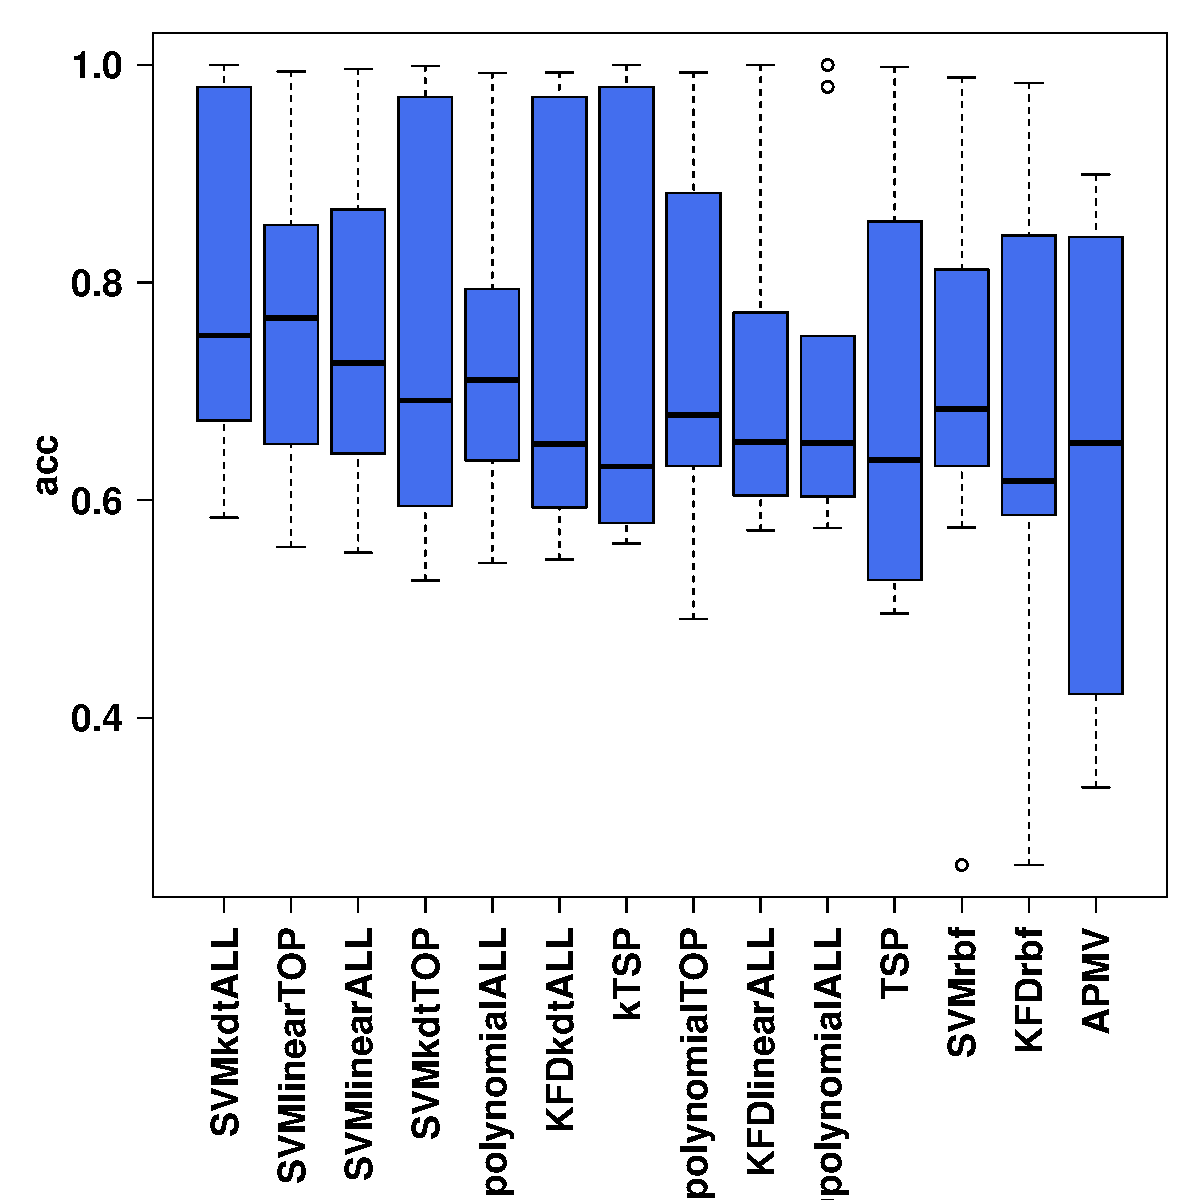
\includegraphics[width=0.6\textwidth]{ch-kendall/clasf_results/acc_plot}
\
\end{center}
\caption{Model performance comparison (ordered by decreasing average accuracy across datasets).}
\label{fig2:exprresult-acc}
\end{figure}




We further studied how the performance of different kernels depends on the choice of the $C$ parameter or the SVM (Figure \ref{fig2:exprresult-perfSVM}), and on the number of features used (Figure \ref{fig2:exprresult-perfFS}), on some representative datasets. We observe that compared to other kernels, an SVM with the Kendall kernel is relatively insensitive to hyper-parameter $C$ especially when $C$ is large, which corresponds to a hard-margin SVM. This may explain in part the success of SVMs in this setting, since the risk of choosing a bad $C$ during training is reduced. Regarding the number of features used in case of feature selection, we notice that it does not seem to be beneficial to perform feature selection in this problem, explaining why the Kendall kernel which uses all pairwise comparisons between features outperforms other kernels restricted to a subset of these pairs. In particular, the feature space of the Kendall and Mallows kernels is precisely the space of binary pairwise comparisons defined by \cite{Geman2004Classifying}, and the results show that instead of selecting a few features in this space as the Top Scoring Pairs (TSP)-family classifiers do \cite{Geman2004Classifying, Tan2005Simple, Xu2005Robust, Lin2009ordering}, one can simply work with \emph{all} pairs with the kernel trick.


\begin{figure}[!htbp]
\begin{center}

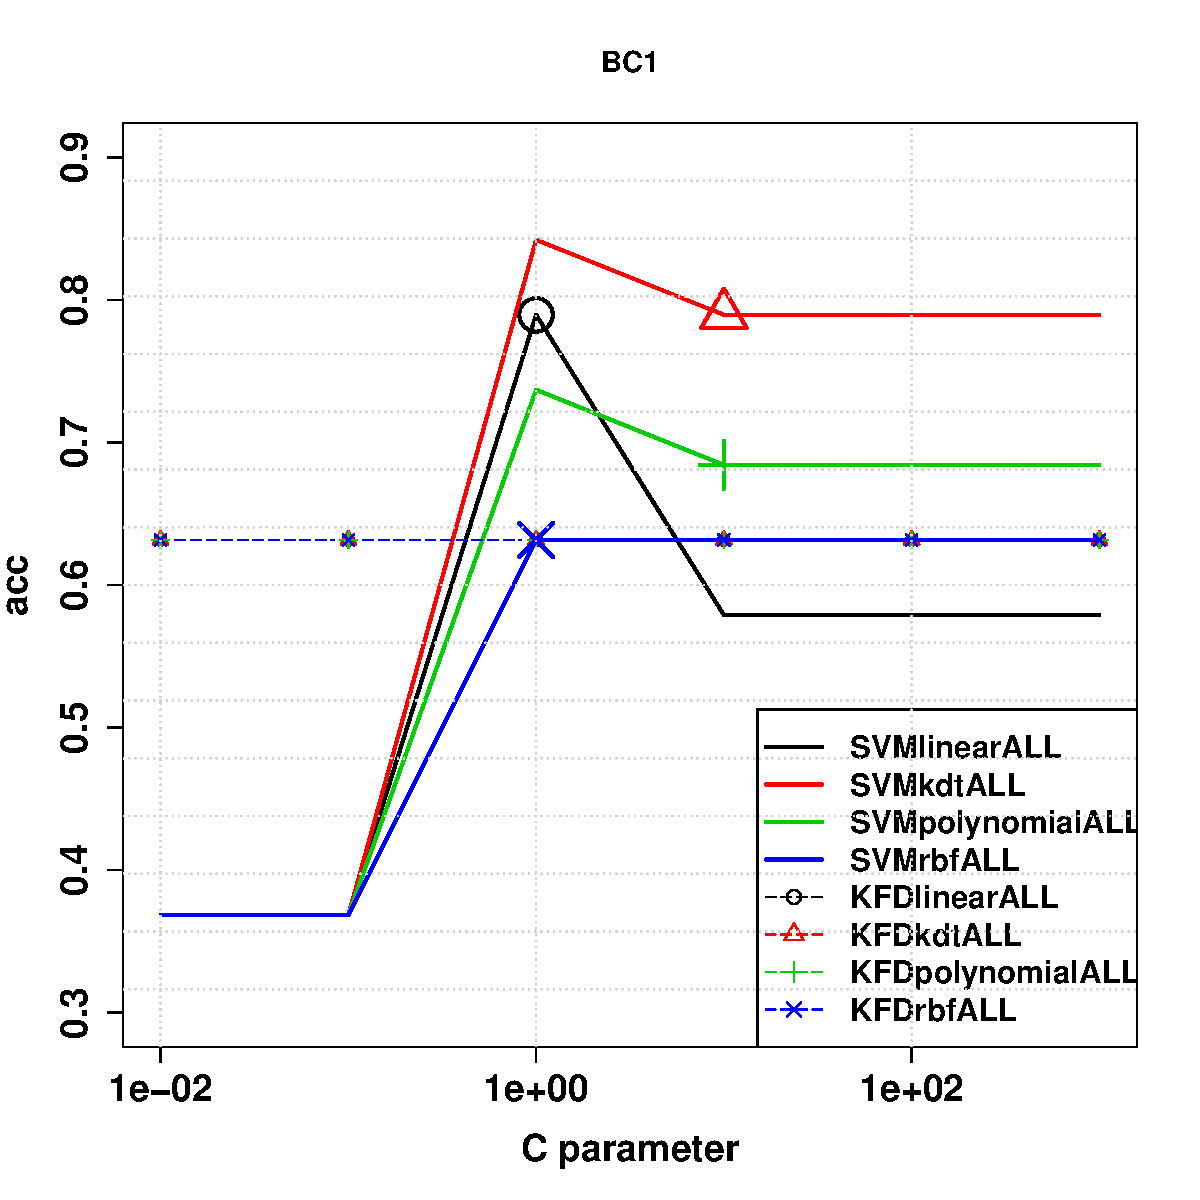
\includegraphics[width=0.6\textwidth]{ch-kendall/clasf_results/acc_perfSVM}

\end{center}
\caption{Sensitivity of kernel SVMs to $C$ parameter on the \emph{Breast Cancer 1} dataset. (Special marks on SVM lines denote the parameter returned by cross-validation.)}
\label{fig2:exprresult-perfSVM}
\end{figure}

\begin{figure}[!htbp]
\begin{center}

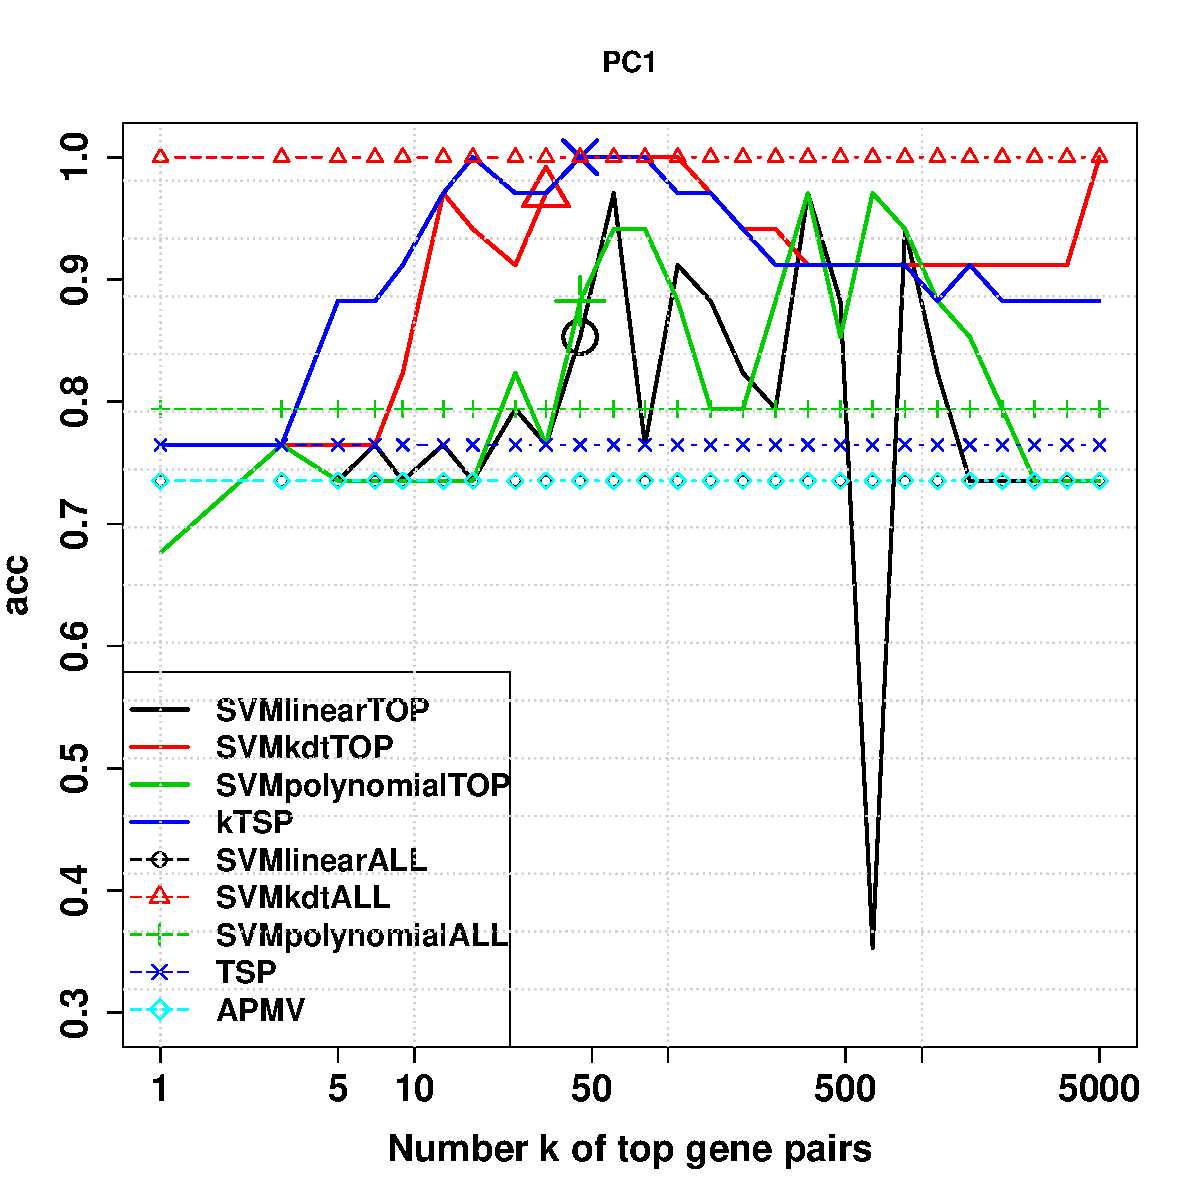
\includegraphics[width=0.6\textwidth]{ch-kendall/clasf_results/acc_perfFS}

\end{center}
\caption{Impact of TSP feature selection on the \emph{Prostate Cancer 1} dataset. (Special marks on SVM lines denote the parameter returned by cross-validation.)}
\label{fig2:exprresult-perfFS}
\end{figure}




Finally, as a proof of concept we empirically compare on one dataset the smooth alternative \eqref{eq2:G} and its Monte Carlo approximate \eqref{eq2:mc} with the original Kendall kernel. We studied how the performance varies with the amount of noise added to the samples (Figure \ref{fig2:exprapprox-stab}), and how the performance varies with the number of samples in the Monte Carlo scheme for a given amount of noise (Figure \ref{fig2:exprapprox-approxsingle}). It confirms that the smooth alternative \eqref{eq2:G} can improve the performance of the Kendall kernel, and that the amount of noise (window size) should be considered as a parameter of the kernel to be optimized. Although the $D^2$-sample Monte Carlo approximate kernel \eqref{eq2:mc} mainly serves as a fast estimate to the exact evaluation of \eqref{eq2:G}, it shows that the idea of jittered input with specific noise can also bring a tempting benefit for data analysis with Kendall kernel, even when $D$ is small. This also justifies the motivation of our proposed smooth alternative \eqref{eq2:G}. Last but not least, despite the fact that the convergence rate of $D^2$-sample Monte Carlo approximate to the exact kernel evaluation is guaranteed by Theorem \ref{thm2:approx}, experiments show that the convergence in practice is typically faster than the theoretical bound, and even faster in case that the window size $a$ is small. This is due to the fact that the convergence rate is also dependent of the observed data distribution in the input space, for which we have not made any specific assumption in our analysis.





\begin{figure}[!htbp]
\begin{center}
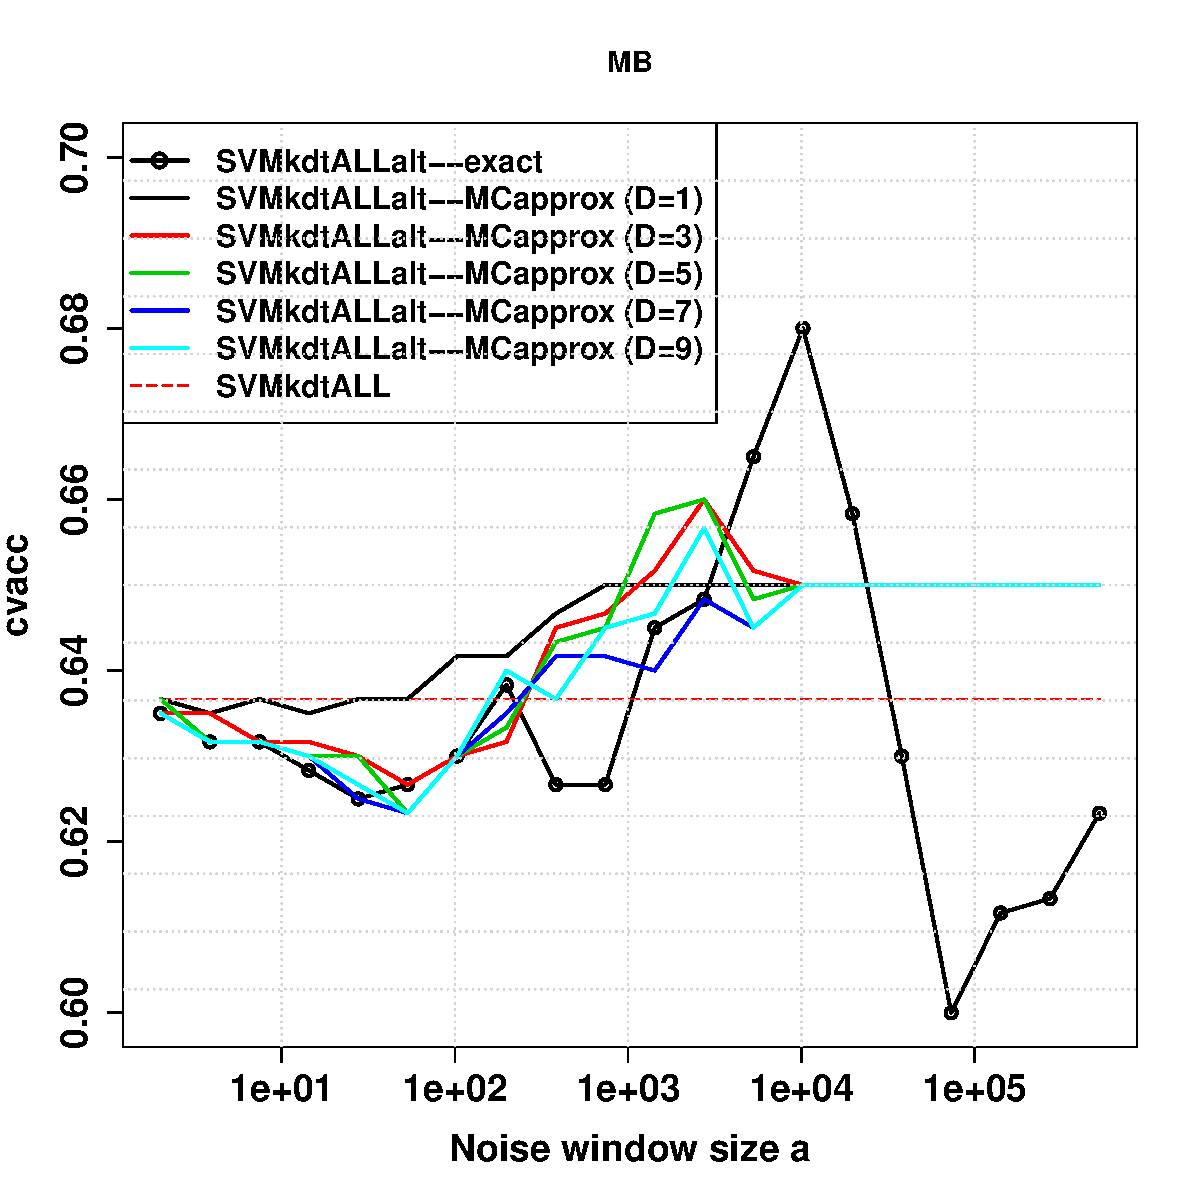
\includegraphics[width=0.6\textwidth]{ch-kendall/clasf_results/acc_StabApprox}
\end{center}
\caption{Empirical performance of smoothed alternative to Kendall kernel on the \emph{Medulloblastoma} dataset.}
\label{fig2:exprapprox-stab}
\end{figure}


\begin{figure}[!htbp]
\begin{center}
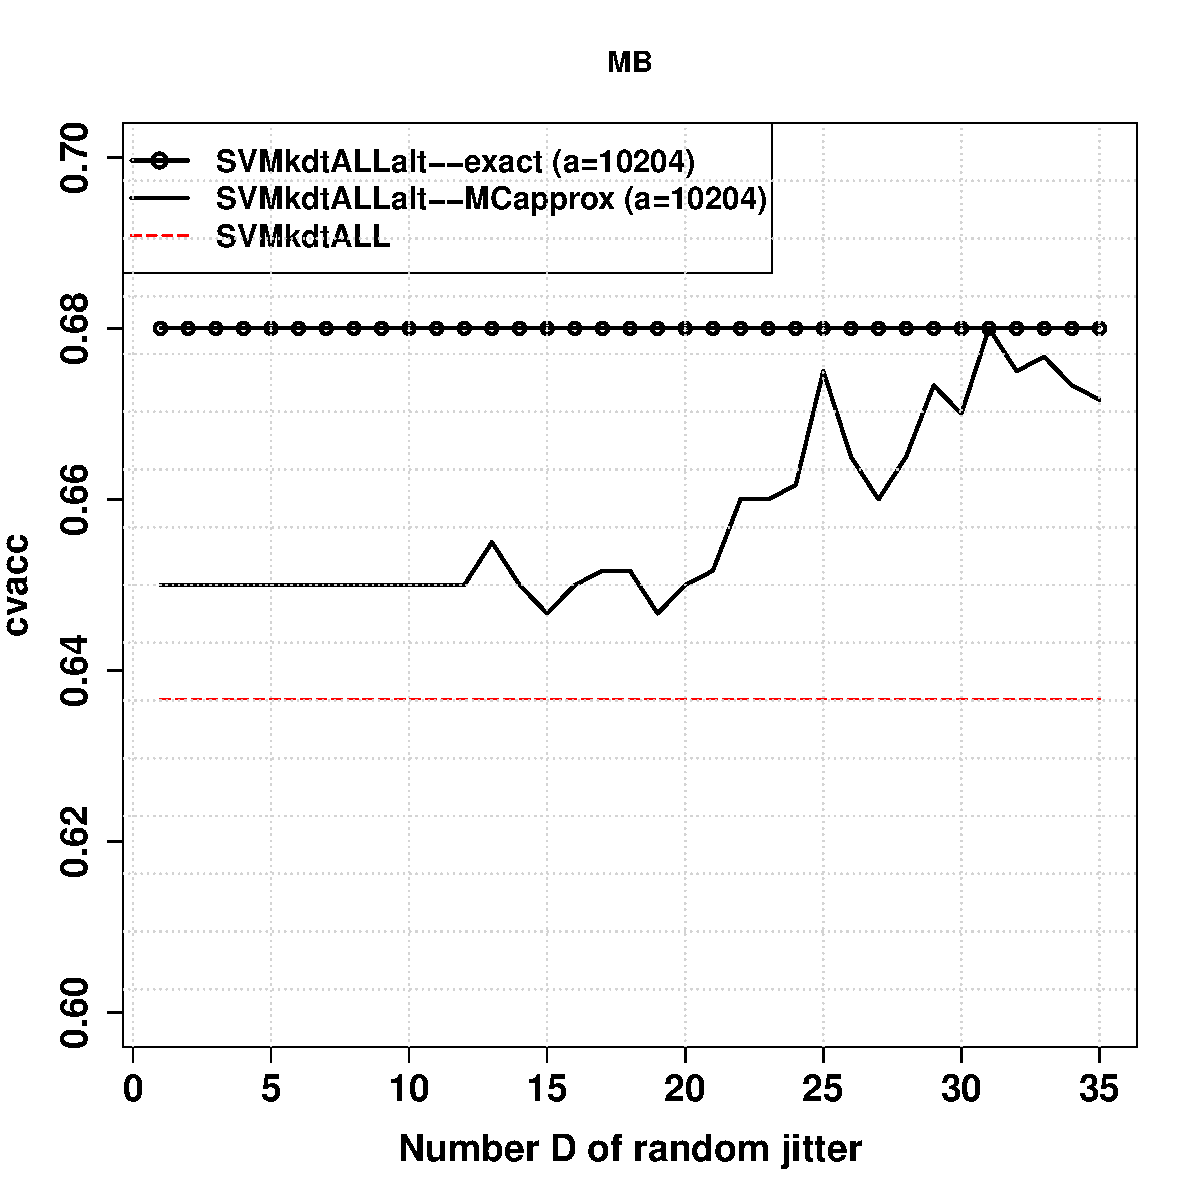
\includegraphics[width=0.6\textwidth]{ch-kendall/clasf_results/acc_approxSingleWindow}
\end{center}
\caption{Empirical convergence of Monte Carlo approximate at the fixed window size attaining maximum underlying accuracy from the left plot.}
\label{fig2:exprapprox-approxsingle}
\end{figure}




\section{Discussion}
\label{sec2:discussion}

Based on the observation that the popular Kendall tau correlation between total rankings is a positive definite kernel, we presented some extensions and applications pertaining to learning with the Kendall kernel and the related Mallows kernel. We showed that both kernels can be evaluated efficiently in $O(n \log n)$ time, and that the Kendall kernel can be extended to partial rankings containing $k$ items out of $n$ in $O(k \log k)$ time as well as to multivariate rankings. When permutations are obtained by sorting real-valued vectors, we proposed an extension of the Kendall kernel based on random perturbations of the input vector to increase its robustness to small variations, and discussed two possible algorithms to compute it. We further highlighted a connection between the fast Mallow kernel and the diffusion kernel of \cite{Kondor2010Ranking}. We also reported promising experimental results on clustering of heterogeneous rank data and classifying biomedical data demonstrating that for highly noisy data, the Kendall kernel is competitive or even outperforms other state-of-the-art kernels. 

We believe that computationally efficient kernels over the symmetric group pave the way to numerous applications beyond the ones we pursued in this chapter. In unsupervised data mining, kernel density estimation for example can be applied to modeling the distribution over a collection of rankings, and by the representer theorem the resulting distribution depends solely on the observed data points circumventing the exponentially large cardinality of the symmetric group, from which a consensus ranking that best represents the data is the one with the highest probability. As more complicated cases, there is much interest beyond finding a single consensus ranking typically in the context of political votes or social choices: groups of homogeneous sub-populations in data can be clustered by algorithms such as kernel $k$-means or spectral clustering \cite{Filippone2008survey}; dependencies or principle structural factors in data can be found by kernel canonical correlation analysis \cite{Lai2000Kernel} or kernel principle component analysis \cite{Schoelkopf1999Kernel}; outliers in a collection of rank data can be detected with one-class SVMs \cite{Schoelkopf1999Support,Tax2004Support}. In a more predictive setting, Support Vector Machines and kernel ridge regression are representative delegates for solving classification and regression problems amongst many other kernel algorithms \cite{Schoelkopf2002Learning}. Notably, the input/output kernels formalism allows us to predict rankings as well as learn from rankings where a wealth of algorithms such as multi-class SVMs or structural SVMs \cite{Crammer2002algorithmic,Tsochantaridis2005Large,Bakir2007Predicting} are ready to suit the problem at hand.

Deeper understanding of the Kendall and Mallows kernels calls for more theoretical work of the proposed kernels. In particular, a detailed analysis of the Fourier spectra of the Kendall and Mallows kernels is provided in \cite{Mania2016Universality}. Those authors also introduced a tractable family of normalized polynomial kernels of degree $p$ that interpolates between Kendall (degree one) and Mallows (infinite degree) kernels.

There are many interesting extensions of the current work. One direction would be to include high-order comparisons in measuring the similarity between permutations. Since the fast computation of the Kendall and Mallows kernels is balanced by the fact that they only rely on pairwise statistics between the ranks, computationally tractable extension to higher-order statistics, such as three-way comparisons, could potentially enhance the discriminative power of the proposed kernels. Another interesting direction would be to extend the proposed kernels to rankings on partially ordered set. In fact, the current work lies on the assumption that a (strict) total order can be associated with the (finite) set of items given to rank $\{x_1,\dots,x_n\}$, which is implicitly presumed when we label the items by the subscripts $\n$ and then define the Kendall and Mallows kernels by comparing all item pairs $(i,j)$ for $i<j$ (Section \ref{sec2:kernel}). However, there are cases when the item set is intrinsically associated with a (strict) partial order such that some item pairs are conceptually incomparable. In that case, we can collect all comparable item pairs into a set denoted by $E$ and define the kernels by comparing only those item pairs $(i,j)$ in $E$. Notably evaluating the extended kernels is still fast as we can simply replace the Merge Sort algorithm for total orders (Section \ref{sec2:kernel}) by a topological sort algorithm for partial orders \cite[Section 22.4]{Cormen2009Introduction}. We leave further investigations of this generalization to future work.


\cleardoublepage

\chapter{Network-based Wavelet Smoothing for Analysis of Genomic Data}
\label{chap:wavelet}

\begin{chapabstract}{Publication and Dissemination:}
The work in this chapter is under preparation for submission as joint work with Jean-Philippe Vert in \cite{Jiao2017Network}.
\end{chapabstract}
\vskip 0.2in
\begin{chapabstract}{Abstract:}
Biological networks are a common way of describing information on relationships between genes that are accumulated from many years of biomedical research, and they are thus potentially valuable when incorporated as prior knowledge to guide biomarker discovery in genomic data analysis. In this chapter, we focus on network-based regularization methods through a predictive framework with linear models, and propose to use a class of methods based on wavelet smoothing over undirected graphs that directly detect subnetworks composing of collaboratively functional gene modules. We perform breast cancer survival analysis using a large gene expression dataset and a protein-protein interaction network obtained from public database, and demonstrate that the proposed methods are able to improve the efficacy of gene selection in terms of stability, connectivity and interpretability while achieving competitive performance of survival risk prediction. Our results also serve a comparative study benchmarking several network-free and network-based regularization methods for gene selection related to breast cancer survival.
\end{chapabstract}
\vskip 0.2in
\begin{chapabstract}{R�sum� :}
Les r�seaux biologiques sont un moyen classique de repr�senter l'information sur les relations entre les g�nes qui sont accumul�es depuis de nombreuses ann�es en recherche biom�dicale. Il est donc int�ressant de les incorpor�s comme connaissances pr�alables pour aider � la d�couverte de biomarqueurs dans l'analyse des donn�es g�nomiques. Dans ce chapitre, nous nous concentrons sur les m�thodes de r�gularisation par de tels r�seaux dans un cadre pr�dictif avec des mod�les lin�aires, dans de tels cas nous proposons d'utiliser une classe de m�thodes bas�es sur le d�bruitage par ondelettes sur un graphe non orient� qui d�tectent directement les sous-r�seaux compos�s de modules de g�nes qui sont collaborativement fonctionnels. Nous effectuons une analyse de survie du cancer du sein � l'aide d'un grand ensemble de donn�es d'expression g�n�tique et d'un r�seau d'interactions prot�ine-prot�ine obtenu � l'aide d'une base de donn�es publique. Nous d�montrons que les m�thodes propos�es sont capables d'am�liorer l'efficacit� de la s�lection de g�nes en termes de robustesse, de connectivit� et d'interpr�tation � performance �gale en pr�diction du risque de survie. Nos r�sultats fournissent �galement une �tude comparative de plusieurs m�thodes de r�gularisation sans r�seau et bas�es sur un r�seau donn� pour la s�lection de g�nes li�s � la survie du cancer du sein.
\end{chapabstract}


\section{Introduction}
\label{sec3:introduction}


Genomic data analysis is a rapidly developing research area that receives increasing attention, thanks to the recent advancement of technologies in gene expression profiling that monitors the activity of a large number of genes in a single experiment. Identifying genes related to a clinical phenotype of interest, such as drug resistance or disease progression, is a central yet challenging topic in genomic research commonly known as biomarker discovery. A typical approach follows a predictive framework that builds a predictive model linking genomic data to a clinical outcome further combined with a regularization method for feature selection and to address the high-dimensionality of high-throughput genomic data. For example, linear regression can be used to model the relationship between the quantitative measurements of toxicity response to a drug and the expression levels of all genes, and many regularization methods have been proposed in literature for identifying a few genes that are potentially related to the targets of the drug, including the well-studied and widely-used lasso \cite{Tibshirani1996Regression} and elastic net \cite{Zou2005Regularization}.


Despite the usefulness of the lasso-type regularization methods, the genes selected purely by such algorithmic approaches often lack proper mechanistic interpretation in terms of biological relevance and it remains a demanding task to determine \textit{a posteriori} whether and how the selected genes cooperate in some biological process. In fact, plentiful information about the interaction between gene products and the underlying biological functions is accumulated from extensive biomedical research over the years and can be obtained through many publicly available databases, including Human Protein Reference Database (HPRD) \cite{KeshavaPrasad2009Human}, Gene Ontology (GO) \cite{Ashburner2000Gene} and Kyoto Encyclopedia of Genes and Genomes (KEGG) \cite{Kanehisa2000KEGG}. Although these databases can help verify the collaborative functionality of a list of selected genes, the interpretation is usually non-trivial as many selected genes may seem unrelated or even unreliable.


To overcome the difficulty of \textit{a posteriori} interpretation of selected genes, there is therefore a need to develop methods that integrate prior knowledge in the process of biomarker detection in genomic data analysis in order to promote biological relevance. Although various databases register different aspects of interaction between gene products, this information is usually provided in the form of biological networks, which can be represented by graphs where vertices are genes and edges indicate some notion of interaction between the gene products of connected vertices. It has been demonstrated that genes closer on the network are more likely to be involved in similar biological functions and vice versa (see, e.g. \cite{Stuart2003gene}). The incorporation of biological networks to enhance biomarker discovery consequently follows the principle that genes closer on the network should tend to be selected simultaneously. Note that this research topic is commonly phrased as \textit{network-guided biomarker discovery}, for which we refer to a tutorial-oriented survey by \cite{Azencott2016Network}.


In particular, we are interested in network-guided feature selection under a predictive framework via regularization methods. This network-based regularization should encourage that genes closer on the network contribute similarly to the predictive model built for some clinical phenotype and then, if selected, tend to be selected simultaneously. Notably, Laplacian regularization (Section \ref{sec3:fourier}) is a classic method that attempts to encourage smoothness between the coefficients of a linear model corresponding to neighboring features on the given network \cite{Belkin2004Regularization} but the regularization itself does not enforce sparsity nor enable feature selection. \cite{Li2008Network} proposed to combine sparsity-inducing penalties such as lasso with the Laplacian regularization for network-constrained feature selection with an application in genomic data analysis, and is further generalized in an adaptive fashion by \cite{Li2010Variable}. Besides Laplacian-based methods, many others stem from extending the standard lasso to structured regularization for identifying genes by groups. If meaningful gene groups can be defined by known functional gene modules on the network for instance, Group lasso \cite{Jacob2009Group,Yuan2006Model} can be used to force that genes belonging to the same groups are selected or disregarded simultaneously. Graph fused lasso \cite{Tibshirani2005Sparsity} encourages that the direct neighboring genes on the network share the same coefficients in a linear model, leading to the a partition of the network into subnetworks as functional gene modules. Pairwise $L_\gamma$ penalty \cite{Pan2010Incorporating} aims to model the instinct that direct neighboring genes in a network should be more likely to participate in the same biological process and thus tend to be selected simultaneously. Note that Laplacian regularization, which is intended for global smoothness, and group lasso, which is designed for group-wise gene signature selection, can also be combined \cite{Tian2013Network}.


We propose in this study to use a class of regularization methods for network-guided feature selection under a predictive modeling framework that simultaneously enjoy global smoothness over the network and directly identify subnetworks consisting of a few connected features. In fact, since the Laplacian regularization is known to be equivalent to a quadratic penalty with respect to the graph spectral domain \cite{Belkin2004Regularization}, the method essentially performs a graph Fourier transform on the coefficients of the linear models and then attenuates the high-frequency components thereof, therefore inducing global smoothness for the predictive models. A wealth of studies in the field of signal processing have been devoted to extending Fourier smoothing in order to simultaneously achieve spatial-temporal sparse coding, a topic that has been well established for data of regular structure such as time series or images \cite{Mallat1999wavelet} and has attracted much attention for data residing on irregular structure such as general graphs or manifolds \cite{Shuman2013emerging}. Following this trend, we propose to study network-based wavelet smoothing with an application to gemonic data analysis. Notably, when applied to biological networks, the global smoothness as well as localization properties of the network-based wavelet smoothing estimates a predictive model that directly enables the detection of subnetworks readily translated into functional gene modules, rendering interpretable biological insights concerning the particular phenotype of interest.


The chapter is organized as follows. In Section \ref{sec3:methods} we first elaborate the predictive modeling framework with regularization, with a particular emphasis on reviewing the network-based methods in literature, and then propose to use a class of novel methods based on wavelet smoothing on graphs. In Section \ref{sec3:results}, we perform simulated experiments and breast cancer survival analysis with gene expression data guided by a protein-protein interaction (PPI) network obtained from HPRD database. Promising results demonstrate the usefulness of the proposed methods for biomarker discovery related to breast cancer survival, while they serve a comparative study benchmarking several methods of network-free and network-guided biomarker discovery. All numerical experiments are implemented in \texttt{R} and codes and additional results are available via the online supplements found at \url{https://github.com/YunlongJiao/graphwavelet}. Finally we conclude and discuss in Section \ref{sec3:discussion}.


\section{Methods}
\label{sec3:methods}

\subsection{Feature Selection Under Predictive Modeling Framework}
\label{sec3:framework}



In supervised learning, let $\mathcal{D}:=\{(\xb_i,y_i):i=1,\dots,m\}$ denote a dataset of $m$ observations where each $\xb_i \in \RR^n$ is an $n$-dimensional feature vector that is paired with a quantitative measurement of some clinical phenotype $y_i$ to predict depending on the particular application. For instance, the feature values in $\xb_i = (x_{i1},\dots,x_{in})^\top$ can denote the expression levels of $n$ genes of sample $i$, while the quantity of the clinical phenotype can be a response $y_i \in \RR$ measuring the resistance to a drug of the sample, or a binary label $y_i \in \{-1,+1\}$ denoting whether a specific treatment is applied to the cancer patient, or a right-censored survival time $y_i=(T_i, \Delta_i) \in \RR \times \{0,1\}$ where, for some predetermined censoring time $C$, $(T_i|\Delta_i = 1)$ denotes the observed survival time of the diseased patient prior to $C$ or $(T_i|\Delta_i = 0)$ is equal to the censoring time $C$ meaning that the information is censored. Typically in biomedical applications, the number of genes is usually larger than the number of observations, i.e., $n > m$ or even $n \gg m$. We further assume that the feature data are standardized to have zero mean and unit variance, i.e., $\sum_{i=1}^m x_{ij}/m = 0$ and $\sum_{i=1}^m x_{ij}^2/(m-1) = 1$ for $j = 1,\dots,n$.


We consider linear models in this study where the quantity $y$ is linked with the underlying feature vector $\xb$ via a linear combination $\beta^\top \xb$ for some coefficient vector $\beta \in \RR^n$. For simplicity of notations, we do not consider intercepts explicitly in the discussion, but it can be easily included in the model by augmenting the feature vector with a dummy variable that takes constant value $1$. Given the dataset $\mathcal{D}$, an empirical procedure to estimate the coefficients $\beta$ is by solving optimization problems of the form:
\begin{equation}\label{eq3:glm}
\min_{\beta \in \RR^n} \ell(y_1, \dots, y_m, \beta^\top \xb_1, \dots, \beta^\top \xb_m) \,,
\end{equation}
where $\ell$ is a loss function measuring the empirical cost on the training data and should be carefully designed for specific application. For example, when $y_i \in \RR$ and
\begin{equation}\label{eq3:regression}
\ell(y_1, \dots, y_m, \beta^\top \xb_1, \dots, \beta^\top \xb_m) = \frac{1}{m} \sum_{i=1}^m (y_i - \beta^\top \xb_i)^2 \,,
\end{equation}
it recovers linear regression and returns the least squares solution; when $y_i \in \{-1,+1\}$ and 
\begin{equation}\label{eq3:classification}
\ell(y_1, \dots, y_m, \beta^\top \xb_1, \dots, \beta^\top \xb_m) = \frac{1}{m} \sum_{i=1}^m \log(1 + \exp(-y_i \beta^\top \xb_i)) \,,
\end{equation}
it recovers logistic regression for binary classification; when $y_i = (T_i, \Delta_i) \in \RR \times \{0,1\}$ and 
\begin{equation}\label{eq3:survival}
\ell(y_1, \dots, y_m, \beta^\top \xb_1, \dots, \beta^\top \xb_m) = -\frac{1}{m} \sum_{i=1}^m \Delta_i \{\beta^\top \xb_i - \log(\sum_{j:T_j>T_i} \exp(\beta^\top \xb_j))\} \,,
\end{equation}
it recovers the Cox proportional hazards model for survival analysis \cite{Cox1972Regression}. We would like to point out that the choice of the loss function is mostly application-oriented and is primarily not the concern of this study. In particular, the following discussion and our proposed methods will not depend on the choice of the loss function.


In order to avoid overfitting or to enable feature selection, it is usually suggested to incorporate appropriate regularization in \eqref{eq3:glm}. Specifically, we aim to solve optimization problems of the form:
\begin{equation}\label{eq3:regglm}
\min_{\beta \in \RR^n} \ell(y_1, \dots, y_m, \beta^\top \xb_1, \dots, \beta^\top \xb_m) + \lambda P(\beta) \,,
\end{equation}
where $P$ is a penalty term, especially one that induces sparsity for feature selection, and $\lambda \geq 0$ is a regularization parameter that trades off between the loss term and the penalty term. Classic penalty terms include the \textit{ridge} \cite{Hoerl1970Ridge} which penalizes the squared $L_2$ norm of the coefficient vector, i.e.,
\begin{equation}\label{eq3:ridge}
P^{\mbox{ridge}}(\beta) = \|\beta\|_2^2 \,.
\end{equation}
It is well-known that the ridge regularization is a shrinkage method that usually yields more robust estimate but does not enable feature selection. The \textit{lasso} \cite{Tibshirani1996Regression} is probably the simplest and most widely used sparsity-inducing regularization method which penalizes the $L_1$ norm of the coefficient vector, i.e.,
\begin{equation}\label{eq3:lasso}
P^{\mbox{lasso}}(\beta) = \|\beta\|_1 \,.
\end{equation}
The lasso enables feature selection by allowing a few non-zero coefficients in the estimate of $\beta$. Another widely used penalty extends the lasso by penalizing a weighted sum of the $L_1$ norm and squared $L_2$ norm on the coefficient vector that leads to a regularization method called \textit{elastic net} \cite{Zou2005Regularization}, i.e.,
\begin{equation}\label{eq3:enet}
P^{\mbox{e-net}}(\beta; \nu) = \nu \|\beta\|_1 + (1-\nu) \frac{1}{2} \|\beta\|_2^2 \,,
\end{equation}
where $0 \leq \nu \leq 1$ is a regularization parameter balacing between the two norms. In particular, the elastic net regularization reduces to the ridge when $\nu = 0$, and enables feature selection for $0 < \nu \leq 1$ including as a special case the lasso when $\nu = 1$. Despite that the elastic net regularization usually helps produce more reliable solutions when applied to biomedical data, the selected genes corresponding to non-zero coefficients often give no clear biological meaning in terms of their collaborative functionality. One possible solution is to devise a $L_{2,1}$ mixed norm, often termed as \textit{group lasso} \cite{Yuan2006Model, Jacob2009Group}, to force that eventually certain genes that belong to the same group, if selected, will be selected simultaneously. The groups of genes are defined \textit{a priori} by external knowledge. For example, genes that belong to the same pathway or contribute to the same biological process can be grouped together. However, as most biomedical databases provide domain-specific knowledge on gene interactions in the form of biological networks, we are interested in directly exploiting the network structure in order to guide biomarker discovery.



\subsection{Network-guided Feature Selection: An Overview of Related Work}
\label{sec3:fourier}


Suppose a network that specifies the relationships between features is represented by an undirected weighted graph $\GG = (\VV, \EEc, A)$, where $\VV$ denotes the set of vertices representing the $n$ features indexed by $\{1,\dots,n\}$, $\EEc \subset \VV \times \VV$ denotes the set of edges with $(u, v) \in \EEc$ representing a link between vertices $u$ and $v$, $A \in \RR^{n \times n}$ is the weighted adjacency matrix such that $A_{uv} = A_{vu} =: a(u,v)$ with $a(u,v) > 0$ the weight assigned to an edge $(u,v) \in \EEc$ and $a(u,v) = 0$ if $(u,v) \notin \EEc$. In particular, we assume that no self-loop exists, i.e., $(u,u) \notin \EEc$ for any vertex $u$. Depending on the network under consideration, the weighted edges can be used to register the uncertainty of the existence of a link or the strength of the interaction between connected vertices.


Recall that a common assumption for network-guided feature selection under predictive framework is that we would like to devise penalty terms that encourage the coefficients corresponding to those features closer on the network to be similar so that, if selected, they tend to be selected together. To this end, let us first define the graph Laplacian $L = D - A$ where $D$ is a diagonal matrix with $D_{uu} = \sum_{v \neq u} a(u,v) =: d(u)$ the degree of the vertex $u$, i.e.,
\begin{equation*}
L_{uv} = \left\{
\begin{array}{ll}
d(u) & \mbox{if } u = v, \\
-a(u,v) & \mbox{if } (u,v) \in \EEc, \\
0 & \mbox{otherwise.}
\end{array}
\right.
\end{equation*}
The graph Laplacian is a key concept in spectral graph theory that shares many properties with the Laplace operator on Riemannian manifolds and reflects many properties of the graph structure \cite{Chung1997Spectral}. For example, $L$ is a symmetric, positive semi-definite matrix whose number of zero eigenvalues is equal to the number of maximally connected components of the graph. Note that some authors prefer to use alternatively the \textit{normalized} graph Laplacian defined as $\mathcal{L} = D^{-\frac{1}{2}} L D^{-\frac{1}{2}}$, particularly accounting for the degrees of different vertices. While the discussion in this study does not depend on which version of Laplacian (normalized or non-normalized) is used, they usually give very different results in practice as we will empirically demonstrate in Section \ref{sec3:results}. An important observation regarding the graph Laplacian is that it can be used to define measure of smoothness with respect to the graph structure for any vector whose covariates naturally reside on the vertices of the graph. We define the penalty term for \textit{Laplacian regularization} as
\begin{equation}\label{eq3:laplacian}
P^{\mbox{lap}}(\beta) = \beta^\top L \beta = \sum_{(u,v) \in \EEc} (\beta_u - \beta_v)^2 a(u,v) \,.
\end{equation}
In words, the Laplacian regularization method ``shrinks'' the pairwise difference between neighboring features to be small taking into account the edge weights and hence encourages solutions to be smooth over the graph.


It is very interesting to understand how the Laplacian regularization \eqref{eq3:laplacian} achieves global smoothness from a spectral perspective. As $L \in \RR^{n \times n}$ is symmetric and semi-positive, we have the eigendecomposition
$$
L = X \Lambda X^\top
$$
for an orthogonal matrix $X = (\chi_1 | \dots | \chi_n)$ where $\chi_i$ denotes the $i$-th column of $X$ and a diagonal matrix $\Lambda = \mbox{diag}(\lambda_1,\dots,\lambda_n)$ with $0 = \lambda_1 \leq \dots \leq \lambda_n$. By analogy to the Laplace operator on Riemannian manifolds, the eigenbasis of $L$, namely $\chi_1,\dots,\chi_n$, forms the Fourier basis of the graph spectral domain with ``frequencies'' $\lambda_1,\dots,\lambda_n$ respectively. $\hat{\beta} := X^\top \beta$ with coordinates $\hat{\beta}_i = \chi_i^\top \beta$ is called the \textit{Fourier transform} of $\beta$, and $\beta = X \hat{\beta} = \sum_{i=1}^n \hat{\beta}_i \chi_i$ gives the \textit{inverse Fourier transform}. Since we have
\begin{equation}\label{eq3:fourier}
\beta^\top L \beta = \|X \Lambda^{\frac{1}{2}} X^\top \beta\|_2^2 = \hat{\beta}^\top \Lambda \hat{\beta} = \sum_{i = 1}^n \lambda_i \hat{\beta}_i^2 \,,
\end{equation}
the penalty term of the Laplacian regularization is essentially a weighted squared $L_2$ norm of the Fourier transform of $\beta$ in the graph spectral domain with frequencies acting as the weights. In other words, the Laplacian regularization attenuates the high-frequency components thereof inducing global smoothness of $\beta$ over the graph. Following this direction, \cite{Rapaport2007Classification} studied a spectral method generalizing the Laplacian regularization by considering functions of the frequencies as weights in the norm that allow finer control over the estimated coefficients and applied the method to classify microarray data.


However, due to the non-singularity of its quadratic form, the Laplacian regularization \eqref{eq3:laplacian} alone does not enable feature selection. \cite{Li2008Network} suggested to combine it with the lasso leading to a penalty that enables network-constrained feature selection which we call \textit{Laplacian lasso}, i.e.,
\begin{equation}\label{eq3:laplasso}
P^{\mbox{laplasso}}(\beta; \nu) = \nu \|\beta\|_1 + (1-\nu) \beta^\top L \beta \,,
\end{equation}
where $0 \leq \nu \leq 1$ is a regularization parameter balancing between the lasso term for sparsity and the Laplacian term for smoothness. Specifically, the Laplacian term achieves global smoothness by attenuating high-frequency components in $\beta$ and the lasso term allows selection of a few relevant features potentially connected on the network. Detailed analysis on the grouping effect and asymptotic properties of the penalty is found in \cite{Li2010Variable}. Note that the penalty proposed by the authors appears with the normalized Laplacian instead. A possible extension of the Laplacian lasso regularization is to replace the lasso term by a group lasso term in \eqref{eq3:laplasso} so that features are forced to be selected effectively by predetermined groups \cite{Tian2013Network}. However, to define such meaningful groups requires extra effort and domain expertise concerning specific application.


Another strategy, often termed as \textit{graph fused lasso} \cite{Tibshirani2005Sparsity}, directly extends the Laplacian regularization \eqref{eq3:laplacian} by replacing the squared 2-norm by 1-norm on the pairwise difference of connected features, i.e., 
\begin{equation}\label{eq3:gflasso}
P^{\mbox{gflasso}}(\beta) = \sum_{(u,v) \in \EEc} | \beta_u - \beta_v | a(u,v) \,.
\end{equation}
This regularization method results in a piece-wise constant estimate of the coefficient vector that achieves smoothness and structured sparsity simultaneously. A general class of penalties that induce structured sparsity, often termed as \textit{generalized lasso} \cite{Tibshirani2011solution}, is written in the form of
\begin{equation}\label{eq3:genlasso}
P^{\mbox{genlasso}}(\beta) = \|D^\top \beta\|_1 \,,
\end{equation}
where $D \in \RR^{n \times d}$ is predefined and reflects the structure of desired sparsity in $\beta$ by $d$ linear constraints. In particular, the generalized lasso \eqref{eq3:genlasso} reduces to the ordinary lasso \eqref{eq3:lasso} when $D$ take the identity matrix, and encapsulates the graph fused lasso \eqref{eq3:gflasso} as a special case when $D$ takes the oriented incidence matrix of the undirected graph $\GG = (\VV, \EEc, A)$ with any orientation, i.e., $D \in \RR^{|\VV| \times |\EEc|}$ such that, for each column indexed by edge $e$ connecting vertices $u$ and $v$, $a(u,v)$ appears in the row corresponding to one vertex of $e$, $-a(u,v)$ appears in the row corresponding to the other vertex of $e$, $0$ appears in all other rows. As we will see shortly, another interesting choice of $D$ takes in columns an orthogonal system of wavelet basis in order to promote structured spatial smoothness, in which case the generalized lasso recovers special cases of wavelet smoothing. This last observation motivates us to study two wavelet-based regularization methods.




\subsection{Network-based Wavelet Smoothing for Feature Selection}
\label{sec3:wavelet}


All the above-mentioned network-based regularization methods share the objective of obtaining an estimate of the coefficient vector that enjoys global smoothness and selects features that preferably form subnetworks over the graph. Towards the same goal, our idea is to consult graph wavelets and wavelet smoothing that are well-known in the field of signal processing to achieve simultaneous localization in both frequency and space, former attempting global smoothness over the graph and latter granting the ability to detect subnetwork directly.


Suppose $\GG$ is a graph with vertex set $\VV = \{1,\dots,n\}$ and we call a \textit{graph vector} an $n$-dimensional real-valued vector whose covariates reside on the vertices of the graph. A \textit{graph wavelet} is a graph vector such that intuitively it is a purposefully crafted to reflect the information regarding some local structure underlying the graph and, when combined with any graph vector, to extract its locally irregular behavior.\footnote{See \cite{Hammond2011Wavelets} for an example of rigorous definition of graph wavelets in terms of frequency-spatial localization in small-scale limit.} Before delving into the technical details of how to construct wavelets on general graphs, let us denote by $\Psi \in \RR^{n \times d}$ whose columns $\psi_1,\dots,\psi_d$ form a set of graph wavelets. We assume that $d \geq n$ and $\Psi$ has full row rank, and we call the set of wavelets complete if $d=n$ or overcomplete if $d > n$. Any graph vector $\fb \in \RR^n$ can thus be represented by a linear combination of the building-block wavelets such that $\fb = \Psi \wb$ where $\wb \in \RR^d$ is a (possibly non-uniquely) representation of $\fb$ that reflects details of its locally irregular behavior. Notably, wavelets should be determined exclusively by the graph $\GG$ regardless of any graph vectors considered. Let us now write $\Omega \in \RR^{n \times d}$ whose columns $\omega_1,\dots,\omega_d$ are another set of graph vectors lying on $\GG$, provided that $d \geq n$ and $\Omega$ has full row rank. Given the graph wavelets in $\Psi \in \RR^{n \times d}$, we say $\Omega \in \RR^{n \times d}$ record the \textit{dual wavelets} of the graph if $\Omega^\top$ is the Moore-Penrose pseudoinverse of $\Psi$, i.e.
$$
\Omega^\top = \Psi^{+} = \Psi^\top (\Psi \Psi^\top)^{-1} \,.
$$
Now, for any graph vector $\fb \in \RR^n$, we define the (unique) \textit{wavelet representation} of $\fb$ by applying the \textit{wavelet transform}
$$
\wb = \Omega^\top \fb \in \RR^d \,,
$$
and the \textit{inverse wavelet transform}
$$
\fb = \Psi \wb \in \RR^n
$$
reconstructs $\fb$. It is worth noting that, in this definition the set of dual wavelets are defined according to a set of (primal) wavelets. In fact, equivalently we can first define a set of dual wavelets and then obtain the set of corresponding (primal) wavelets, due to the full rank assumption and the fact that $(\Omega^{+})^{+} = \Omega$ always holds.


Now we introduce two regularization methods based on graph wavelet smoothing. The first method is largely motivated by sparse basis pursuit methods \cite{Chen2001Atomic}. We assume that the idealized coefficients $\beta$ in the predictive model should have a sparse wavelet representation $\theta$ implying that only a few wavelets are involved in building the prediction. Under the regularization framework of this study, we propose to solve \eqref{eq3:regglm} with a penalty that reads:
\begin{equation}\label{eq3:ws}
P^{\mbox{w-synthesis}}(\beta) = \min_{\theta \in \RR^d} \|\theta\|_1 \quad \mbox{s.t. } \beta = \Psi \theta \,.
\end{equation}
Specifically, we aim to solve the following optimization problem:
\begin{equation}\label{eq3:synthesis}
\min_{\theta \in \RR^d} \ell(y_1, \dots, y_m, (\Psi \theta)^\top \xb_1, \dots, (\Psi \theta)^\top \xb_m)  + \lambda \| \theta \|_1 \,,
\end{equation}
in which $\beta = \Psi \theta$ reconstructs the coefficient vector in the underlying linear model from its wavelet representation that is sought to be sparse. We term \eqref{eq3:synthesis} as a synthesis approach to wavelet smoothing or simply \textit{wavelet-synthesis} method, and hence we call \eqref{eq3:ws} the wavelet-synthesis penalty. By analogy to the lasso penalty \eqref{eq3:lasso} which is defined as the $L_1$ norm of the coefficient vector with respect to the Euclidean basis, wavelet-synthesis penalty \eqref{eq3:ws} is the $L_1$ ``norm'' of the coefficient vector with respect to the wavelet ``basis'', indeed an (over)complete system of wavelets. By the definition of wavelets, the estimated coefficient vector $\beta$ should be globally smooth and localized on the graph, such that after thresholding small values in $\beta$, the remaining coordinates of $\beta$ should result in a few subnetworks identified. In particular, the location, size and shape of the potential subnetworks are inherently specified by the wavelets which in turn rely solely on the underlying graph.


The second wavelet-based method exploits the advantages of using wavelet representation for the feature vectors in data. So far, we have been focusing on directly seeking for a coefficient vector $\beta \in \RR^n$ in the predictive model with structured sparsity, both in the overview of previous work and in the first wavelet-based method we introduced. In fact, the wavelet representation can also be applied to the feature vector $\xb \in \RR^n$ to obtain a relatively compact representation of data that ``decorrelates'' the feature vector concerning local behaviors with regard to the graph structure, a trick that has shown advantages in many applications \cite{Kim2014Multi,Tremblay2014Graph}. To this end, we propose to first transform all feature vectors in data to their wavelet representation and build regularized linear models in the wavelet domain. Specifically, we aim to solve the following optimization problem:
\begin{equation}\label{eq3:analysis}
\min_{\theta \in \RR^d} \ell(y_1, \dots, y_m, \theta^\top (\Omega^\top \xb_1), \dots, \theta^\top (\Omega^\top \xb_m))  + \lambda \| \theta \|_1 \,,
\end{equation}
in which $\beta = \Omega \theta$ is the coefficient vector of the underlying linear model in terms of the original feature vectors. This problem can also be formulated as one in the regularization framework \eqref{eq3:regglm} with a penalty term that reads:
\begin{equation}\label{eq3:wa}
P^{\mbox{w-analysis}}(\beta) = \min_{\theta \in \RR^d} \|\theta\|_1 \quad \mbox{s.t. } \beta = \Omega \theta \,.
\end{equation}
We term \eqref{eq3:analysis} as an analysis approach to wavelet smoothing or simply \textit{wavelet-analysis} method, and hence we call \eqref{eq3:wa} the wavelet-analysis penalty.


The synthesis approach \eqref{eq3:synthesis} and the analysis approach \eqref{eq3:analysis} elaborated above are special cases of two popular alternatives when performing wavelet smoothing in the field of signal processing \cite{Elad2007Analysis}. If $\Psi$ and $\Omega$ form a complete bi-orthogonal system of primal and dual wavelet basis of the graph, i.e., $\Psi$ is invertible and $\Omega^\top = \Psi^{-1}$, it is easy to verify that both the wavelet-synthesis penalty \eqref{eq3:ws} and the wavelet-analysis penalty \eqref{eq3:wa} are special cases of the generalized lasso \eqref{eq3:genlasso}. In particular, the synthesis approach \eqref{eq3:synthesis} and the analysis approach \eqref{eq3:analysis} are equivalent when $\Psi (= \Omega)$ form a complete orthogonal system of wavelet basis of the graph. However, the two approaches give very different results generally in practice, which we will empirically demonstrate in Section \ref{sec3:results}.



\subsection{Implementation}
\label{sec3:implementation}


Efficient algorithms for optimization problems of the form \eqref{eq3:regglm} depend on the particular choices of the loss function and the penalty term. In this study, we are interested in path algorithms that produce the entire solution path varying the regularization parameter $\lambda$, or path-wise algorithms that produce solutions over a grid of regularization parameters efficiently.\footnote{For penalty functions that involve an additional regularization parameter $\nu$, $\nu$ is always determined by cross-validation on the training set and then used to generate the solution path varying only $\lambda$.} For example, linear regression \eqref{eq3:regression} penalized with the elastic net \eqref{eq3:enet}, including the lasso \eqref{eq3:lasso}, can be efficiently solved by the path algorithm such as Least Angle Regression (LARS) \cite{Efron2004Least}. Path-wise algorithms for a broad class of loss functions penalized by the elastic net have been extensively studied, among which many are implemented in the \texttt{R} CRAN package \texttt{glmnet} \cite{Friedman2010Regularization,Simon2011Regularization}. Further, for generalized lasso penalties \eqref{eq3:genlasso}, including the graph fused lasso \eqref{eq3:gflasso}, \cite{Tibshirani2011solution} proposed a path algorithm and the implementation is available via the \texttt{R} CRAN package \texttt{genlasso}. However, the implementation is subject to the squared loss function of linear regression \eqref{eq3:regression} and relatively computationally intensive.


For network-based Laplacian regularization \eqref{eq3:laplacian}, we opted for a slightly different penalty by adding a small ridge term that reads
$$
\widetilde{P}^{\mbox{lap}} = \beta^\top (L + \mu I) \beta = \|\theta\|^2_2 \quad \mbox{s.t. } \beta = X (\Lambda + \mu I)^{-\frac{1}{2}} X^\top \theta \,,
$$
where $\mu = 10^{-3}$ is a small number added to the diagonal of the Laplacian matrix in order for numeric stability and better performance as suggested by \cite{Zhang2013Network}, and the last equality is due to \eqref{eq3:fourier} and the fact that $(L + \mu I)$ is invertible. The optimization problem \eqref{eq3:regglm} with $\widetilde{P}^{\mbox{lap}}$ now becomes equivalent to
$$
\min_{\theta \in \RR^n} \ell(y_1, \dots, y_m, (X (\Lambda + \mu I)^{-\frac{1}{2}} X^\top \theta)^\top \xb_1, \dots, (X (\Lambda + \mu I)^{-\frac{1}{2}} X^\top \theta)^\top \xb_m) + \lambda \|\theta\|^2_2 \,,
$$
where $\beta = X (\Lambda + \mu I)^{-\frac{1}{2}} X^\top \theta$ reconstructs the coefficient vector in the underlying linear model. Therefore, in case that an exact eigendecomposition of the Laplacian is affordable, an algorithm is straightforward where each feature vector $\xb_i$ for $i=1,\dots,m$ is first transformed by left-multiplication of a ``preconditioning'' matrix $X (\Lambda + \mu I)^{-\frac{1}{2}} X^\top$ and then a linear model is fitted to the transformed data with the standard ridge. An implementation of such a two-step algorithm adapted for various loss functions is easy to build upon off-the-shelf \texttt{R} CRAN package \texttt{glmnet}. Further, a path-wise algorithm for the Laplacian lasso penalty \eqref{eq3:laplasso} combined with linear regression and the Cox model is proposed and analyzed respectively by \cite{Li2008Network} and \cite{Sun2014Network} with implementation available from \texttt{R} CRAN packages \texttt{glmgraph} and \texttt{Coxnet}.


For the methods based on graph wavelet smoothing, after the graph wavelets $\Psi$ and dual wavelets $\Omega$ on a given graph are obtained, both the synthesis approach \eqref{eq3:synthesis} and analysis approach \eqref{eq3:analysis} to wavelet smoothing are essentially equivalent to a simple two-step procedure where each feature vector $\xb_i$ for $i=1,\dots,m$ is first transformed by left-multiplication of a ``preconditioning'' matrix $\Psi^\top$ or $\Omega^\top$ respectively and then a linear model is fitted to the transformed data with the standard lasso. Therefore a path algorithm implementing both approaches is straightforward by modifying that for the standard lasso, and an implementation is easy to build upon \texttt{R} CRAN package \texttt{glmnet} for instance.


For the sake of self-containment of the chapter, we will briefly review two techniques developed for constructing wavelets on general graphs, namely the graph wavelet transform based on spectral graph theory by \cite{Hammond2011Wavelets} or a lifting procedure by \cite{Jansen2009Multiscale}.
In fact, a wealth of studies in signal processing have been devoted to designing wavelets for data aligned on a uniform lattice such as time series data ($1$-dimensional line) or images ($2$-dimensional grid) \cite{Mallat1999wavelet}. However, it is a non-trivial task to construct graph wavelets that capture locally irregular structure on general graphs, a topic that has received much attention and been explored in many studies \cite[Section 1.1. Related work]{Hammond2011Wavelets}. As demonstrated partly in Section \ref{sec3:results}, different approaches of constructing graph wavelets usually result in distinct characteristics and behaviors in practice.



\paragraph{Spectral graph wavelets.}

Here we first define the dual wavelets and then obtain the corresponding (primal) wavelets. Spectral graph dual wavelets\footnote{The authors of \cite{Hammond2011Wavelets} simply call them wavelets whereas we specifically call them dual wavelets following our definition above.} were proposed by \cite{Hammond2011Wavelets} based on defining translation in the graph vertex domain and scaling on the Fourier modes in the graph spectral domain. Intuitively, they are formed by applying a scaled spectral band-pass filter to indicator functions at every vertex of the graph such that: at small scales, the filter lets through high-frequency modes to good localization and the corresponding wavelets only reach to their close neighborhood on the graph; at large scales, the filter compresses around low-frequency modes and the corresponding wavelets encode coarser description of the local structure. Recall from Section \ref{sec3:fourier} that the graph Laplacian is decomposed as $L = X \Lambda X^\top$ for an orthogonal matrix $X$ with Fourier basis in columns and a diagonal matrix $\Lambda = \mbox{diag}(\lambda_1,\dots,\lambda_n)$ with respective frequencies $0 = \lambda_1 \leq \dots \leq \lambda_n$. Given the wavelet generating function $g:\RR \to \RR$ and a scale $s > 0$, the stretched spectral band-pass filter at scale $s$ has a matrix representation that is diagonal on the Fourier modes, i.e.,
$$
\Lambda^{s,g} = \mbox{diag}(g(s\lambda_1),\dots,g(s\lambda_n)) \, .
$$
Let us denote by $\Omega^{s,g} \in \RR^{n \times n}$ the spectral graph dual wavelet basis at scale $s$ defined by
$$
\Omega^{s,g} = (\omega_1^{s,g} | \dots | \omega_n^{s,g}) = X \Lambda^{s,g} X^\top \, ,
$$
where the $u$-th column $\omega_u^{s,g}$ is the dual wavelet centered around vertex $u \in \VV$ providing a local view of the graph structure, and when convolved with any graph vector in the wavelet transform, extracts its local behaviors. In order to ensure stability for reconstruction purpose, it is convenient to introduce a second class of waveforms that arise from a scaling function $h:\RR \to \RR$, analogous to low-pass residual scaling functions in classical wavelet analysis. In practice, it is advised to form an overcomplete system of dual wavelets by combining the dual wavelet basis corresponding to $h$ at a single scale $s = 1$ and $g$ at multiple scales. Suppose $S = \{s_1,\dots,s_J\}$ are $J$ scales that are adapted to the eigenspectrum of graph Laplacian $L$, an overcomplete system of \textit{spectral graph dual wavelets} $\Omega^S \in \RR^{n \times (J+1)n}$ are given by concatenating column-wisely all the underlying dual wavelets, i.e.,
$$
\Omega^{\mbox{spec}} = (\Omega^{1,h} | \Omega^{s_1,g} | \dots | \Omega^{s_J,g}) \, .
$$
An efficient algorithm of bypassing the eigendecomposition of the Laplacian and obtaining an approximation of the wavelets by using Chebychev polynomials to approximate the filters is proposed by \cite{Hammond2011Wavelets}. Finally, the corresponding \textit{spectral graph (primal) wavelets} $\Psi^S \in \RR^{n \times (J+1)n}$ are defined by
$$
(\Psi^{\mbox{spec}})^\top = (\Omega^{\mbox{spec}})^{+} \,,
$$
and the wavelet transform as well as the inverse transform follows from the definition. Note that in all experiments in Section \ref{sec3:results}, we compute the spectral graph wavelets by performing an exact eigendecomposition of the graph Laplacian $L$ and take the largest eigenvalue $\lambda_n$ to determine the following parameters suggested by \cite{Hammond2011Wavelets}: $S = \{s_1, \dots, s_J\}$ where the maximum scale $s_1 = 200/\lambda_n$, the minimum scale $s_J = 1/\lambda_n$, the other scales in $S$ are logarithmically equispaced between them for $J=4$, and the wavelet generating function
\begin{equation*}
g(x) = \left\{
\begin{array}{ll}
x^2 & \mbox{if } x < 1, \\
-5 + 11 x - 6 x^2 + x^3 & \mbox{if } 1 \leq x \leq 2, \\
(2/x)^2 & \mbox{if } x > 2,
\end{array}
\right.
\end{equation*}
and the scaling function
$$
h(x) = \left(1+\frac{2\sqrt{3}}{9}\right) \exp\left(-\left(\frac{x}{0.006\lambda_n}\right)^4\right) \,.
$$



\paragraph{Lifting-based graph wavelets.}

A second approach to wavelet construction is based on the lifting scheme \cite{Sweldens1998lifting}, which allows to obtain a complete bi-orthogonal system of wavelets and dual wavelets. The distinguishing merit of lifting-based design of wavelets is that it provides a more intuitive interpretation of the wavelet transform as well as the inverse transform, and the implementation has linear complexity both in time and in storage. Intuitively, the lifting scheme factorizes the (discrete) wavelet transform of any graph vector into a sequence of so-called ``lifting'' steps: at each step, the current ``scales'' which are indexed by presently remaining vertices are divided into two sets, of which one is processed to give the ``wavelet residuals'' and thus lifted out and then the other is updated to give coarser ``scales'' for the next step. This way, the wavelet residuals found by the end of each step reflect details of locally irregular behavior of the underlying graph vector. An inverse transform is straightforward by essentially inverting all the lifting steps. When the lifting-based wavelet transform and inverse transform are applied to an indicator function at some vertex, we obtain the primal and dual wavelets centered around that vertex of the underlying graph. For a lifting-based design of wavelets on general graphs, we adopt the ``lifting one at a time'' method proposed by \cite{Jansen2009Multiscale}, which is summarized in Algorithm \ref{alg:lifting}. Notably, the algorithm only involves arithmetic computations that consumes linear time and can be implemented fully in space. Following the algorithm, we can obtain the \textit{lifting-based graph wavelets} $\Psi^{\mbox{lift}} \in \RR^{n \times n}$ and correspondingly the \textit{lifting-based graph dual wavelets} $\Omega^{\mbox{lift}} \in \RR^{n \times n}$ for a given graph $\GG$ that satisfy
$$
(\Omega^{\mbox{lift}})^\top = (\Psi^{\mbox{lift}})^{-1} \,.
$$
In other words, $\Psi^{\mbox{lift}}$ and $\Omega^{\mbox{lift}}$ form a complete bi-orthogonal system of primal and dual wavelets of the graph. The wavelet transform and the inverse transform for any graph vector follow from the definition.

\begin{algorithm}[!htp]
\caption{Lifting-based wavelets and dual wavelets on general graphs \cite{Jansen2009Multiscale}.}
{\bfseries Input:} An undirected graph $\GG = (\VV, \EEc, A)$ where $\VV$ is indexed by $\{1,\dots,n\}$ and $A$ is the weighted adjacency matrix encoding the non-negative weights assigned to each pair of vertices. Assume that $\GG$ has no self-loops or $A$ has $0$ on diagonal.

{\bfseries Initialize:} Let $\mathcal{W}$ be the index set of wavelets already found, initialized to be the empty set, and let $\mathcal{S}$ be the index set of wavelets yet to be found, initialized to be $\VV$. For $i = 1,\dots,n$, let $\iota_i \in \RR$ be the integral of ``scales'' associated to vertex $i$, initialized to be the vertex degree $\sum_{j=1}^n A_{ji}$, and let $\psi_i \in \RR^n,\omega_i \in \RR^n$ respectively be the graph wavelet and the corresponding dual wavelet centered around vertex $i$, both initialized to be indicator function at vertex $i$.

{\bfseries For $r = n, \dots, 1$, repeat:}
\begin{algorithmic}[1]
 \STATE Pick the next vertex to be lifted indexed by $i_r$ such that it has the smallest current integral of scales in the remaining set, i.e., $i_r = \arg\min_{i \in \mathcal{S}} \iota_i$.
 \STATE The ``predict'' and ``update'' equations for the primal and dual wavelets at step $r$ are respectively
 \begin{equation*}
 \left\{
 \begin{array}{l}
 \psi_{j} \leftarrow \psi_{j} + a_j^r \psi_{i_r} \quad \mbox{for } j \sim i_r \,, \\
 \psi_{i_r} \leftarrow \psi_{i_r} - \sum_{j \sim i_r} b_j^r \psi_j \,,
 \end{array}
 \right.
 \quad \mbox{and} \quad
 \left\{
 \begin{array}{l}
 \omega_{i_r} \leftarrow \omega_{i_r} - \sum_{j \sim i_r} a_j^r \omega_j \,, \\
 \omega_{j} \leftarrow \omega_{j} + b_j^r \omega_{i_r} \quad \mbox{for } j \sim i_r \,,
 \end{array}
 \right.
 \end{equation*}
 where $j \sim i_r$ denotes that $j$ and $i_r$ are currently direct neighbors connected by an edge, i.e., $A_{j i_r} > 0$, the ``predict'' weights $a_j^r$ are user-defined such that the weighted average of direct neighbors detects locally irregular behavior for any graph vector, i.e.,
 $$
 a_j^r = A_{j i_r} / \sum_{k \sim i_r} A_{k i_r} \quad \mbox{for } j \sim i_r \,,
 $$
 and the ``update'' weights $b_j^r$ must satisfy the requirement of vanishing moments of wavelet filters, i.e.,
 $$
 b_j^r = \iota_{i_r} \iota_{j} / \sum_{k \sim i_r} \iota_{k}^2 \quad \mbox{for } j \sim i_r \,,
 $$
 in which the integral of scales for the direct neighbors of $i_r$ have been refined to be
 $$
 \iota_j \leftarrow \iota_j + a_j^r \iota_{i_r} \quad \mbox{for } j \sim i_r \,.
 $$
 and then 
 \STATE Lift the vertex indexed by $i_r$ from the graph and reweight its direct neighborhood, i.e., modify the adjacency matrix $A$ by assigning
 \begin{equation*}
 \begin{split}
 A_{j i_r} = A_{i_r j} & \leftarrow 0 \quad \mbox{for } j \sim i_r \,, \\
 A_{jk} = A_{kj} & \leftarrow \max\{A_{jk}, A_{j i_r} A_{k i_r}\} \quad \mbox{for } j \sim i_r \mbox{ and } k \sim i_r \,.
 \end{split}
 \end{equation*}
 \STATE Set $\mathcal{S} \leftarrow \mathcal{S} \setminus \{i_r\}$ and $\mathcal{D} \leftarrow \mathcal{D} \cup \{i_r\}$ meaning the wavelet indexed by $i_r$ has been found.
\end{algorithmic}

{\bfseries Output:} $\Psi^{\mbox{lift}} := (\psi_1 | \dots | \psi_n) \in \RR^{n \times n}$ are the lifting-based graph wavelets and $\Omega^{\mbox{lift}} := (\omega_1 | \dots | \omega_n) \in \RR^{n \times n}$ are the corresponding dual wavelets.
\label{alg:lifting}
\end{algorithm}




\section{Results}
\label{sec3:results}


\subsection{Experiment Set-ups: Data, Network and Methods}
\label{sec3:data}


We demonstrate the above-mentioned regularization methods by analyzing the gene expression data derived from breast tumors collected from participants of the Molecular Taxonomy of Breast Cancer International Consortium (METABRIC) trial \cite{Curtis2012genomic}. The dataset contains expression data corresponding to the mRNA measurements of $24,771$ genes for $1,981$ breast cancer patients.


The biological network we consult in this study to guide the gene selection as well as subnetwork detection is a protein-protein interaction (PPI) network from HPRD. After keeping maximally connected component of the network composed by the genes available from the METABRIC dataset, we obtained a network consisting of $9,117$ genes as vertices and $36,326$ pairwise interactions as undirected edges where the (unweighted) edge is assigned a weight $1$ if there exists a known interaction between the connected genes and $0$ otherwise. In the resulting network, the distribution of the vertex degree ranges from $1$ to $267$ with the median at $4$ and the two quantiles $25\%$ and $75\%$ at $2$ and $8$ respectively. Note that for network-based regularization methods, only the subset of genes found on the network can be used. Therefore for the sake of fair comparison of different methods, our numerical analysis is performed that is constrained to the genes underlying the given network.



\begin{table}[!htbp]
\centering
\caption{Summary of different regularization methods in our numerical experiments.}
\small
	\begin{tabular}{c|c|c|c}
	\hline
	Label & Penalty function $J(\beta)$ & Network-based & Feature selection \\\hline
	ridge & $\|\beta\|_2^2$ & & \\
	lasso & $\|\beta\|_1$ & & $\checkmark$ \\
	e-net & $\nu \|\beta\|_1 + (1-\nu) \|\beta\|_2^2$ & & $\checkmark$ \\\hline
	lap & $\sum_{i \sim j} (\beta_i - \beta_j)^2$ & $\checkmark$ & \\
	laplasso & $\nu \|\beta\|_1 + (1-\nu) \sum_{i \sim j} (\beta_i - \beta_j)^2$ & $\checkmark$ & $\checkmark$ \\
	gflasso & $\sum_{i \sim j} |\beta_i - \beta_j|$ & $\checkmark$ & $\checkmark$ \\\hline
	w-synthesis & $\min_{\theta} \|\theta\|_1 \quad \mbox{s.t. } \beta = \Psi \theta$ & $\checkmark$ & $\checkmark$ \\
	w-analysis & $\min_{\theta} \|\theta\|_1 \quad \mbox{s.t. } \beta = \Omega \theta$ & $\checkmark$ & $\checkmark$ \\\hline
	\end{tabular}
\label{tab3:methods}
\end{table}



Our numerical experiments aim to provide a benchmark study that compares several above-mentioned regularization methods, with a particular focus on those based on wavelet smoothing. Specifically, we study the prediction performance and feature selection of different methods under the regularized predictive framework \eqref{eq3:regglm}, where the loss function takes \eqref{eq3:regression} for linear regression in simulation studies (Section \ref{sec3:simulation}) or \eqref{eq3:survival} for breast cancer survival analysis (Section \ref{sec3:breastcancer}). Details on different regularization methods are found in Section \ref{sec3:methods} and summarized in Table \ref{tab3:methods}. A few variants of the listed methods are also considered and will be denoted by a suffix appended to the label of the corresponding method. For all methods, genes underlying the given network are by default used, unless a suffix ``org'' is added to the label of network-free methods indicating that the entire set of genes in the METABRIC dataset are used instead. For methods involving graph Laplacian, the non-normalized graph Laplacian is used by default, unless a suffix ``norm'' is added to the label indicating that the normalized Laplacian is used instead. For wavelet-based methods, a suffix ``spec'' indicates spectral graph wavelets are used and a suffix ``lift'' indicates the lifting-based graph wavelets are used.




\subsection{Simulation Studies}
\label{sec3:simulation}


Our simulation set-ups follow a simple linear regression framework where simulated responses are generated using the real biological network and real gene expression data. To start with, the network we used in the simulation studies is a subnetwork of the HPRD PPI network that has $n = 1,744$ genes and $15,911$ edges with a distribution of the vertex degrees ranging from $4$ to $184$ with the median at $12$ and the two quantiles $25\%$ and $75\%$ at $9$ and $20$ respectively. The subnetwork was deduced from the complete HPRD PPI network by iteratively removing genes with the smallest vertex degree among those currently remaining on the network, and the rationale for trimming the network in simulation studies is to drastically reduce the computation time by reducing the number of features for training some computationally intensive methods such as graph fused lasso. Data generation then proceed in three steps as follows:
\begin{bulletList}
	\item[1.] The coefficient vector $\beta \in \RR^n$ is generated by $\beta = \Psi^{\mbox{spec}} \theta$, where the spectral graph wavelets $\Psi^{\mbox{spec}}$ are obtained on the trimmed network while the wavelet representation of synthesized coefficients $\theta$ is designed to be sparse. Note that the number of non-zero coordinates in $\theta$ is a design parameter that takes $1$, $10$ or $100$ intending for different levels of structured sparsity. The positions of these non-zero coordinates in $\theta$ are randomly sampled one-by-one following a categorical distribution where the probability of a coordinate being non-zero is proportional to the vertex degree of the corresponding gene on the network transformed by a logistic function, which aims to synthesize the fact that genes with more known interactions tend to have higher biological importance. The values of these non-zero coordinates in $\theta$ are designed to be either constant $+1$ or random $+1/-1$ following a Rademacher distribution, which takes on the assumption that the contribution from different gene modules might occur in the opposite direction. Finally $\beta$ is reconstructed from the synthesized $\theta$ and normalized to have unit variance. Note that consequently the coefficients $\beta$ are supposed to be globally smooth and localized on the network.
	\item[2.] To resemble the ``large $n$, small $m$'' situation in most biomedical applications, we randomly sampled $m = 500$ patients from the METABRIC data, and the expression profiles of these samples are constrained on the $n = 1,774$ genes from the trimmed network. These feature data are further standardized to have zero mean and unit variance, denoted by $\{\xb_i\}_{i=1}^m$ where $\xb_i \in \RR^n$.
	\item[3.] For $i = 1, \dots, m$, a responses $y_i \in \RR$ is simulated by $y_i = \beta^\top \xb_i + \epsilon_i$, where $\epsilon_i$ is an additive i.i.d. random noise following a normal distribution of zero mean and variance $\sigma^2$ such that the signal-to-noise ratio for the cohort of samples is estimated to be $5$.
\end{bulletList}
For each combination of simulation set-up given a fixed number of non-zero coordinates in $\theta$ ($1$, $10$ or $100$) and a type of values in $\theta$ (constant $+1$ or Rademacher $+1/-1$), these data generation steps are repeated $20$ times to address the randomness therein, and hence we obtained a total of $20$ simulated datasets for each combination of simulation set-up.



\begin{figure}[!htbp]
\centering
	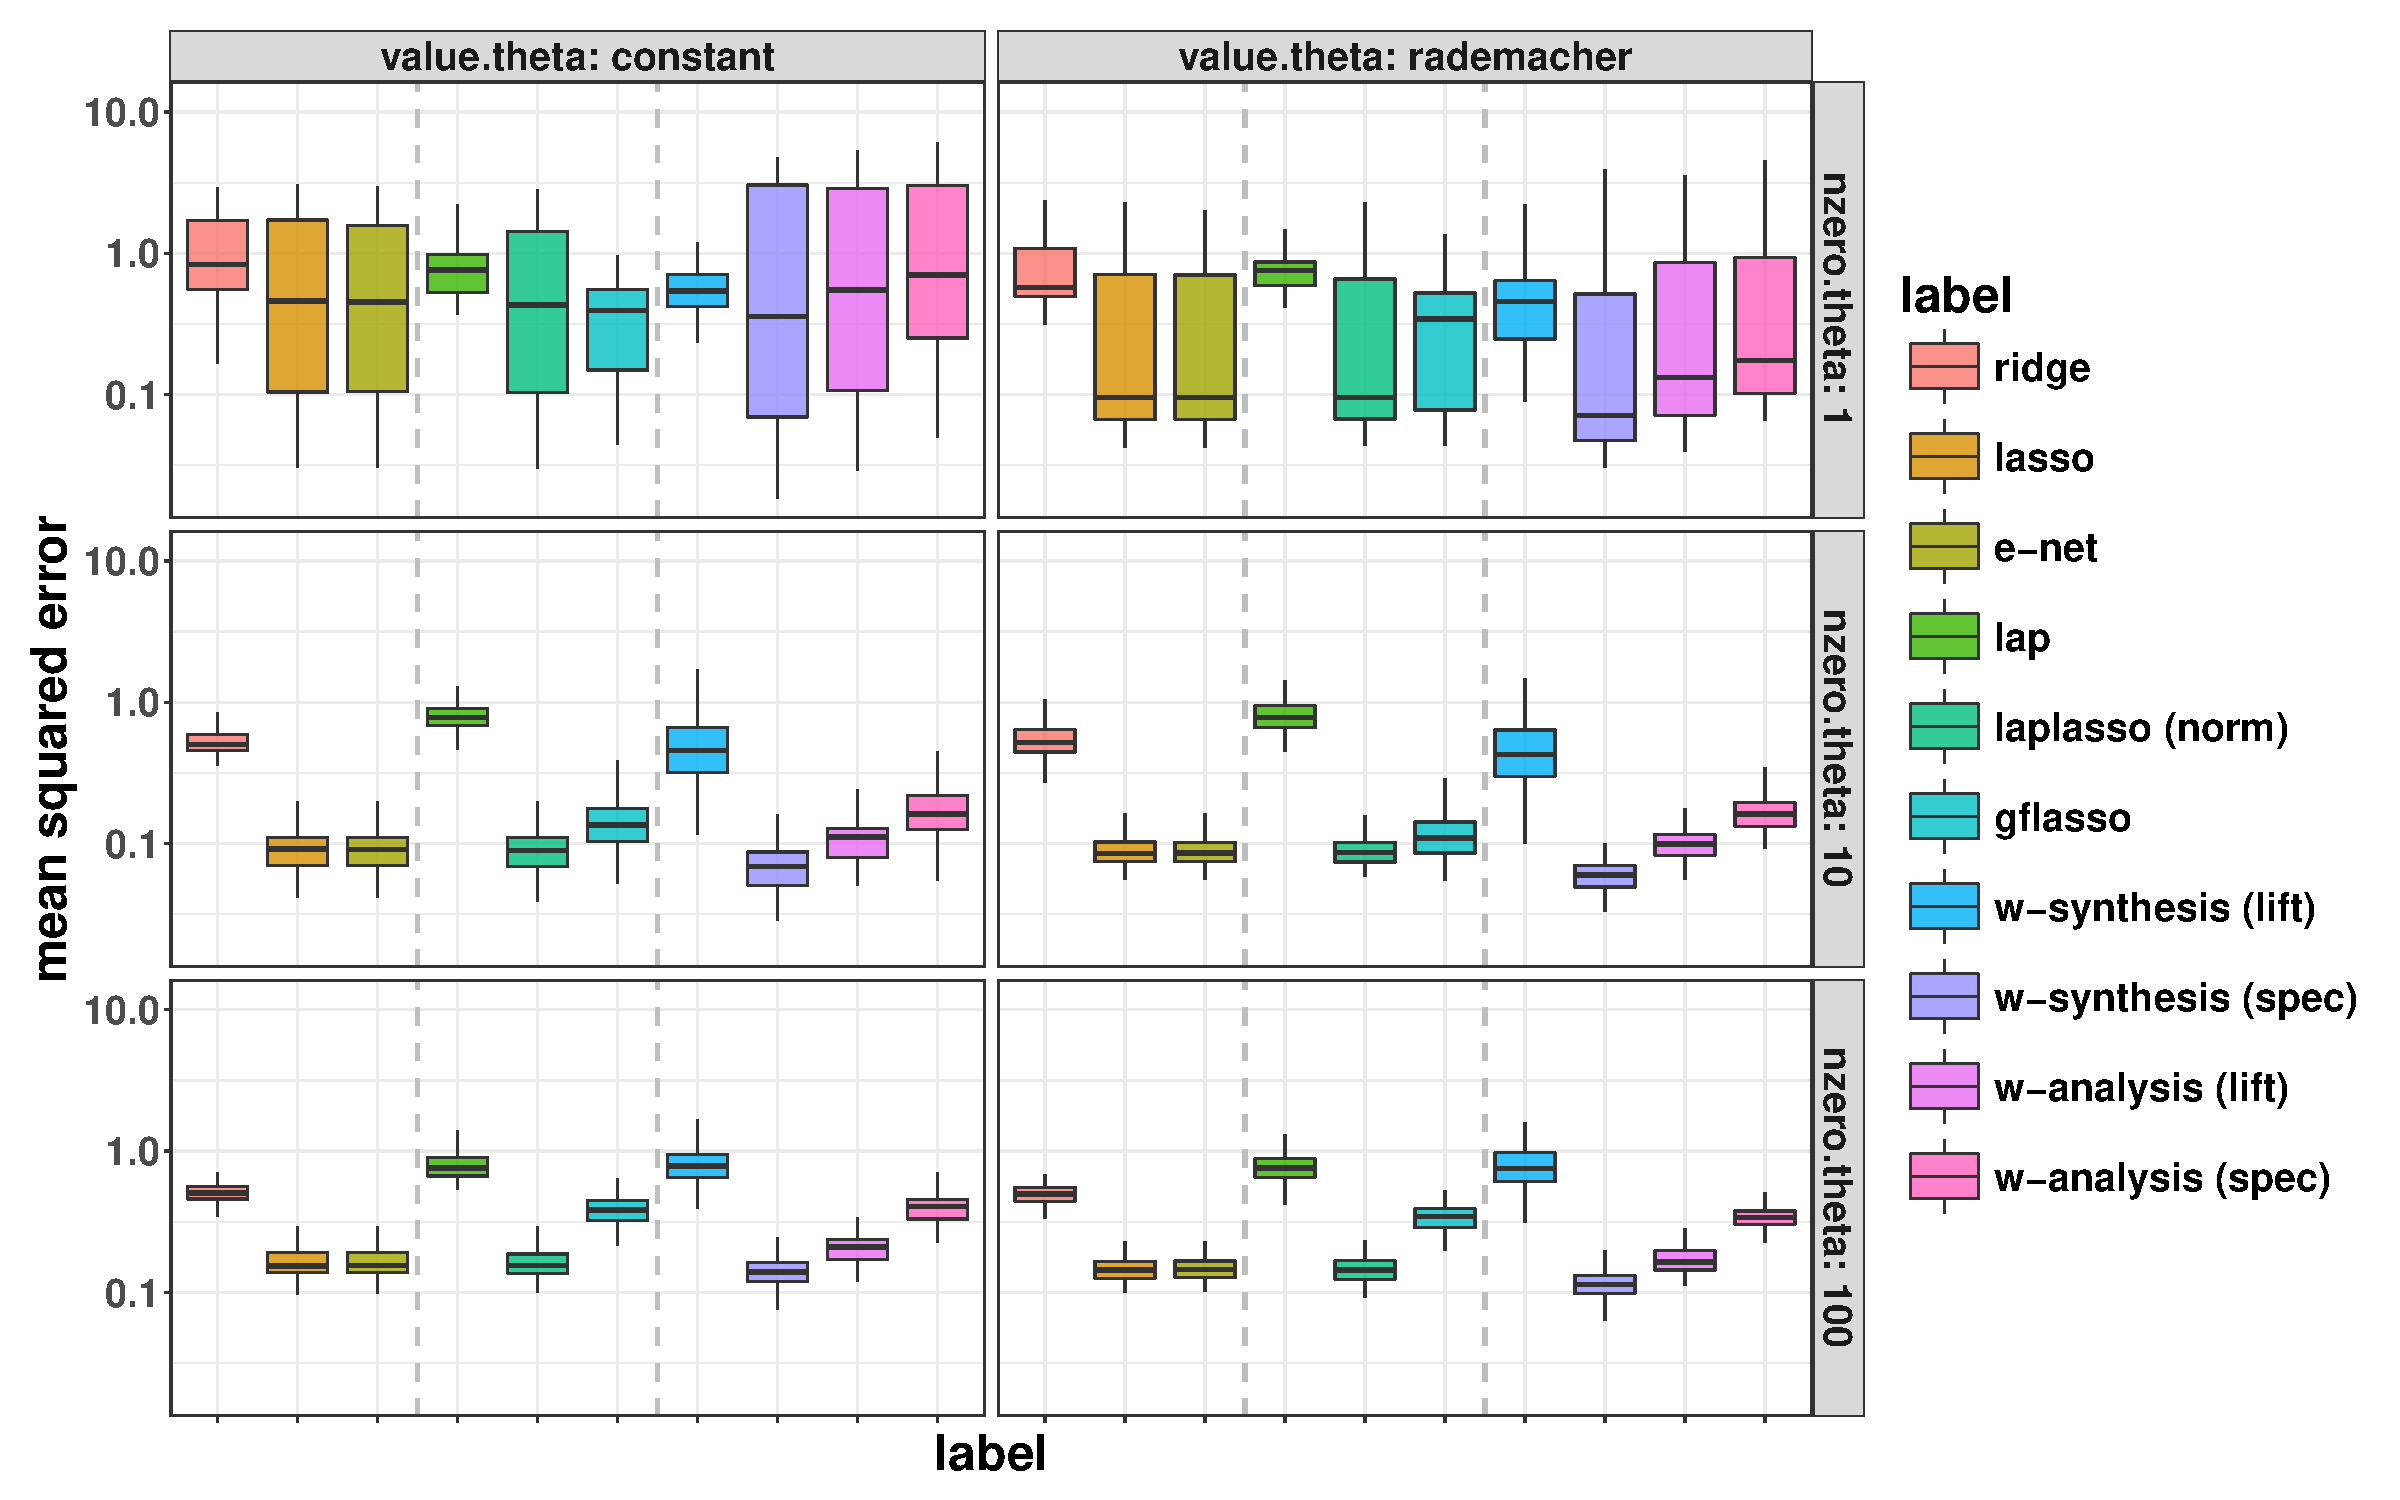
\includegraphics[width=0.9\textwidth]{ch-wavelet/plot-simulation}
	\caption{Boxplots on regression performance evaluated by prediction mean squared error over the $100$ training and test splits of the simulated data.}
	\label{fig3:simulation}
\end{figure}



On each simulated dataset, we performed $5$-fold cross-validation and evaluated the prediction mean squared error (PMSE) on each test fold, while the regularization parameters ($\lambda$ and $\nu$) were determined by nested cross-validation on each training fold. Results are shown in Figure \ref{fig3:simulation} where, under each combination of simulation set-up, boxplots present the PMSE over the $20 \times 5 = 100$ training and test splits of simulated data for a total of $10$ regularization methods including related variants. For all simulation set-ups, the wavelet-synthesis method with spectral graph wavelets denoted by ``\wsynspec{}'' is the consistent winner as expected, due to the fact that the simulated data are generated so that the informative features form locally connected subnetworks whose shapes and sizes are coherent with the spectral graph wavelets by design. The superiority is most striking when $\theta$ takes a reasonably intermediate number of non-zero coordinates, denoted by ``nzero.theta: 10'', and values that oscillate in sign, denoted by ``value.theta: rademacher''. Further, we observed that the same method with lifting-based graph wavelets instead of spectral graph wavelets, denoted by ``w-synthesis (lift)'', surprisingly exhibits the worst performance overall among all wavelet-based methods, which suggests that different approaches for constructing graph wavelets result in distinct characteristics and behaviors of underlying wavelets. However, the wavelet-analysis method is better suited with lifting-based graph wavelets than with spectral graph wavelets under our simulation set-ups, for which reasons remain unclear. Despite that the lasso and the elastic net are network-free methods, they still give competitive performance compared to the network-based Laplacian lasso or even outperform the network-based graph fused lasso in general in terms of PMSE. The two methods that do not allow for feature selection, namely the ridge and the Laplacian regularization, yield the worst prediction performance, due to the fact that the simulated data are generated by a sparse model involving only a few informative features.



\begin{figure}[!htbp]
	\centering
	\begin{subfigure}{0.9\textwidth}
		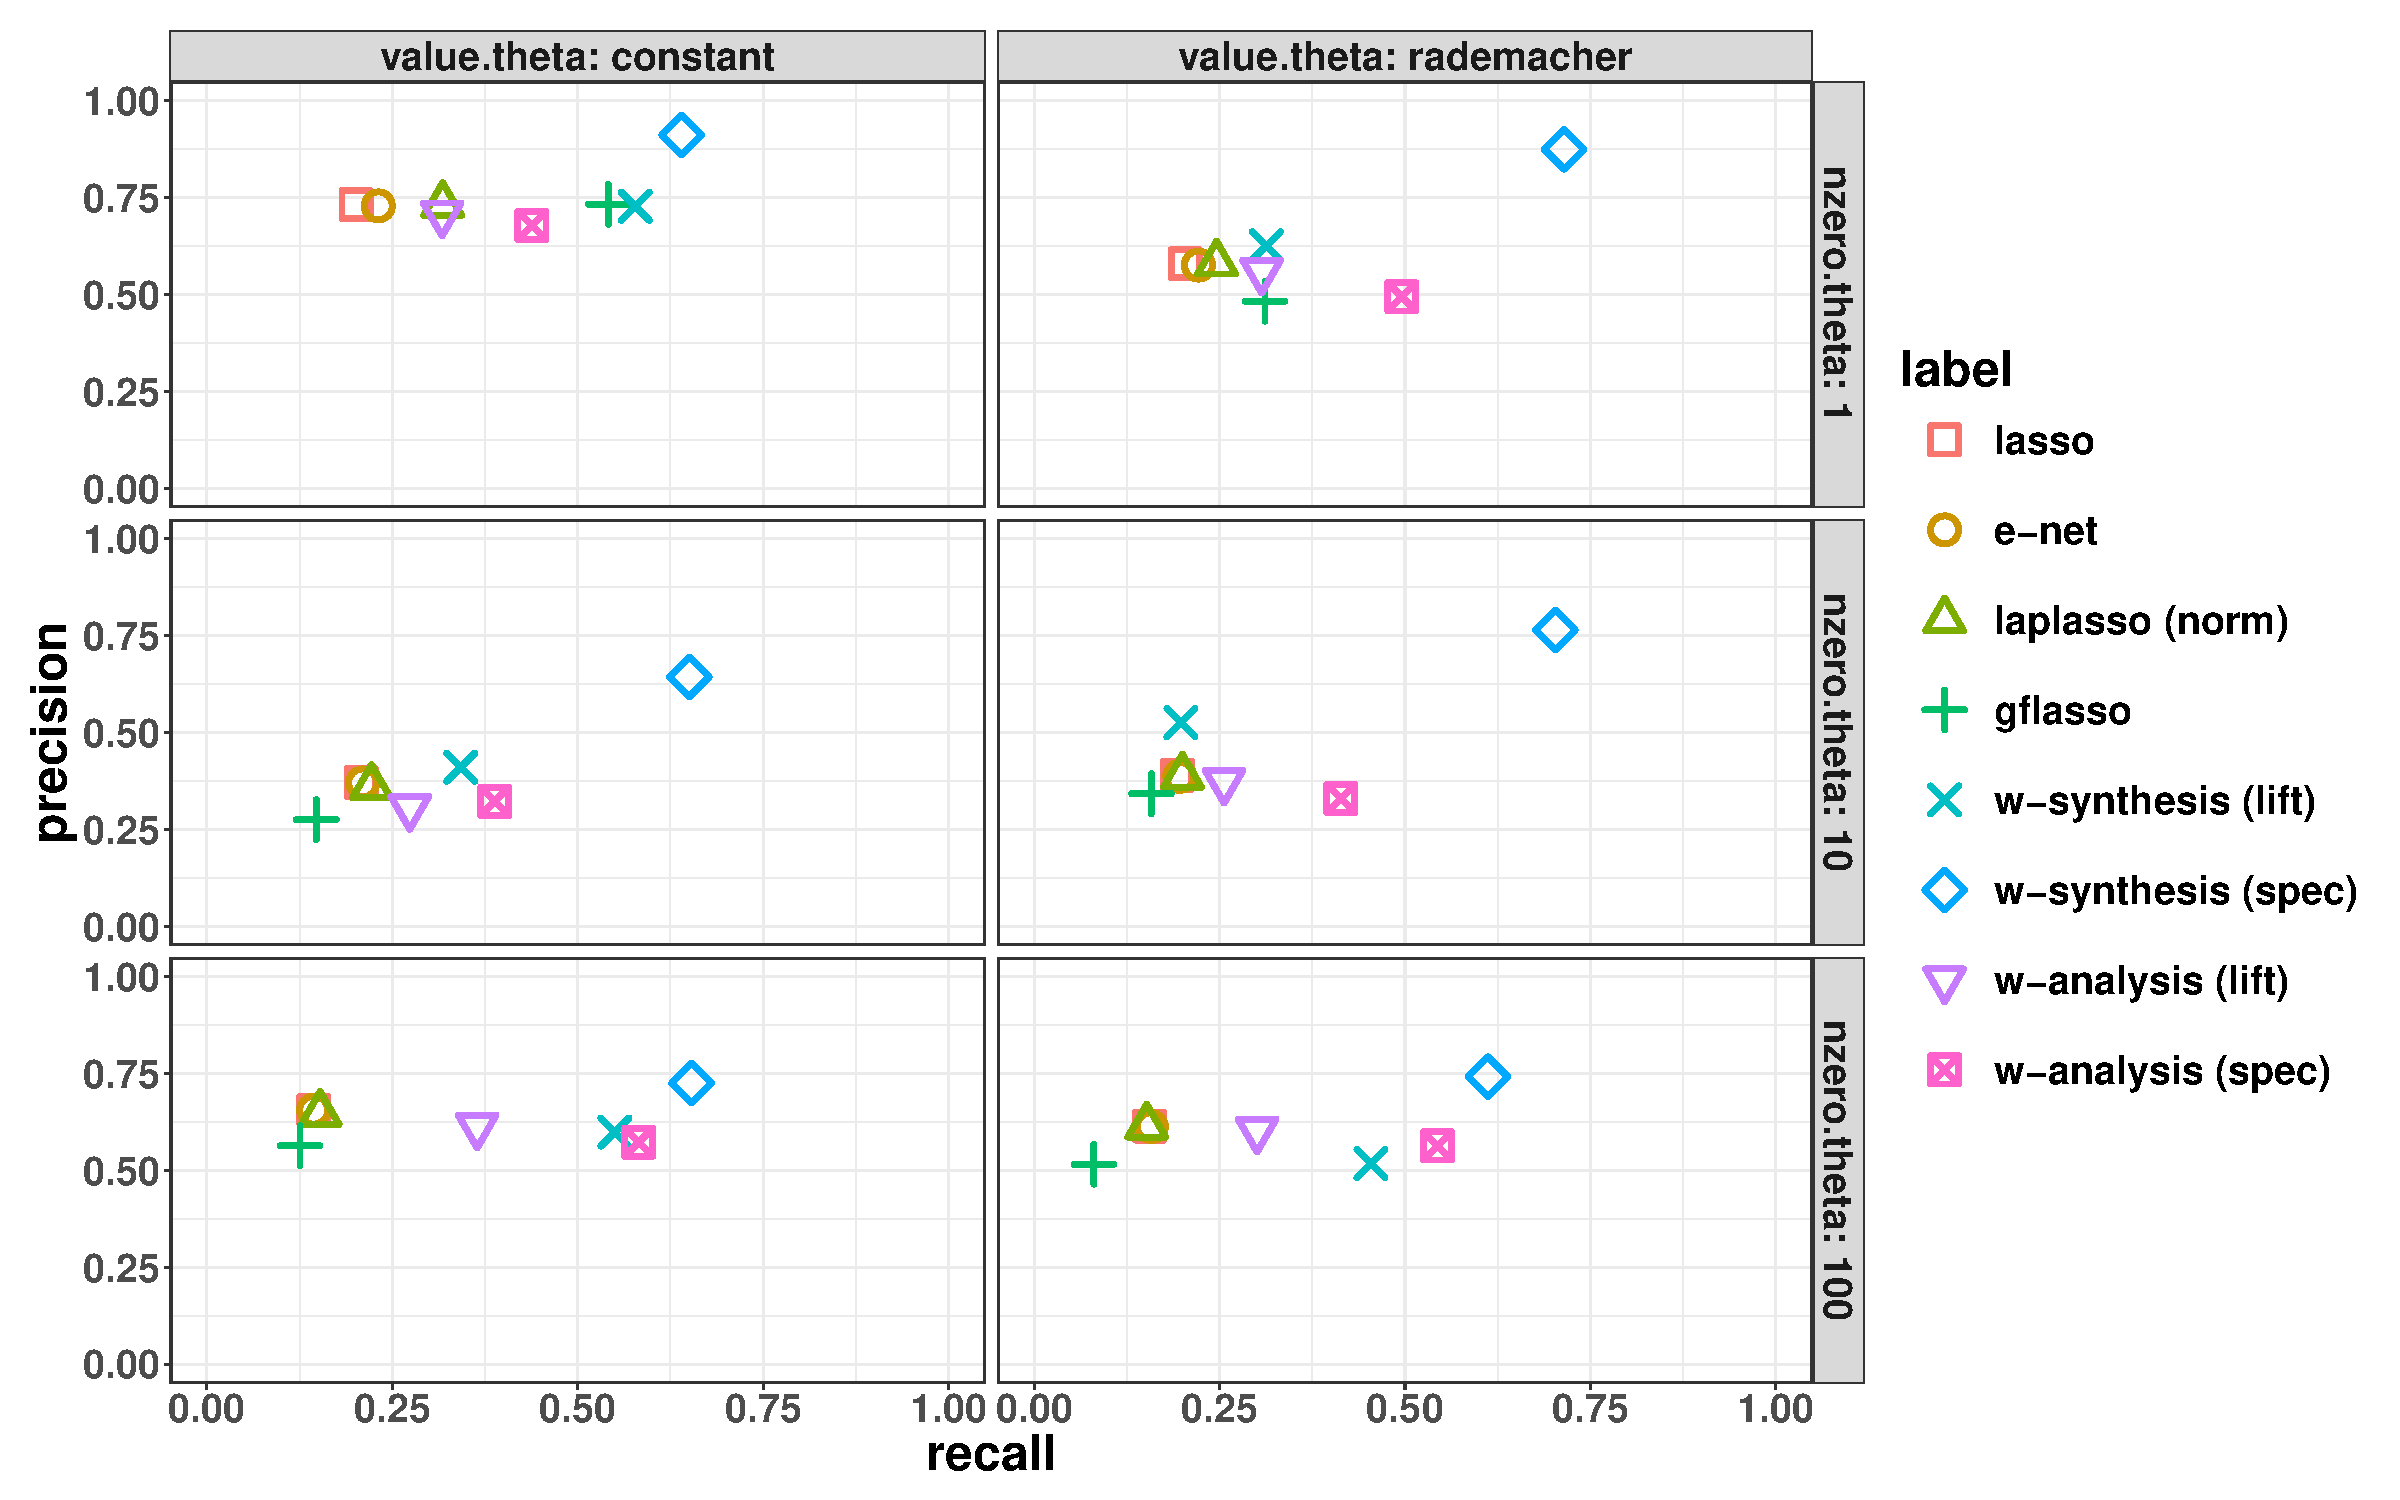
\includegraphics[width=\textwidth]{ch-wavelet/plot-support-beta}
		\caption{Support recovery of the coefficient vector $\beta$.}
		\label{fig3:support-beta}
	\end{subfigure}
	
	\begin{subfigure}{0.9\textwidth}
		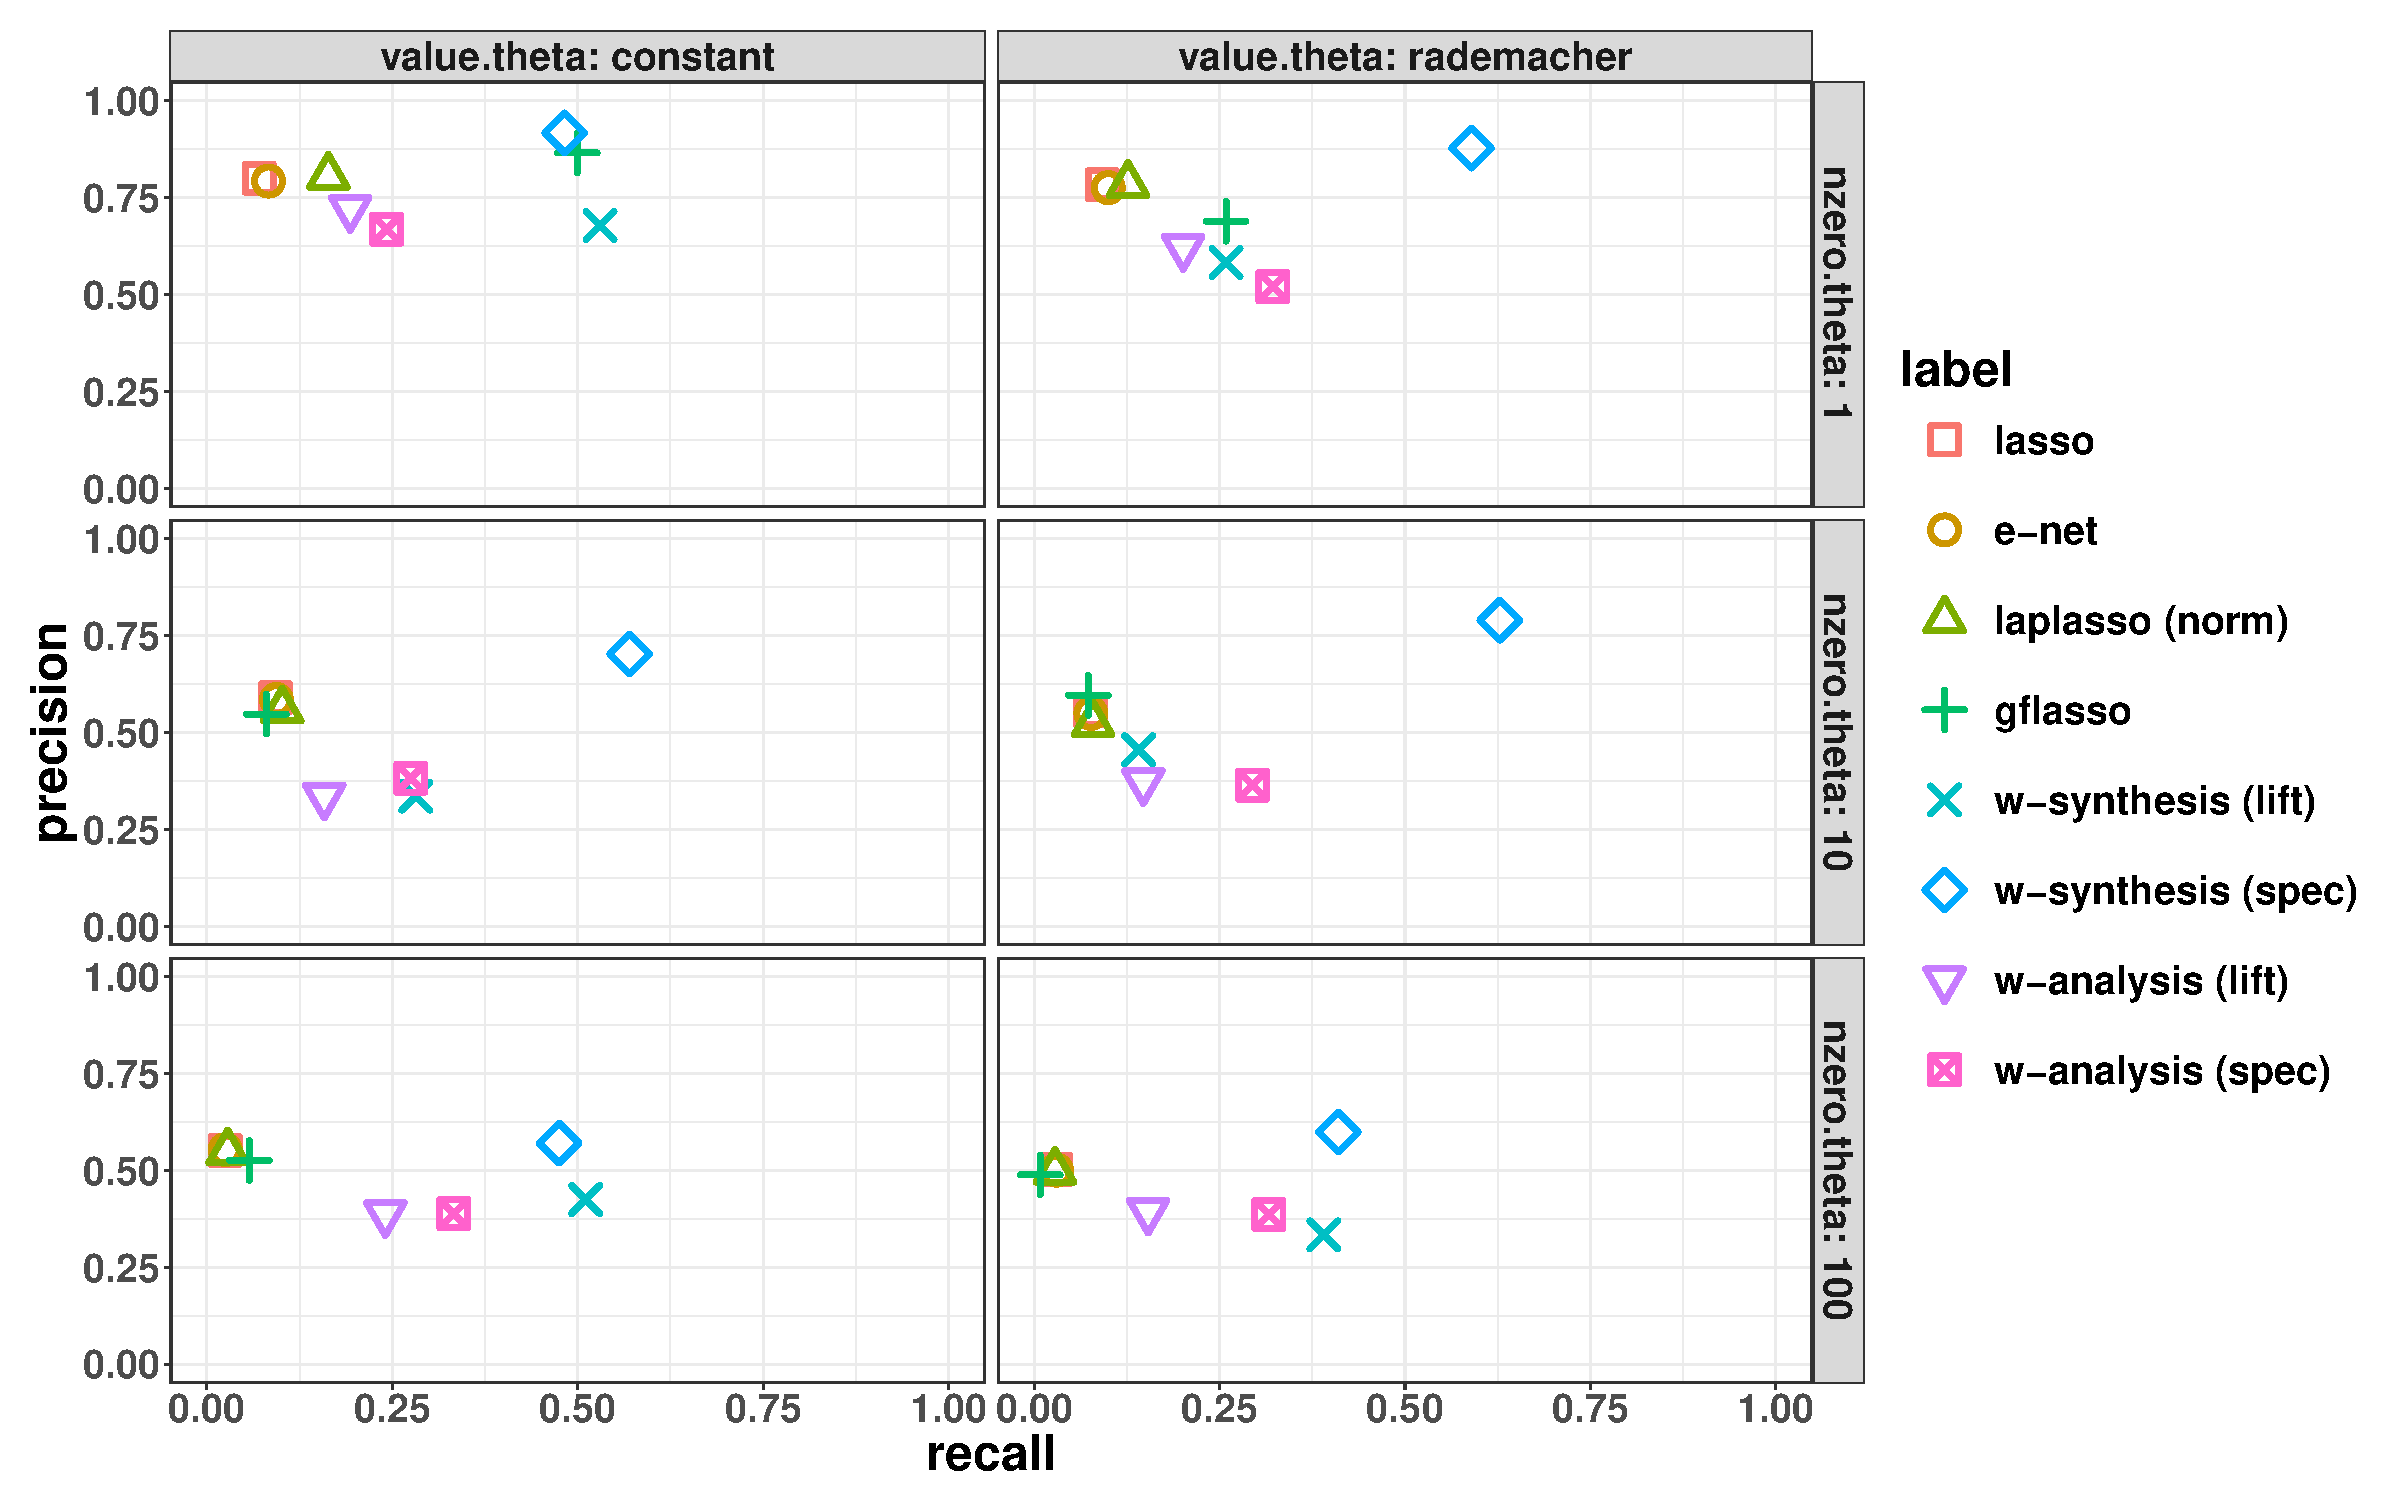
\includegraphics[width=\textwidth]{ch-wavelet/plot-support-edge}
		\caption{Support recovery of the connecting edges over the network.}
		\label{fig3:support-edge}
	\end{subfigure}
	\caption{Precision-recall plots on the recovery of simulated support of the coefficient vector $\beta$ and the connecting edges over the network.}
	\label{fig3:support}
\end{figure}


We further studied the sparsity-inducing methods which allow for feature selection regarding their ability to recover the informative features as well as the connecting edges over the network. Specifically, under a specific combination of simulation set-up, we applied each regularization method to each simulated dataset and obtained an estimate of $\beta$. We then compared the support as well as the connecting edges over the network underlying the estimated and true $\beta$ in terms of precision (the fraction of selected features that are truly informative) and recall (the fraction of truly informative features that are selected). In fact, as most values in $\beta$ are very small but not exactly zero in some cases, the ``non-zero'' support of $\beta$ is defined as the coordinates whose values are greater than one-hundredth of the largest value in $\beta$. For ease of visualization, we fit an ellipse over all the precision-recall points over the total of $20$ simulated datasets for each method, and the ellipse centers are shown in Figure \ref{fig3:support} for a total of $8$ methods including related variants. Again, the method denoted by ``\wsynspec{}'' is predominant as expected in terms of support recovery, most remarkably when $\theta$ takes a reasonably intermediate number of non-zero coordinates, denoted by ``nzero.theta: 10'', resulting in a modest number of connected subnetworks formed by the support of $\beta$. Compared to other methods, the wavelet-based methods generally tend to achieve competitive precision but much higher recall for the recovery of $\beta$ and the connecting edges over the network. Surprisingly, when the number of informative features becomes large and hence more connected over the network, the network-based Laplacian lasso and graph fused lasso does not distinguishingly outperform the network-free lasso and elastic net in terms of feature selection or even edge identification.



\subsection{Breast Cancer Survival Analysis}
\label{sec3:breastcancer}


For \textit{in vivo} experiments, we performed survival analysis for breast cancer using the METABRIC data guided by the HPRD PPI network. In fact, for each breast tumor sample, the METABRIC dataset additionally provides clinical information on the overall survival time of the underlying patient, that is either the exact number of days dating from initial consultation until the patient passed away or the number of days until the patient is last seen alive. This clinical information was converted to right-censored survival data and we performed survival risk prediction for breast cancer.


\begin{figure}[!htbp]
\centering
	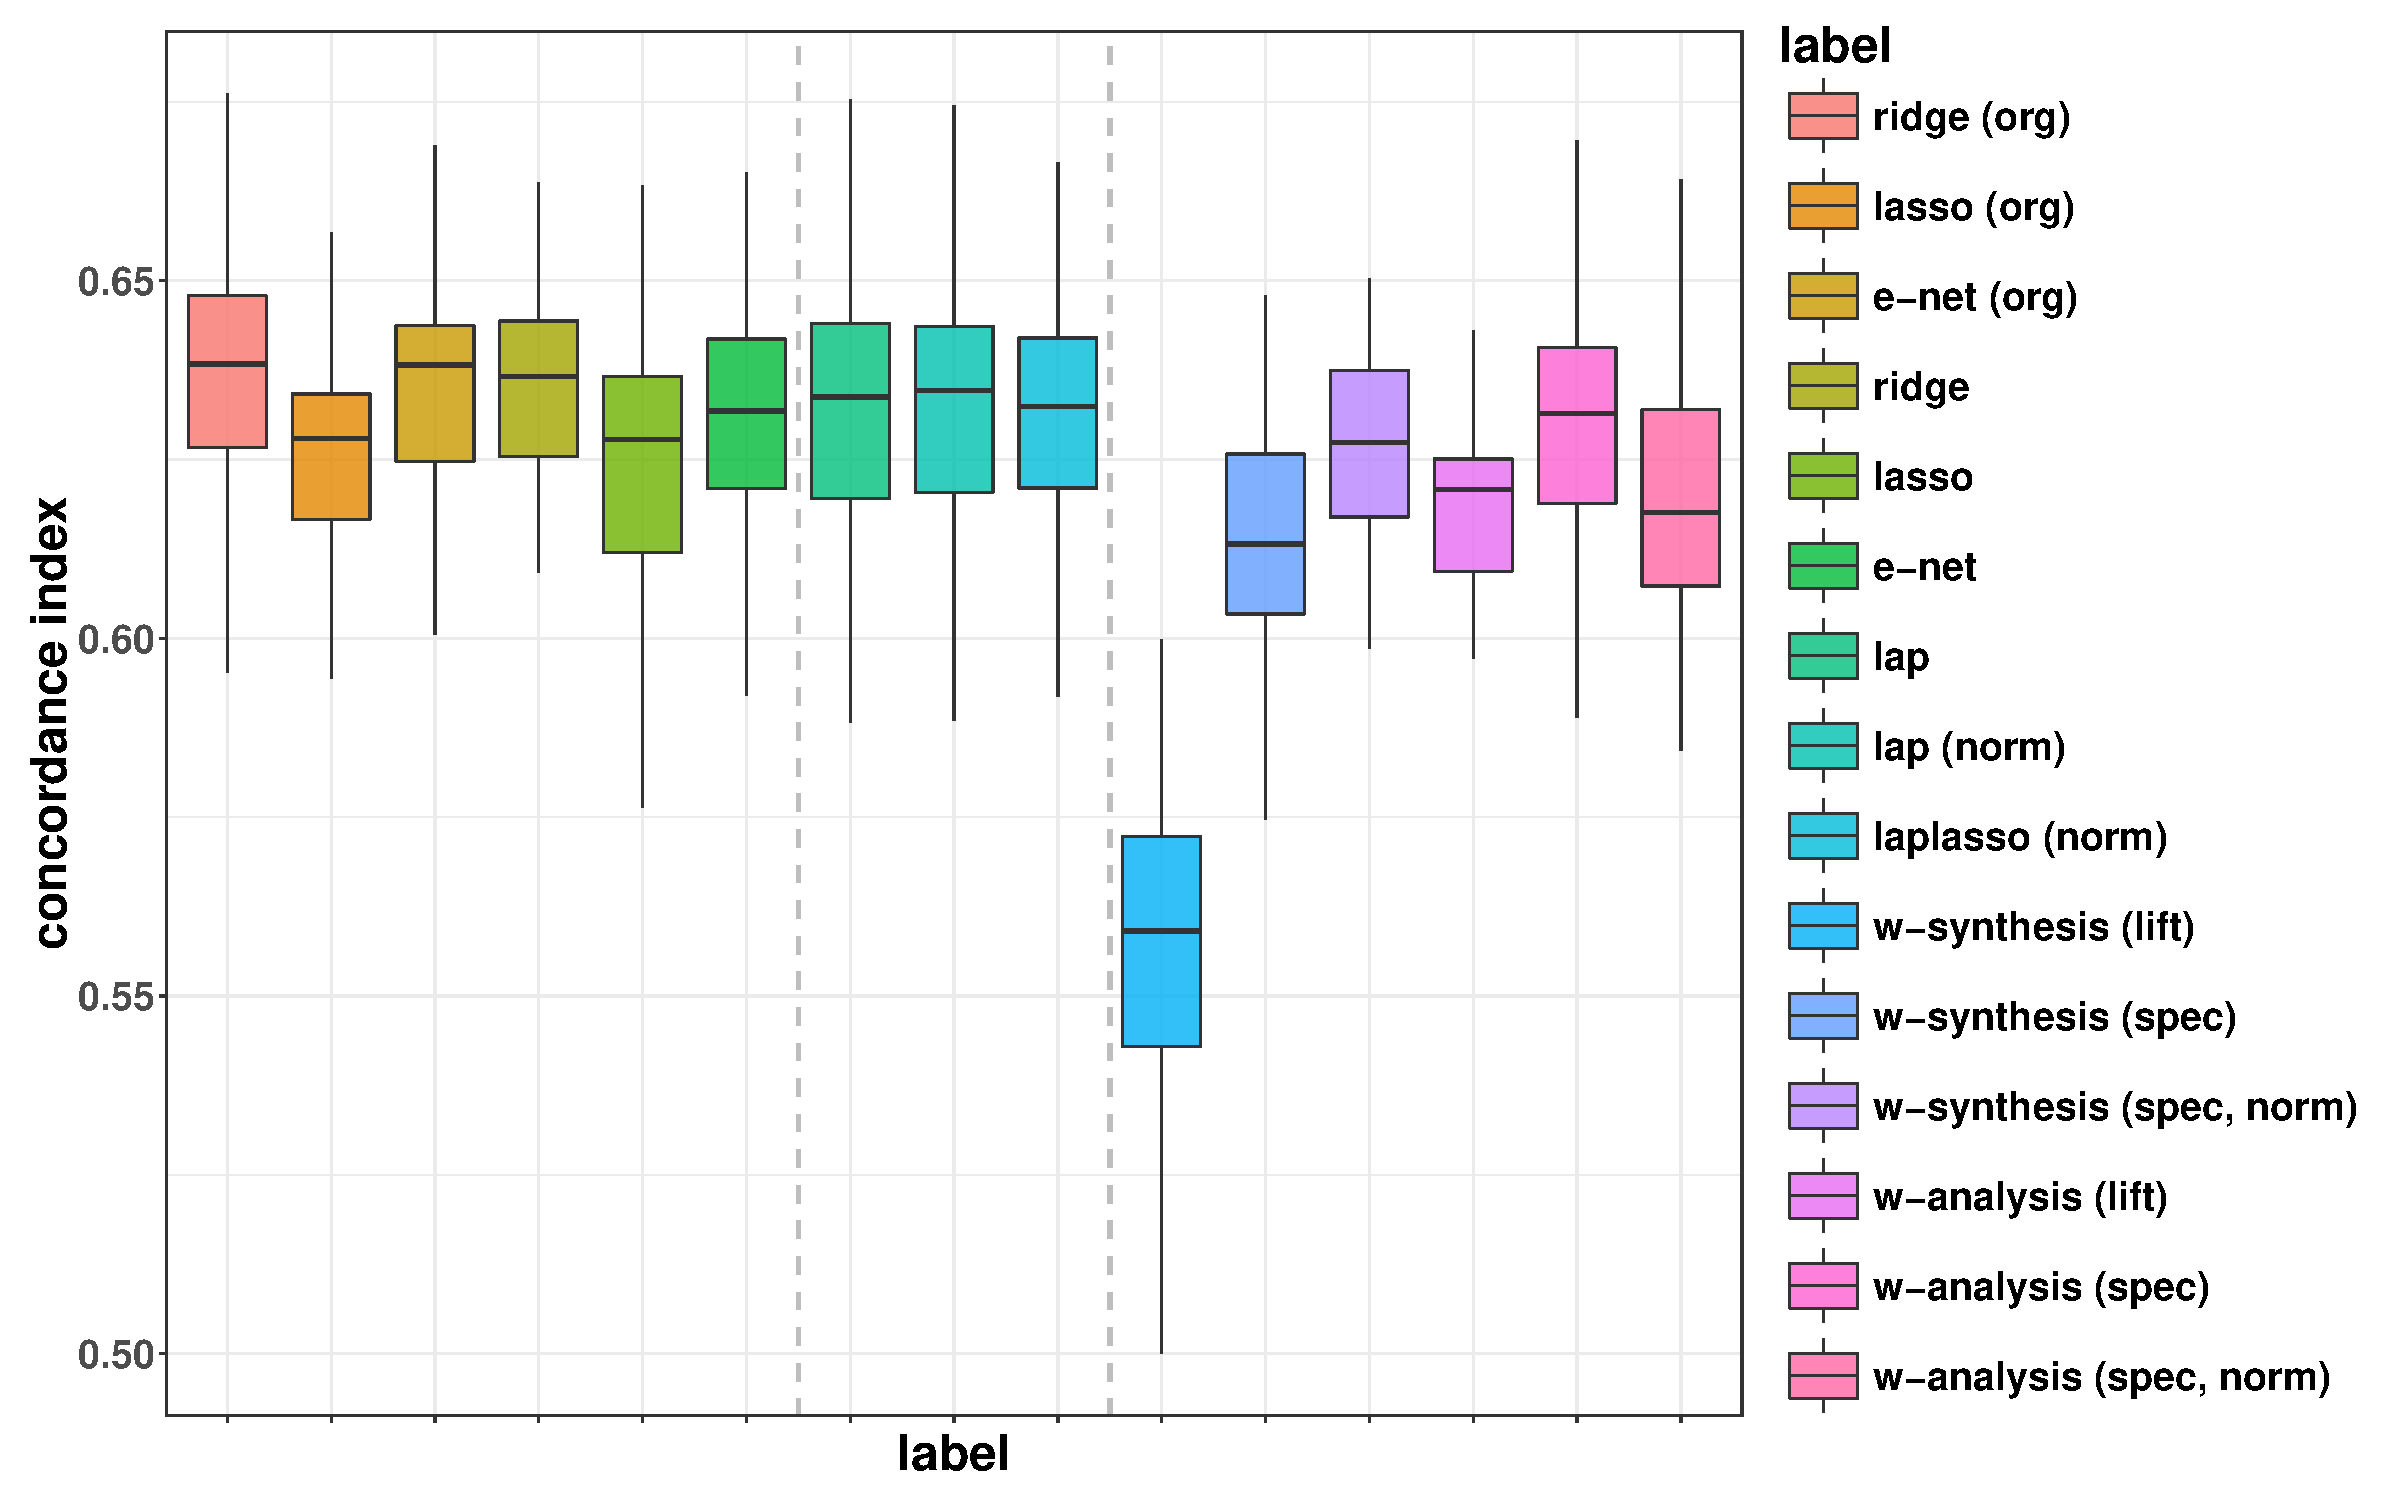
\includegraphics[width=0.9\textwidth]{ch-wavelet/plot-prediction}
	\caption{Boxplots on survival risk prediction performance evaluated by concordance index scores over 5-fold cross-validation repeated 10 times of the METABRIC data.}
	\label{fig3:prediction}
\end{figure}



\begin{table}[!htbp]
\centering
\caption{Mean concordance index (CI) scores ($\pm$ standard deviation) of survival risk prediction over 5-fold cross-validation repeated 10 times of the METABRIC data. Methods are ordered by decreasing mean CI scores.}
\small
	\begin{tabular}{c|c|c|c}
	\hline
	Label & Mean CI scores ($\pm$ SD) & Network-based & Feature selection \\\hline
	ridge (org)	&	$0.637 \, (\pm 0.0178$)	&	& \\
	ridge	&	$0.636 \, (\pm 0.018$)	&	& \\
	e-net (org)	&	$0.6345 \, (\pm 0.0185$)	&	& $\checkmark$ \\
	lap (norm)	&	$0.633 \, (\pm 0.0196$)	& $\checkmark$	& \\
	lap	&	$0.632 \, (\pm 0.0193$)	& $\checkmark$	& \\
	laplasso (norm)	&	$0.6312 \, (\pm 0.0185$)	& $\checkmark$	& $\checkmark$ \\
	e-net	&	$0.6304 \, (\pm 0.0183$)	&	& $\checkmark$ \\
	\wanaspec	&	$0.6295 \, (\pm 0.0198)$	& $\checkmark$	& $\checkmark$ \\
	\wsynspecnorm	&	$0.6264 \, (\pm 0.018)$	& $\checkmark$	& $\checkmark$ \\
	lasso	&	$0.626 \, (\pm 0.0177)$	&	& $\checkmark$ \\
	lasso (org)	&	$0.6257 \, (\pm 0.0172)$	&	& $\checkmark$ \\
	\wanaspecnorm	&	$0.6216 \, (\pm 0.0228)$	& $\checkmark$	& $\checkmark$ \\
	w-analysis (lift)	&	$0.6163 \, (\pm 0.0182)$	& $\checkmark$	& $\checkmark$ \\
	\wsynspec	&	$0.6157 \, (\pm 0.0184)$	& $\checkmark$	& $\checkmark$ \\
	w-synthesis (lift)	&	$0.5587 \, (\pm 0.0232)$	& $\checkmark$	& $\checkmark$ \\
	\hline
	\end{tabular}
\label{tab3:prediction}
\end{table}




The first objective of the \textit{in vivo} investigation is to compare the survival risk prediction performance of different regularization methods. To this end, we performed $5$-fold cross-validation repeated $10$ times on the full METABRIC dataset and evaluated the concordance index (CI) scores on each test fold, while the regularization parameters ($\lambda$ and $\nu$) were determined by nested cross-validation on each training fold. Note that CI is a measure of rank-based consistency between the predicted survival risk and observed survival time for a cohort of patients, in the sense that it is an estimate of the probability that, given two randomly drawn patients, the patient who survives longer is predicted with a lower risk. Results are shown in Figure \ref{fig3:prediction} with boxplots over the $10 \times 5 = 50$ splits of training and test data and in Table \ref{tab3:prediction} with mean CI scores ($\pm$ standard deviation) for a total of $15$ regularization methods including related variants. The ridge is the best-performing model in terms of mean CI scores but it does not allow for feature selection, and among methods that enable feature selection, the elastic net is the best-performing one. Notably, both methods are regardless of the prior knowledge encoded in the network. Among network-based methods that enable feature selection, the best-performing one is the Laplacian lasso, followed by the wavelet-analysis method with spectral graph dual wavelets. We observed that the wavelet-based methods provide relatively less accurate survival risk prediction in terms of CI scores compared to other methods. We performed two-sided t-tests to statistically quantify the difference of the cross-validation CI scores between each pair of methods. FDR-adjusted p-values suggest that, at the significance level $0.05$, there is no significant decrease in the prediction performance for the best-performing wavelet-based method, namely the method denoted by ``\wanaspec{}'', compared to any of the methods tested. Notably, network-free methods using the entire list of genes available from the METABRIC data does not significantly improve the survival risk prediction performance, compared to those using the subset of genes only found on the HPRD PPI network. This justifies that the loss is not significant when our analysis is restrained to the subset of genes found on the network. For detailed results regarding the statistical tests, we refer to the online supplements. Another interesting observation regarding wavelet-based methods is that, as the spectral graph wavelets are constructed using graph Laplacian that appear in either normalized or non-normalized version, the wavelet-analysis method is better suited with the non-normalized version while the wavelet-synthesis method is better suited with the normalized version, for which reasons remain unclear.



The focus of \textit{in vivo} experiments in this study is to select genes that are related to breast cancer survival, and in particular we favor methods that result in a list of selected genes that tend to form gene modules on the HPRD PPI network potentially by making use of their biological interaction known \textit{a priori}. To this end, we then compared the goodness of gene selection of different methods from several aspects, namely stability, connectivity and interpretability. Note that only those $9$ methods including related variants that enable feature selection are discussed for the remainder of this section.



\begin{figure}[!htbp]
\centering
	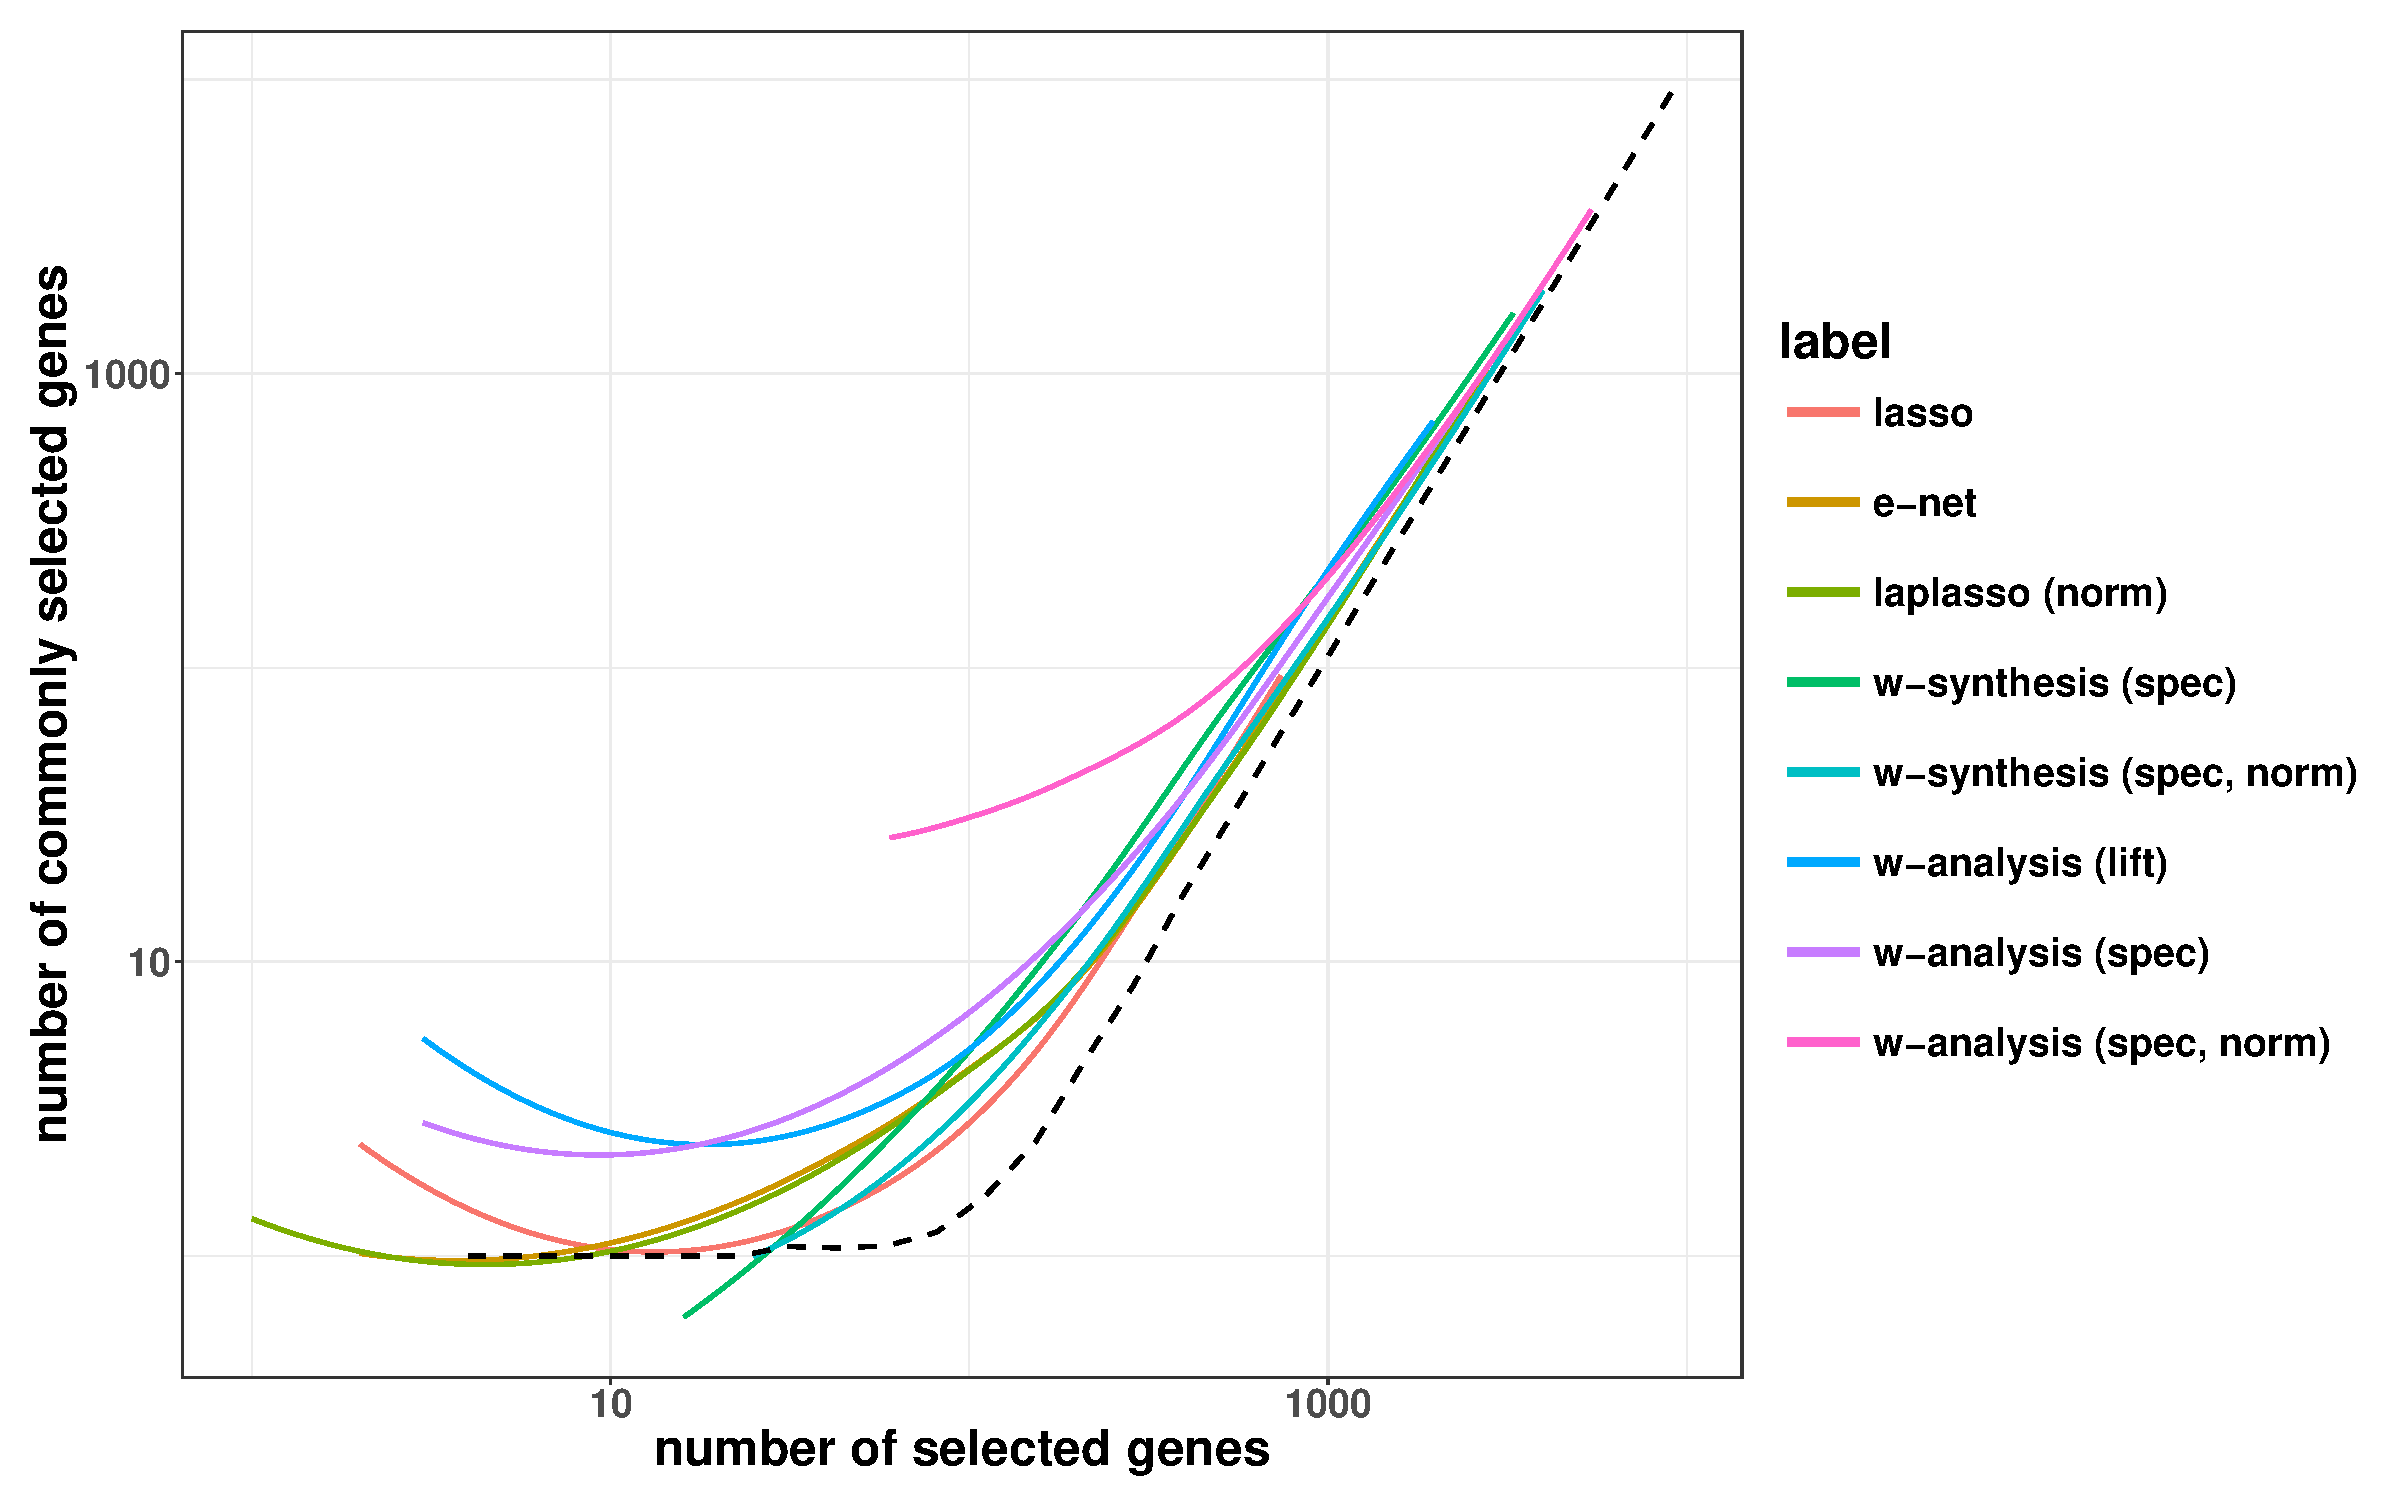
\includegraphics[width=0.9\textwidth]{ch-wavelet/plot-stability}
	\caption{Stability performance of gene selection related to breast cancer survival, estimated over $100$ random experiments. The black dotted curve denotes random selection.}
	\label{fig3:stability}
\end{figure}



Stability is an important concept that advocates reproducibility of selecting the significant features across independent studies. In order to compare stability of feature selection by different methods, we randomly split the full METABRIC dataset evenly into two halves and obtained a pair of models independently trained on the two disjoint subsets with the same method. Then constraining on each fixed number of genes selected, we computed the number of commonly selected genes between the two independent models as a score indicating stability. We repeatedly split the data $100$ times to address the randomness in splitting the data. For ease of visualization, we applied locally weighted scatterplot smoothing (LOESS) \cite{Cleveland1979Robust} to all the stability scores for each method and thus obtained a curve of stability scores along the solution path. Results are shown in Figure \ref{fig3:stability}. We observed that the number of commonly selected genes between pairs of independent models tends to become larger as the number of selected genes increases. As we are most interested in selecting typically a few hundreds of genes that could interestingly form subnetworks of modest sizes, the wavelet-based method denoted by ``\wanaspecnorm{}'' distinguishingly won in terms of stability at the scale of $10^2$ genes selected, followed by two other wavelet-based methods denoted by ``\wanaspec{}'' and ``\wsynspec{}''. Recall that the method denoted by ``\wanaspec{}'' is the best-performing method in terms of CI scores for survival risk prediction. Last but not least, the network-free methods, namely the lasso and elastic net, and network-based Laplacian lasso provide feature selection procedures that are overall less stable. Further, as negative-control experiment, we randomly selected twice the same number of genes along the solution path and counted the number of commonly selected genes. At each fixed number of genes selected, the number of commonly selected genes is averaged over $100$ repeats to address the randomness. A stability curve for random selection is shown by the black dotted curve in the figure. Note that all methods tested in this study outperform the random selection in terms of stability, especially strikingly at the scale of $10^2$ genes selected.



\begin{figure}[!htbp]
\centering
	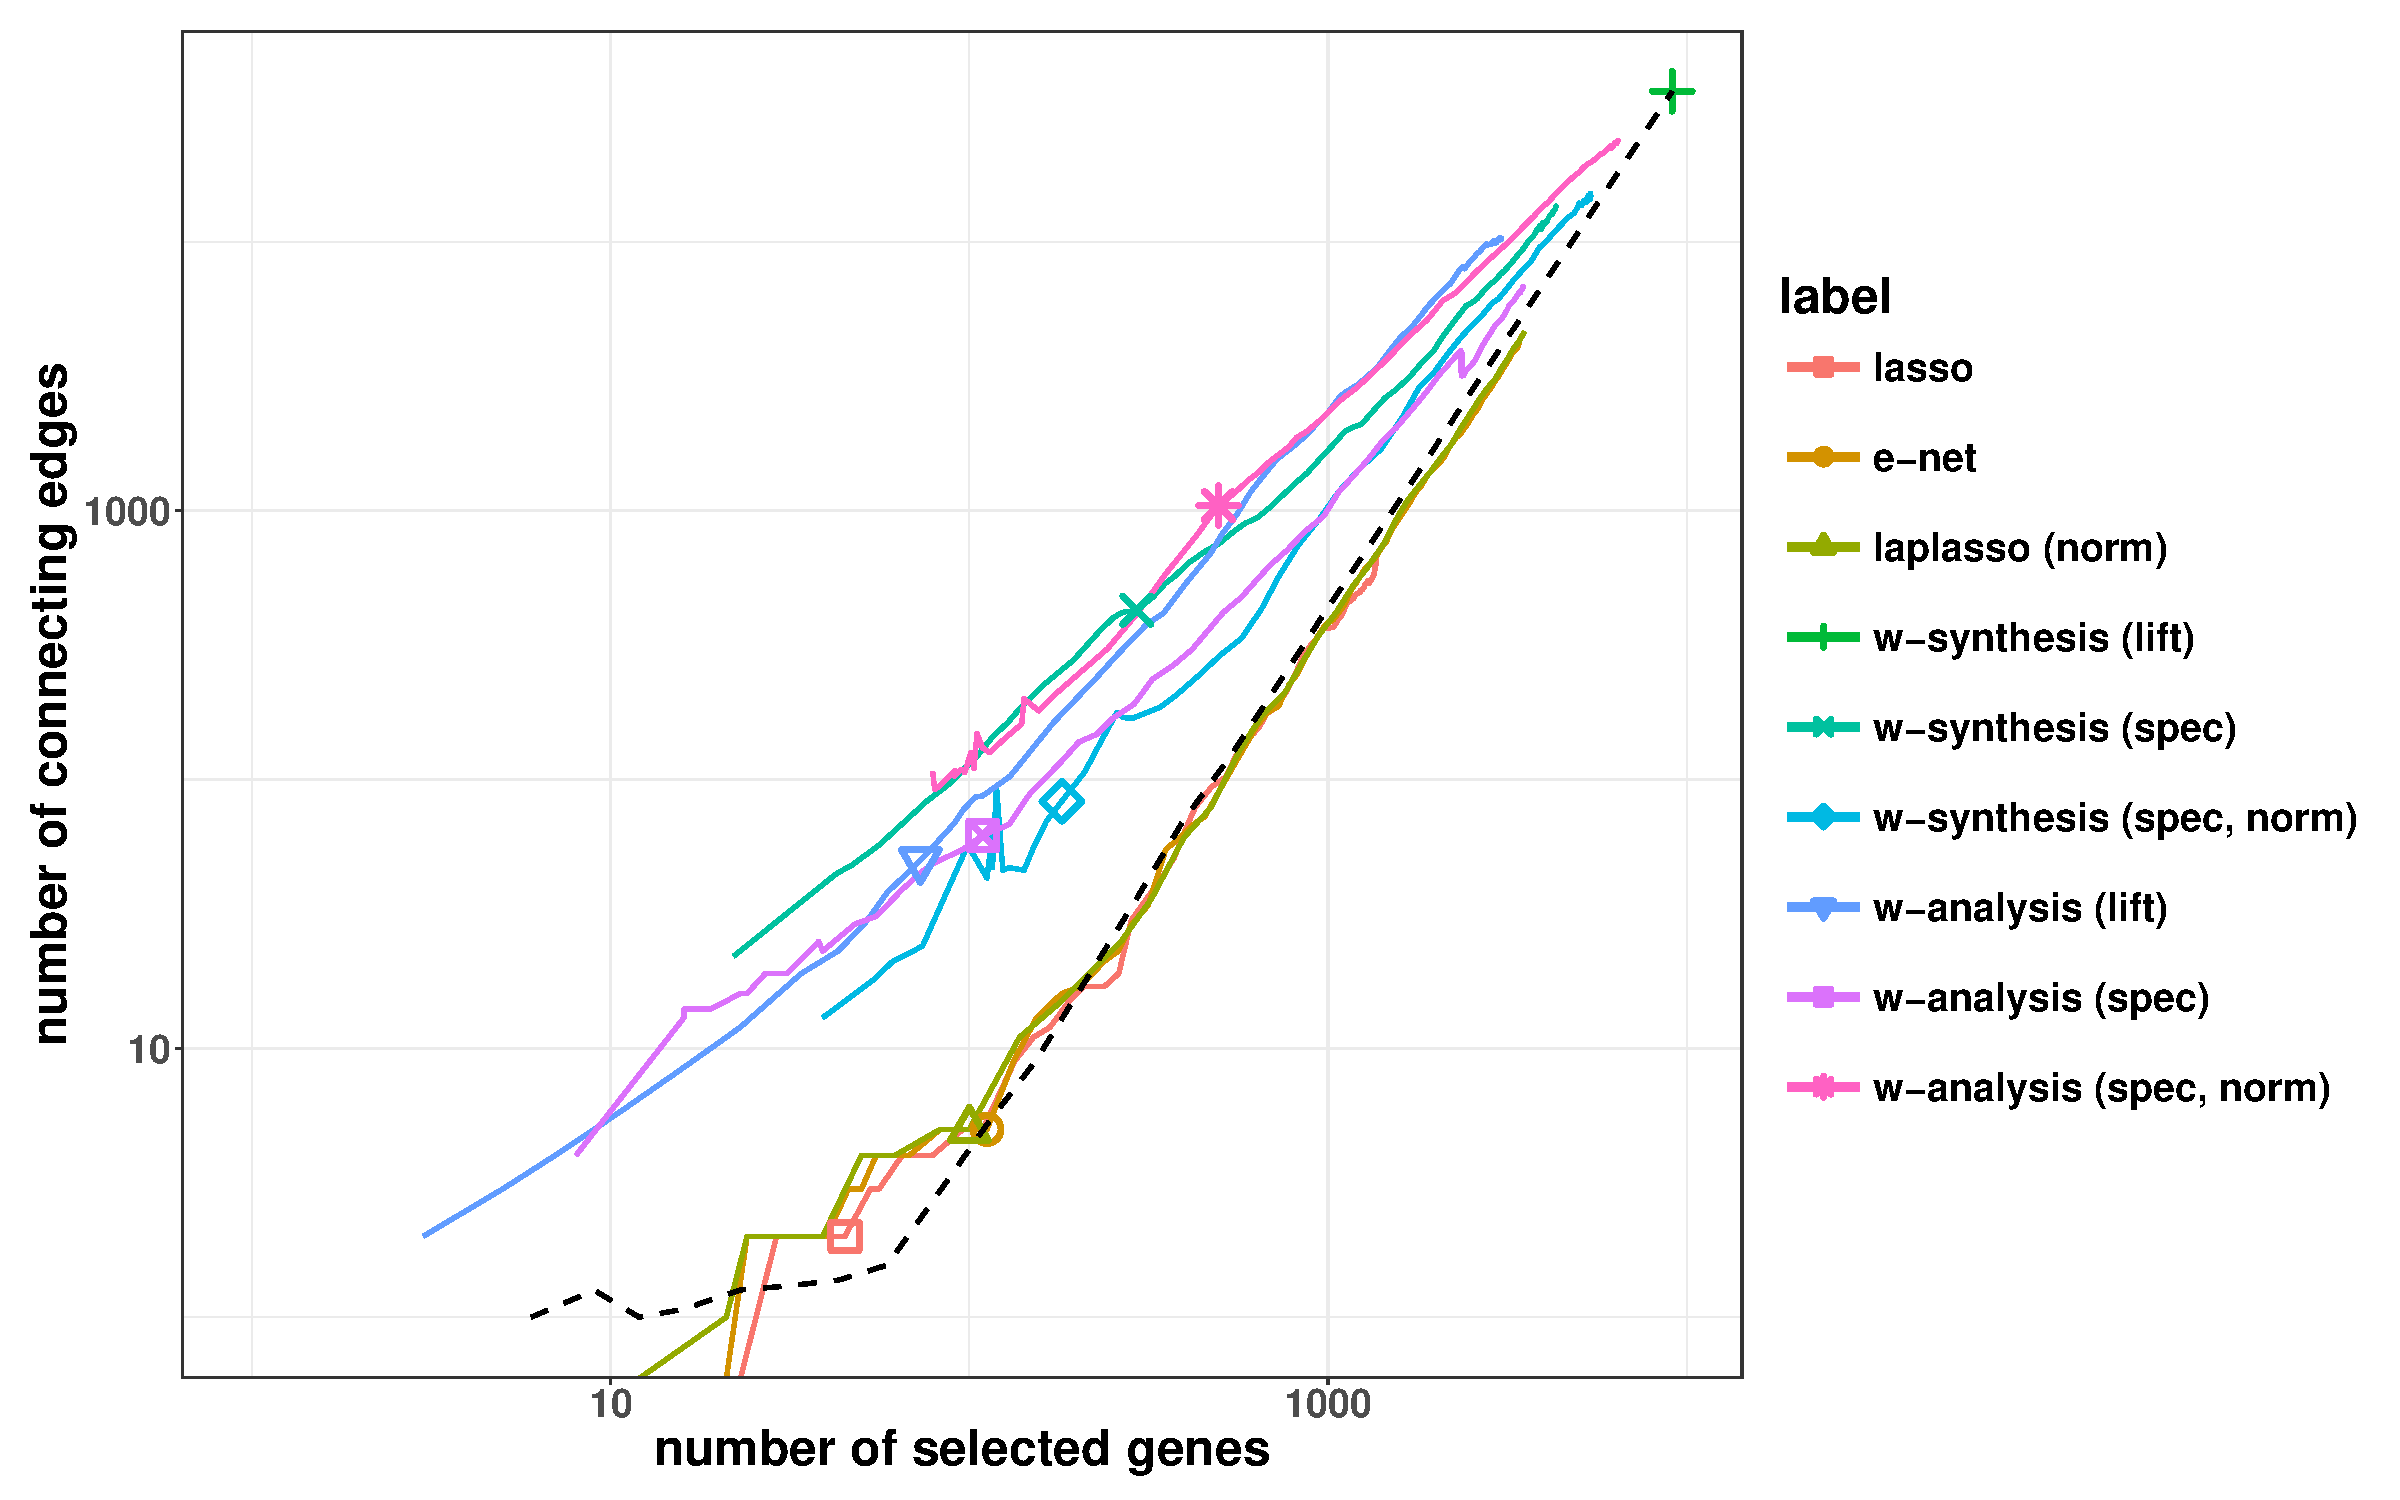
\includegraphics[width=0.9\textwidth]{ch-wavelet/plot-connectivity}
	\caption{Connectivity performance of gene selection related to breast cancer survival, where special marks correspond to the number tuned by cross-validation. The black dotted curve denotes random selection.}
	\label{fig3:connectivity}
\end{figure}



Recall from the introduction that the motivation of this study is to encourage selected features to be connected given a network, and for that purpose, we would like to quantitatively compare feature selection in terms of connectivity over the given network. A model is trained by applying each method to the full METABRIC dataset and, constraining on each fixed number of genes selected, a connectivity score is defined as the number of connecting edges between the selected genes. Thus for each method we obtained a curve of connectivity scores along the solution path. Results are shown in Figure \ref{fig3:connectivity}, where special marks indicate the number of genes and connecting edges that was determined by tuning the regularization parameter $\lambda$ by cross-validation. We observed that the wavelet-based methods remarkably outperform other methods in terms of connectivity in general. In particular, the method denoted by ``\wanaspecnorm{}'' that has stood out in terms of stability remains to be one of the top-performing methods in terms of connectivity, whereas it selected a relatively large number of genes by cross-validation. It is worth special mention that the method denoted by ``\wanaspec{}'' selected around $10^2$ genes by cross-validation that attain a reasonably good number of connecting edges, and it has been one of the top-performing methods in terms of stability in feature selection when this number of genes is selected, and it also remains competitive to all other methods in terms of CI scores for survival risk prediction. A side note on the strange performance of the method denoted by ``w-synthesis (lift)'' is that this method output an estimate of $\beta$ that is constant\footnote{Due to numerical instability in computation, there may exist infinitesimal variations in the values of estimated $\beta$ output by the method.} when fitted to the full METABRIC dataset particularly, and consequently the full list of genes were considered as selected. Further, as negative-control experiment, we randomly selected a certain number of genes regardless of a network, and counted the number of connecting edges over the given network. At each fixed number of genes selected, the number of connecting edges is averaged over $100$ repeats to address the randomness. A connectivity curve for random selection is shown by the black dotted curve in the figure. Note that the network-free methods, namely the lasso and the elastic net, and network-based Laplacian lasso do not seem to significantly outperform the random selection in terms of connectivity.



\begin{figure}[!htbp]
	\centering
	\begin{subfigure}{0.9\textwidth}
		\centering
		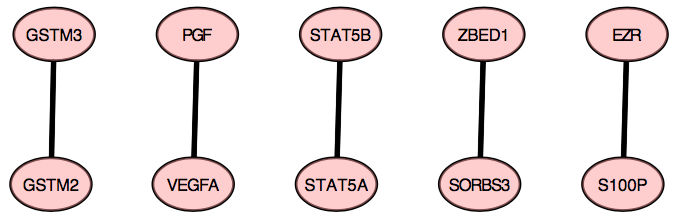
\includegraphics[width=0.5\textwidth]{ch-wavelet/subnetworks_e-net}
		\caption{Gene subnetworks identified by the elastic net ($10$ genes connected out of $112$ selected) or the Laplacian lasso ($10$ genes connected out of $100$ selected).}
		\label{fig3:enet}
	\end{subfigure}
	
	\begin{subfigure}{0.9\textwidth}
		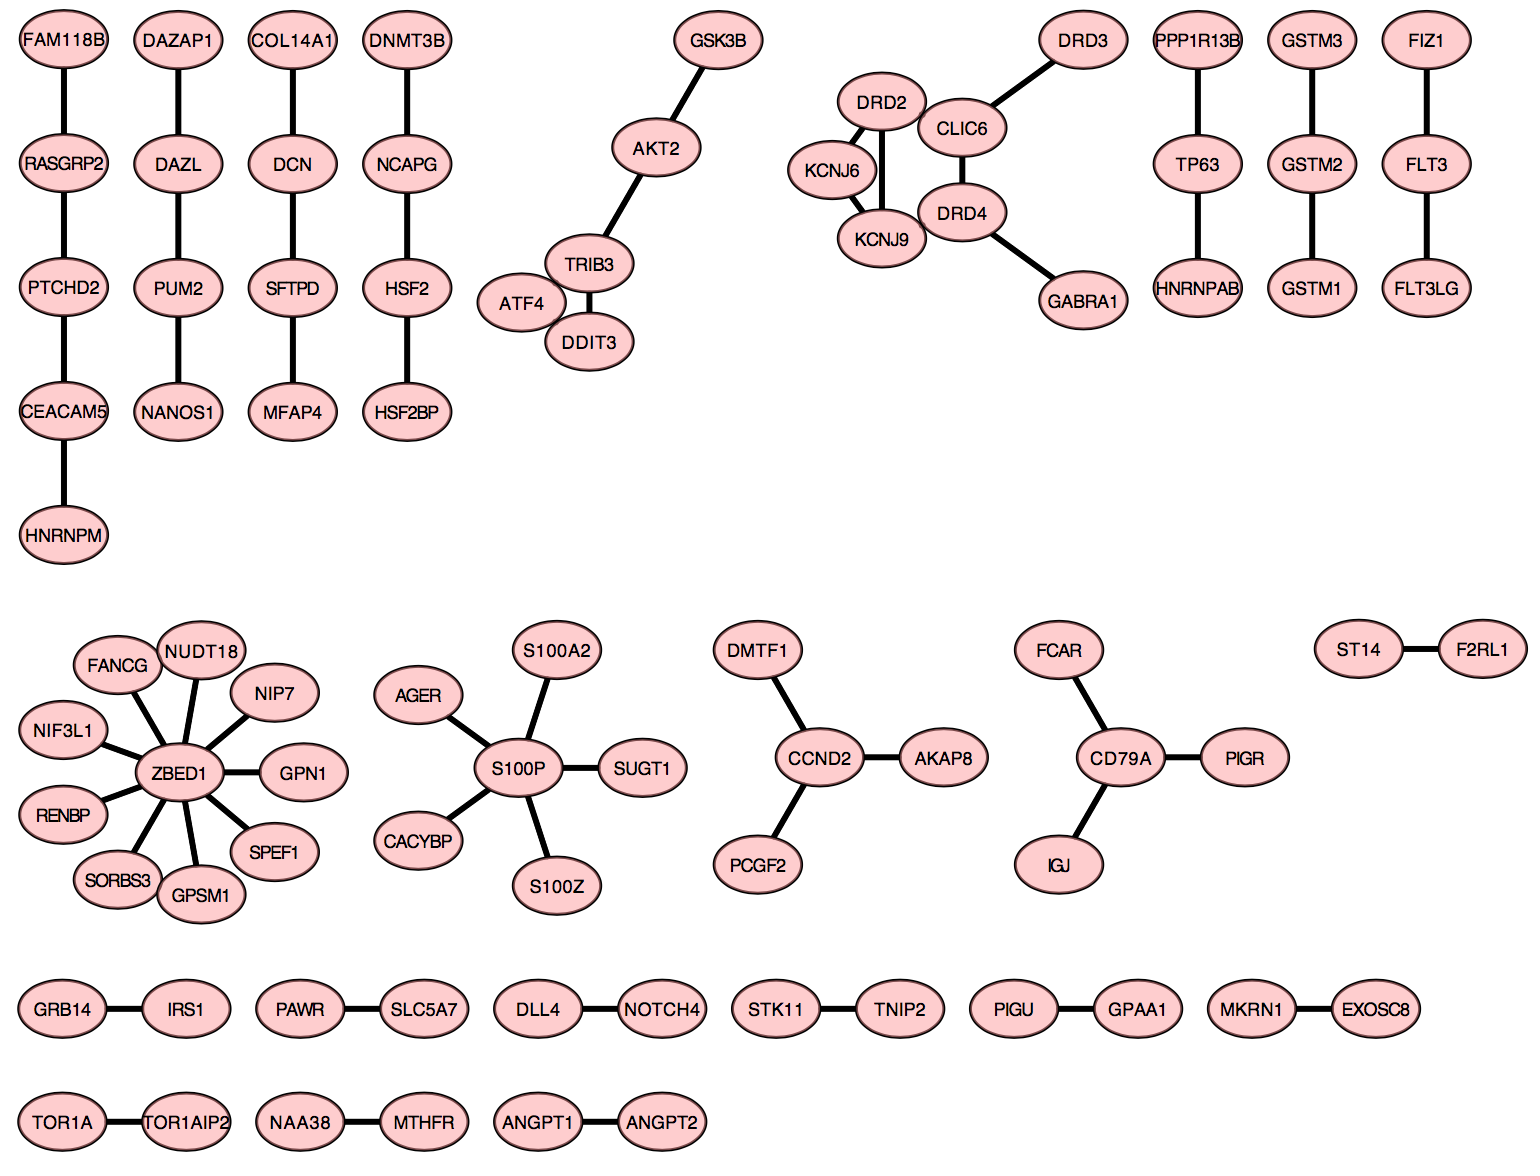
\includegraphics[width=\textwidth]{ch-wavelet/subnetworks_w-analysis_spec}
		\caption{Gene subnetworks identified by the wavelet-analysis method with spectral graph dual wavelets ($82$ genes connected out of $109$ selected).}
		\label{fig3:wanalysis}
	\end{subfigure}
	\caption{Gene subnetworks related to breast cancer survival identified by regularization methods using the METABRIC data and HPRD PPI network.}
	\label{fig3:subnetworks}
\end{figure}



It is interesting to investigate from a biological point of view the genes selected by our survival analysis for breast cancer using the METABRIC gene expression data and the HPRD PPI network, where the regularization parameter $\lambda$ and thus the number of genes selected is determined by cross-validation. In particular, we focus on comparing the three methods denoted by ``e-net'', ``laplasso (norm)'' and ``\wanaspec{}'' for the reminder of the section, each representing a class of methods. The network-free elastic net identified a total of $112$ genes, among which only $10$ genes are not isolated from one another on the HPRD PPI network that form $5$ connected gene pairs (Figure \ref{fig3:enet}). The network-based Laplacian lasso identified a total of $100$ genes, among which $10$ genes are connected and they coincide exactly with the the connected genes identified by the elastic net (Figure \ref{fig3:enet}). Our network-based wavelet-analysis method with spectral graph dual wavelets identified a total of $109$ genes, among which $82$ genes are connected that form $23$ gene modules of various sizes and shapes (Figure \ref{fig3:wanalysis}). We refer to the online supplements for the full list of genes selected by each method and in this study focus on the connected genes that form collaboratively functional gene modules.



The wavelet-based method is able to select more genes that form larger subnetworks than the other two methods. Specifically, there are two pairs of connected genes that are commonly selected by the three methods. First, while the other two methods detected the relation to cancer survival of GSTM2 and GSTM3 genes, the wavelet-based method was able to detect the involvement of three genes from the same gene family that are GSTM1, GSTM2 and GSTM3. In fact, glutathione metabolism is able to play both protective and pathogenic roles with respect to cancer \cite{Balendiran2004role,Wu2004Glutathione}, and the human GSTM gene family encodes the mu class of metabolic isoenzymes of glutathione S-transferase, consisting of five different but closely related isotypes GSTM1 to GSTM5. It has been reported that certain GSTM genes are correlated with the likelihood of breast cancer recurrence and functionally contribute prognostic information \cite{Kiefer2014Multiple}. In particular, GSTM1, which was detected only by the wavelet-based method, has been extensively studied in breast cancer risk especially due to its null genotype \cite{Roodi2004Association,Sull2004Glutathione}, but the absence of a functional GSTM1 enzyme in a null variant can be meaningfully compensated for by GSTM2 \cite{Bhattacharjee2013Functional}. Second, while the other two methods selected ZBED1 and SORBS3 genes simultaneously, the wavelet-based method detected through interactions documented in HPRD a star-shaped subnetwork in which the hub gene ZBED1 is centered around by $9$ other genes SORBS3, FANCG, GPSM1, NUDT18, SPEF1, NIP7, GPN1, RENBP, NIF3L1. This is in fact the largest subnetwork identified by the wavelet-based method, in which some genes are of particular interest. In fact, the ZBED1 gene encodes a protein which binds to DNA elements found in the promoter regions of a number of genes related to cell proliferation \cite{Matsukage2008DREDREF,Yamashita2007hDREF}. The FANCG gene,, which was detected only by the wavelet-based method, provides instructions for making a protein complex involved in the Fanconi anemia (FA) pathway responsible for DNA repair and it has been reported to directly interact with BRCA2 gene that plays an important role in homologous recombination repair and survival risk in breast cancer \cite{Hussain2003Direct,Wilson2008FANCG}.




Among the subnetworks identified exclusively by our wavelet-based method, some are of particular interest and the involvement of the connected genes in cancer biology was previously reported in literature. For example, an interesting subnetwork is composed of $7$ genes DRD2, DRD3, DRD4, CLIC6, KCNJ6, KCNJ9, GABRA1. In fact, the D2-like family of the dopamine receptors, encoded by genes DRD2, DRD3 and DRD4, are coupled to certain guanine nucleotide-binding proteins (G proteins) which directly inhibits adenylate cyclase activity and cyclic adenosine monophosphate (cAMP) formation \cite{Neves2002G}, and whose signaling has been linked to cancer progression and cancer risk \cite{Murphy2009Dopamine,Mao2015Dopamine} leading to many preclinical studies on the antitumor effects sought by antagonizing DRD2 signaling \cite{Pornour2015New,Hoeppner2015Dopamine}. Notably, all three genes DRD2, DRD3 and DRD4 are simultaneously selected due to their common interactor gene CLIC6. The second interesting subnetwork of interest is composed of $5$ genes AKT2, ATF4, DDIT3, GSK3B, TRIB3. In this subnetwork, three genes AKT2, ATF4 and DDIT3 are present in the mitogen-activated protein kinase (MAPK) signaling pathway whose relevance to cancer has been profoundly studied and we refer to \cite{Dhillon2007MAP} for an overview; three genes AKT2, ATF4 and GSK3B are found in the PI3K/Akt signaling pathway whose role in breast cancer has been reported in \cite{FresnoVara2004PI3KAkt,Paplomata2014PI3KAKTmTOR} for instance, and two genes AKT2 and GSK3B are included in the KEGG pathways in cancer. The third interesting subnetwork is a star-shaped gene module composed of $4$ genes CCND2, DMTF1, AKAP8, PCGF2. In fact, the hub gene CCND2 encodes cyclin D2, a protein belonging to a highly conserved family of cyclin proteins that control cell progression through regulating cell cycle. There exists an extensive body of literature on the role of D-type cyclins as a biomarker in cancer phenotype and progression, see \cite{Musgrove2011Cyclin} for a recent review. Connected to gene CCND2 is gene DMTF1 which encodes a cyclin D-binding myb-like transcription factor. DMTF1 was known for its tumor suppressive role linked to the regulation of many signaling pathways involving the tumor protein 53 (TP53) as well as CCND1, see \cite{Tian2017From} for a recent review. The last subnetwork worth special mention is the gene triplet of FLT3, FLT3LG and FIZ1, among which two genes FLT3LG and FLT3 are included in the KEGG pathways in cancer. The gene FLT3 encodes a class III receptor tyrosine kinase that regulates hematopoiesis whose role in the pathogenesis of acute myeloid leukemia (AML) in particular has been long recognized \cite{Levis2003FLT3}. Besides, FLT3LG, namely the FLT3 ligand, also plays a role in the immune response, and hence it was investigated in the pursuit of promising immuno-therapy against cancer by means of vaccine adjuvant \cite{Lynch1997FLT3,Kreiter2011FLT3}. Notably, gene FLT3 was selected by all three methods under consideration, but its connected gene FLT3LG was selected exclusively by the wavelet-based method.



\section{Discussion}
\label{sec3:discussion}



In the present chapter, we have studied network-based regularization methods under a predictive framework with linear models in order to incorporate relationships between features presumably encoded by a known network, and proposed to use network-based wavelet smoothing in order for subnetwork detection by structured feature selection. Notably, the proposed methods are essentially a class of penalty terms that are readily combined with any loss function appropriately chosen depending on the application in fitting linear models, and path-wise algorithms for solving the underlying optimization problems are straightforwardly available by modifying those solving the standard lasso. Finally, we demonstrated the proposed methods by performing survival analysis for breast cancer using METABRIC gene expression data guided by a PPI network obtained from HPRD. Results show that, compared to several state-of-the-art methods, the wavelet-analysis method with spectral graph dual wavelets, as a representative of wavelet-based methods, was able to improve the efficacy of gene selection in terms of stability, connectivity and interpretability, while achieving competitive performance of survival risk prediction. In particular, the wavelet-based method identified larger subnetworks involving more connected genes, and the relevance of many genes to breast cancer survival have been previously reported by independent studies.


Key insights into the superiority of network-based wavelet smoothing to other network-based regularization methods regarding feature selection lie in the properties of graph wavelets. Recall that graph wavelets are graph vectors that are localized on the graph and fully determined by the local structure of the graph. In particular, the construction of graph wavelets conceals an automated procedure of designating subnetworks whose location, size and shape are inherently specified by the underlying graph wavelets. When any graph vector is decomposed into a linear combination of graph wavelets, we obtain a new representation of the graph vector that are decorrelated and modularized with respect to graph wavelets. The idea of wavelet smoothing originates from seeking for a coefficient vector of the linear model that is sparse in its wavelet representation, and the modularized sparsity of the coefficient vector consequently enables direct identification of subnetworks adapted to optimizing the prediction. Contrariwise, the sparsity-inducing term for feature selection in the Laplacian lasso is a standard lasso term that regards features rather individually, despite that an additional Laplacian term controls the global smoothness of the coefficients and thus encourages features closer on the network to be selected simultaneously. Likewise, the spirit of feature selection for the graph fused lasso is indeed direct identification of subnetworks. This is achieved, however, through an estimate of the coefficient vector that is forced piece-wise constant over the network. Therefore, the resulting subnetwork is only data-adaptive but not adapted to the locally irregular structure of the network. Besides, when we expect that the relationships between features conform to the network structure, the compulsory constrain seems too strong an assumption that all features in each subnetwork should share exactly the same coefficient.


When performing network-based analysis of gene expression data, we highlighted the benefits of using a PPI network to guide gene selection related to breast cancer survival. An important issue is that our knowledge of protein-protein interaction is undoubtedly incomplete and the edges of the known biological network can possibly be subject to errors or misspecifications, especially when it comes to the biology of cancer mechanism. Future research of pressing need would be to investigate how sensitive the results are to perturbation of the network structure. A potentially helpful trick to improve our trust in the external knowledge provided by the network could be to adapt the given network to data by modifying edges from the network , for instance removing certain edges if the correlation of the expression levels between the two connected genes is very small. Another issue prior to employing network-based analysis is to decide which biological network to use, which in principle depends on domain expertise. In fact, the methods considered in this study, including the wavelet-based methods, can be applied with various biological networks such as coexpression networks. However, an open question is to compare the list of selected genes and detected subnetworks when guided by different biological networks or from different databases. Finally, we would like to point out that, despite the findings of this study, the rationale for network-guided genomic data analysis for improving prediction performance of breast cancer survival remains a controversial topic \cite{Staiger2013Current}. Comprehensive studies benchmarking the breast cancer survival analysis with more datasets, networks, regularization methods and prediction tasks, such as those that follow the evaluation pipeline of \cite{Staiger2013Current}, is called for in future research.


For the methods of network-based wavelet smoothing, many variants exist and have been empirically tested in the numerical experiments of this study, raising a few points worth discussion and further investigation. First, we observed distinct performance with respect to which version of graph Laplacian (normalized or non-normalized) is used for the construction of spectral graph wavelets. In fact, there are many theoretical guarantees that favor the normalized Laplacian \cite{Chung1997Spectral} but a debate is ongoing over which version should be used in practice. Despite that we opted for the non-normalized Laplacian by default, we do not conclude definitively on the choice of Laplacian that is better suited for the construction of spectral graph wavelets integrated in network-based wavelet smoothing. Second, this study provides an empirical benchmark comparing the performance of two particular types of graph wavelets, that are spectral graph wavelets and lifting-based graph wavelets. Evidences from all experiments strongly advocate the use of spectral graph wavelets over lifting-based graph wavelets, and the substantially deficient performance of latter is somewhat surprising. In fact, if data are time series that reside on 1-dimensional chain graph, it has been proven that any discrete wavelet transform with all classical wavelet filter banks can be factored into a sequence of lifting steps \cite{Daubechies1998Factoring}. Therefore, it calls for theoretical studies that provide a unifying overview of different techniques of performing wavelet transform on general graphs. Third, we proposed to use two approaches to wavelet smoothing, namely the synthesis approach \eqref{eq3:synthesis} and the analysis approach \eqref{eq3:analysis}. Despite the similarity in their mathematical formulation, the motivation underlying both approaches differ fundamentally. The synthesis approach seeks a reconstruction of the coefficient vector as a sparse combination of graph wavelets, while the analysis approach aspires to build sparse predictive models on the wavelet-transformed feature data. Our real-data experiments on survival analysis for breast cancer particularly suggest that the analysis approach usually outperforms the synthesis approach, as observed also by \cite{Elad2007Analysis} concerning applications in signal processing.


There are many interesting extensions of the current work. One direction would be to perform wavelet smoothing on directed graphs or graphs with some edge attributes. This is particularly relevant when we would like to explore relationships between features associated with irreversible direction and meaningful attributes. For example, in a signaling pathway network, each edge is associated with a direction (indicating cell signaling is transduced from one gene to another but cannot be reversed) as well as an annotated type of interaction (activation or inhibition). Another direction would be to explore the possibility of adopting, besides graph wavelet transform, other types of localized or multiscale transforms specifically designed to analyze data on graphs, such as windowed graph Fourier transform \cite{Shuman2012windowed} or multiscale graph pyramid transform \cite{Shuman2016multiscale}. In particular when the two directions engage in one application, deeper understanding of the network utilized can be enlightening for the applicability of the methods and transforms employed.

\cleardoublepage

\chapter{Signaling Pathway Activities Improve Prognosis for Breast Cancer}
\label{chap:hipathia}

\begin{chapabstract}{Abstract:}
With the advent of high-throughput technologies for genome-wide expression profiling, a large number of methods have been proposed to discover gene-based signatures as biomarkers to guide cancer prognosis. However, it is often difficult to interpret the list of genes in a prognostic signature regarding the underlying biological processes responsible for disease progression or therapeutic response. A particularly interesting alternative to gene-based biomarkers is mechanistic biomarkers, derived from signaling pathway activities, which are known to play a key role in cancer progression and thus provide more informative insights into cellular functions involved in cancer mechanism. In this chapter, we demonstrate that a pathway-level feature, such as the activity of signaling circuits, outperform conventional gene-level features in prediction performance in breast cancer prognosis. We also show that the proposed classification scheme can even suggest, in addition to relevant signaling circuits related to disease outcome, a list of genes that do not code for signaling proteins whose contribution to cancer prognosis potentially supplements the mechanisms detected by pathway analysis. This study is under submission as joint work with Marta R. Hidalgo, Cankut \c{C}ubuk, Alicia Amadoz, Jos\'{e} Carbonell-Caballero, Jean-Philippe Vert, Joaqu\'{i}n Dopazo \cite{Jiao2017Signaling}.
\end{chapabstract}
\vskip 0.2in
\begin{chapabstract}{R�sum� :}
Avec l'av�nement des technologies � haut d�bit pour le profilage d'expression g�nomique, un grand nombre de m�thodes ont �t� propos�es pour d�couvrir des signatures bas�es sur les g�nes en tant que biomarqueurs pour aider le pronostic du cancer. Cependant, il est souvent difficile d'interpr�ter la liste des g�nes dans une signature pronostique et ce � cause des processus biologiques sous-jacents responsables de la progression de la maladie ou de la r�ponse th�rapeutique. Une alternative particuli�rement int�ressante aux biomarqueurs g�n�tiques est le biomarqueur m�canique, d�riv� des activit�s des voies de signalisation, qui est connu pour jouer un r�le cl� dans la progression du cancer et ainsi fournir des informations plus pertinentes sur les fonctions cellulaires impliqu�es dans le m�canisme du cancer. Dans ce chapitre, nous d�montrons que les variables issues du r�seau, comme l'activit� des circuits de signalisation, surpasse les variables classiques au niveau du g�ne en termes de pr�diction du pronostic du cancer du sein. Nous montrons �galement que notre m�thode de classification permet de proposer, en plus de la pertinence des variables issues du r�seau li�es au r�sultat de la maladie, une liste des g�nes qui ne codent pas de prot�ines de signalisation dont la contribution au pronostic du cancer peut compl�ter les m�canismes d�tect�s par l'analyse du r�seau. Cette �tude est soumise en collaboration avec Marta R. Hidalgo, Cankut \c{C}ubuk, Alicia Amadoz, Jos\'{e} Carbonell-Caballero, Jean-Philippe Vert, Joaqu\'{i}n Dopazo \cite{Jiao2017Signaling}.
\end{chapabstract}

\section{Introduction}
\label{sec4:intro}

Over the past decades, many efforts have been addressed to the identification of gene-based signatures to predict  patient prognosis using gene expression data \cite{Veer2002Gene, Paik2004multigene, Wang2005Gene, Sotiriou2009Gene, Reis-Filho2011Gene}. Despite the success of its use, gene expression signatures have not been exempt of problems \cite{Ein-Dor2006Thousands, Iwamoto2010Predicting}. Specifically, one major drawback of multi-gene biomarkers is that they often lack proper interpretation in terms of mechanistic link to the fundamental cell processes responsible for disease progression or therapeutic response \cite{Veer2008Enabling, Dopazo2010Functional}. Actually, it is increasingly recognized that complex traits, such as disease or drug response, are better understood as alterations in the operation of functional modules caused by different combinations of gene perturbations \cite{Barabasi2004Network, Oti2007modular, Barabasi2011Network}. To address this inherent complexity different methodologies have tried to exploit several functional module conceptual representations, such as protein interaction networks or pathways, to interpret gene expression data within a systems biology context \cite{Barabasi2011Network, Vidal2011Interactome, Hood2013Systems, Fryburg2014Systems}.

Here we focus on consulting prior knowledge of signaling pathways to guide cancer prognosis. It is well understood that cell signaling is a system of within-cell communication and signal transduction process between gene products, mostly proteins, that coordinates cell activities to perceive and correctly respond to microenvironment, resulting in signaling pathways that form a particular type of functional gene modules and play a key role in disease progression (Figure \ref{fig4:cellsignaling}). Consequently as a tempting solution to the limitation of conventional analysis at the level of individual genes, analysis at the level of pathways renders great interest in providing informative insights into cellular functions that facilitates understanding of the disease mechanism. Actually, it has recently been shown that the pathway-level representation generates clinically relevant stratifications and outcome predictors for glioblastoma and colorectal cancer \cite{Drier2013Pathway} and also breast cancer \cite{Livshits2015Pathway}. Moreover, mathematical models of the activity of a pathway have demonstrated a significantly better association to poor prognosis in neuroblastoma patients than the activity of their constituent genes, including MICN, a conventional biomarker \cite{Fey2015Signaling}. This observation has recently been extended to other cancers \cite{Hidalgo2017High} and to the prediction of drug effects \cite{Amadoz2015Using}.

\begin{figure}[!htbp]
	\centering
	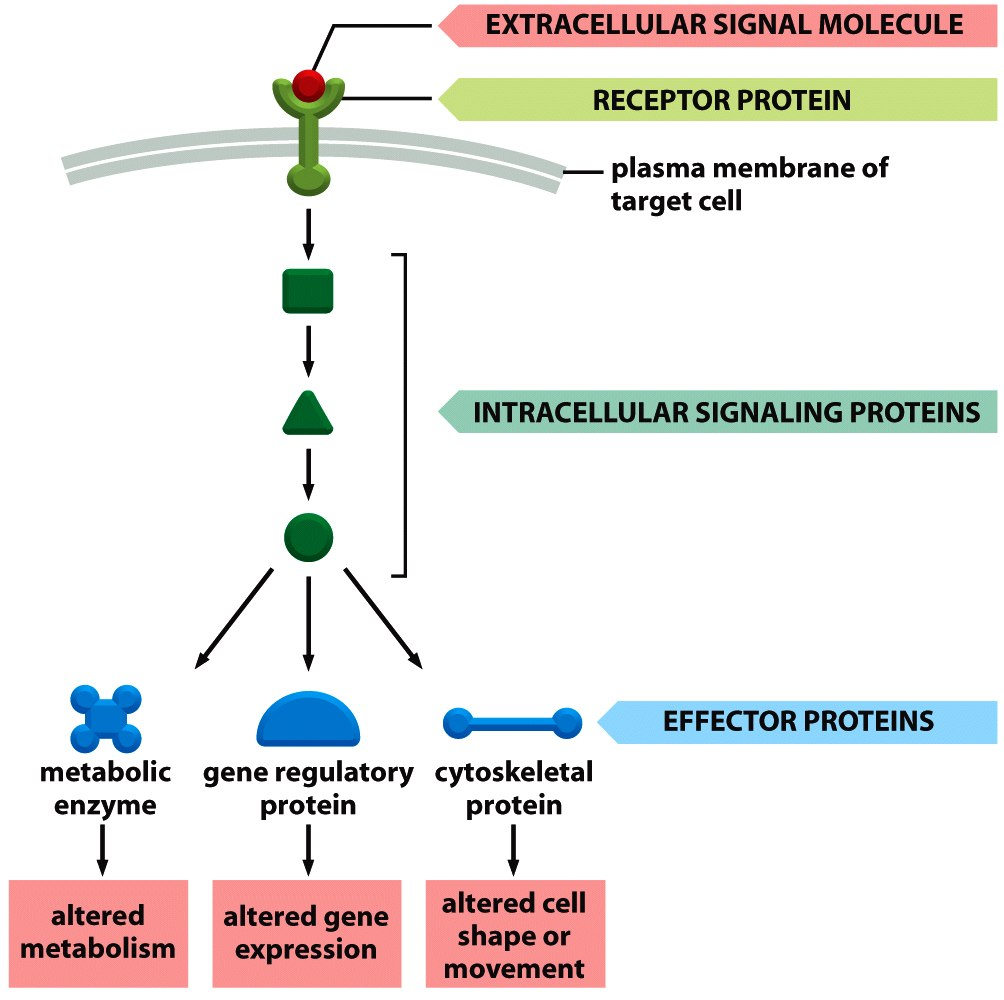
\includegraphics[width=0.6\textwidth]{ch-hipathia/figure/signaling_pathway}
	\caption{An illustration of cell signaling process. Typically the signal transduction begins at receptor proteins that receive molecular stimuli from cell microenvironment and ends at effector proteins that execute specific actions in response to the stimulation.}
	\label{fig4:cellsignaling}
\end{figure}

Given that the inferred activity of the pathway should be closely related to its cellular mechanism for disease progression, its use to guide cancer prognosis seems promising. Recently, a number of pathway activity inference methods have been proposed \cite{Hidalgo2017High, Jacob2012More, Li2015Subpathway, Martini2013Along}. Here, we use the \textit{hiPathia} method proposed in \cite{Hidalgo2017High}, as it has been demonstrated to have a superior performance finding significant associations of specific circuit\footnote{Circuits can be understood as sub-pathways with specific  structure in stimulus-response signaling pathways, while definitions are postponed to Section \ref{sec4:hipathia}.} activities, directly responsible for triggering the prominent cancer hallmarks \cite{Hanahan2011Hallmarks}, to patient survival. This method recodes gene expression values into measurements of signaling circuit activities that ultimately account for cell responses to specific stimuli. Such activity values can be considered multigenic mechanistic biomarkers that can be used as features for cancer prognosis.

In this chapter, we demonstrate that the activity of signaling circuits yields comparable or even better prediction in breast cancer prognosis than the expression of individual genes, while detected mechanistic biomarkers enjoy the compelling advantage of readily available interpretation in terms of the corresponding cellular functions they trigger. Moreover, we show that the proposed prediction scheme can even suggest, in addition to interesting signaling circuits related to disease outcome, a list of genes that do not code for signaling proteins whose contribution to cancer prognosis potentially supplements the mechanism included in the pathways modeled. All numerical results are produced with \texttt{R} and codes for reproducing the experiments are available in the online supplementaries at \url{https://github.com/YunlongJiao/hipathiaCancerPrognosis}.




\section{Methods}
\label{sec4:methods}

\subsection{Data Source and Processing}
\label{sec4:data}

Our interest in this study lies in predicting the overall survival outcome of breast cancer patients making use of gene expression data. The breast cancer gene expression and survival data here were downloaded from The Cancer Genome Atlas (TCGA), release No. 20 of the International Cancer Genome Consortium (ICGC) data portal under project name BRCA-US\footnote{More information can be found at \url{https://dcc.icgc.org/releases/release_20/Projects/BRCA-US}.}. This dataset provides the RNA-seq counts of 18,708 genes for 879 tumor samples in which we also have records of the vital status of corresponding donors, namely the overall survival outcome of the cancer patients being alive or deceased at the end of clinical treatment (Table \ref{tab4:survival}). This way we deal with a binary classification problem distinguishing good vs poor prognosis based on gene expression measurements of breast tumor samples. Since TCGA cancer data are collected from different origins and underwent different management processes, non-biological experimental variations, commonly known as batch effect, associated to Genome Characterization Center (GCC) and plate ID must be removed from the RNA-seq data. The COMBAT method \cite{Johnson2007Adjusting} was used for this purpose. We then applied the trimmed mean of M-values normalization method (TMM) method \cite{Robinson2010scaling} for data normalization which is essential in applying the \textit{hiPathia} method. The resulting normalized values were finally entered to the pathway analysis method.

\begin{table}[!htbp]
	\centering
	\caption{Summary of survival outcome of the breast cancer patients in the TCGA dataset.}
	\begin{tabular}{|l|l|r|r|}
		\hline
		\textbf{Donor vital status} & \textbf{Pseudo label} & \textbf{No. of samples} & \textbf{Percentage} \\
		\hline
		Deceased (poor prognosis) & Positive & 124 & 14.1\% \\\hline
		Alive (good prognosis) & Negative & 755 & 85.9\% \\\hline
		\multicolumn{2}{|r|}{\textbf{Total}} & 879 & 100.0\% \\
		\hline
	\end{tabular}
	\label{tab4:survival}
\end{table}

In order to explore the potential of utilizing external knowledge of cell signaling to enhance prognosis, we consulted Kyoto Encyclopedia of Genes and Genomes (KEGG) repository \cite{Kanehisa2012KEGG} to retrieve relationships between proteins within signaling pathways. A total of 60 KEGG pathways were used (Table \ref{tab4:kegg}), comprehending 2,212 gene products that participate in 3,379 nodes. Note that most gene products are proteins, and two types of nodes are defined in KEGG: plain nodes which may contain one or more proteins and complex nodes. These pathways each compose into a directed network where nodes are connected with edges labeled by either activation or inhibition depending on the action in transmitting signals along the path. In particular, input nodes that have no incoming edges represent receptor proteins which receive molecular stimuli from cell microenvironment, and output nodes that have no outgoing edges represent effector proteins which carry out specific cellular functions. We will elaborate in the following subsection on how to decompose the complex structure of KEGG pathways in order to effectively apply the \textit{hiPathia} method.

\begin{center}
	\begin{longtable}[H]{|l|l|}
	\caption{The 60 KEGG pathways for which signaling activity is modeled.}
	\label{tab4:kegg}\\
		
		\hline \multicolumn{1}{|l|}{\textbf{KEGG identifier}} & \multicolumn{1}{l|}{\textbf{Pathway name}} \\ \hline 
		\endfirsthead
		
		\multicolumn{2}{c}%
		{{\tablename\ \thetable{} -- continued from previous page}} \\
		\hline \multicolumn{1}{|l|}{\textbf{KEGG identifier}} & \multicolumn{1}{l|}{\textbf{Pathway name}} \\ \hline 
		\endhead
		
		\multicolumn{2}{|r|}{\textit{Continued on next page}} \\ \hline
		\endfoot
		
		\hline
		\endlastfoot
		
		hsa04014 &
		Ras signaling pathway \\\hline
		hsa04015 &
		Rap1 signaling pathway \\\hline
		hsa04010 &
		MAPK signaling pathway \\\hline
		hsa04012 &
		ErbB signaling pathway \\\hline
		hsa04310 &
		Wnt signaling pathway \\\hline
		hsa04330 &
		Notch signaling pathway \\\hline
		hsa04340 &
		Hedgehog signaling pathway \\\hline
		hsa04350 &
		TGF-beta signaling pathway \\\hline
		hsa04390 &
		Hippo signaling pathway \\\hline
		hsa04370 &
		VEGF signaling pathway \\\hline
		hsa04630 &
		Jak-STAT signaling pathway \\\hline
		hsa04064 &
		NF-kappa B signaling pathway \\\hline
		hsa04668 &
		TNF signaling pathway \\\hline
		hsa04066 &
		HIF-1 signaling pathway \\\hline
		hsa04068 &
		FoxO signaling pathway \\\hline
		hsa04020 &
		Calcium signaling pathway \\\hline
		hsa04071 &
		Sphingolipid signaling pathway \\\hline
		hsa04024 &
		cAMP signaling pathway \\\hline
		hsa04022 &
		cGMP-PKG signaling pathway \\\hline
		hsa04151 &
		PI3K-Akt signaling pathway \\\hline
		hsa04152 &
		AMPK signaling pathway \\\hline
		hsa04150 &
		mTOR signaling pathway \\\hline
		hsa04110 &
		Cell cycle \\\hline
		hsa04114 &
		Oocyte meiosis \\\hline
		hsa04210 &
		Apoptosis \\\hline
		hsa04115 &
		p53 signaling pathway \\\hline
		hsa04510 &
		Focal adhesion \\\hline
		hsa04520 &
		Adherens junction \\\hline
		hsa04530 &
		Tight junction \\\hline
		hsa04540 &
		Gap junction \\\hline
		hsa04611 &
		Platelet activation \\\hline
		hsa04620 &
		Toll-like receptor signaling pathway \\\hline
		hsa04621 &
		NOD-like receptor signaling pathway \\\hline
		hsa04622 &
		RIG-I-like receptor signaling pathway \\\hline
		hsa04650 &
		Natural killer cell mediated cytotoxicity \\\hline
		hsa04660 &
		T cell receptor signaling pathway \\\hline
		hsa04662 &
		B cell receptor signaling pathway \\\hline
		hsa04664 &
		Fc epsilon RI signaling pathway \\\hline
		hsa04666 &
		Fc gamma R-mediated phagocytosis \\\hline
		hsa04670 &
		Leukocyte transendothelial migration \\\hline
		hsa04062 &
		Chemokine signaling pathway \\\hline
		hsa04910 &
		Insulin signaling pathway \\\hline
		hsa04922 &
		Glucagon signaling pathway \\\hline
		hsa04920 &
		Adipocytokine signaling pathway \\\hline
		hsa03320 &
		PPAR signaling pathway \\\hline
		hsa04912 &
		GnRH signaling pathway \\\hline
		hsa04915 &
		Estrogen signaling pathway \\\hline
		hsa04914 &
		Progesterone-mediated oocyte maturation \\\hline
		hsa04921 &
		Oxytocin signaling pathway \\\hline
		hsa04919 &
		Thyroid hormone signaling pathway \\\hline
		hsa04916 &
		Melanogenesis \\\hline
		hsa04261 &
		Adrenergic signaling in cardiomyocytes \\\hline
		hsa04270 &
		Vascular smooth muscle contraction \\\hline
		hsa04722 &
		Neurotrophin signaling pathway \\\hline
		hsa05200 &
		Pathways in cancer \\\hline
		hsa05231 &
		Choline metabolism in cancer \\\hline
		hsa05202 &
		Transcriptional misregulation in cancer \\\hline
		hsa05205 &
		Proteoglycans in cancer \\\hline
		hsa04971 &
		Gastric acid secretion \\\hline
		hsa05160 &
		Hepatitis C
	\end{longtable}
\end{center}

\subsection{Modeling Framework for Signaling Pathways}
\label{sec4:hipathia}

We applied the \textit{hiPathia} method\footnote{Available as an \texttt{R} package at \url{https://github.com/babelomics/hipathia} and via a web interface at \url{http://hipathia.babelomics.org/}.} proposed by \cite{Hidalgo2017High} in pursuit of modeling signaling activity. Overall, \textit{hiPathia} is a method that estimates the level of activity within a signaling circuit by modeling cell signaling process in order to recode gene expression values into measurements that ultimately account for cell responses caused by pathway activities. Essentially the \textit{hiPathia} method computes an activity value for each stimulus-response sub-pathway within signaling circuits. This way, the sub-pathways which associate naturally with cell functionalities can be considered as mechanistic features that are modularized from multigenic signatures, and their activity values connected to the activation or deactivation of specific cellular functions thus provide quantitative clues to understand disease mechanisms when further related to phenotypes of interest such as cancer survival.

Recall that in cell signaling process represented in KEGG pathways, cell signal arrives to an initial input node and starts to transmit along any path following the direction of the edges until it reaches an output node that finally triggers a cellular action. In particular, from different input nodes the signal may follow different routes to reach different output nodes. Within the modeling context, a \textit{circuit} is naturally defined as all possible routes the signal can traverse to be transmitted from a particular input node to a particular output node (Figure \ref{fig4:pathway}, A). A total of 6,101 circuits are identified and modeled in this study. Now we take efforts to describe first how \textit{hiPathia} estimates the signaling activity of a circuit.

\begin{figure}[!htbp]
\centering
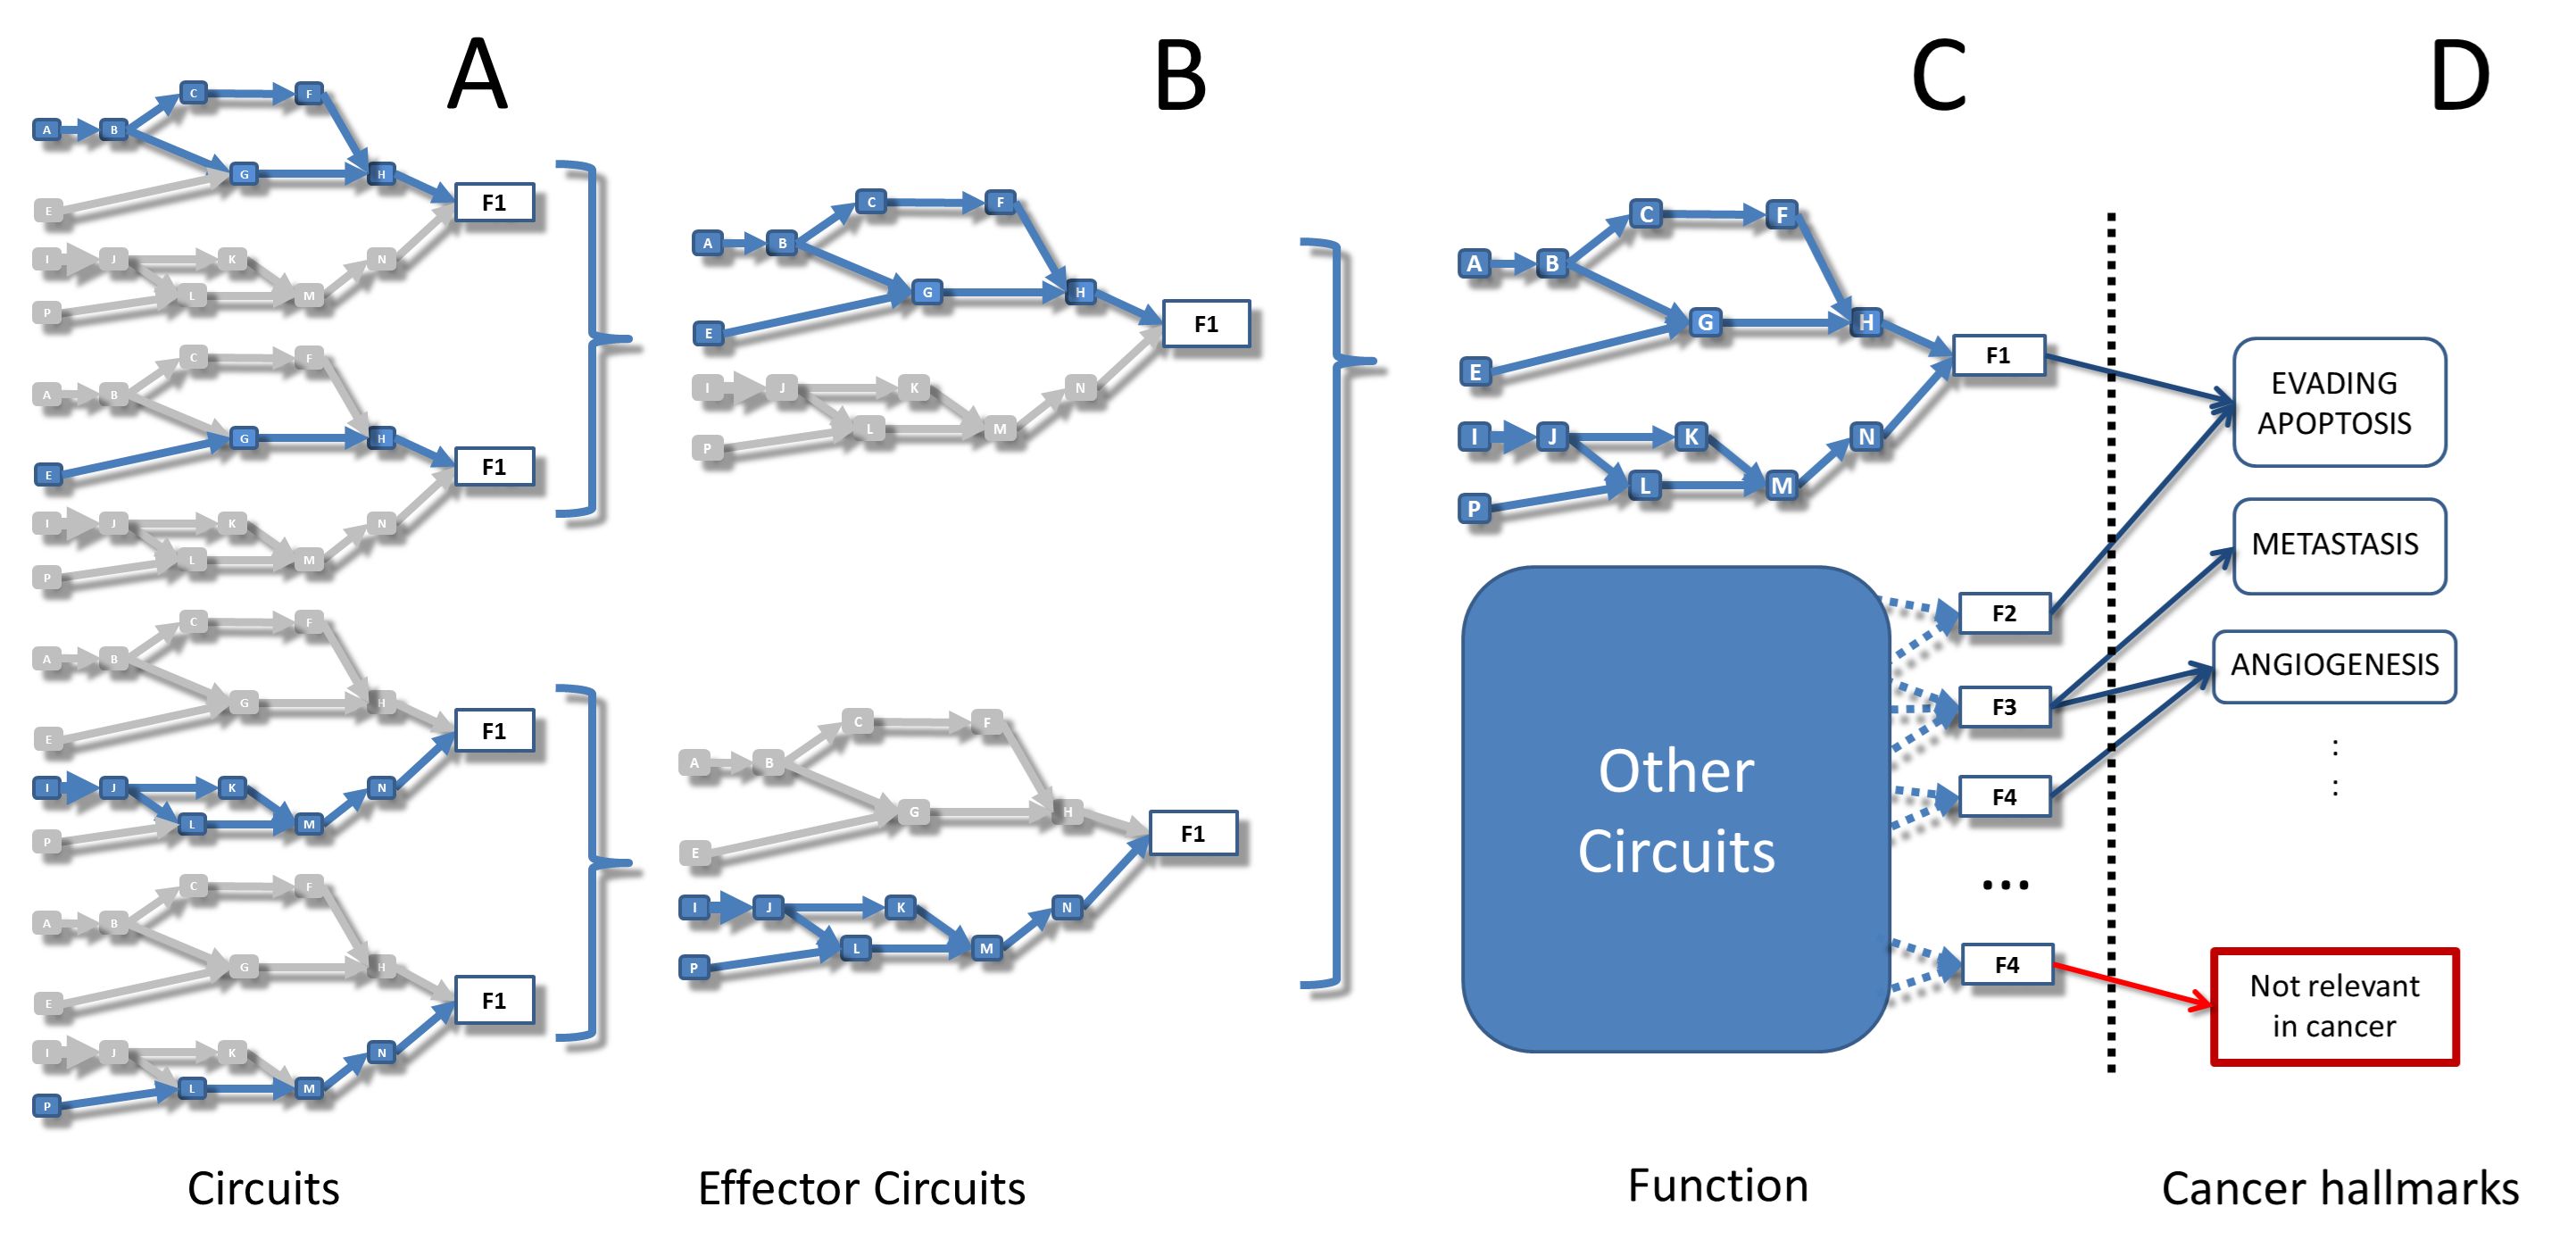
\includegraphics[width=\textwidth]{ch-hipathia/figure/pathway}
\caption{The different levels of abstraction within pathways: A) Circuits that communicate one receptor to one effector; B) Effector circuits that communicate all the receptors that signal a specific effector; C) Function circuits that collect the signal from all the effectors that trigger a specific function (according to UniProt or GO keywords); D) Cancer hallmarks, a sub-selection of only those functions related to cancer hallmarks.}
\label{fig4:pathway}
\end{figure}

In a signaling circuit, the transmission of the signal depends on the integrity of the chain of nodes that connect the receptor to the effector and the capability of transmitting signals of each node involved intuitively depends on two folds: the abundance of the proteins corresponding to that node and its activity status due to the interaction with its parent nodes. First, we need to estimate a value for each node in the pathways in regard to the presence of proteins involved in the node. Following the convention of \cite{Bhardwaj2005Correlation, Efroni2007Identification, Montaner2009Gene, Sebastian-Leon2014Understanding}, the presence of the mRNA (the normalized RNA-seq counts rescaled between 0 and 1) is taken as a proxy for the presence of the proteins involved in each node. Notably, for different types of nodes defined in KEGG, the value of a plain node in the pathways is defined as the ninetieth percentile of the values of the proteins contained, and the value of a complex node is taken as the minimum value of the proteins contained (the limiting component of the complex). Then, the degree of integrity of the circuit is estimated by modeling the signal flow across it, transmitting node-by-node following the path while its intensity value gets propagated along the way taking into account the current node value and the intensity of the signals arriving to it. Specifically, we initialize an incoming signal of intensity value of $1$ received by the input (receptor) node of the circuit, and then for each node $n$ of the circuit, the signal value $s_n$ is updated by the following rule:
$$
s_n = v_n \cdot \left( 1 - \prod_{a \in A_n} (1-s_a) \right) \cdot \prod_{i \in I_n} (1-s_i) \,,
$$
where $A_n$ denotes the set of signals arriving to the current node $n$ from activation edges, $I_n$ denotes the set of signals arriving to the current node $n$ from inhibition edges, and $v_n$ is the (normalized) value of the current node $n$. In case of loops present in the circuit, a node may be visited multiple times, until the difference in the updates of the signal value at that node is below certain threshold, before the signal exits the loop and continues to propagate down the cascade. Finally, the activity value for the circuit is defined by the signal intensity transmitted through the last (effector) protein of the circuit which quantifies the cell function ultimately activated by the circuit. See Figure \ref{fig4:hipathia} for an example of deducing the activity value of an artificial circuit by the \textit{hiPathia} method.

\begin{figure}[!htbp]
	\centering
	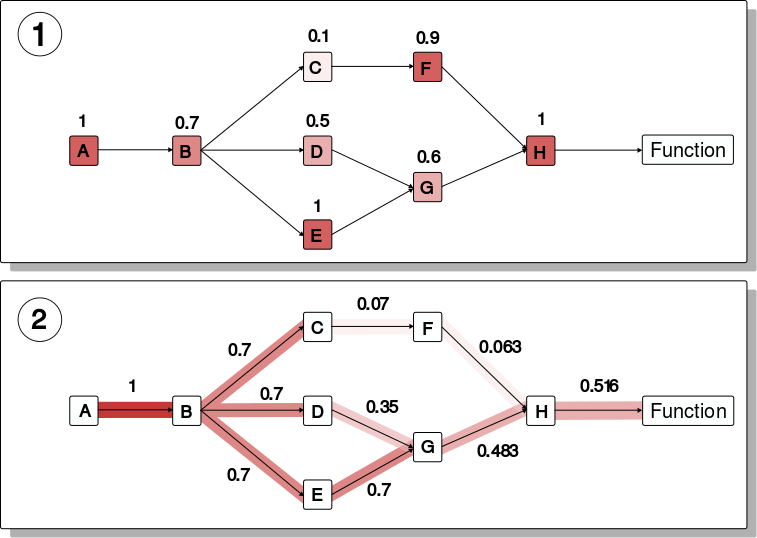
\includegraphics[width=0.6\textwidth]{ch-hipathia/figure/pretty_algorithm2}
	\caption{An example of computing the activity value of an artificial circuit by the \textit{hiPathia} method. In Step 1, node values are derived from the normalized mRNA measurements. In Step 2, signal is propagated along the path while its intensity value gets updated according to the rule of the \textit{hiPathia} method. Finally, The signal value attained after the last protein is visited accounts for the signaling activity of the circuit.}
	\label{fig4:hipathia}
\end{figure}

Besides, the \textit{hiPathia} method straightforwardly allows to explore pathway-level analysis at different levels of abstraction by applying to different notions of signaling circuits. As the output nodes at the end of circuits are the ultimate responsible to carry out specific cellular actions, an \textit{effector circuit} is defined from a functional viewpoint as a higher-level signaling entity that compose all circuits ending at the same output node (Figure \ref{fig4:pathway}, B). When applied to an effector circuit, the \textit{hiPathia} method returns the joint intensity of the signal arriving to the corresponding effector node. Furthermore, the known functions triggered in cell by each effector protein can be derived from their functional annotations. Here we use UniProt \cite{Consortium2015UniProt} and Gene Ontology (GO) \cite{Consortium2015Gene} annotations. Finally, inferred signaling activity values of those effector circuits ending at proteins with the same annotated functions are averaged to quantify the activity of the function realized in cell. This way we obtain estimated activity values directly connected to a list of cellular functions (Figure \ref{fig4:pathway}, C). Figure \ref{fig4:pathway} depicts the different levels of abstraction from circuits, to effector circuits and finally functions. Eventually for the sake of interpretation, a subset of curated functions can be used for a specific scenario in which the relevant functions are known to interpret the cancer biology, for which we use cancer hallmarks \cite{Hanahan2011Hallmarks} (Figure \ref{fig4:pathway}, D).

\subsection{Cancer Prognosis with Inferred Signaling Pathway Activity}
\label{sec4:prognosis}

In this study, we are interested in comparing the prognostic power of pathway-level mechanistic features and gene-based features, both separately and in combination, in order to distinguish good vs poor prognosis. Using the \textit{hiPathia} method, we recoded the list of gene expression values of each tumor sample into the corresponding lists of signaling activity values for the three levels of abstraction: circuits, effector circuits and functions, as described in UniProt and GO annotations. Therefore for each tumor sample, we end up with a profile of gene expression, a profile of circuit signaling activity, a profile of effector circuit signaling activity, a profile of UniProt-based cellular function activity and a profile of GO-based cellular function activity. These profiles are sample-specific, or so-called \textit{personalized}, profiles that can be straightforwardly used as prognostic features for cancer prognosis following any off-the-shelf classification algorithm. Note that pathway-level profiles are derived with no regard to any information provided by the genes whose products do not participate in cell signaling, and the prognostic power of pathway-level profiles may thus be limited by the coverage of genes in known biological pathways. In order to understand the relative contribution to the pathway-level profiles and gene-level profiles to the accurate separation between good vs poor prognosis, we devised 4 artificial profiles: path-gene expression profile containing only genes that are involved in the KEGG signaling pathways, other-gene expression profile containing only genes that are absent from the KEGG pathways, a combined profile consisting of signaling activity of effector circuits and expression of other-genes, and a combined profile consisting of signaling activity of circuits and expression of other-genes. Thus we obtained a total of 9 types of profiles (detailed in Table \ref{tab4:profile}).

\begin{table}[!htbp]
	\centering
	\caption{Summary of 9 different types of profiles used as predictive features for breast cancer prognosis.}
	\renewcommand{\arraystretch}{1.3}
	\begin{tabular}{|p{2.6cm}|p{3.5cm}|>{\raggedleft\arraybackslash}p{1.6cm}|m{4.8cm}|}
		\hline
		\textbf{Alias} & \textbf{Profile type} & \textbf{No. of features} & \textbf{Analysis level} \\\hline
		\textit{fun.vals} & UniProt-based functions & 81 & \multirow{2}{*}{\parbox{4.5cm}{\raggedright Pathway-level cellular function values}} \\
		\textit{go.vals} & GO-based functions & 370 &  \\
		\hline
		\textit{eff.vals} & Effector circuits & 1,038 & \multirow{2}{*}{\parbox{4.5cm}{\raggedright Pathway-level signaling activity values}} \\
		\textit{path.vals} & Circuits & 6,101 &  \\
		\hline
		\textit{path.genes.vals} & Path-genes & 2,212 & \multirow{3}{*}{\parbox{4.5cm}{\raggedright Gene-level expression values}} \\
		\textit{other.genes.vals} & Other-genes & 16,496 &  \\
		\textit{genes.vals} & All genes & 18,708 &  \\
		\hline
		\textit{eff.and.other.-genes.vals} & Effector circuits and other-genes & 17,534 & \multirow{2}{*}{\parbox{4.8cm}{\raggedright Combination of pathway-level signaling activity values and gene-level expression values}} \\
		\textit{path.and.other.-genes.vals} & Circuits and other-genes & 22,597 &  \\
		\hline
	\end{tabular}
	\label{tab4:profile}
\end{table}

From the viewpoint of machine learning, this study is formulated as a typical binary classification problem where we determine a positive or negative pseudo label for each sample. Based on the data available in this study (Table \ref{tab4:survival}), we perform a 5-fold cross-validation repeated 10 times on the dataset and report the mean performance over the $5 \times 10 = 50$ splits to assess the prognostic power for each type of profile. The performance is evaluated by the Area Under the ROC Curve (AUROC) criteria \cite{Sing2005ROCR}. Note that usually a classifier returns a continuous prediction between 0 and 1 for each sample denoting the probability of that sample being in the positive class rather than in the negative class, and then assigns either label to the sample according to some cutoff value thresholding the prediction. AUROC is a cutoff-free score that measures the probability that the classifier will score a randomly drawn positive sample higher than a randomly drawn negative sample.

In this study, we considered a total of 12 classification algorithms as candidate classifiers, most of which are state-of-the-art (Table \ref{tab4:classifier}). When we assess the prognosis performance for a specific type of profile on a specific (external) cross-validation split of the data, we perform an internal 5-fold cross-validation on the training set to determine which classifier returns the highest cross-validated performance and the best classifier is then used on the test set to obtain the performance score. The rationale behind the nested cross-validation is that, although any classification algorithm from the machine learning literature can be used to discriminate good vs poor prognosis with any profile type considered as predictive features, in practice, however, we do not have a definitive concept of which classifier suits the best universally for all types of profiles. In other words, it will be a confusing factor if we predetermine just one classifier throughout the study. In fact, the underlying hypotheses of different classifiers vary, for instance linear or non-linear relationships can be assumed between features and labels, and some classifiers can be particularly sensitive to the presence of a large number of noisy features. As a consequence, the procedure of choosing the best suited algorithm for different types of profiles by a nested cross-validation guarantees that the prediction performance is evaluated in an impartial fashion.

\begin{table}[!htbp]
	\centering
	\caption{The 12 candidate classifiers used to discriminate prognosis classes for breast tumor samples.}
	\renewcommand{\arraystretch}{1.3}
	\begin{tabularx}{\textwidth}{|l|X|X|}
		\hline
		\textbf{Alias} & \textbf{Classifier} & \textbf{Reference} \\\hline
		\textit{LDA} & Linear discriminant analysis & \cite{Venables2002Modern, Ripley2007Pattern} \\\hline
		\textit{LogitLasso} & L1-regularized logistic regression & \cite{Friedman2010Regularization} \\\hline
		\textit{LinearSVM} & Support Vector Machines with linear kernel & \cite{Chang2011LIBSVM} \\\hline
		\textit{RadialSVM} & Support Vector Machines with Gaussian RBF kernel & \cite{Chang2011LIBSVM} \\\hline
		\textit{KendallSVM} & Support Vector Machines with Kendall kernel & \cite{Zeileis2004kernlab, Jiao2015Kendall} \\\hline
		\textit{KNN} & $k$-nearest neighbor classifier & \cite{Venables2002Modern, Ripley2007Pattern} \\\hline
		\textit{NB} & Naive Bayes classifier & \cite{Ripley2007Pattern} \\\hline
		\textit{GBM} & Gradient Boosting Machines & \cite{Friedman2001Greedy} \\\hline
		\textit{RF} & Random Forests & \cite{Liaw2002Classification, Breiman2001Random} \\\hline
		\textit{SparseSVM} & L1-regularized L2-loss Support Vector Machines & \cite{Fan2008LIBLINEAR} \\\hline
		\textit{PAM} & Nearest shrunken centroid classifier & \cite{Tibshirani2002Diagnosis} \\\hline
		\textit{Constant} & Majority voting classifier & Outputs constant label of the dominant class (negative-control) \\\hline
	\end{tabularx}
	\label{tab4:classifier}
\end{table}



\section{Results}
\label{sec4:results}

\subsection{Signaling Pathway Activity Leads to Improved Prognosis for Breast Tumor Samples}
\label{sec4:performance}

The performance of using different types of profiles (Table \ref{tab4:profile}) as predictive features to classify survival outcome for breast cancer patients is shown in Figure \ref{fig4:score} while mean scores with standard deviation are reported in Table \ref{tab4:score}. Under the criterion of AUROC to evaluate the classification performance, we observe that the activity values of signaling circuits, denoted by  \textit{path.vals}, yield the best performance overall. In particular, they outperform the profiles based solely on gene expression values, denoted by \textit{path.genes.vals}, \textit{other.genes.vals} and \textit{genes.vals}. In other words, we are able to integrate the expression values of path-genes with the prior knowledge of cell signaling to obtain pathway-level features that achieve improved prognosis. Interestingly, these pathway-level features relate to biological processes and cellular functions \textit{per se}. Although the pathway-level features are derived from the expression of path-genes and thus agnostic to the expression of other-genes, the inclusion of other-genes to the signaling circuits, inducing the profiles denoted by \textit{eff.and.other.genes.vals} and \textit{path.and.other.genes.vals}, does not significantly improve the performance by performing a two-sided t-test comparing the difference between the cross-validation AUROC scores obtained by each pair of profiles further FDR-adjusted for multiple testing \cite{Benjamini1995Controlling} (Table \ref{tab4:test}).

\begin{figure}[!htbp]
	\centering
	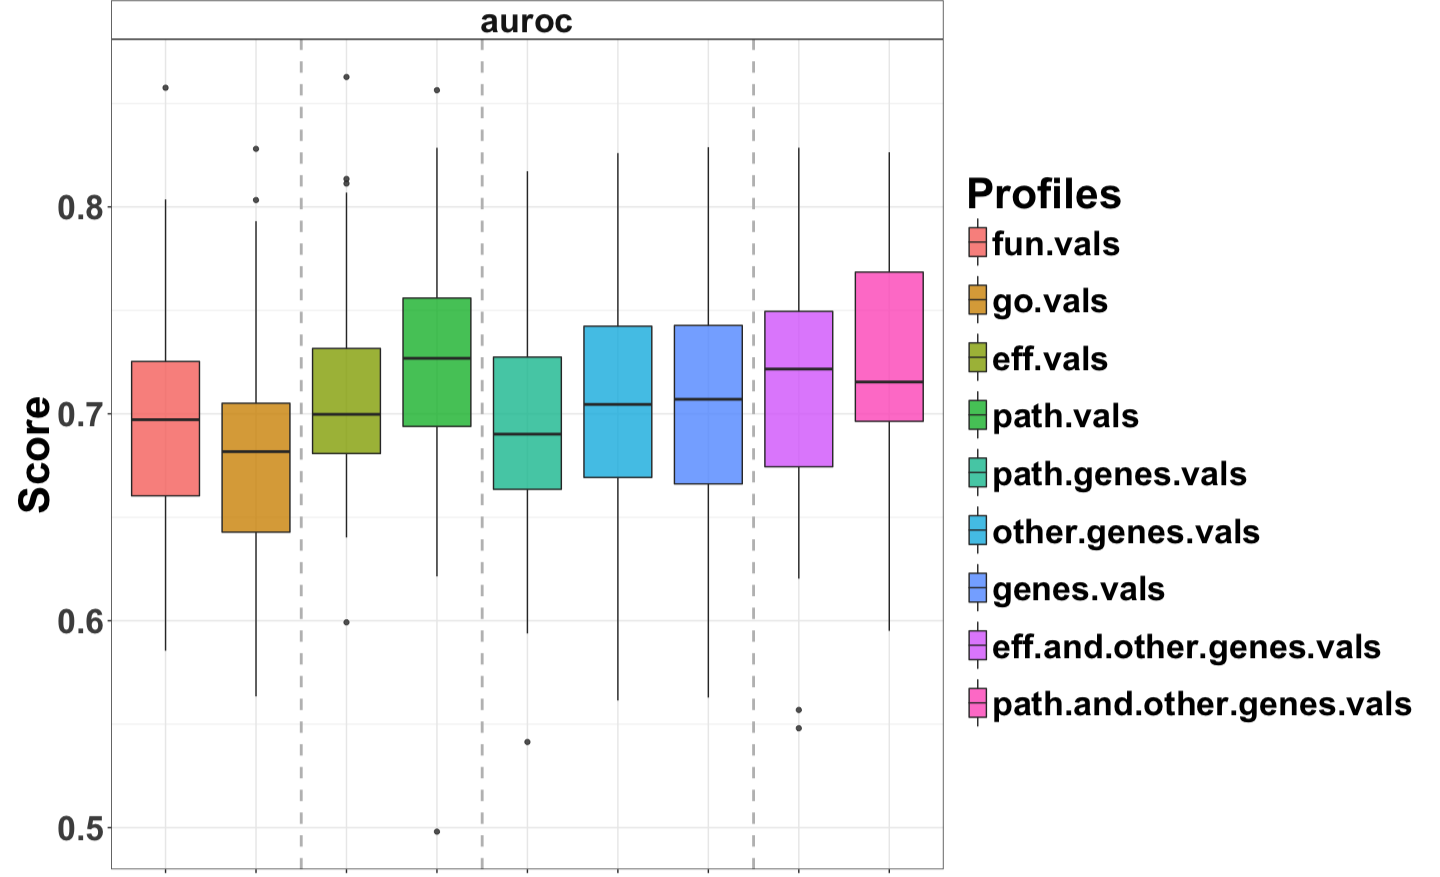
\includegraphics[width=0.8\textwidth]{ch-hipathia/results/score}
	\caption{The AUROC performance of using different types of profiles as predictive features to classify survival outcome for breast cancer patients. Boxplot represents the variance of the performance on 50 cross-validation splits. Dotted vertical lines separate profiles by the underlying analysis levels.}
	\label{fig4:score}
\end{figure}

\begin{table}[!htbp]
	\centering
	\caption{Mean AUROC scores with standard deviation (SD) and the top 2 most frequently selected classifiers by internal cross-validation for each type of prognostic profile in classifying breast cancer prognosis.}
	\begin{tabular}{|l|r|r|l|l|}
		\hline
		\textbf{Profile alias} & \textbf{Mean} & \textbf{SD} & \textbf{Classifier 1} & \textbf{Classifier 2} \\\hline
		\textit{fun.vals} & 0.6962 & 0.05438 & \textit{RadialSVM} & \textit{GBM} \\\hline
		\textit{go.vals} & 0.6807 & 0.06095 & \textit{RadialSVM} & \textit{LinearSVM} \\\hline
		\textit{eff.vals} & 0.7087 & 0.05099 & \textit{RadialSVM} & \textit{LinearSVM} \\\hline
		\textit{path.vals} & 0.7211 & 0.06316 & \textit{RadialSVM} & \textit{LinearSVM} \\\hline
		\textit{path.genes.vals} & 0.6938 & 0.05636 & \textit{RadialSVM} & \textit{LinearSVM} \\\hline
		\textit{other.genes.vals} & 0.7075 & 0.05254 & \textit{LinearSVM} & \textit{RadialSVM} \\\hline
		\textit{genes.vals} & 0.7075 & 0.05272 & \textit{LinearSVM} & \textit{RadialSVM} \\\hline
		\textit{eff.and.other.genes.vals} & 0.7127 & 0.05838 & \textit{LinearSVM} & \textit{RadialSVM} \\\hline
		\textit{path.and.other.genes.vals} & 0.7246 & 0.05359 & \textit{LinearSVM} & \textit{RadialSVM} \\\hline
	\end{tabular}
	\label{tab4:score}
\end{table}

\begin{sidewaystable}
	\centering
	\caption{FDR-adjusted p-values comparing the difference between the corresponding AUROC scores of profiles in columns and profiles in rows over 50 cross-validation splits. See Table \ref{tab4:score} for the mean scores of each profile individually. Significant p-values are boldfaced and marked with asterisks.}
	\renewcommand{\arraystretch}{1.3}
	\newcolumntype{R}{>{\raggedleft\arraybackslash}X}%
	\newcolumntype{L}{>{\raggedright\arraybackslash}X}%
	\begin{tabularx}{\textwidth}{|L|*{9}{R|}}
		\hline
		& \textit{go.vals} & \textit{eff.vals} & \textit{path.vals} & \textit{path.genes.-vals} & \textit{other.genes.-vals} & \textit{genes.vals} & \textit{eff.and.-other.-genes.vals} & \textit{path.and.-other.-genes.vals} \\\hline
		\textit{fun.vals} & 0.1467 & 0.1306 & \textbf{0.0119*} & 0.8267 & 0.1908 & 0.1908 & 0.0815 & \textbf{0.0020**} \\\hline
		\textit{go.vals} &  & \textbf{0.0024**} & \textbf{0.0004***} & 0.1557 & \textbf{0.0120*} & \textbf{0.0119*} & \textbf{0.0046**} & \textbf{$<$0.0001***} \\\hline
		\textit{eff.vals} &  &  & 0.0815 & \textbf{0.0255*} & 0.8743 & 0.8743 & 0.6422 & \textbf{0.0235*} \\\hline
		\textit{path.vals} &  &  &  & \textbf{0.0046**} & 0.1408 & 0.1394 & 0.3702 & 0.6422 \\\hline
		\textit{path.genes.-vals} &  &  &  &  & \textbf{0.0255*} & \textbf{0.0255*} & \textbf{0.0046**} & \textbf{0.0002***} \\\hline
		\textit{other.genes.-vals} &  &  &  &  &  & 0.9483 & 0.2167 & \textbf{0.0039**} \\\hline
		\textit{genes.vals} &  &  &  &  &  &  & 0.2000 & \textbf{0.0032**} \\\hline
		\textit{eff.and.-other.-genes.vals} &  &  &  &  &  &  &  & \textbf{0.0473*} \\\hline
	\end{tabularx}
	\label{tab4:test}
\end{sidewaystable}

When comparing the prognostic power between pathway-level and gene-level profiles, we have also derived cellular function activity profiles, denoted by \textit{fun.vals} and \textit{go.vals} (Table \ref{tab4:profile}), and observed that the performance of these profiles are slightly worse than other pathway-level profiles (Figure \ref{fig4:score}). This is probably due to the excessively simplistic procedure that basically averages the signaling activity values of effector circuits ending at proteins with the same annotated keywords according to UniProt or GO \cite{Hidalgo2017High}, annotations that can be incomplete and ambiguous to some extent.

Table \ref{tab4:score} summarizes the best-performing classifiers for each type of prognostic profile in the sense that they are most frequently selected by internal cross-validation. Notably, it evidences that Support Vector Machines with various kernels are recurrently selected as the competent classifier in breast cancer prognosis that suits well for both gene-level and pathway-level features.

\subsection{Signaling Circuits Selected as Features Relevant for Cancer Prognostic Account for Cancer Hallmarks}
\label{sec4:pathselect}

From the clinical standpoint of cancer prognosis, we are interested in identifying a small set of biomarkers that can guide decision making in cancer prognosis. As our analysis is made at the level of pathways, we would like to detect a few signaling circuits whose activity, and thus the underlying cell functionality, has a significant impact on discriminating the prognosis classes of cancer patients. We opted for the Random Forests classifier to perform this analysis, since it simultaneously predicts the survival outcome of tumor samples and scores the importance of each feature that is ultimately used in the prediction. We focus on the feature importance measure returned by fitting a Random Forest which accounts for the mean decrease in classification performance if we randomly permute the data of the corresponding feature.

Table \ref{tab4:path} lists the 5 top-scored circuits by fitting Random Forests with the profiles of circuit activities, denoted by \textit{path.vals}. The role played by each signaling circuit in cancer progression can be inferred from the underlying cellular functions (taken from GO annotations) triggered by the last (effector) protein on the circuit. Thus, the first circuit, belonging to the HIF-1 signaling pathway, starts with the TLR4 receptor, which is known to be related to progression of several cancers (breast, ovarian, prostate and head and neck) via lipopolysaccharide stimulation \cite{Yang2014Toll} and ends in the EDN1 effector, an hypoxia-inducible factor that mediates cancer progression \cite{Semenza2012Hypoxia}. Another relevant circuit belongs to the NF-kappa B signaling pathway and has the IL1B protein as receptor and the CXCL2 as effector. Polymorphisms in the receptor have been linked to several cancers in different populations \cite{El-Omar2000Interleukin, Lu2005Genetic} and it has been demonstrated the role of CXCL2 in tumor growth and angiogenesis \cite{Keane2004Depletion}. Similarly, polymorphisms in the LEP protein, the receptor of another circuit in the Adipocytokine signaling pathway, have been linked to cancer \cite{Cleveland2010Common}, and its effector, the tyrosine phosphatase Shp2 (PTPN11), contributes to the pathogenesis of many cancers and other human diseases \cite{Chan2008tyrosine}. The Cell cycle signaling pathway contains another relevant circuit whose receptor TTK transmits the signal until the cohesin complex. This four proteins complex is essential for chromosome segregation and DNA repair and mutations in its component genes have recently been identified in several types of tumors \cite{Losada2014Cohesin}. Finally, the last relevant circuit, belonging to the Tight junction pathway, contains the AKT3 serine/threonine kinase with a known role in tumorigenesis \cite{Testa2001AKT}, is signaled by the receptor ACTN4, a protein which has been related to cell invasion and metastasis \cite{Honda2015biological}. An expanded list of top-scored 50 circuits can be found in online supplementaries.

\begin{table}[!htbp]
	\centering
	\caption{Top 5 circuits with the highest feature importance measure by fitting Random Forests with \textit{path.vals} in classifying breast cancer prognosis, along their functions as annotated in Gene Ontology (GO).}
	\begin{tabularx}{\textwidth}{|l|X|X|X|X|}
		\hline
		\textbf{Rank} & \textbf{Pathway name} & \textbf{Receptor genes} & \textbf{Effector genes} & \textbf{Effector protein GO function} \\\hline
		1 & HIF-1 signaling pathway & TLR4 & EDN1 & Growth/survival factor in cancer \\\hline
		2 & NF-kappa B signaling pathway & IL1B & CXCL2 & Inflammatory response and angiogenesis \\\hline
		3 & Adipocytokine signaling pathway & LEP & PTPN11 & Protein phosphatase \\\hline
		4 & Cell cycle & TTK & Cohesin complex (SMC1B, SMC3, STAG1, RAD21) & Chromosome segregation and DNA repair \\\hline
		5 & Tight junction & ACTN4, MAGI3 & AKT3 & Cell invasion and metastasis \\\hline
	\end{tabularx}
	\label{tab4:path}
\end{table}

Table \ref{tab4:eff} lists the 5 top-scored effector circuits by fitting Random Forests with the profiles of effector circuit activities, denoted by \textit{eff.vals}. Although the cohesion complex effector is again selected, the effector circuit level analysis provided a slightly different perspective of relevant aspects of signaling in cancer patient survival. Thus, two effector circuits with effector proteins LEPR and PPAR$\alpha$, from the AMPK and the Adipocytokine signaling pathways, respectively, are activators of the fatty acid metabolism. Two more effector pathways ending in the Interleukin 6 (IL6), related to inflammatory processes and immune response in the Toll-like receptor pathway, seem more likely to be involved in blocking the cell differentiation through the Pathways in cancer (KEGG ID hsa05200). Actually, it has been described that IL6 blocks apoptosis in cells during the inflammatory process, keeping them alive in toxic environments, but the same process protects cells from apoptosis and chemotherapeutic drugs during neoplastic growth \cite{Hodge2005role}. An expanded list of top-scored 50 effector circuits can be found in the online supplementaries.

\begin{table}[!htbp]
	\centering
	\caption{Top 5 effector circuits with the highest feature importance measure by fitting Random Forests with \textit{eff.vals} in classifying breast cancer prognosis, along their functions as annotated in Gene Ontology (GO).}
	\begin{tabularx}{0.9\textwidth}{|l|X|X|X|}
		\hline
		\textbf{Rank} & \textbf{Pathway name} & \textbf{Effector genes} & \textbf{Effector protein GO function} \\\hline
		1 & AMPK signaling pathway & LEPR & Regulation of fatty acid metabolism \\\hline
		2 & Adipocytokine signaling pathway & PPAR$\alpha$ & Peroxisome proliferation and fatty acid metabolism \\\hline
		3 & Pathways in cancer & IL6 & Blockage of differentiation, Anti-apoptosis \\\hline
		4 & Cell cycle & Cohesin complex (SMC1B, SMC3, STAG1, RAD21) & Chromosome segregation and DNA repair \\\hline
		5 & Toll-like receptor signaling pathway & IL6 & Inflamation, Immune response, Anti-apoptosis \\\hline
	\end{tabularx}
	\label{tab4:eff}
\end{table}

\subsection{The Classification Algorithm Suggests Additional Prognostic Genes That Do Not Code for Signaling Proteins}
\label{sec4:othergene}

In order to find genes that could be relevant for patient survival that are not in the signal pathways, we have constructed a profile by combining signaling circuit activity profiles and gene expression profiles corresponding to other-genes absent from signaling pathways, denoted by \textit{path.and.other.genes.vals}. A feature selection procedure in breast cancer prognosis based on such a profile can select signaling circuits along with genes whose activity is unrelated to cell signaling but nonetheless related to patient survival. To this end, Random Forests was again used to score feature importance when fitted with the \textit{path.and.other.genes.vals} profile in the classification of breast cancer survival outcome.

Table \ref{tab4:othergene} lists the 5 top-scored other-genes that are part of the \textit{path.and.other.genes.vals} composed profile. These genes are of particular interest given that they might represent relevant cancer processes not included in cell signaling. Notably, the gene ABCB5 belongs to the ATP-binding cassette subfamily B which is well known to be involved in multiple drug resistance in cancer therapy \cite{Dean2001human}, probably due to its functionality of efflux transmembrane transporter. It has also been reported that ABCB5 could mediate cell-to-cell fusion and contribute to breast cancer chemoresistance in expressing breast tumors \cite{Frank2003Regulation, Frank2005ABCB5}. In addition, ABCB5, as a ``pro-survival'' gene, has been suggested to be a potential target against drug resistant breast cancer cells \cite{Yang2010p}. Besides, ABCB5 has been linked to melanoma \cite{Wilson2014ABCB5}. LMO4 encodes a LIM-domain protein that has been reported as an essential mediator of cell cycle progression in ErbB2/HER2/Neu-induced breast cancer which is characterized by poor survival due to high proliferation and metastasis rates \cite{Montanez-Wiscovich2009LMO4, Matthews2013LIM}. It has been reported that LMO4 interacts with the renowned tumor suppressor BRCA1 and inhibits BRCA1 activity \cite{Sum2002LIM, Sutherland2003Mutational}. OPA1 encodes a mitochondrial fusion protein which might be a target for mitochondrial apoptotic effectors \cite{Olichon2003Loss}, such as sorafenib \cite{Zhao2013OPA1}. The role in cancer survival played by two most important genes according to the results, VPS72 and CHADL, is not as clear from the literature. It is worth mentioning that a mutation in VPS72 in cervix cancer with a high FATHMM pathogenicity score \cite{Shihab2015integrative} is described in the COSMIC database (entry COSM458603). Regarding CHADL, it has been related to chondrocyte differentiation \cite{Tillgren2015novel} and extracellular matrix remodeling \cite{Barallobre-Barreiro2012Proteomics}. Therefore, both genes are potentially involved in cancer processes, which suggest that further investigation of the complete list of top-ranked other-genes could render new cancer drivers and potential therapeutic targets. An expanded list containing the top 50 most important features among the other-genes can be found in online supplementaries, in which many genes with cancer-related functions\footnote{Functions for those genes were taken from their UniProt annotations and, when absent, from GeneCards annotations \cite{Stelzer2016genecards}.} can be seen.

\begin{table}[!htbp]
	\centering
	\caption{Top 5 other-genes (genes unrelated to cell signaling) with the highest feature importance measure by fitting Random Forests with \textit{path.and.other.genes.vals} in classifying breast cancer prognosis, along their functions as annotated in Gene Ontology (GO).}
	\begin{tabularx}{\textwidth}{|l|l|l|X|X|}
		\hline
		\textbf{Rank} & \textbf{Gene ID} & \textbf{Gene symbol} & \textbf{Full name} & \textbf{GO function} \\\hline
		1 & 6944 & VPS72 & Vacuolar protein sorting 72 homolog & DNA binding \\\hline
		2 & 150356 & CHADL & Chondroadherin like & Collagen binding \\\hline
		3 & 340273 & ABCB5 & ATP binding cassette subfamily B member 5 & ATP binding, Efflux transmembrane transporter activity \\\hline
		4 & 8543 & LMO4 & LIM domain only 4 & Transcription factor activity, Sequence-specific DNA binding \\\hline
		5 & 4976 & OPA1 & OPA1, mitochondrial dynamin like GTPase & GTPase activity \\\hline
	\end{tabularx}
	\label{tab4:othergene}
\end{table}

\section{Discussion}
\label{sec4:discussion}

In this study we have proposed a novel scheme to classify survival outcome for breast cancer patients based on mechanistic features consisting of signaling pathway activity profiles. We applied a pathway activity analysis method \textit{hiPathia} \cite{Hidalgo2017High} to recode gene expression profiles into activity values of signaling circuits, and demonstrated that, making use of the state-of-the-art computational tools, signaling circuit activity yields better prediction in breast cancer prognosis than gene expression. An additional advantage is that the identified pathway-level biomarkers are mechanistic signatures whose contribution to cancer progression can be readily interpreted in terms of the underlying cellular functions and biological processes.

The three feature sets \textit{path.genes.vals}, \textit{eff.vals} and \textit{path.vals} are composed by the same set of genes, path-genes that are present in the pathways. However, pathway activity values recoded from these genes with the \textit{hiPathia} method, \textit{eff.vals} and \textit{path.vals}, clearly outperforms (see Table \ref{tab4:test}) the original path-genes, \textit{path.genes.vals}, in terms of prediction performance. Moreover, compared to the prediction performance with features based on all the genes, \textit{genes.vals}, that indeed carry more information than the subset of path-genes, features based on path-genes, \textit{path.genes.vals}, are significantly worse while features based on circuits of path-genes, \textit{eff.vals} and \textit{path.vals}, are competitive (see Table \ref{tab4:test}). It is worth noting that genes in the circuits assume only 12\% of the total number of genes. Therefore, it suggests that combining the genes into circuits provides a real added value for prediction purposes.

Although a significant improvement of the performance was not observed when the expression values of other-genes were concatenated to the activity values of signaling circuits, the analysis based on the combination of the two provides an interesting perspective regarding the interpretation of the biomarkers detected. In fact, the selected genes from the category of other-genes represent other aspects of the mechanism of the disease not explained by cell signaling. This approach allows expanding the scope of the analysis beyond the processes included in the pathways modeled.

Central to this study is the idea of promoting gene-level analysis to pathway-level analysis by obtaining personalized profiles of signaling circuit activity by applying the \textit{hiPathia} method. We deem that reliable models of pathway activity have the potential be used to derive robust multigenic biomarkers, in the spirit of renowned MammaPrint \cite{Veer2008Enabling}, which in addition account properly for the underlying disease mechanisms or mechanisms of drug action.


\cleardoublepage

\chapter{Conclusion and Future Work}
\label{chap:conclusion}

Thesis contributions:

- Theory

- Methodology

- Software

Research perspectives:

- machine learning

* theoretical guarantees on rankings
* constitutes an elegant confirmation of the concept of using ranking-related methods for bioinformatics but more ideas to motivate by social choice theory etc
* other cross-subject directions of future research such as pure math (geometric group theory, algebraic group theory, etc) and other biomedical application

- bioinformatics

* far from clinical... In fact, a voluminous literature of $>$150,000 papers documenting thousands of claimed biomarkers has been produced in medicine, of which fewer than 100 have been validated for routine clinical practice \cite{Poste2011Bring}. The very few number of gene expression-based breast cancer prognostic predictors successfully implemented in clinics compared to the number of research findings in this area raises controversies on the practical validity of molecular signatures. issues include: a large number of identified signatures failed to add significantly incremental values to assist prognosis assessment and therapeutic decision making upon the use of conventional clinical covariates; lack of proper validation and clinical utility; cost-effectiveness; etc \cite{Michiels2016Statistical}.
* opportunities come with caveats... overfitting or overly exaggeration of trivial findings... random genes associated to prognosis \cite{Venet2011Most}
* subtyping of breast cancers and prognosis/treatment for each subtype
* integrative data analysis, multi-view multi-omics analysis, incorporating with clinical variables (quote Sage-DREAM BCC)
* meta-analysis with multiple datasets or cross-study validation
* pan-cancer - attractor metagenes
* wet-lab experimental validation
* section 6.3.6 of JP book pitfalls in biomarker discovery

Our knowledge towards cancer biology is still far from complete but we are given the extraordinary opportunity in the era of big data to study cancer.

% ch2-3 embedding for permutations ?!
% other embedding - just (1,\dots,n) or permutation matrix - high-order embedding
% what is the convex hull of Kendall embedding for
%Check Fogel (NIPS, 2013) and Stephen Wright (NIPS, 2014) for two embeddings of symmetric group $\mathbb{S}_n$ into Euclidean spaces, former into dim $n^2$ while latter into dim $n-1$ (or a hyperplane in dim $n$), thus facilitating the convex relaxation to seriation problems by solving an optimization problem constrained in a convex hull, former in Birkhoff polytope
%$$\mathcal{B}:=\{\mathbf{X}\in \mathbb{R}^{n\times n}:\mathbf{X}\succeq 0,\mathbf{X}\mathbf{1}=\mathbf{1},\mathbf{X}^T \mathbf{1}=\mathbf{1}\}$$
%while latter in permutahedron
%$$\mathcal{PH}:=\{x\in \mathbb{R}^n:\sum_{i=1}^n x_i=\frac{n(n+1)}{2},\sum_{i\in S}x_i \leq \sum_{i=1}^{|S|}(n+1-i)\mbox{ for all }S\subset [n]\}.$$
%Kendall kernel comes with another embedding into Euclidean space of dim $O(n^2)$. Several questions are
%\begin{enumerate}
%\item What is the convex hull induced by our embedding? What is the projection of any vector onto the convex hull (to facilitate optimization algorithm using projections)?
%\item On the other way round, what are the explicit embedding, kernel function and distance induced by those two well-known embeddings?
%\item Is it a better embedding compared to those two embeddings to introduce a convex hull for solving seriation problem, when we convert it into an optimization problem by following the same idea as Fogel (NIPS, 2013) after the embedding?
%\end{enumerate}


\cleardoublepage

% appendix
\appendix
\chapter{A Tractable Bound on Approximating Kemeny Aggregation}
\label{chap:kemeny}

\begin{chapabstract}

\textrm{{\bf Abstract:}} Due to its numerous applications, rank aggregation has become a problem of major interest across many fields of the computer science literature. In the vast majority of situations, Kemeny consensus is considered as the ``golden'' solution. It is however well known that its computation is NP-hard. Much contribution have thus been devoted to establishing various results to apprehend this complexity. In this chapter, we introduce a practical method to predict, given a dataset and a ranking typically output by some approximate procedure, how close this ranking is to the Kemeny consensus of the dataset. A major strength of the proposed method is its generality: it requires little assumption on the dataset nor the ranking. Furthermore, it relies on a geometric interpretation of Kemeny aggregation that we believe could paves way to other results beyond those presented in this chapter. This study has been published as joint work with Anna Korba and Eric Sibony \cite{Jiao2016Controlling}.
\linebreak
\vskip 0.1in
\noindent \textrm{{\bf R�sum�:}}

\end{chapabstract}

\section{Introduction}

Given a collection of rankings on a set of alternatives, how to aggregate them into one ranking? This rank aggregation problem has gained a major interest across many research fields. Starting from elections in social choice theory \cite{Borda1781Memoire, Condorcet1785Essai, Arrow1950difficulty, Xia2015Generalized}, it has been applied to meta-search engines \cite{Dwork2001Rank, Renda2003Web, Desarkar2016Preference}, competitions ranking \cite{Davenport2005Ranking, Deng2014Bayesian}, analysis of biological data \cite{Kolde2012Robust, Patel2013Hierarchical} or natural language processing \cite{Li2014Learning, Zamani2014Regression} among others.

Among many ways of formulating the problem of rank aggregation stands out the Kemeny aggregation \cite{Kemeny1959Mathematics}. Defined as the problem of minimizing a cost function over the symmetric group (see Section \ref{secA:problem-statement} for definition), its solutions, called Kemeny consensuses, have been shown to satisfy desirable properties from many points of view \cite{Young1978consistent}.

Computing a Kemeny consensus is however NP-hard, even for only four rankings \cite{Bartholdi1989computational, Cohen1999Learning, Dwork2001Rank}. This fact has motivated the research community to introduce many approximate procedures and to evaluate them on datasets (see, for instance, \cite{Schalekamp2009Rank, Ali2012Experiments}). It has also triggered a tremendous amount of work of obtaining theoretical guarantees on these procedures and more generally in understanding the complexity of Kemeny aggregation from various perspectives. Some have proven bounds on the approximation cost of the approximate procedures \cite{Diaconis1977Spearmans, Coppersmith2006Ordering, VanZuylen2007Deterministic, Ailon2008Aggregating, Freund2015Rank}, while some have established recovery properties \cite{Saari2000geometric, Procaccia2012Maximum}. Notably it has been shown that exact Kemeny aggregation is tractable if some quantity is known on the dataset \cite{Betzler2008Fixed, Betzler2009How, Cornaz2013Kemeny} or if the dataset satisfies some conditions \cite{Brandt2015Bypassing}. Besides, some contributions have established approximation bounds that can be computed on the dataset \cite{Davenport2004computational, Conitzer2006Improved, Sibony2014Borda}.

In this chapter we introduce a novel approach to apprehend the complexity of Kemeny aggregation. Consider the following question: \textit{Given a dataset and a ranking typically output by some approximate procedure, can we predict how close the ranking is to any Kemeny consensus without computing the latter?} We exhibit a tractable quantity that allows to give a positive answer to this question. The main contribution of our results is a simple and practical method to obtain such a guarantee for the outcome of an aggregation procedure on any dataset. A major strength of our approach is its generality: it applies to all aggregation procedures and to any dataset. Further, our results are based on a geometric analysis of Kemeny aggregation (see Section \ref{secA:geometry}) that has been unprecedentedly exploited in the literature yet but constitutes a powerful tool. We thus take efforts to explain it in details. We believe that it could pave way to many other results on Kemeny aggregation beyond those presented here.

The chapter is structured as follows. Section \ref{secA:problem-statement} introduces the general notations and states the question of interest. The geometric analysis is detailed in Section \ref{secA:geometry} and further studied in Section \ref{secA:proof} while our main result is presented in Section \ref{secA:main-result}. Finally, numerical experiments are reported in Section \ref{secA:experiments} to address the efficacy and usefulness of our method on datasets from real-world applications.



\section{Kemeny Aggregation Problem}
\label{secA:problem-statement}


Let $\n = \cbr{1,\dots,n}$ be a set of alternatives to be ranked. In this study, we focus only on total rankings. A total ranking $a_1 \succ \dots \succ a_n$ on $\n$ is interchangeably seen as the permutation $\sigma$ of $\n$ that maps an item to its rank: $\sigma(a_i)=i$ for $i \in \n$. The set of all permutations of $\n$ is called the symmetric group and denoted by $\Sn$. Given a collection of $N$ permutations $\DN = \left(\sigma_{1},\dots,\sigma_{N}\right)\in\Sn^{N}$, Kemeny aggregation aims at solving
\begin{equation}
\label{eqA:Kemeny-aggregation}
\min_{\sigma\in\Sn} \sum_{t=1}^{N}d(\sigma,\sigma_{t}) \,,
\end{equation}
where $d$ is the Kendall's tau distance defined for $\sigma,\sigma' \in \Sn$ as the number of their pairwise disagreements: $d(\sigma,\sigma') = \sum_{1\leq i < j \leq n}\hollowone\{(\sigma(j)-\sigma(i))(\sigma'(j)-\sigma'(i))<0\}$. The objective function in \eqref{eqA:Kemeny-aggregation} denotes the cost, and a permutation $\sigstar$ solving \eqref{eqA:Kemeny-aggregation} is called a Kemeny consensus. We denote by $\KN$ the set of Kemeny consensuses on the dataset $\DN$.

Exact Kemeny aggregation is NP-hard: it cannot be solved efficiently with a general procedure. This does not mean however that nothing can be done. For example, it is clear that on a dataset where all permutations are equal to a $\sigma_{0}\in\Sn$, the Kemeny consensus is trivially given by $\sigma_{0}$. Many contributions from the literature have thus focused on particular approaches to apprehending some part of the complexity of Kemeny aggregation. The examples given in the introduction generally fall in three categories:
\begin{bulletList}
	\item \textbf{General guarantees for approximate procedures.} These results provide a bound on the cost of a specific voting rule, valid for any dataset \cite{Diaconis1977Spearmans, Coppersmith2006Ordering, VanZuylen2007Deterministic, Ailon2008Aggregating, Freund2015Rank}.
	\item \textbf{Bounds on the approximation cost computed from the dataset.} These results provide a bound, either on the cost of a consensus or on the cost of the outcome of a specific voting rule, that depends on a quantity computed from the dataset \cite{Davenport2004computational, Conitzer2006Improved, Sibony2014Borda}.
	\item \textbf{Conditions for the exact Kemeny aggregation to become tractable.} These results ensure the tractability of exact computation of Kemeny aggregation if the dataset satisfies some condition or if some quantity is known from the dataset \cite{Betzler2008Fixed, Betzler2009How, Cornaz2013Kemeny, Brandt2015Bypassing}.
\end{bulletList}
In this chapter, we introduce a novel approach, which falls into the second category above, to apprehend the complexity of Kemeny aggregation by considering the following question (henceforth referred to as The Question):

\begin{question*}
Let $\sigma\in\Sn$ be a permutation, typically output by a computationally efficient aggregation procedure on $\DN$. Can we use tractable quantities to give an upper bound on the distance $d(\sigma,\sigstar)$ between $\sigma$ and any Kemeny consensus $\sigstar$ on $\DN$?
\end{question*}


The answer to The Question is positive as we will elaborate in this study. We propose an upper bound, guaranteed by Theorem \ref{thmA:method}, thus says: for any $\sigma$ and $\DN$, we have $d(\sigma,\sigstar)\leq \kmin$ for all consensuses $\sigstar\in\KN$, where $\kmin$ is defined in \eqref{eqA:k-min}. We would like to stress a major strength of our method compared to those previously studied in literature that is the generality: it can be applied to any dataset $\DN$ and any permutation $\sigma$ with little assumption on neither. This is because it exploits a powerful geometric framework for the analysis of Kemeny aggregation.



\section{Geometric Analysis of Kemeny Aggregation}
\label{secA:geometry}

Because of its rich mathematical structure, Kemeny aggregation can be analyzed from many different point of views. For instance, some contributions deal directly with the combinatorics of the symmetric group \cite{Diaconis1977Spearmans, Blin2011Median}, some work on the pairwise comparison graph \cite{Coppersmith2006Ordering, Conitzer2006Improved, Jiang2011Statistical}, and some exploit the geometry of the Permutahedron \cite{Saari2000geometric}. In this chapter, we analyze it via the Kendall embedding \cite[Theorem 1]{Jiao2015Kendall}. For the self-containment of this chapter, recall from the proof of Theorem \ref{thm2:main} that we have used the following definition.\footnote{We will omit the scaling constant $\frac{1}{\binom{n}{2}}$ due to its irrelevance in this study and use $\phi$ instead of $\Phi$ to distinguish this trivial difference.}

\begin{definition}[Kendall embedding]
The Kendall embedding is the mapping $\phi : \Sn \rightarrow \RR^{\binom{n}{2}}$ defined by
\[
\phi:\sigma \mapsto 
\left(\begin{array}{c}
\vdots\\
\sgn(\sigma(i)-\sigma(j))\\
\vdots
\end{array}\right)_{1 \leq i < j \leq n} \,,
\]
where the sign function $\sgn(x) = 1$ if $x > 0$ and $-1$ if $x < 0$ and $0$ otherwise.
\end{definition}

The Kendall embedding $\phi$ maps a permutation to a vector in $\RR^{\binom{n}{2}}$ where each coordinate is indexed by an (unordered) pair $\{i,j\}\subset\n$ (we choose $i<j$ by convention). Though this vector representation is equivalent to representing a permutation as a flow on the complete graph on $\n$, it allows us to perform a geometric analysis of Kemeny aggregation in the Euclidean space $\RR^{\binom{n}{2}}$. Denoting by $\innerprod{\cdot,\cdot}$ the canonical inner product and $\nm{\cdot}$ the Euclidean norm, the starting point of our analysis is the following result, already brought up by \cite{Barthelemy1981median} and rephrased in the proof of Theorem \ref{thm2:main}.

\begin{proposition}[Background results]
\label{propA:background-result}
For all $\sigma,\sigma'\in\Sn$,
\[
\nm{\phi(\sigma)} = \sqrt{\frac{n(n-1)}{2}} := R \;\text{and}\; \nm{\phi(\sigma) - \phi(\sigma')}^2 = 4 d(\sigma,\sigma') \,,
\]
and for any dataset $\DN=(\sigma_{1},\dots\sigma_{N})\in\Sn^{N}$, Kemeny aggregation \eqref{eqA:Kemeny-aggregation} is equivalent to the minimization problem
\begin{equation}
\label{eqA:reformulation}
\min_{\sigma\in\Sn} C_{N}(\sigma) := \Vert\phi(\sigma)-\phi(\DN)\Vert^{2} \,,
\end{equation}
where
\begin{equation}
\label{eqA:mean-embedding}
\phi\br{\DN} := \frac{1}{N}\sum_{t=1}^{N}\phi\br{\sigma_t}.
\end{equation}
\end{proposition}

Proposition \ref{propA:background-result} leads to the following geometric point of view of Kemeny aggregation, illustrated by Figure \ref{figA:geometric-interpretation}. First, as $\nm{\phi(\sigma)} = \sqrt{n(n-1)/2}$ for all $\sigma\in\Sn$, the embeddings of all the permutations in $\Sn$ lie on a sphere centered at $0$ with radius $R = \sqrt{n(n-1)/2}$. Notice that $\nm{\phi(\sigma) - \phi(\sigma')}^2 = 4 d(\sigma,\sigma')$ for all $\sigma,\sigma'\in\Sn$ implies that $\phi$ is injective, in other words that it maps two different permutations to two different points on the sphere. A dataset $\DN = (\sigma_{1},\dots,\sigma_{N})\in\Sn^{N}$ is thus mapped to a weighted point cloud on this sphere, where for any $\sigma\in\Sn$, the weight of $\phi(\sigma)$ is the number of times $\sigma$ appears in $\DN$. The vector $\phi(\DN)$, defined by \eqref{eqA:mean-embedding}, is then equal to the barycenter of this weighted point cloud. We call it the \textit{mean embedding} of $\DN$. Now, the reformulation of Kemeny aggregation given by \eqref{eqA:reformulation} means that a Kemeny consensus is a permutation $\sigstar$ whose embedding $\phi(\sigstar)$ is closest to $\phi(\DN)$, \textit{with respect} to the Euclidean norm in $\RR^{\binom{n}{2}}$.

\begin{figure}[!htbp]
	\begin{center} 
		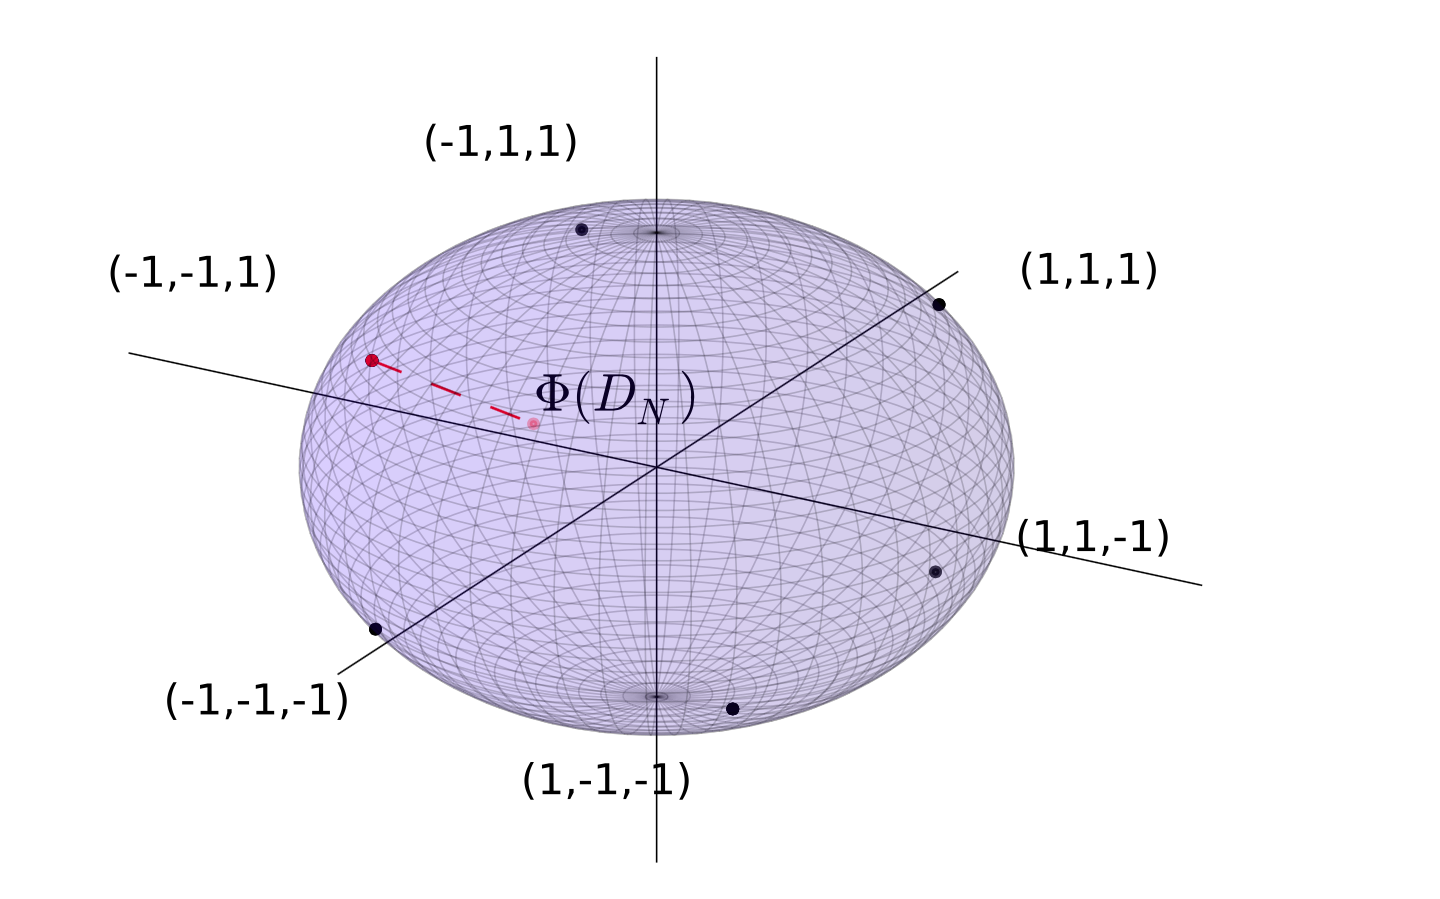
\includegraphics[trim=2cm 2cm 3cm 2cm, clip=true, width=0.6\textwidth, height=2.5in]{ch-kemeny/figures/3d1test}
	\end{center}
	\caption{Kemeny aggregation for $n=3$.}
	\label{figA:geometric-interpretation}
\end{figure}


From an algorithmic point of view, Proposition \ref{propA:background-result} naturally decomposes problem \eqref{eqA:Kemeny-aggregation} of Kemeny aggregation in two steps: first compute the mean embedding $\phi(\DN)$ in the space $\RR^{\binom{n}{2}}$, and then find a consensus $\sigstar$ as a solution of problem \eqref{eqA:reformulation}. The first step is naturally performed in $O(Nn^{2})$ operations. The NP-hardness of Kemeny aggregation thus stems from the second step. In this regard, one may argue that having $\phi(\DN)$ does not greatly alleviate the complexity in identifying an exact Kemeny consensus. However, a closer look at the problem leads us to asserting that $\phi(\DN)$ contains rich information about the location of the Kemeny consensuses. More specifically, we show in Theorem \ref{thmA:method} that the knowledge of $\phi(\DN)$ helps to provide an upper bound for the distance between a given permutation $\sigma\in\Sn$ and any Kemeny consensus $\sigstar$.


In fact, Proposition \ref{propA:background-result} implies that Kemeny's rule is a ``Mean Proximity Rule'', a family of voting rules introduced in \cite{Zwicker2008Consistency} and further studied in \cite{Lahaie2014Neutrality}. Our approach actually applies more generally to other voting rules from this class but we focus our discussion on Kemeny's rule in this study for the sake of clarity.


\section{Controlling the Distance to Kemeny Consensus}
\label{secA:main-result}

In this section, we now state our main results and demonstrate with an illustrative example how our proposed method addresses The Question. For a permutation $\sigma\in\Sn$, let us define the angle $\theta_{N}(\sigma)$ between $\phi(\sigma)$ and $\phi(\DN)$ by 
\begin{equation}
\label{eqA:cosinus}
\cos(\theta_{N}(\sigma)) = \frac{\innerprod{\phi(\sigma),\phi(\DN)}}{{\nm{\phi(\sigma)}\nm{\phi(\DN)}}},
\end{equation}
with $0 \leq \theta_{N}(\sigma)\leq \pi$ by convention.

\begin{thm}
\label{thmA:method}
Let $\DN\in\Sn^N$ be a dataset and $\sigma\in\Sn$ a permutation. For any integer $0 \leq k \leq \binom{n}{2}-1$, one has the following implication:
\[
\cos(\theta_{N}(\sigma)) > \sqrt{1-\frac{k+1}{\binom{n}{2}}}\quad\Longrightarrow\quad \max_{\sigstar\in\KN}d(\sigma,\sigstar) \leq k.
\]
\end{thm}

The proof of Theorem \ref{thmA:method} along with its geometric interpretation are postponed to Section \ref{secA:proof}. Broadly speaking, Theorem \ref{thmA:method} ensures that if the angle $\theta_{N}(\sigma)$ between the embedding $\phi(\sigma)$ of a permutation $\sigma\in\Sn$ and the mean embedding $\phi(\DN)$ is small, then the Kemeny consensuses cannot be too far from $\sigma$. Its application in practice is straightforward. Assume that one applies an aggregation procedure on $\DN$ (say the Borda Count for instance) that outputs $\sigma$. A natural question is then: how far is it from the Kemeny consensuses in terms of Kendall's tau distance? It is well known that the Kendall's tau distance takes values in $\{0,\dots,\binom{n}{2}\}$ \cite{Stanley1986Enumerative}. Consequently, the distance is at most equal to $\max_{\sigma',\sigma''\in\Sn} d(\sigma',\sigma'') = \binom{n}{2}$. But if one computes the quantity $\cos(\theta_{N}(\sigma))$, a better bound can be allowed due to Theorem \ref{thmA:method}. More specifically, the best bound is given by the minimal $k\in\{0,\dots,\binom{n}{2}-1\}$ such that $\cos(\theta_{N}(\sigma)) > \sqrt{1-(k+1)/\binom{n}{2}}$. Denoting by $\kmin(\sigma;\DN)$ this integer, it is easy to see that
\begin{equation}
\label{eqA:k-min}
\kmin(\sigma;\DN) = 
\left\{
\begin{array}{ll}
\left\lfloor \binom{n}{2}\sin^{2}(\theta_{N}(\sigma))\right\rfloor & \text{if } 0 \leq \theta_{N}(\sigma) \leq \frac{\pi}{2}\\
\binom{n}{2} & \text{if } \frac{\pi}{2} \leq \theta_{N}(\sigma) \leq \pi.
\end{array}
\right.
\end{equation}
where $\lfloor x\rfloor$ denotes the integer part of the real $x$. We formalize this method (henceforth referred to as The Method) in the following description.

\begin{method*}
Let $\DN\in\Sn^{N}$ be a dataset and let $\sigma\in\Sn$ be a permutation considered as an approximation of Kemeny's rule. In practice $\sigma$ is the consensus returned by a tractable voting rule. Then by Theorem \ref{thmA:method}, we have $d(\sigma,\sigstar) \leq \kmin(\sigma;\DN)$ for any Kemeny consenus $\sigstar\in\KN$, where $\kmin(\sigma;\DN)$ is obtained by \eqref{eqA:k-min}.
\end{method*}

The following proposition ensures that The Method has tractable complexity.

\begin{proposition}[Complexity of The Method]
The application of The Method has complexity in time $O(Nn^{2})$.
\end{proposition}

With a concrete example, we demonstrate the applicability and the generality of The Method.

\begin{example}[Application of The Method to the sushi dataset]
We report here the results of a case-study on the sushi dataset provided by \cite{Kamishima2003Nantonac} to illustrate our method. The dataset consists of $N=5000$ total rankings given by different individuals of the preference order on $n=10$ sushi dishes such that a brute-force search for the Kemeny consensus is already very computationally intensive. To apply our method, we selected seven tractable voting rules, denoted by $\sigma$, as approximate candidates to Kemeny's rule to provide an initial guess (details of voting rules can be found in Section \ref{secA:votingrules}). Table \ref{tabA:sushi} summarizes the values of $\cos(\theta_N(\sigma))$ and $\kmin(\sigma)$, respectively given by \eqref{eqA:cosinus} and \eqref{eqA:k-min}. Results show that on this particular dataset, if we use for instance Borda Count to approximate a Kemeny consensus, we are confident that any exact consensus has a distance of at most 14 to the approximate ranking. We detail empirical analysis of the results further in Section \ref{secA:experiments}.
\end{example}

\begin{table}[!htbp]
	\caption{Summary of a case-study on the applicability of The Method with the sushi dataset $(N=5000,n=10)$. Rows are ordered by increasing $\kmin$ (or decreasing cosine) value.}
	\label{tabA:sushi}
	\begin{center}
		\begin{tabular}{c|c|c}
			\hline
			Voting rule & $\cos(\theta_N(\sigma))$ & $\kmin(\sigma)$ \\
			\hline
			Borda & 0.820 & 14 \\
			Copeland & 0.822 & 14 \\
			QuickSort & 0.822 & 14 \\
			Plackett-Luce & 0.80 & 15 \\
			2-approval & 0.745 & 20 \\
			1-approval & 0.710 & 22 \\
			Pick-a-Perm & 0.383$^\dag$ & 34.85$^\dag$ \\
			Pick-a-Random & 0.377$^\dag$ & 35.09$^\dag$ \\
			\hline		
		\end{tabular}
	\end{center}
	\rule{0in}{1.2em}$^\dag$\scriptsize  For randomized methods such as Pick-a-Perm and Pick-a-Random, results are averaged over 10,000 computations.
\end{table}



\section{Geometric Interpretation Revisit and Proof of Theorem \ref{thmA:method}}
\label{secA:proof}

This section details the proof of Theorem \ref{thmA:method} based the geometric interpretation introduced in Section \ref{secA:geometry}. We deem that our proof has indeed a standalone interest, and that it could pave way to other profound results on Kemeny aggregation.

\subsection{Extended Cost Function}

Recall that the Kemeny consensuses of a dataset $\DN$ are the solutions of the problem \eqref{eqA:reformulation}:
\[
\min_{\sigma\in\Sn}C_{N}(\sigma) = \nm{\phi(\sigma)-\phi(\DN)}^{2} \,.
\]
This is an optimization problem on the discrete set $\Sn$, naturally hard to analyze. In particular the shape of the cost function $C_{N}$ is not easy to understand. However, since all the vectors $\phi(\sigma)$ for $\sigma\in\Sn$ lie on the sphere
\[
\Sphere := \left\{ x \in \RR^{\binom{n}{2}} \vert \nm{x} = R \right\} \,,
\]
where radius $R$ is the equal norm of the embedded point of any permutation and by Proposition \ref{propA:background-result},
\[
R = \sqrt{\frac{n(n-1)}{2}} \,.
\]
It is natural to consider the relaxed problem on $\Sphere$ that reads
\[
\min_{x\in\Sphere}\CN(x):=\nm{x-\phi(\DN)}^{2} \,.
\]
We call $\CN$ the extended cost function with domain $\Sphere$. The advantage of $\CN$ is that it has a very simple shape. We denote by $\theta_{N}(x)$ the angle between a vector $x\in\Sphere$ and $\phi(\DN)$ (with the slight abuse of notations that $\theta_{N}(\phi(\sigma)) \equiv \theta_{N}(\sigma)$). For any $x\in\Sphere$, one has
\[
\CN(x) = R^{2}+\nm{\phi(\DN)}^{2} - 2R\nm{\phi(\DN)}\cos(\theta_{N}(x)) \,.
\]
This means that the extended cost $\CN(x)$ of a vector $x\in\Sphere$ only depends on the angle $\theta_{N}(x)$. The level sets of $\CN$ are thus of the form $\{x\in\Sphere \;\vert\; \theta_{N}(x) = \alpha \}$, for $0\leq \alpha \leq \pi$. If $n=3$, these level sets are circles in planes orthogonal to $\phi(\DN)$, each centered around the projection of the latter on the plane (Figure \ref{figA:level-sets}). This property implies the following result.

\begin{lemma}
\label{lemA:angles}
A Kemeny consensus of a dataset $\DN$ is a permutation $\sigstar$ such that:
\[
\theta_{N}(\sigstar) \leq \theta_{N}(\sigma) \qquad\text{for all }\sigma\in\Sn \,.
\]
\end{lemma}

Lemma \ref{lemA:angles} means that the problem of Kemeny aggregation translates into finding permutations $\sigstar$ that have minimal angle $\theta_{N}(\sigstar)$. This reformulation is crucial to our approach.

\begin{figure}[!htbp]
	\begin{center}
		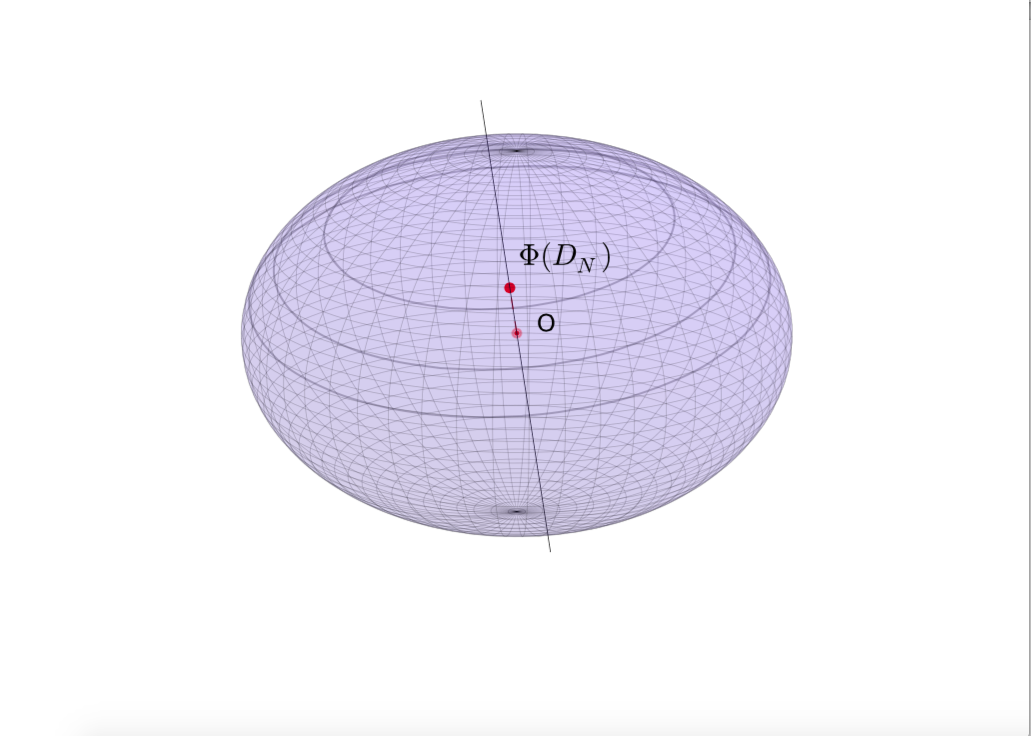
\includegraphics[trim=2cm 6cm 1cm 4cm, clip=true,  width=0.6\textwidth, height=2in]{ch-kemeny/figures/3d2test}
	\end{center}
	\caption{Level sets of the extended cost function $\CN$ over $\Sphere$ for $n=3$.}
	\label{figA:level-sets}
\end{figure}

\subsection{Interpretation of the Condition in Theorem \ref{thmA:method}}

The second element of our approach is motivated by the following observation. Let $x\in\Sphere$ be a point on the sphere and let $r \geq 0$. If $r$ is large enough, then all the points $x'\in\Sphere$ on the sphere that have distance $\nm{x'-x}$ greater than $r$ will have a greater angle $\theta_{N}(x')$. Formally, we denote by $\mathcal{B}(x,r) = \{x'\in\RR^{\binom{n}{2}} \;\vert\; \nm{x'-x} < r\}$ the (open) ball of center $x$ and radius $r$. Then one has the following result.

\begin{lemma}
\label{lemA:condition}
For $x\in\Sphere$ and $r\geq 0$, one has the following implication:
\[
\cos(\theta_{N}(x)) > \sqrt{1 - \frac{r^{2}}{4R^{2}}} \; \Longrightarrow \min_{x'\in\Sphere\setminus \mathcal{B}(x,r)}\theta_{N}(x') > \theta_{N}(x) \,.
\]
\end{lemma}

\begin{proof}
Let $\bar{\phi}(\DN) = \frac{\phi(\DN)}{\nm{\phi(\DN)}}$. We discuss over two cases.

\noindent {\bf Case I:} $\nm{\bar{\phi}(\DN) - x} \geq r.$ By laws of cosines, this case is equivalent to:
\begin{multline*}
2 R^2 (1-\cos(\theta_N(x))) = \nm{\bar{\phi}(\DN)  - x}^2 \geq r^2  \\
\Longleftrightarrow \cos(\theta_N(x)) \leq 1-\frac{r^2}{2R^2} \leq 1 -\frac{r^2}{4R^2} \,.
\end{multline*}
Note also that in this case, we have $\bar{\phi}(\DN)  \in \Sphere\setminus \mathcal{B}(x,r)$ and hence $\min_{x'\in\Sphere\setminus \mathcal{B}(x,r)}\theta_{N}(x') = \min_{x'\in\Sphere}\theta_{N}(x') = 0 \leq \theta_N(x)$ always holds, where the minimum is attained at $x'=\bar{\phi}(\DN)$.

\noindent {\bf Case II:} $\Vert\bar{\phi}(\DN)  - x\Vert < r$, that is $\bar{\phi}(\DN)  \in \mathcal{B}(x,r)$. As the function $x'\mapsto\theta_{N}(x')$ is convex with global minimum in $\mathcal{B}(x,r)$, its minimum over $\Sphere\setminus \mathcal{B}(x,r)$ is attained at the boundary $\Sphere \cap \partial \mathcal{B}(x,r) = \{x'\in\RR^{{n \choose 2}} \;\vert\; \nm{x'} = R \text{ and } \nm{x'-x} = r \}$, which is formed by cutting $\Sphere$ with the $\br{{n \choose 2}-1}$-dimensional hyperplane written as
$$
\mathbb{L} := \Big\{ x'\in\RR^{{n \choose 2}}\;\Big\vert\;\innerprod{x',x} = \frac{2R^2-r^2}{2}\Big\} \,.
$$
Straightforwardly one can verify that $\Sphere \cap \partial \mathcal{B}(x,r)$ is in fact a $\br{{n \choose 2}-1}$-dimensional sphere lying in $\mathbb{L}$, centered at $c = \frac{2R^2-r^2}{2R^2} x$ with radius $\gamma = r \sqrt{1-\frac{r^2}{4R^2}} \,.$ Now we take effort to identify:
$$
x^* = \argmin_{x' \in \Sphere \cap \partial \mathcal{B}(x,r)} \theta_N(x') = \argmin_{x' \in \Sphere \cap \partial \mathcal{B}(x,r)} \CN(x') \,.
$$
Note that $\phi(\DN)$ projected onto $\mathbb{L}$ is the vector $(\phi(\DN))_{\mathbb{L}} := \phi(\DN) - \frac{\innerprod{\phi(\DN),x}}{R^2}x.$ One can easily verify by Pythagoras rule that, for any set $\mathbb{K}\subseteq\mathbb{L}$,
$$
\argmin_{x'\in\mathbb{K}} \nm{x'-\phi(\DN)} = \argmin_{x'\in\mathbb{K}} \nm{x'-(\phi(\DN))_\mathbb{L}} \,.
$$
Therefore we have:
\begin{multline*}
x^* = \argmin_{x' \in \Sphere \cap \partial \mathcal{B}(x,r)} \nm{x'-(\phi(\DN))_\mathbb{L}} = c + \gamma \frac{(\phi(\DN))_\mathbb{L}}{\nm{(\phi(\DN))_\mathbb{L}}} \\
= \frac{2R^2-r^2}{2R^2} x + r \sqrt{1-\frac{r^2}{4R^2}} \frac{\phi(\DN) - \frac{\innerprod{\phi(\DN),x}}{R^2}x}{\sqrt{\nm{\phi(\DN)}^2 - \frac{\innerprod{\phi(\DN),x}^2}{R^2}}}\,.
\end{multline*}
Tedious but undemanding calculation leads to
\begin{equation*}
\theta_{N}(x^*) > \theta_{N}(x) \Longleftrightarrow \innerprod{x^*, \phi(\DN)} > \innerprod{x, \phi(\DN)} \Longleftrightarrow \cos(\theta_{N}(x)) > \sqrt{1 - \frac{r^{2}}{4R^{2}}} \,.
\end{equation*}
\end{proof}

It is interesting to look at the geometric interpretation of Lemma \ref{lemA:condition}. In fact, it is clear from the proof that $x^*$ should lie in the 2-dimensional subspace spanned by $\phi(\DN)$ and $x$. We are thus able to properly define multiples of an angle by summation of angles on such linear space $2\theta_N(x) := \theta_N(x) + \theta_N(x)$. Figure \ref{figA:illustration-condition} provides an illustration of Lemma \ref{lemA:condition} in this 2-dimensional subspace from the geometric point of view. In words, provided that $\theta_N(x)\leq \pi/2$, $x^*$ has a smaller angle than $x$ is equivalently written using laws of cosines as
\begin{multline*}
r^2 = \nm{x - x^*}^2 > 2 R^2 \big(1-\cos(2\theta_N(x))\big) \\
\Longleftrightarrow \cos(2\theta_N(x)) > 1 - \frac{r^2}{2R^2}
\Longleftrightarrow \cos(\theta_{N}(x)) > \sqrt{1 - \frac{r^{2}}{4R^{2}}} \,.
\end{multline*}
This recovers exactly the condition stated in Lemma \ref{lemA:condition}.

\begin{figure}[!htbp]
\begin{center}
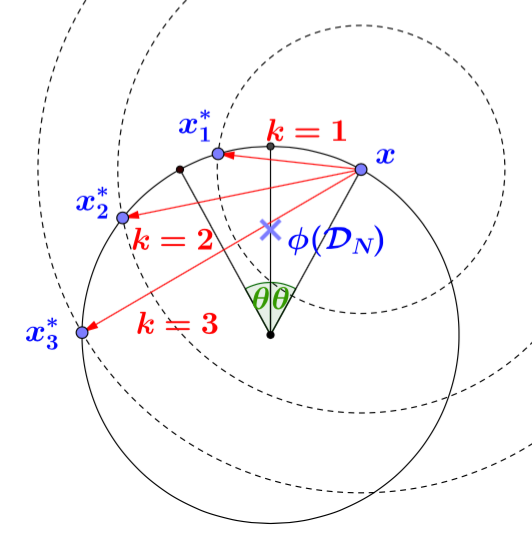
\includegraphics[width=0.6\textwidth]{ch-kemeny/figures/geomproof_big_r2k}
\end{center}
\caption{Geometric illustration of the bound in Lemma \ref{lemA:condition} with $x = \phi(\sigma)$ and $k=\frac{r^2}{4}$ taking integer values (representing possible Kendall's tau distance). The smallest integer value for $k$ such that these inequalities hold is $k=2$.}
\label{figA:illustration-condition}
\end{figure}


\subsection{Embedding of a Ball}

For $\sigma\in\Sn$ and $k\in\{0,\dots,\binom{n}{2}\}$ we denote by $B(\sigma,k)$ the (closed) ball for the Kendall's tau distance of center $\sigma$ and radius $k$, i.e. $B(\sigma,k) = \{\sigma'\in\Sn \;\vert\; d(\sigma,\sigma')\leq k\}$. The following is a direct consequence of Proposition \ref{propA:background-result}.

\begin{lemma}
\label{lemA:ball-embedding}
For $\sigma\in\Sn$ and $k\in\{0,\dots,\binom{n}{2}\}$,
\[
\phi\left( \Sn\setminus B(\sigma,k)\right) \; \subset \; \Sphere\setminus\mathcal{B}(\phi(\sigma),2\sqrt{k+1}) \,.
\]
\end{lemma}

\subsection{Proof of Theorem \ref{thmA:method}}

We can now prove Theorem \ref{thmA:method} by combining the previous results and observations.

\begin{proof}[Proof of Theorem \ref{thmA:method}]
Let $\DN\in\Sn^{N}$ be a dataset and $\sigma\in\Sn$ a permutation. By Lemma \ref{lemA:condition}, one has for any $r > 0$,
\begin{equation*}
\cos(\theta_{N}(\sigma)) > \sqrt{1 - \frac{r^{2}}{4R^{2}}} \Longrightarrow \min_{x\in\Sphere\setminus B(\phi(\sigma),r)}\theta_{N}(x) > \theta_{N}(\sigma) \,.
\end{equation*}
We take $r = 2\sqrt{k+1}$. The left-hand term becomes $\cos(\theta_{N}(\sigma)) > \sqrt{1 - \frac{k+1}{R^{2}}}$, which is the condition in Theorem \ref{thmA:method}. The right-hand term becomes:
\[
\min_{x\in\Sphere\setminus B(\phi(\sigma),2\sqrt{k+1})}\theta_{N}(x) > \theta_{N}(\sigma) \,,
\]
which implies by Lemma \ref{lemA:ball-embedding} that
\[
\min_{\sigma'\in\Sn\setminus B(\sigma,k)}\theta_{N}(\sigma') > \theta_{N}(\sigma) \,.
\]
This means that for all $\sigma'\in\Sn$ with $d(\sigma,\sigma') > k$, $\theta_{N}(\sigma') > \theta_{N}(\sigma)$. Now, by Lemma \ref{lemA:angles}, any Kemeny consensus $\sigstar$ necessarily satisfies $\theta_{N}(\sigstar) \leq \theta_{N}(\sigma)$. One therefore has $d(\sigma,\sigstar) \leq k$, and the proof is concluded.
\end{proof}



\section{Numerical Experiments}
\label{secA:experiments}


\subsection{Examples of Voting Rules}
\label{secA:votingrules}

In this section we study the tightness of the bound in Theorem \ref{thmA:method} and the applicability of The Method through numerical experiments. We first elaborate in detail the voting rules used in the chapter to approximate Kemeny's rule. Note that if multiple consensuses are returned from a rule on a given dataset, we always randomly pick one from these consensuses.

\begin{bulletList}
\item {\bf Positional scoring rules}. Given a scoring vector $w = (w_1,...,w_n) \in \RR^n$ of weights respectively for each alternative in $\n$, the $i$th alternative in a vote scores $w_i$. A total ranking is given by sorting the averaged scores over all votes, for example, the winner is the alternative with highest total score over all the votes. The \textbf{plurality} rule has the weight vector $(1,0,...,0)$, the \textbf{$k$-approval} rule has $(1,...,1,0...,0)$ containing 1s in the first $k$ positions, and the \textbf{Borda} rule \cite{Borda1781Memoire} has $(n, n-1, . . . , 1)$.
\item {\bf Copeland} \cite{Copeland1951reasonable}. A total ranking is given by sorting the Copeland scores averaged over all votes, for which the score of alternative $i$ is the number of pairwise beats, or $\#\{j \neq i: i \mbox{ beats } j\}$. For example, the Copeland winner is the alternative that wins the most pairwise elections.
\item {\bf QuickSort} \cite{Ali2012Experiments}. QuickSort recursively divides an unsorted list into two lists -- one list comprising alternatives that occur before a chosen index (called the \textit{pivot}), and another comprising alternatives that occur after, and then sorts each of the two lists. The pivot is always chosen as the first alternative.
\item {\bf Pick-a-Perm} \cite{Ali2012Experiments}. A total ranking is picked randomly from $\Sn$ according to the empirical distribution of the dataset $\DN$.
\item {\bf Plackett-Luce}. A Plackett-Luce ranking model defined for any $\sigma\in\Sn$ by $p_w(\sigma) = \prod_{i=1}^n w_{\sigma(i)}/\br{\sum_{j=i}^n w_{\sigma(j)}}$ parameterized by $w = (w_1,\dots,w_n)\in\RR^n$, fitted to $\DN$ by means of the MM algorithm \cite{Hunter2004MM}. A total ranking is then given by sorting $w$.
\item {\bf Pick-a-Random}. A total ranking is picked randomly from $\Sn$ according to uniform law (independent from $\DN$).
\end{bulletList}


Notably, Pick-a-Random is expected as a negative control experiment. To intuitively understand the rationale behind Pick-a-Random, let us consider the case conditioned on that the output of a voting rule has (at least) certain Kendall's tau distance to the Kemeny consensus. Compared to what Pick-a-Random would blindly pick any permutation without accessing to the dataset $\DN$ at all, a sensible voting rule should have a better chance to output one permutation with a smaller angle $\theta$ with $\phi(\DN)$ among all the permutations that share the same distance to Kemeny consensus. As we have reasoned in the geometric proof of The Method that the smaller the angle $\theta$ is, the more applicable our method will be, Pick-a-Random is expected to perform worse than other voting rules in terms of applicability of our method.



\subsection{Tightness of the Bound}

Recall that we denote by $n$ the number of alternatives, by $\DN\in\Sn^N$ any dataset, by $r$ any voting rule, and by $r(\DN)$ a consensus of $\DN$ given by $r$. For ease of notation convenience, we assume that $\KN$ contains a single consensus (otherwise we pick one randomly as we do in all experiments). The approximation efficiency of $r$ to Kemeny's rule is exactly measured by $d(r(\DN),\KN)$. Applying our method with $r(\DN)$ would return an upper bound for $d(r(\DN),\KN)$, that is: 
$$
d(r(\DN),\KN) \leq \kmin \,.
$$
Notably here we are not interested in studying the approximation efficiency of a particular voting rule, but we are rather interested in studying the approximation efficiency specific to our method indicated by the tightness of the bound, i.e.,
$$
s \br{r,\DN,n} := \kmin - d(r(\DN), \KN) \,.
$$
In other words, $s \br{r,\DN,n}$ quantifies how confident we are when we use $\kmin$ to ``approximate'' the approximation efficiency $d(r(\DN), \KN)$ of $r$ to Kemeny's rule on a given dataset $\DN$. The smaller $s \br{r,\DN,n}$ is, the better our method works when it is combined with the voting rule $r$ to pinpoint the Kemeny consensus on a given dataset $\DN$. Note that our notation stresses on the fact that $s$ depends typically on $\br{r,\DN,n}$. 


We empirically investigate the efficiency of our proposed method by experimenting $s \br{r,\DN,n}$ with various voting rules $r$, on different datasets $\DN$, implicitly involving $n$ as well. For that purpose, in each experiment we test six prevalent voting rules plus one negative-control method as approximate candidates to Kemeny's rule: three scoring rules that are Borda Count, $k$-approval, Copeland; two algorithmic approaches that are QuickSort and Pick-a-Perm; one statistical approach based on Plackett-Luce ranking model; one baseline method serving a negative control that is Pick-a-Random.


We first look at the the effect of different voting rules $r$ on $s \br{r;\DN,n}$ with the APA dataset. In the 1980 American Psychological Association (APA) presidential election, voters were asked to rank $n=5$ candidates in order of preference and a total of $N=5738$ complete ballots were reported. With the original collection of ballots introduced by \cite{Diaconis1989generalization}, We created $500$ bootstrapped pseudo-samples following \cite{Popova2012robust}. As shown in Figure \ref{figA:APA}, $s \br{r;\DN,n}$ varies across different voting rules and our method works typically well combined with Borda Count or Plackett-Luce, a phenomenon that constantly occurs in many experiments. For example for Borda Count the median tightness being $3$ means that our method provides a bound that tolerates an approximation within a Kendall's tau distance up to $3$. We also observe that on the contrary, the boxplot of Pick-a-Random always shows a wider range and larger median as expected. 


\begin{figure}[!htbp]
\begin{center}
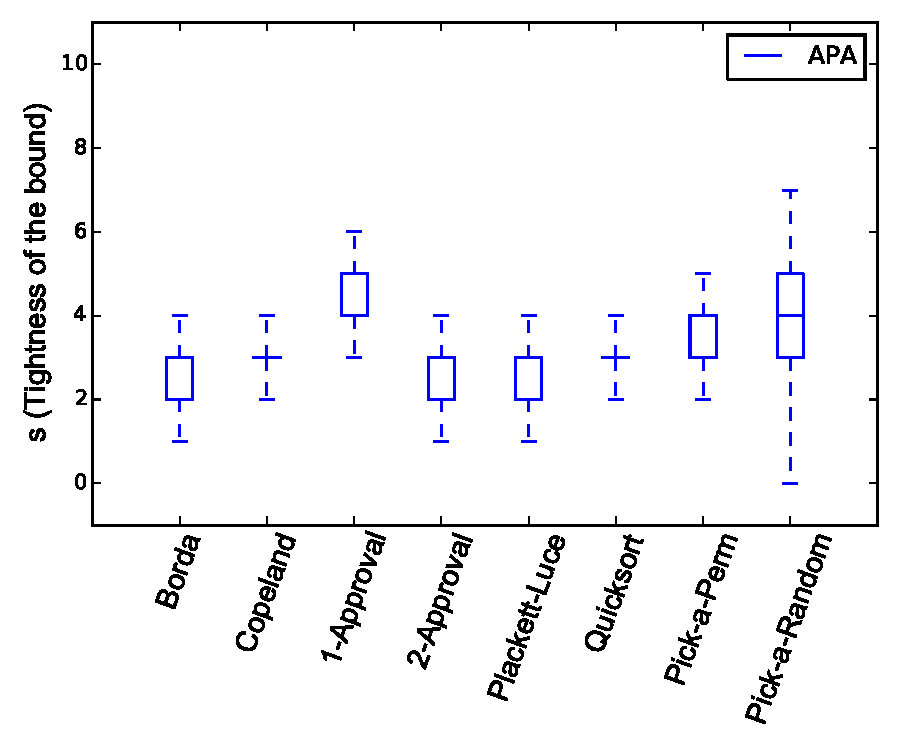
\includegraphics[width=0.6\textwidth]{ch-kemeny/experiments/APA.pdf}
\end{center}
\caption{Boxplots of $s \br{r,\DN,n}$ over sampling collections of datasets shows the effect from different voting rules $r$ with $500$ bootstrapped pseudo-samples of the APA dataset $(n=5,N=5738)$.}
\label{figA:APA}
\end{figure}


The effect of datasets $\DN$ on the measure $s \br{\DN;r,n}$ is tested with the Netflix data provided by \cite{Mattei2012empirical}. We set $n=3$ the number of ranked alternatives and take two types of data with distinct characteristics to contrast their impact: we took the $100$ datasets with a Condorcet winner and randomly selected $100$ datasets from those with no Condorcet winner. The rationale for this experiment is that Kemeny's rule is a Condorcet method, i.e., Kemeny's rule always yields a Condorcet winner if it exists. Therefore we suppose that the efficiency of our method should also depend on this particular social characteristic present in data. As expected, it is interesting to note the clear difference shown by the two types of data shown by Figure \ref{figA:netflix}. In words, our method is more efficient in case that a Condorcet winner is present in the dataset than the other case that a Condorcet winner is absent in the sense that $s$ is generally smaller in the former case.


\begin{figure}[!htbp]
\begin{center}
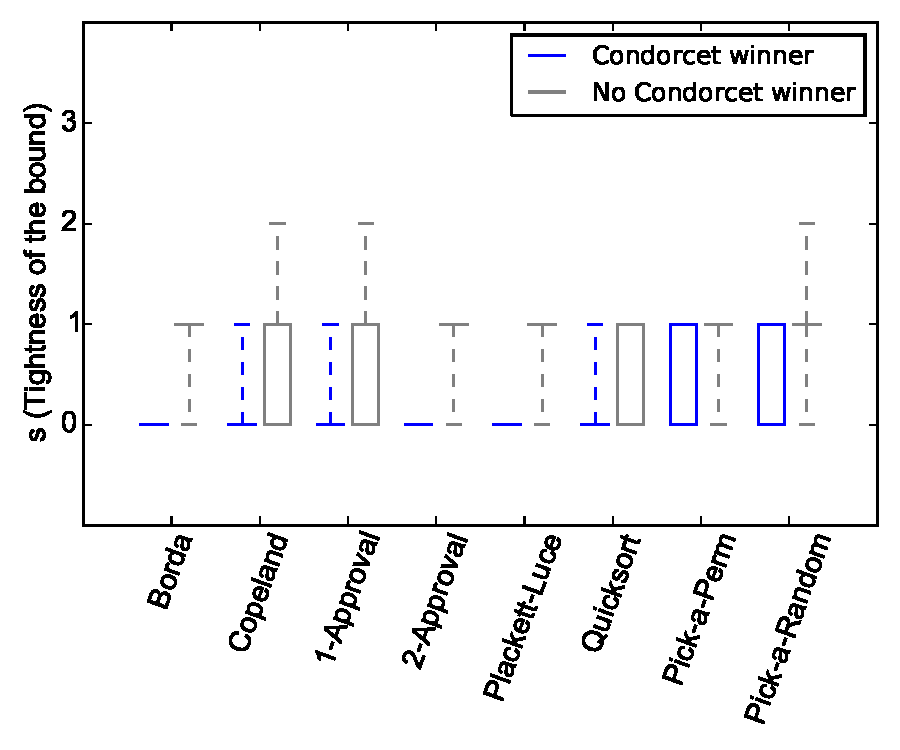
\includegraphics[width=0.6\textwidth]{ch-kemeny/experiments/netflix.pdf}
\end{center}
\caption{Boxplots of $s \br{r,\DN,n}$ over sampling collections of datasets shows the effect from datasets $\DN$. $100$ Netflix datasets with the presence of Condorcet winner and $100$ datasets with no Condorcet winner ($n=4$ and $N$ varies for each sample).}
\label{figA:netflix}
\end{figure}


We finally study how the $s \br{n;r,\DN}$ grows with the size of the alternative set $n$ using the sushi dataset found in \cite{Kamishima2003Nantonac}, originally provided as a dataset of $N=5000$ total rankings of $10$ sushi dishes. As evaluating $s$ requires exact Kemeny consensus which can quickly become intractable when $n$ is large, we strict in this study the number of sushi dishes $n$ to be relatively small, and generate collections of datasets, indexed by combinations of $n$ sushi dishes out of $\cbr{1,\dots,10}$, by counting the total occurrences of such order present in the original dataset. For example, when $n=3$ we have a total of ${10 \choose 3} = 120$ different combinations of alternatives (hence $120$ collections of datasets) each generated by counting the total occurrences of preference orders of individuals restricted to these $3$ alternatives. Therefore we have a total of $120;210;252$ datasets respectively for $n=3;4;5$. Figure \ref{figA:sushi} shows that $s \br{r,\DN,n}$ increases as $n$ grows, a trend that is dominant and consistent across all voting rules. Since the maximal distance ${n \choose 2}$ in $\Sn$ grows quadratically with respect to $n$, an interesting question would remain to specify explicitly the dependency of $\kmin$ on $n$, or the dependency of $s\br{r,\DN,n}$ on $n$, for a given voting rule.


\begin{figure}[!htbp]
\begin{center}
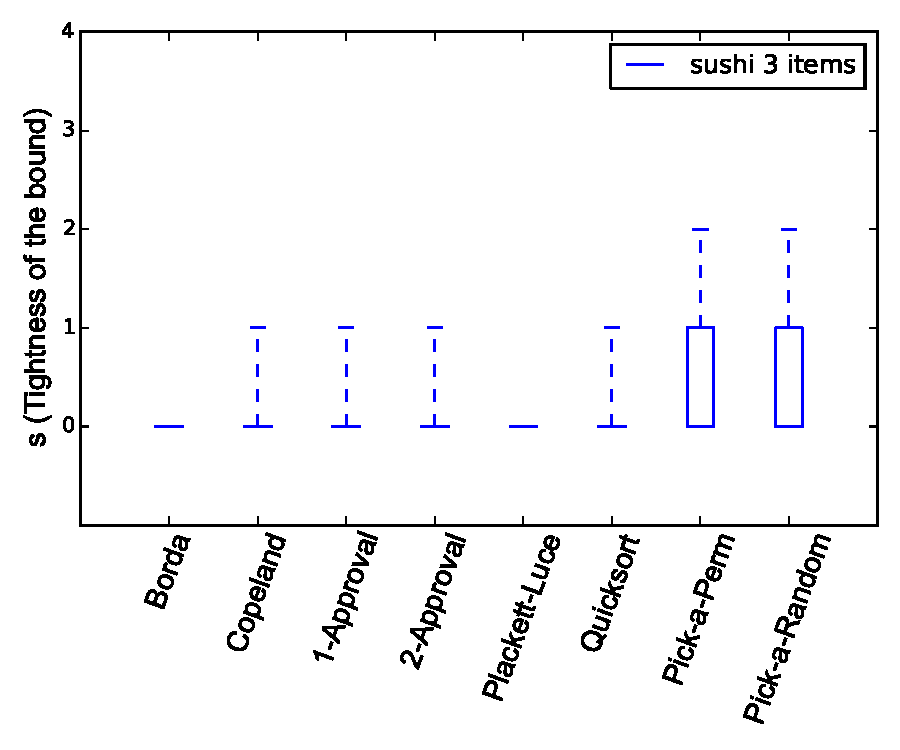
\includegraphics[width=0.3\textwidth]{ch-kemeny/experiments/sushi3.pdf}
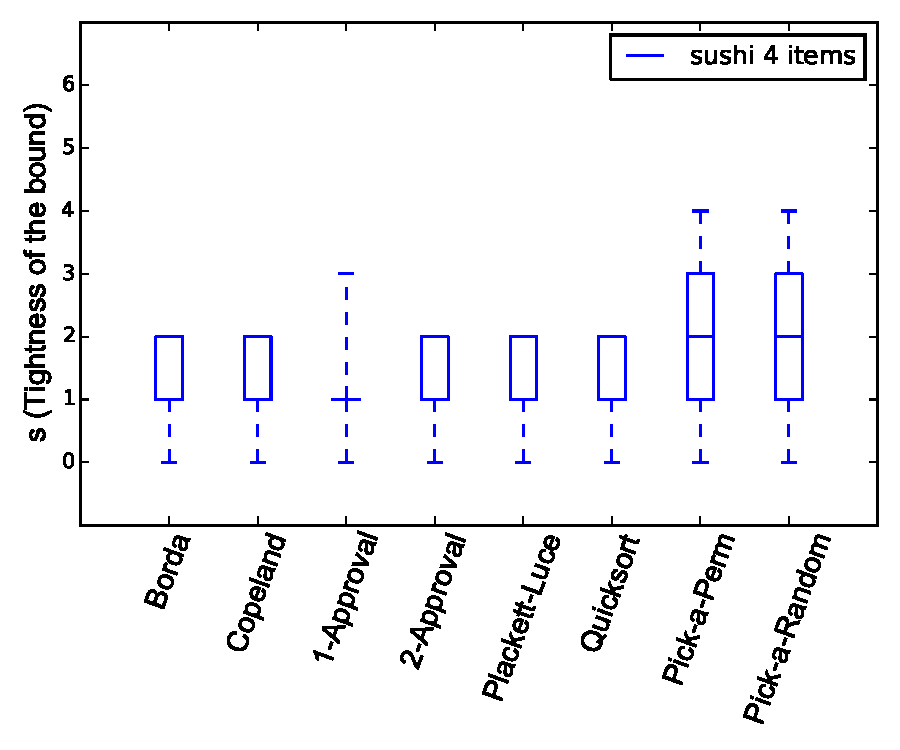
\includegraphics[width=0.3\textwidth]{ch-kemeny/experiments/sushi4.pdf}
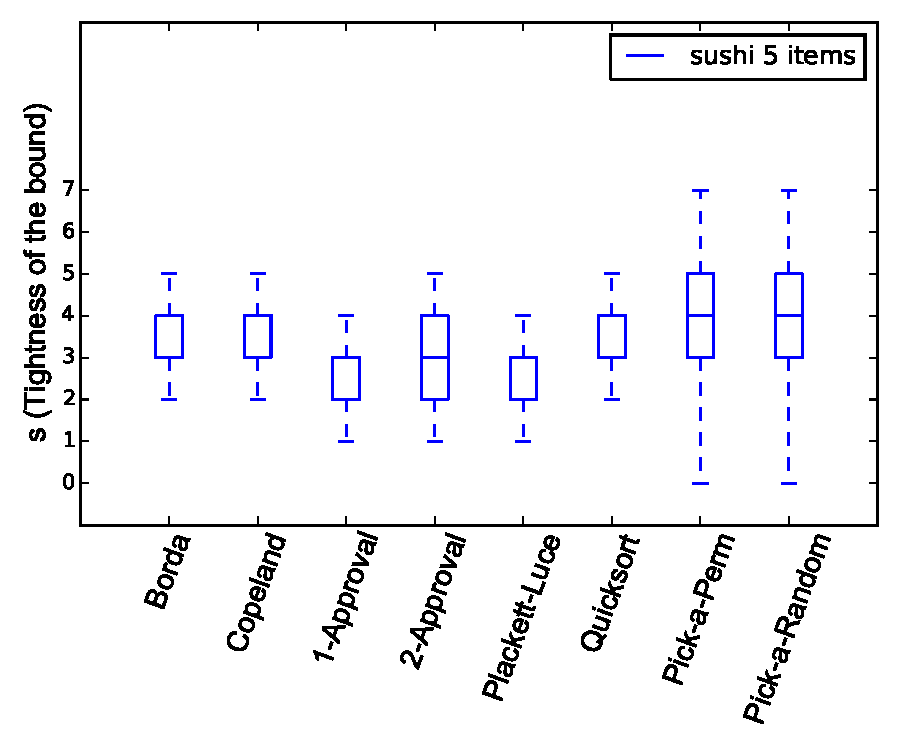
\includegraphics[width=0.3\textwidth]{ch-kemeny/experiments/sushi5.pdf}
\end{center}
\caption{Boxplots of $s \br{r,\DN,n}$ over sampling collections of datasets shows the effect from different size of alternative set $n$ with restricted sushi datasets $(n=3;4;5,N=5000)$.}
\label{figA:sushi}
\end{figure}




\subsection{Applicability of The Method} 

We have so far focused on small $n$ $(n \leq 5)$ case, and verified that our method is efficient in using $\kmin$ to approximate $d(r(\DN),\KN)$. We are now mostly interested in the usefulness of our method when $\kmin$ is directly combined with voting rules in pinpointing Kemeny consensus $\KN$ particularly when $n$ is large. Now we employ our method by using $\kmin$ for each dataset to upper bound the approximation performance of $r(\DN)$ to Kemeny's rule. Moreover, suppose that we are still interested in finding the exact Kemeny consensus despite a good approximation $r(\DN)$. Once we have computed an approximated ranking $r(\DN)$ and $\kmin$ is identified via our method, the search scope for the exact Kemeny consensuses can be narrowed down to those permutations within a distance of $\kmin$ to $r(\DN)$. Notably \cite[Lemma 1]{Wang2013rate} proved that the total number of such permutations in $\Sn$ is upper bounded by ${n + \kmin -1 \choose \kmin}$ which can be smaller than $\abs{\Sn} = n!$ by orders.



We took the original sushi dataset consisting of $N=5000$ individual votes on $n=10$ sushi dishes and created $500$ bootstrapped pseudo-samples following the same empirical distribution. Note that $\kmin$ should also depend on $\br{r,\DN,n}$. Since our bound is established in general with any $\sigma\in\Sn$ and does take into consideration the approximation efficiency of specific voting rules to Kemeny's rule, the predicted $\kmin$ should significantly rely on the approximate voting rules utilized and should be biased more in favor to voting rules with good approximation to Kemeny's rule since $\kmin$ can never be inferior to $d(r(\DN),\KN)$. As shown in Figure \ref{figA:applicability}, Pick-a-Random and Pick-a-Perm typically performs poorly, but this is largely due to the fact that the two voting rules are too naive to well approximate Kemeny's rule \textit{per se}. On the contrary, we observe that Borda, Copeland and QuickSort combined with our method best pinpoint Kemeny consensuses with $\kmin$ of a median distance $14$. This further means that in order to obtain all the exact Kemeny consensuses now, on average we need to search through at most ${10 + 14 -1 \choose 14} = 817,190$ permutations instead of $10! = 3,628,800$ permutations, where 77\% of permutations in $\mathbb{S}_{10}$ are removed from consideration.


\begin{figure}[!htbp]
\begin{center}
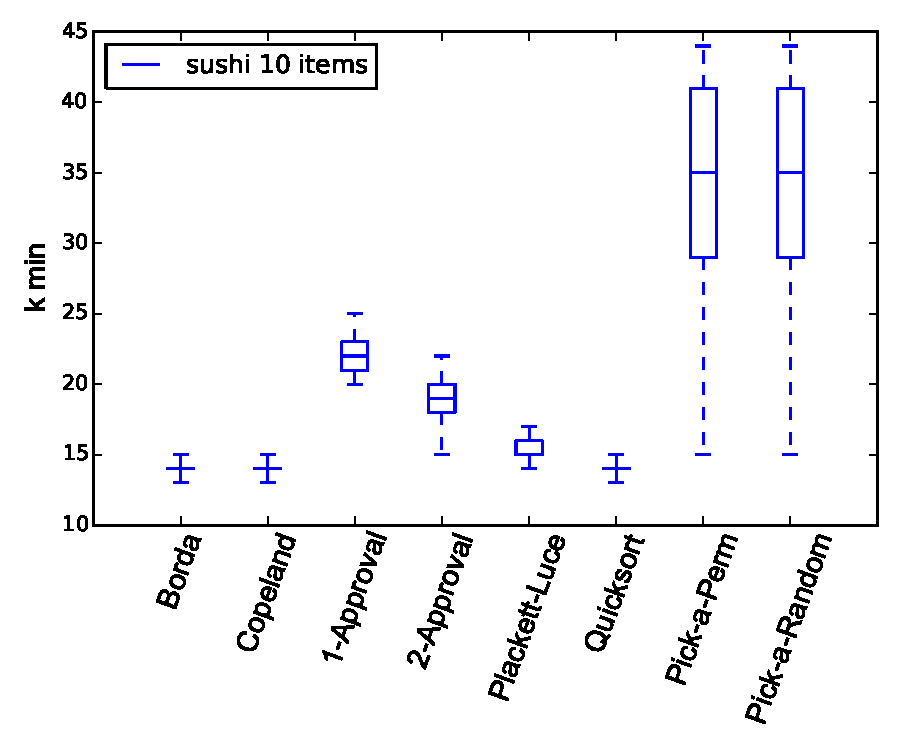
\includegraphics[width=0.6\textwidth]{ch-kemeny/experiments/sushi10.pdf}
\end{center}
\caption{Boxplots of $\kmin$ over $500$ bootstrapped pseudo-samples of the sushi dataset $(n=10, N=5000)$.}
\label{figA:applicability}
\end{figure}



\section{Discussion}

In this chapter, we have established a theoretical result that allows to control the Kendall's tau distance between a permutation and the Kemeny consensuses of any dataset. In practice, this provides a simple and general method to predict, for any ranking aggregation procedure, how close its output on a dataset is from the Kemeny consensuses. From a broader perspective, it constitutes a novel approach to apprehend the complexity of Kemeny aggregation.

Our results rely on the geometric properties of the Kendall embedding. Though it has rarely been used in the literature, it provides a powerful framework to analyze Kemeny aggregation. We therefore believe that it could pave way to other profound results. In particular, we deem that an analysis of how the embeddings of the permutation spread on the sphere could lead to a finer condition in Theorem \ref{thmA:method}, which is left as future work.

Another interesting direction would certainly be to extend our method to rank aggregation from partial orders, such as pairwise comparisons or top-$k$ rankings. Two main approaches can be followed. In the first one, a partial order would be identified with the set $S\subset\Sn$ of its linear extensions and its distance to a permutation $\sigma\in\Sn$ defined by the average $(1/\vert S\vert)\sum_{\sigma'\in S}d(\sigma,\sigma')$. The Kendall embedding would then naturally be extended to $S$ as $(1/\vert S\vert)\sum_{\sigma'\in S}\phi(\sigma')$, the barycenter of embeddings of its linear extensions. In the second approach, one would see a partial order as a collection of pairwise comparisons $\{i_{1}\succ j_{1}, \dots, i_{m}\succ j_{m}\}$ and define its distance to a permutation $\sigma\in\Sn$ by the average number of pairwise disagreements $(1/m)\sum_{r=1}^{m}\hollowone\{\sigma(i_{r}) > \sigma(j_{r})\}$. The Kendall embedding would then naturally be extended to $\{i_{1}\succ j_{1}, \dots, i_{m}\succ j_{m}\}$ as the embedding of any linear extension $\sigma$ where the coordinate on $\{i,j\}$ is put equal to $0$ if $\{i,j\}$ does not appear in the collection. In both cases, our approach would apply with slight changes to exploit related geometric properties.

\cleardoublepage

% bib
\bibliographystyle{mystyle}
\bibliography{mybib}

% index
% \printindex
% \cleardoublepage

\end{document}
